\subsection{Analisi dai dati digitali}
Si è usato il campione preso con il digitizer per fare un confronto tra le misure prese con l'apparato analogico e quelle prese digitalmente.\\
Per prima cosa è stato ricavato un segnale medio per canale, ottenendo così tempo di salita, di discesa e ampiezza media. I due grafici ottenuti sono mostrati in Fig. \ref{gr:mean_signal_0} e Fig. \ref{gr:mean_signal_1}

\begin{tikzpicture}
\pgfdeclareplotmark{cross} {
\pgfpathmoveto{\pgfpoint{-0.3\pgfplotmarksize}{\pgfplotmarksize}}
\pgfpathlineto{\pgfpoint{+0.3\pgfplotmarksize}{\pgfplotmarksize}}
\pgfpathlineto{\pgfpoint{+0.3\pgfplotmarksize}{0.3\pgfplotmarksize}}
\pgfpathlineto{\pgfpoint{+1\pgfplotmarksize}{0.3\pgfplotmarksize}}
\pgfpathlineto{\pgfpoint{+1\pgfplotmarksize}{-0.3\pgfplotmarksize}}
\pgfpathlineto{\pgfpoint{+0.3\pgfplotmarksize}{-0.3\pgfplotmarksize}}
\pgfpathlineto{\pgfpoint{+0.3\pgfplotmarksize}{-1.\pgfplotmarksize}}
\pgfpathlineto{\pgfpoint{-0.3\pgfplotmarksize}{-1.\pgfplotmarksize}}
\pgfpathlineto{\pgfpoint{-0.3\pgfplotmarksize}{-0.3\pgfplotmarksize}}
\pgfpathlineto{\pgfpoint{-1.\pgfplotmarksize}{-0.3\pgfplotmarksize}}
\pgfpathlineto{\pgfpoint{-1.\pgfplotmarksize}{0.3\pgfplotmarksize}}
\pgfpathlineto{\pgfpoint{-0.3\pgfplotmarksize}{0.3\pgfplotmarksize}}
\pgfpathclose
\pgfusepathqstroke
}
\pgfdeclareplotmark{cross*} {
\pgfpathmoveto{\pgfpoint{-0.3\pgfplotmarksize}{\pgfplotmarksize}}
\pgfpathlineto{\pgfpoint{+0.3\pgfplotmarksize}{\pgfplotmarksize}}
\pgfpathlineto{\pgfpoint{+0.3\pgfplotmarksize}{0.3\pgfplotmarksize}}
\pgfpathlineto{\pgfpoint{+1\pgfplotmarksize}{0.3\pgfplotmarksize}}
\pgfpathlineto{\pgfpoint{+1\pgfplotmarksize}{-0.3\pgfplotmarksize}}
\pgfpathlineto{\pgfpoint{+0.3\pgfplotmarksize}{-0.3\pgfplotmarksize}}
\pgfpathlineto{\pgfpoint{+0.3\pgfplotmarksize}{-1.\pgfplotmarksize}}
\pgfpathlineto{\pgfpoint{-0.3\pgfplotmarksize}{-1.\pgfplotmarksize}}
\pgfpathlineto{\pgfpoint{-0.3\pgfplotmarksize}{-0.3\pgfplotmarksize}}
\pgfpathlineto{\pgfpoint{-1.\pgfplotmarksize}{-0.3\pgfplotmarksize}}
\pgfpathlineto{\pgfpoint{-1.\pgfplotmarksize}{0.3\pgfplotmarksize}}
\pgfpathlineto{\pgfpoint{-0.3\pgfplotmarksize}{0.3\pgfplotmarksize}}
\pgfpathclose
\pgfusepathqfillstroke
}
\pgfdeclareplotmark{newstar} {
\pgfpathmoveto{\pgfqpoint{0pt}{\pgfplotmarksize}}
\pgfpathlineto{\pgfqpointpolar{44}{0.5\pgfplotmarksize}}
\pgfpathlineto{\pgfqpointpolar{18}{\pgfplotmarksize}}
\pgfpathlineto{\pgfqpointpolar{-20}{0.5\pgfplotmarksize}}
\pgfpathlineto{\pgfqpointpolar{-54}{\pgfplotmarksize}}
\pgfpathlineto{\pgfqpointpolar{-90}{0.5\pgfplotmarksize}}
\pgfpathlineto{\pgfqpointpolar{234}{\pgfplotmarksize}}
\pgfpathlineto{\pgfqpointpolar{198}{0.5\pgfplotmarksize}}
\pgfpathlineto{\pgfqpointpolar{162}{\pgfplotmarksize}}
\pgfpathlineto{\pgfqpointpolar{134}{0.5\pgfplotmarksize}}
\pgfpathclose
\pgfusepathqstroke
}
\pgfdeclareplotmark{newstar*} {
\pgfpathmoveto{\pgfqpoint{0pt}{\pgfplotmarksize}}
\pgfpathlineto{\pgfqpointpolar{44}{0.5\pgfplotmarksize}}
\pgfpathlineto{\pgfqpointpolar{18}{\pgfplotmarksize}}
\pgfpathlineto{\pgfqpointpolar{-20}{0.5\pgfplotmarksize}}
\pgfpathlineto{\pgfqpointpolar{-54}{\pgfplotmarksize}}
\pgfpathlineto{\pgfqpointpolar{-90}{0.5\pgfplotmarksize}}
\pgfpathlineto{\pgfqpointpolar{234}{\pgfplotmarksize}}
\pgfpathlineto{\pgfqpointpolar{198}{0.5\pgfplotmarksize}}
\pgfpathlineto{\pgfqpointpolar{162}{\pgfplotmarksize}}
\pgfpathlineto{\pgfqpointpolar{134}{0.5\pgfplotmarksize}}
\pgfpathclose
\pgfusepathqfillstroke
}
\definecolor{c}{rgb}{1,1,1};
\draw [color=c, fill=c] (0,0) rectangle (20,11.0085);
\draw [color=c, fill=c] (2,1.10085) rectangle (18,9.90762);
\definecolor{c}{rgb}{0,0,0};
\draw [c,line width=0.9] (2,1.10085) -- (2,9.90762) -- (18,9.90762) -- (18,1.10085) -- (2,1.10085);
\definecolor{c}{rgb}{1,1,1};
\draw [color=c, fill=c] (2,1.10085) rectangle (18,9.90762);
\definecolor{c}{rgb}{0,0,0};
\draw [c,line width=0.9] (2,1.10085) -- (2,9.90762) -- (18,9.90762) -- (18,1.10085) -- (2,1.10085);
\definecolor{c}{rgb}{0,0,0.6};
\draw [c,line width=0.9] (2,9.48742) -- (2.2,9.48742) -- (2.2,9.48742) -- (2.4,9.48742) -- (2.4,9.48742) -- (2.6,9.48742) -- (2.6,9.48742) -- (2.8,9.48742) -- (2.8,9.48742) -- (3,9.48742) -- (3,9.48743) -- (3.2,9.48743) -- (3.2,9.48741) --
 (3.4,9.48741) -- (3.4,9.48743) -- (3.6,9.48743) -- (3.6,9.48742) -- (3.8,9.48742) -- (3.8,9.48743) -- (4,9.48743) -- (4,9.48742) -- (4.2,9.48742) -- (4.2,9.48732) -- (4.4,9.48732) -- (4.4,9.48717) -- (4.6,9.48717) -- (4.6,9.48701) -- (4.8,9.48701)
 -- (4.8,9.4871) -- (5,9.4871) -- (5,9.4872) -- (5.2,9.4872) -- (5.2,9.48722) -- (5.4,9.48722) -- (5.4,9.48686) -- (5.6,9.48686) -- (5.6,9.4866) -- (5.8,9.4866) -- (5.8,9.48634) -- (6,9.48634) -- (6,9.4867) -- (6.2,9.4867) -- (6.2,9.48692) --
 (6.4,9.48692) -- (6.4,9.48716) -- (6.6,9.48716) -- (6.6,9.48721) -- (6.8,9.48721) -- (6.8,9.48726) -- (7,9.48726) -- (7,9.48728) -- (7.2,9.48728) -- (7.2,9.48728) -- (7.4,9.48728) -- (7.4,9.48739) -- (7.6,9.48739) -- (7.6,9.48825) -- (7.8,9.48825)
 -- (7.8,9.42433) -- (8,9.42433) -- (8,6.88473) -- (8.2,6.88473) -- (8.2,1.50025) -- (8.4,1.50025) -- (8.4,3.40203) -- (8.6,3.40203) -- (8.6,5.6249) -- (8.8,5.6249) -- (8.8,7.58763) -- (9,7.58763) -- (9,8.10377) -- (9.2,8.10377) -- (9.2,8.46759) --
 (9.4,8.46759) -- (9.4,8.54405) -- (9.6,8.54405) -- (9.6,8.79529) -- (9.8,8.79529) -- (9.8,9.09477) -- (10,9.09477) -- (10,9.29986) -- (10.2,9.29986) -- (10.2,9.44859) -- (10.4,9.44859) -- (10.4,9.30421) -- (10.6,9.30421) -- (10.6,9.26738) --
 (10.8,9.26738) -- (10.8,9.14727) -- (11,9.14727) -- (11,9.311) -- (11.2,9.311) -- (11.2,9.37002) -- (11.4,9.37002) -- (11.4,9.42704) -- (11.6,9.42704) -- (11.6,9.34394) -- (11.8,9.34394) -- (11.8,9.26105) -- (12,9.26105) -- (12,9.29597) --
 (12.2,9.29597) -- (12.2,9.33515) -- (12.4,9.33515) -- (12.4,9.43142) -- (12.6,9.43142) -- (12.6,9.37374) -- (12.8,9.37374) -- (12.8,9.35255) -- (13,9.35255) -- (13,9.29638) -- (13.2,9.29638) -- (13.2,9.34779) -- (13.4,9.34779) -- (13.4,9.39479) --
 (13.6,9.39479) -- (13.6,9.4125) -- (13.8,9.4125) -- (13.8,9.39562) -- (14,9.39562) -- (14,9.34477) -- (14.2,9.34477) -- (14.2,9.36443) -- (14.4,9.36443) -- (14.4,9.37936) -- (14.6,9.37936) -- (14.6,9.43012) -- (14.8,9.43012) -- (14.8,9.41434) --
 (15,9.41434) -- (15,9.40024) -- (15.2,9.40024) -- (15.2,9.37867) -- (15.4,9.37867) -- (15.4,9.39071) -- (15.6,9.39071) -- (15.6,9.42145) -- (15.8,9.42145) -- (15.8,9.42789) -- (16,9.42789) -- (16,9.42811) -- (16.2,9.42811) -- (16.2,9.40171) --
 (16.4,9.40171) -- (16.4,9.40894) -- (16.6,9.40894) -- (16.6,9.41635) -- (16.8,9.41635) -- (16.8,9.43939) -- (17,9.43939) -- (17,9.43886) -- (17.2,9.43886) -- (17.2,9.42956) -- (17.4,9.42956) -- (17.4,9.42241) -- (17.6,9.42241) -- (17.6,9.42278) --
 (17.8,9.42278) -- (17.8,9.43929) -- (18,9.43929);
\definecolor{c}{rgb}{0,0,0};
\draw [c,line width=0.9] (2,1.10085) -- (18,1.10085);
\draw [anchor= east] (18,0.484373) node[scale=0.854877, color=c, rotate=0]{t [ns]};
\draw [c,line width=0.9] (2,1.36505) -- (2,1.10085);
\draw [c,line width=0.9] (2.5,1.23295) -- (2.5,1.10085);
\draw [c,line width=0.9] (3,1.23295) -- (3,1.10085);
\draw [c,line width=0.9] (3.5,1.23295) -- (3.5,1.10085);
\draw [c,line width=0.9] (4,1.23295) -- (4,1.10085);
\draw [c,line width=0.9] (4.5,1.36505) -- (4.5,1.10085);
\draw [c,line width=0.9] (5,1.23295) -- (5,1.10085);
\draw [c,line width=0.9] (5.5,1.23295) -- (5.5,1.10085);
\draw [c,line width=0.9] (6,1.23295) -- (6,1.10085);
\draw [c,line width=0.9] (6.5,1.23295) -- (6.5,1.10085);
\draw [c,line width=0.9] (7,1.36505) -- (7,1.10085);
\draw [c,line width=0.9] (7.5,1.23295) -- (7.5,1.10085);
\draw [c,line width=0.9] (8,1.23295) -- (8,1.10085);
\draw [c,line width=0.9] (8.5,1.23295) -- (8.5,1.10085);
\draw [c,line width=0.9] (9,1.23295) -- (9,1.10085);
\draw [c,line width=0.9] (9.5,1.36505) -- (9.5,1.10085);
\draw [c,line width=0.9] (10,1.23295) -- (10,1.10085);
\draw [c,line width=0.9] (10.5,1.23295) -- (10.5,1.10085);
\draw [c,line width=0.9] (11,1.23295) -- (11,1.10085);
\draw [c,line width=0.9] (11.5,1.23295) -- (11.5,1.10085);
\draw [c,line width=0.9] (12,1.36505) -- (12,1.10085);
\draw [c,line width=0.9] (12.5,1.23295) -- (12.5,1.10085);
\draw [c,line width=0.9] (13,1.23295) -- (13,1.10085);
\draw [c,line width=0.9] (13.5,1.23295) -- (13.5,1.10085);
\draw [c,line width=0.9] (14,1.23295) -- (14,1.10085);
\draw [c,line width=0.9] (14.5,1.36505) -- (14.5,1.10085);
\draw [c,line width=0.9] (15,1.23295) -- (15,1.10085);
\draw [c,line width=0.9] (15.5,1.23295) -- (15.5,1.10085);
\draw [c,line width=0.9] (16,1.23295) -- (16,1.10085);
\draw [c,line width=0.9] (16.5,1.23295) -- (16.5,1.10085);
\draw [c,line width=0.9] (17,1.36505) -- (17,1.10085);
\draw [c,line width=0.9] (17,1.36505) -- (17,1.10085);
\draw [c,line width=0.9] (17.5,1.23295) -- (17.5,1.10085);
\draw [c,line width=0.9] (18,1.23295) -- (18,1.10085);
\draw [anchor=base] (2,0.737567) node[scale=0.854877, color=c, rotate=0]{0};
\draw [anchor=base] (4.5,0.737567) node[scale=0.854877, color=c, rotate=0]{50};
\draw [anchor=base] (7,0.737567) node[scale=0.854877, color=c, rotate=0]{100};
\draw [anchor=base] (9.5,0.737567) node[scale=0.854877, color=c, rotate=0]{150};
\draw [anchor=base] (12,0.737567) node[scale=0.854877, color=c, rotate=0]{200};
\draw [anchor=base] (14.5,0.737567) node[scale=0.854877, color=c, rotate=0]{250};
\draw [anchor=base] (17,0.737567) node[scale=0.854877, color=c, rotate=0]{300};
\draw [c,line width=0.9] (2,1.10085) -- (2,9.90762);
\draw [anchor= east] (0.88,9.90762) node[scale=0.854877, color=c, rotate=90]{Signal [a.u.]};
\draw [c,line width=0.9] (2.48,1.79993) -- (2,1.79993);
\draw [c,line width=0.9] (2.24,2.01837) -- (2,2.01837);
\draw [c,line width=0.9] (2.24,2.23681) -- (2,2.23681);
\draw [c,line width=0.9] (2.24,2.45525) -- (2,2.45525);
\draw [c,line width=0.9] (2.24,2.67369) -- (2,2.67369);
\draw [c,line width=0.9] (2.48,2.89213) -- (2,2.89213);
\draw [c,line width=0.9] (2.24,3.11056) -- (2,3.11056);
\draw [c,line width=0.9] (2.24,3.329) -- (2,3.329);
\draw [c,line width=0.9] (2.24,3.54744) -- (2,3.54744);
\draw [c,line width=0.9] (2.24,3.76588) -- (2,3.76588);
\draw [c,line width=0.9] (2.48,3.98432) -- (2,3.98432);
\draw [c,line width=0.9] (2.24,4.20276) -- (2,4.20276);
\draw [c,line width=0.9] (2.24,4.42119) -- (2,4.42119);
\draw [c,line width=0.9] (2.24,4.63963) -- (2,4.63963);
\draw [c,line width=0.9] (2.24,4.85807) -- (2,4.85807);
\draw [c,line width=0.9] (2.48,5.07651) -- (2,5.07651);
\draw [c,line width=0.9] (2.24,5.29495) -- (2,5.29495);
\draw [c,line width=0.9] (2.24,5.51339) -- (2,5.51339);
\draw [c,line width=0.9] (2.24,5.73182) -- (2,5.73182);
\draw [c,line width=0.9] (2.24,5.95026) -- (2,5.95026);
\draw [c,line width=0.9] (2.48,6.1687) -- (2,6.1687);
\draw [c,line width=0.9] (2.24,6.38714) -- (2,6.38714);
\draw [c,line width=0.9] (2.24,6.60558) -- (2,6.60558);
\draw [c,line width=0.9] (2.24,6.82402) -- (2,6.82402);
\draw [c,line width=0.9] (2.24,7.04245) -- (2,7.04245);
\draw [c,line width=0.9] (2.48,7.26089) -- (2,7.26089);
\draw [c,line width=0.9] (2.24,7.47933) -- (2,7.47933);
\draw [c,line width=0.9] (2.24,7.69777) -- (2,7.69777);
\draw [c,line width=0.9] (2.24,7.91621) -- (2,7.91621);
\draw [c,line width=0.9] (2.24,8.13464) -- (2,8.13464);
\draw [c,line width=0.9] (2.48,8.35308) -- (2,8.35308);
\draw [c,line width=0.9] (2.24,8.57152) -- (2,8.57152);
\draw [c,line width=0.9] (2.24,8.78996) -- (2,8.78996);
\draw [c,line width=0.9] (2.24,9.0084) -- (2,9.0084);
\draw [c,line width=0.9] (2.24,9.22684) -- (2,9.22684);
\draw [c,line width=0.9] (2.48,9.44528) -- (2,9.44528);
\draw [c,line width=0.9] (2.48,1.79993) -- (2,1.79993);
\draw [c,line width=0.9] (2.24,1.5815) -- (2,1.5815);
\draw [c,line width=0.9] (2.24,1.36306) -- (2,1.36306);
\draw [c,line width=0.9] (2.24,1.14462) -- (2,1.14462);
\draw [c,line width=0.9] (2.48,9.44528) -- (2,9.44528);
\draw [c,line width=0.9] (2.24,9.66371) -- (2,9.66371);
\draw [c,line width=0.9] (2.24,9.88215) -- (2,9.88215);
\draw [anchor= east] (1.9,1.79993) node[scale=0.854877, color=c, rotate=0]{2900};
\draw [anchor= east] (1.9,2.89213) node[scale=0.854877, color=c, rotate=0]{3000};
\draw [anchor= east] (1.9,3.98432) node[scale=0.854877, color=c, rotate=0]{3100};
\draw [anchor= east] (1.9,5.07651) node[scale=0.854877, color=c, rotate=0]{3200};
\draw [anchor= east] (1.9,6.1687) node[scale=0.854877, color=c, rotate=0]{3300};
\draw [anchor= east] (1.9,7.26089) node[scale=0.854877, color=c, rotate=0]{3400};
\draw [anchor= east] (1.9,8.35308) node[scale=0.854877, color=c, rotate=0]{3500};
\draw [anchor= east] (1.9,9.44528) node[scale=0.854877, color=c, rotate=0]{3600};
\end{tikzpicture}

\begin{tikzpicture}
\pgfdeclareplotmark{cross} {
\pgfpathmoveto{\pgfpoint{-0.3\pgfplotmarksize}{\pgfplotmarksize}}
\pgfpathlineto{\pgfpoint{+0.3\pgfplotmarksize}{\pgfplotmarksize}}
\pgfpathlineto{\pgfpoint{+0.3\pgfplotmarksize}{0.3\pgfplotmarksize}}
\pgfpathlineto{\pgfpoint{+1\pgfplotmarksize}{0.3\pgfplotmarksize}}
\pgfpathlineto{\pgfpoint{+1\pgfplotmarksize}{-0.3\pgfplotmarksize}}
\pgfpathlineto{\pgfpoint{+0.3\pgfplotmarksize}{-0.3\pgfplotmarksize}}
\pgfpathlineto{\pgfpoint{+0.3\pgfplotmarksize}{-1.\pgfplotmarksize}}
\pgfpathlineto{\pgfpoint{-0.3\pgfplotmarksize}{-1.\pgfplotmarksize}}
\pgfpathlineto{\pgfpoint{-0.3\pgfplotmarksize}{-0.3\pgfplotmarksize}}
\pgfpathlineto{\pgfpoint{-1.\pgfplotmarksize}{-0.3\pgfplotmarksize}}
\pgfpathlineto{\pgfpoint{-1.\pgfplotmarksize}{0.3\pgfplotmarksize}}
\pgfpathlineto{\pgfpoint{-0.3\pgfplotmarksize}{0.3\pgfplotmarksize}}
\pgfpathclose
\pgfusepathqstroke
}
\pgfdeclareplotmark{cross*} {
\pgfpathmoveto{\pgfpoint{-0.3\pgfplotmarksize}{\pgfplotmarksize}}
\pgfpathlineto{\pgfpoint{+0.3\pgfplotmarksize}{\pgfplotmarksize}}
\pgfpathlineto{\pgfpoint{+0.3\pgfplotmarksize}{0.3\pgfplotmarksize}}
\pgfpathlineto{\pgfpoint{+1\pgfplotmarksize}{0.3\pgfplotmarksize}}
\pgfpathlineto{\pgfpoint{+1\pgfplotmarksize}{-0.3\pgfplotmarksize}}
\pgfpathlineto{\pgfpoint{+0.3\pgfplotmarksize}{-0.3\pgfplotmarksize}}
\pgfpathlineto{\pgfpoint{+0.3\pgfplotmarksize}{-1.\pgfplotmarksize}}
\pgfpathlineto{\pgfpoint{-0.3\pgfplotmarksize}{-1.\pgfplotmarksize}}
\pgfpathlineto{\pgfpoint{-0.3\pgfplotmarksize}{-0.3\pgfplotmarksize}}
\pgfpathlineto{\pgfpoint{-1.\pgfplotmarksize}{-0.3\pgfplotmarksize}}
\pgfpathlineto{\pgfpoint{-1.\pgfplotmarksize}{0.3\pgfplotmarksize}}
\pgfpathlineto{\pgfpoint{-0.3\pgfplotmarksize}{0.3\pgfplotmarksize}}
\pgfpathclose
\pgfusepathqfillstroke
}
\pgfdeclareplotmark{newstar} {
\pgfpathmoveto{\pgfqpoint{0pt}{\pgfplotmarksize}}
\pgfpathlineto{\pgfqpointpolar{44}{0.5\pgfplotmarksize}}
\pgfpathlineto{\pgfqpointpolar{18}{\pgfplotmarksize}}
\pgfpathlineto{\pgfqpointpolar{-20}{0.5\pgfplotmarksize}}
\pgfpathlineto{\pgfqpointpolar{-54}{\pgfplotmarksize}}
\pgfpathlineto{\pgfqpointpolar{-90}{0.5\pgfplotmarksize}}
\pgfpathlineto{\pgfqpointpolar{234}{\pgfplotmarksize}}
\pgfpathlineto{\pgfqpointpolar{198}{0.5\pgfplotmarksize}}
\pgfpathlineto{\pgfqpointpolar{162}{\pgfplotmarksize}}
\pgfpathlineto{\pgfqpointpolar{134}{0.5\pgfplotmarksize}}
\pgfpathclose
\pgfusepathqstroke
}
\pgfdeclareplotmark{newstar*} {
\pgfpathmoveto{\pgfqpoint{0pt}{\pgfplotmarksize}}
\pgfpathlineto{\pgfqpointpolar{44}{0.5\pgfplotmarksize}}
\pgfpathlineto{\pgfqpointpolar{18}{\pgfplotmarksize}}
\pgfpathlineto{\pgfqpointpolar{-20}{0.5\pgfplotmarksize}}
\pgfpathlineto{\pgfqpointpolar{-54}{\pgfplotmarksize}}
\pgfpathlineto{\pgfqpointpolar{-90}{0.5\pgfplotmarksize}}
\pgfpathlineto{\pgfqpointpolar{234}{\pgfplotmarksize}}
\pgfpathlineto{\pgfqpointpolar{198}{0.5\pgfplotmarksize}}
\pgfpathlineto{\pgfqpointpolar{162}{\pgfplotmarksize}}
\pgfpathlineto{\pgfqpointpolar{134}{0.5\pgfplotmarksize}}
\pgfpathclose
\pgfusepathqfillstroke
}
\definecolor{c}{rgb}{1,1,1};
\draw [color=c, fill=c] (0,0) rectangle (20,11.0085);
\draw [color=c, fill=c] (2,1.10085) rectangle (18,9.90762);
\definecolor{c}{rgb}{0,0,0};
\draw [c,line width=0.9] (2,1.10085) -- (2,9.90762) -- (18,9.90762) -- (18,1.10085) -- (2,1.10085);
\definecolor{c}{rgb}{1,1,1};
\draw [color=c, fill=c] (2,1.10085) rectangle (18,9.90762);
\definecolor{c}{rgb}{0,0,0};
\draw [c,line width=0.9] (2,1.10085) -- (2,9.90762) -- (18,9.90762) -- (18,1.10085) -- (2,1.10085);
\definecolor{c}{rgb}{0,0,0.6};
\draw [c,line width=0.9] (2,9.48718) -- (2.2,9.48718) -- (2.2,9.48719) -- (2.4,9.48719) -- (2.4,9.48718) -- (2.6,9.48718) -- (2.6,9.48719) -- (2.8,9.48719) -- (2.8,9.4872) -- (3,9.4872) -- (3,9.48718) -- (3.2,9.48718) -- (3.2,9.48719) --
 (3.4,9.48719) -- (3.4,9.48719) -- (3.6,9.48719) -- (3.6,9.48719) -- (3.8,9.48719) -- (3.8,9.48719) -- (4,9.48719) -- (4,9.48719) -- (4.2,9.48719) -- (4.2,9.48717) -- (4.4,9.48717) -- (4.4,9.48696) -- (4.6,9.48696) -- (4.6,9.4868) -- (4.8,9.4868) --
 (4.8,9.48686) -- (5,9.48686) -- (5,9.48699) -- (5.2,9.48699) -- (5.2,9.48708) -- (5.4,9.48708) -- (5.4,9.48691) -- (5.6,9.48691) -- (5.6,9.48656) -- (5.8,9.48656) -- (5.8,9.48627) -- (6,9.48627) -- (6,9.48657) -- (6.2,9.48657) -- (6.2,9.4868) --
 (6.4,9.4868) -- (6.4,9.487) -- (6.6,9.487) -- (6.6,9.48703) -- (6.8,9.48703) -- (6.8,9.48703) -- (7,9.48703) -- (7,9.48704) -- (7.2,9.48704) -- (7.2,9.48705) -- (7.4,9.48705) -- (7.4,9.48715) -- (7.6,9.48715) -- (7.6,9.48825) -- (7.8,9.48825) --
 (7.8,9.41639) -- (8,9.41639) -- (8,6.64755) -- (8.2,6.64755) -- (8.2,1.50025) -- (8.4,1.50025) -- (8.4,3.6606) -- (8.6,3.6606) -- (8.6,5.81757) -- (8.8,5.81757) -- (8.8,7.7531) -- (9,7.7531) -- (9,8.51018) -- (9.2,8.51018) -- (9.2,8.91869) --
 (9.4,8.91869) -- (9.4,8.91475) -- (9.6,8.91475) -- (9.6,8.84305) -- (9.8,8.84305) -- (9.8,9.15593) -- (10,9.15593) -- (10,9.34825) -- (10.2,9.34825) -- (10.2,9.46495) -- (10.4,9.46495) -- (10.4,9.29036) -- (10.6,9.29036) -- (10.6,9.17963) --
 (10.8,9.17963) -- (10.8,9.19589) -- (11,9.19589) -- (11,9.31088) -- (11.2,9.31088) -- (11.2,9.43531) -- (11.4,9.43531) -- (11.4,9.34894) -- (11.6,9.34894) -- (11.6,9.28068) -- (11.8,9.28068) -- (11.8,9.22939) -- (12,9.22939) -- (12,9.3142) --
 (12.2,9.3142) -- (12.2,9.40517) -- (12.4,9.40517) -- (12.4,9.38847) -- (12.6,9.38847) -- (12.6,9.34441) -- (12.8,9.34441) -- (12.8,9.27973) -- (13,9.27973) -- (13,9.32617) -- (13.2,9.32617) -- (13.2,9.38578) -- (13.4,9.38578) -- (13.4,9.40897) --
 (13.6,9.40897) -- (13.6,9.38084) -- (13.8,9.38084) -- (13.8,9.32885) -- (14,9.32885) -- (14,9.34356) -- (14.2,9.34356) -- (14.2,9.37859) -- (14.4,9.37859) -- (14.4,9.41625) -- (14.6,9.41625) -- (14.6,9.40285) -- (14.8,9.40285) -- (14.8,9.37059) --
 (15,9.37059) -- (15,9.36481) -- (15.2,9.36481) -- (15.2,9.3841) -- (15.4,9.3841) -- (15.4,9.41908) -- (15.6,9.41908) -- (15.6,9.41745) -- (15.8,9.41745) -- (15.8,9.40115) -- (16,9.40115) -- (16,9.38652) -- (16.2,9.38652) -- (16.2,9.39608) --
 (16.4,9.39608) -- (16.4,9.42071) -- (16.6,9.42071) -- (16.6,9.42814) -- (16.8,9.42814) -- (16.8,9.42178) -- (17,9.42178) -- (17,9.40772) -- (17.2,9.40772) -- (17.2,9.41047) -- (17.4,9.41047) -- (17.4,9.42549) -- (17.6,9.42549) -- (17.6,9.43648) --
 (17.8,9.43648) -- (17.8,9.4356) -- (18,9.4356);
\definecolor{c}{rgb}{0,0,0};
\draw [c,line width=0.9] (2,1.10085) -- (18,1.10085);
\draw [anchor= east] (18,0.484373) node[scale=0.854877, color=c, rotate=0]{t [ns]};
\draw [c,line width=0.9] (2,1.36505) -- (2,1.10085);
\draw [c,line width=0.9] (2.5,1.23295) -- (2.5,1.10085);
\draw [c,line width=0.9] (3,1.23295) -- (3,1.10085);
\draw [c,line width=0.9] (3.5,1.23295) -- (3.5,1.10085);
\draw [c,line width=0.9] (4,1.23295) -- (4,1.10085);
\draw [c,line width=0.9] (4.5,1.36505) -- (4.5,1.10085);
\draw [c,line width=0.9] (5,1.23295) -- (5,1.10085);
\draw [c,line width=0.9] (5.5,1.23295) -- (5.5,1.10085);
\draw [c,line width=0.9] (6,1.23295) -- (6,1.10085);
\draw [c,line width=0.9] (6.5,1.23295) -- (6.5,1.10085);
\draw [c,line width=0.9] (7,1.36505) -- (7,1.10085);
\draw [c,line width=0.9] (7.5,1.23295) -- (7.5,1.10085);
\draw [c,line width=0.9] (8,1.23295) -- (8,1.10085);
\draw [c,line width=0.9] (8.5,1.23295) -- (8.5,1.10085);
\draw [c,line width=0.9] (9,1.23295) -- (9,1.10085);
\draw [c,line width=0.9] (9.5,1.36505) -- (9.5,1.10085);
\draw [c,line width=0.9] (10,1.23295) -- (10,1.10085);
\draw [c,line width=0.9] (10.5,1.23295) -- (10.5,1.10085);
\draw [c,line width=0.9] (11,1.23295) -- (11,1.10085);
\draw [c,line width=0.9] (11.5,1.23295) -- (11.5,1.10085);
\draw [c,line width=0.9] (12,1.36505) -- (12,1.10085);
\draw [c,line width=0.9] (12.5,1.23295) -- (12.5,1.10085);
\draw [c,line width=0.9] (13,1.23295) -- (13,1.10085);
\draw [c,line width=0.9] (13.5,1.23295) -- (13.5,1.10085);
\draw [c,line width=0.9] (14,1.23295) -- (14,1.10085);
\draw [c,line width=0.9] (14.5,1.36505) -- (14.5,1.10085);
\draw [c,line width=0.9] (15,1.23295) -- (15,1.10085);
\draw [c,line width=0.9] (15.5,1.23295) -- (15.5,1.10085);
\draw [c,line width=0.9] (16,1.23295) -- (16,1.10085);
\draw [c,line width=0.9] (16.5,1.23295) -- (16.5,1.10085);
\draw [c,line width=0.9] (17,1.36505) -- (17,1.10085);
\draw [c,line width=0.9] (17,1.36505) -- (17,1.10085);
\draw [c,line width=0.9] (17.5,1.23295) -- (17.5,1.10085);
\draw [c,line width=0.9] (18,1.23295) -- (18,1.10085);
\draw [anchor=base] (2,0.737567) node[scale=0.854877, color=c, rotate=0]{0};
\draw [anchor=base] (4.5,0.737567) node[scale=0.854877, color=c, rotate=0]{50};
\draw [anchor=base] (7,0.737567) node[scale=0.854877, color=c, rotate=0]{100};
\draw [anchor=base] (9.5,0.737567) node[scale=0.854877, color=c, rotate=0]{150};
\draw [anchor=base] (12,0.737567) node[scale=0.854877, color=c, rotate=0]{200};
\draw [anchor=base] (14.5,0.737567) node[scale=0.854877, color=c, rotate=0]{250};
\draw [anchor=base] (17,0.737567) node[scale=0.854877, color=c, rotate=0]{300};
\draw [c,line width=0.9] (2,1.10085) -- (2,9.90762);
\draw [anchor= east] (0.88,9.90762) node[scale=0.854877, color=c, rotate=90]{Signal [a.u.]};
\draw [c,line width=0.9] (2.48,1.1948) -- (2,1.1948);
\draw [c,line width=0.9] (2.24,1.44684) -- (2,1.44684);
\draw [c,line width=0.9] (2.24,1.69889) -- (2,1.69889);
\draw [c,line width=0.9] (2.24,1.95093) -- (2,1.95093);
\draw [c,line width=0.9] (2.24,2.20298) -- (2,2.20298);
\draw [c,line width=0.9] (2.48,2.45502) -- (2,2.45502);
\draw [c,line width=0.9] (2.24,2.70707) -- (2,2.70707);
\draw [c,line width=0.9] (2.24,2.95912) -- (2,2.95912);
\draw [c,line width=0.9] (2.24,3.21116) -- (2,3.21116);
\draw [c,line width=0.9] (2.24,3.46321) -- (2,3.46321);
\draw [c,line width=0.9] (2.48,3.71525) -- (2,3.71525);
\draw [c,line width=0.9] (2.24,3.9673) -- (2,3.9673);
\draw [c,line width=0.9] (2.24,4.21934) -- (2,4.21934);
\draw [c,line width=0.9] (2.24,4.47139) -- (2,4.47139);
\draw [c,line width=0.9] (2.24,4.72344) -- (2,4.72344);
\draw [c,line width=0.9] (2.48,4.97548) -- (2,4.97548);
\draw [c,line width=0.9] (2.24,5.22753) -- (2,5.22753);
\draw [c,line width=0.9] (2.24,5.47957) -- (2,5.47957);
\draw [c,line width=0.9] (2.24,5.73162) -- (2,5.73162);
\draw [c,line width=0.9] (2.24,5.98366) -- (2,5.98366);
\draw [c,line width=0.9] (2.48,6.23571) -- (2,6.23571);
\draw [c,line width=0.9] (2.24,6.48775) -- (2,6.48775);
\draw [c,line width=0.9] (2.24,6.7398) -- (2,6.7398);
\draw [c,line width=0.9] (2.24,6.99185) -- (2,6.99185);
\draw [c,line width=0.9] (2.24,7.24389) -- (2,7.24389);
\draw [c,line width=0.9] (2.48,7.49594) -- (2,7.49594);
\draw [c,line width=0.9] (2.24,7.74798) -- (2,7.74798);
\draw [c,line width=0.9] (2.24,8.00003) -- (2,8.00003);
\draw [c,line width=0.9] (2.24,8.25207) -- (2,8.25207);
\draw [c,line width=0.9] (2.24,8.50412) -- (2,8.50412);
\draw [c,line width=0.9] (2.48,8.75617) -- (2,8.75617);
\draw [c,line width=0.9] (2.48,1.1948) -- (2,1.1948);
\draw [c,line width=0.9] (2.48,8.75617) -- (2,8.75617);
\draw [c,line width=0.9] (2.24,9.00821) -- (2,9.00821);
\draw [c,line width=0.9] (2.24,9.26026) -- (2,9.26026);
\draw [c,line width=0.9] (2.24,9.5123) -- (2,9.5123);
\draw [c,line width=0.9] (2.24,9.76435) -- (2,9.76435);
\draw [anchor= east] (1.9,1.1948) node[scale=0.854877, color=c, rotate=0]{3100};
\draw [anchor= east] (1.9,2.45502) node[scale=0.854877, color=c, rotate=0]{3200};
\draw [anchor= east] (1.9,3.71525) node[scale=0.854877, color=c, rotate=0]{3300};
\draw [anchor= east] (1.9,4.97548) node[scale=0.854877, color=c, rotate=0]{3400};
\draw [anchor= east] (1.9,6.23571) node[scale=0.854877, color=c, rotate=0]{3500};
\draw [anchor= east] (1.9,7.49594) node[scale=0.854877, color=c, rotate=0]{3600};
\draw [anchor= east] (1.9,8.75617) node[scale=0.854877, color=c, rotate=0]{3700};
\definecolor{c}{rgb}{1,1,1};
\draw [color=c, fill=c] (15.6,8.53156) rectangle (19.6,10.2929);
\definecolor{c}{rgb}{0,0,0};
\draw [c,line width=0.9] (15.6,8.53156) -- (19.6,8.53156);
\draw [c,line width=0.9] (19.6,8.53156) -- (19.6,10.2929);
\draw [c,line width=0.9] (19.6,10.2929) -- (15.6,10.2929);
\draw [c,line width=0.9] (15.6,10.2929) -- (15.6,8.53156);
\draw (17.6,10.0727) node[scale=0.889072, color=c, rotate=0]{MeanSignalCh1};
\draw [c,line width=0.9] (15.6,9.85258) -- (19.6,9.85258);
\draw [anchor= west] (15.8,9.63241) node[scale=0.889072, color=c, rotate=0]{Entries };
\draw [anchor= east] (19.4,9.63241) node[scale=0.889072, color=c, rotate=0]{ 0};
\draw [anchor= west] (15.8,9.19207) node[scale=0.889072, color=c, rotate=0]{Mean  };
\draw [anchor= east] (19.4,9.19207) node[scale=0.889072, color=c, rotate=0]{      0};
\draw [anchor= west] (15.8,8.75173) node[scale=0.889072, color=c, rotate=0]{Std Dev   };
\draw [anchor= east] (19.4,8.75173) node[scale=0.889072, color=c, rotate=0]{      0};
\end{tikzpicture}


Tabella bella

Filtrando dal campione solo gli eventi in coincidenza (presa contando gli eventi il cui time tag differisse meno di 100 ns), si è poi fatta un analisi della risoluzione temporale dell'apparato digitale. Per le misure di tempo si è usato un algoritmo simile al CFTD analogico, facendo variare il ritardo tra i 4 e i 12 ns e l'attenuazione tra lo 0.2 e lo 0.8. Per la ricerca del punto di zero cressing si è fatta un interpolazione con una cubica tra i punti di massimo e minimo del segnale di ``CF monitor'', dato che l'interpolazione suggerita con una retta aveva diversi problemi dovuti alla bassa frequenza di campionamento (vedi Fig. \ref{gr:fail_retta_interp}) che davano una distribuzione temporale distorta.
Le distribuzioni ottenute al variare dei parametri sono state sovrapposte in Fig. \ref{hist:confronto_ris_temp_digi}, mostrando che la risoluzione migliore si ha quando il ritardo è di 4 ns e l'attenuazione è a 0.3. Dato però che questa distribuzione risulta essere leggermente deformata, si è preferito usare l'attenuazione a 0.4, la seconda migliore.

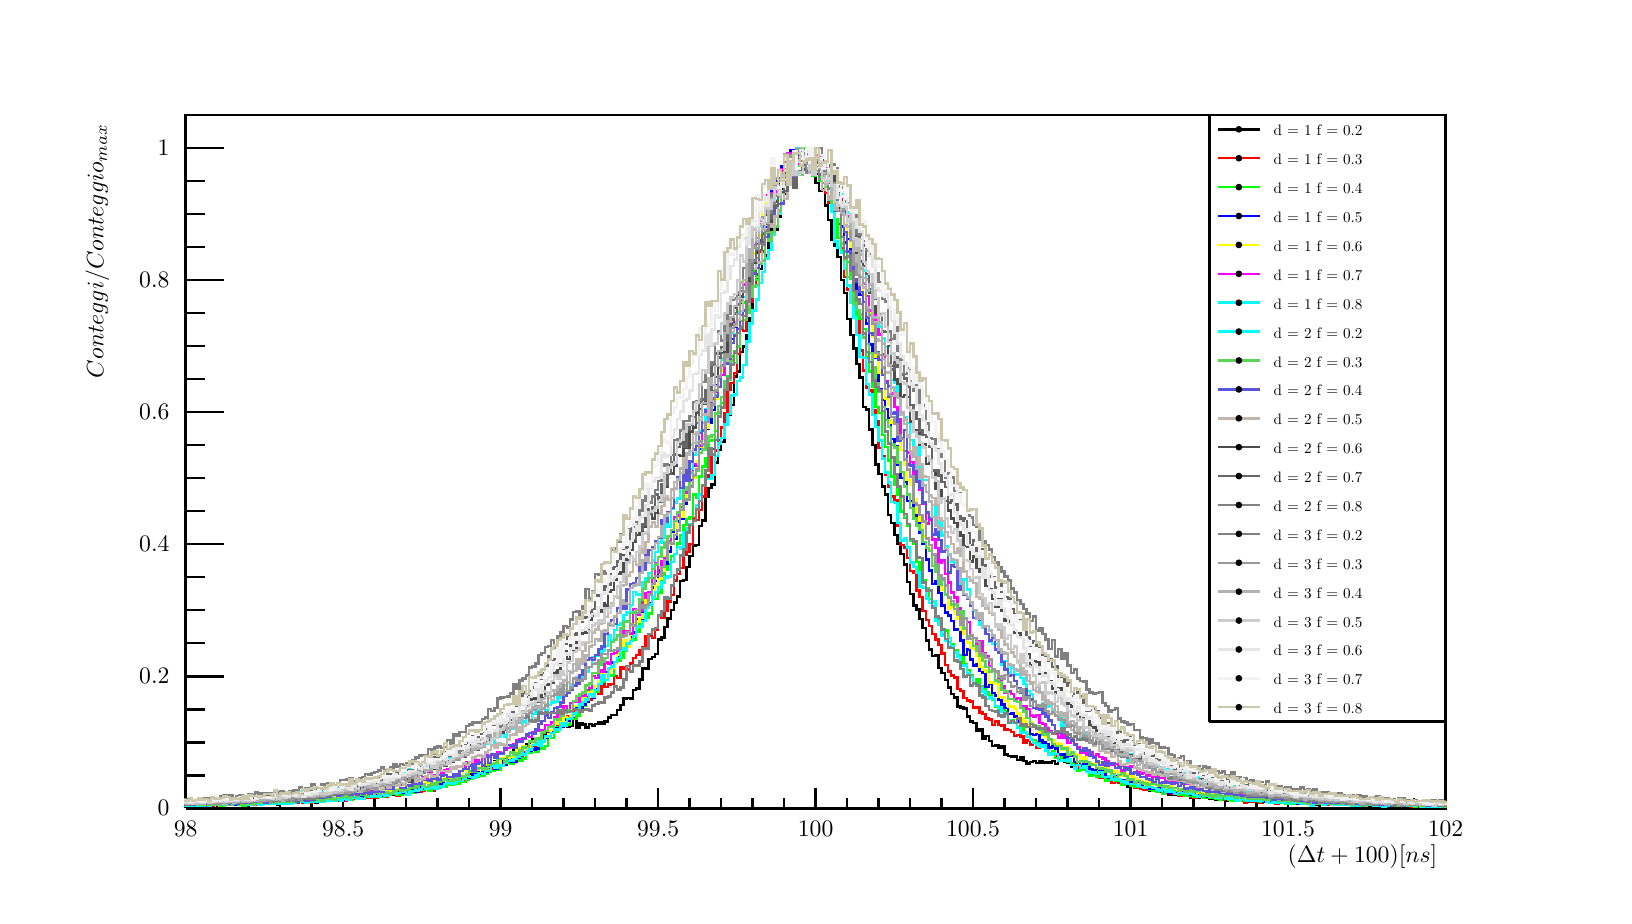
\begin{tikzpicture}
\pgfdeclareplotmark{cross} {
\pgfpathmoveto{\pgfpoint{-0.3\pgfplotmarksize}{\pgfplotmarksize}}
\pgfpathlineto{\pgfpoint{+0.3\pgfplotmarksize}{\pgfplotmarksize}}
\pgfpathlineto{\pgfpoint{+0.3\pgfplotmarksize}{0.3\pgfplotmarksize}}
\pgfpathlineto{\pgfpoint{+1\pgfplotmarksize}{0.3\pgfplotmarksize}}
\pgfpathlineto{\pgfpoint{+1\pgfplotmarksize}{-0.3\pgfplotmarksize}}
\pgfpathlineto{\pgfpoint{+0.3\pgfplotmarksize}{-0.3\pgfplotmarksize}}
\pgfpathlineto{\pgfpoint{+0.3\pgfplotmarksize}{-1.\pgfplotmarksize}}
\pgfpathlineto{\pgfpoint{-0.3\pgfplotmarksize}{-1.\pgfplotmarksize}}
\pgfpathlineto{\pgfpoint{-0.3\pgfplotmarksize}{-0.3\pgfplotmarksize}}
\pgfpathlineto{\pgfpoint{-1.\pgfplotmarksize}{-0.3\pgfplotmarksize}}
\pgfpathlineto{\pgfpoint{-1.\pgfplotmarksize}{0.3\pgfplotmarksize}}
\pgfpathlineto{\pgfpoint{-0.3\pgfplotmarksize}{0.3\pgfplotmarksize}}
\pgfpathclose
\pgfusepathqstroke
}
\pgfdeclareplotmark{cross*} {
\pgfpathmoveto{\pgfpoint{-0.3\pgfplotmarksize}{\pgfplotmarksize}}
\pgfpathlineto{\pgfpoint{+0.3\pgfplotmarksize}{\pgfplotmarksize}}
\pgfpathlineto{\pgfpoint{+0.3\pgfplotmarksize}{0.3\pgfplotmarksize}}
\pgfpathlineto{\pgfpoint{+1\pgfplotmarksize}{0.3\pgfplotmarksize}}
\pgfpathlineto{\pgfpoint{+1\pgfplotmarksize}{-0.3\pgfplotmarksize}}
\pgfpathlineto{\pgfpoint{+0.3\pgfplotmarksize}{-0.3\pgfplotmarksize}}
\pgfpathlineto{\pgfpoint{+0.3\pgfplotmarksize}{-1.\pgfplotmarksize}}
\pgfpathlineto{\pgfpoint{-0.3\pgfplotmarksize}{-1.\pgfplotmarksize}}
\pgfpathlineto{\pgfpoint{-0.3\pgfplotmarksize}{-0.3\pgfplotmarksize}}
\pgfpathlineto{\pgfpoint{-1.\pgfplotmarksize}{-0.3\pgfplotmarksize}}
\pgfpathlineto{\pgfpoint{-1.\pgfplotmarksize}{0.3\pgfplotmarksize}}
\pgfpathlineto{\pgfpoint{-0.3\pgfplotmarksize}{0.3\pgfplotmarksize}}
\pgfpathclose
\pgfusepathqfillstroke
}
\pgfdeclareplotmark{newstar} {
\pgfpathmoveto{\pgfqpoint{0pt}{\pgfplotmarksize}}
\pgfpathlineto{\pgfqpointpolar{44}{0.5\pgfplotmarksize}}
\pgfpathlineto{\pgfqpointpolar{18}{\pgfplotmarksize}}
\pgfpathlineto{\pgfqpointpolar{-20}{0.5\pgfplotmarksize}}
\pgfpathlineto{\pgfqpointpolar{-54}{\pgfplotmarksize}}
\pgfpathlineto{\pgfqpointpolar{-90}{0.5\pgfplotmarksize}}
\pgfpathlineto{\pgfqpointpolar{234}{\pgfplotmarksize}}
\pgfpathlineto{\pgfqpointpolar{198}{0.5\pgfplotmarksize}}
\pgfpathlineto{\pgfqpointpolar{162}{\pgfplotmarksize}}
\pgfpathlineto{\pgfqpointpolar{134}{0.5\pgfplotmarksize}}
\pgfpathclose
\pgfusepathqstroke
}
\pgfdeclareplotmark{newstar*} {
\pgfpathmoveto{\pgfqpoint{0pt}{\pgfplotmarksize}}
\pgfpathlineto{\pgfqpointpolar{44}{0.5\pgfplotmarksize}}
\pgfpathlineto{\pgfqpointpolar{18}{\pgfplotmarksize}}
\pgfpathlineto{\pgfqpointpolar{-20}{0.5\pgfplotmarksize}}
\pgfpathlineto{\pgfqpointpolar{-54}{\pgfplotmarksize}}
\pgfpathlineto{\pgfqpointpolar{-90}{0.5\pgfplotmarksize}}
\pgfpathlineto{\pgfqpointpolar{234}{\pgfplotmarksize}}
\pgfpathlineto{\pgfqpointpolar{198}{0.5\pgfplotmarksize}}
\pgfpathlineto{\pgfqpointpolar{162}{\pgfplotmarksize}}
\pgfpathlineto{\pgfqpointpolar{134}{0.5\pgfplotmarksize}}
\pgfpathclose
\pgfusepathqfillstroke
}
\definecolor{c}{rgb}{1,1,1};
\draw [color=c, fill=c] (0,0) rectangle (20,11.0085);
\draw [color=c, fill=c] (2,1.10085) rectangle (18,9.90762);
\definecolor{c}{rgb}{0,0,0};
\draw [c,line width=0.9] (2,1.10085) -- (2,9.90762) -- (18,9.90762) -- (18,1.10085) -- (2,1.10085);
\definecolor{c}{rgb}{1,1,1};
\draw [color=c, fill=c] (2,1.10085) rectangle (18,9.90762);
\definecolor{c}{rgb}{0,0,0};
\draw [c,line width=0.9] (2,1.10085) -- (2,9.90762) -- (18,9.90762) -- (18,1.10085) -- (2,1.10085);
\draw [c,line width=0.9] (2,1.15005) -- (2.04,1.15005) -- (2.04,1.13702) -- (2.08,1.13702) -- (2.08,1.14137) -- (2.12,1.14137) -- (2.12,1.14643) -- (2.16,1.14643) -- (2.16,1.14571) -- (2.2,1.14571) -- (2.2,1.15367) -- (2.24,1.15367) -- (2.24,1.14064)
 -- (2.28,1.14064) -- (2.28,1.1515) -- (2.32,1.1515) -- (2.32,1.14281) -- (2.36,1.14281) -- (2.36,1.15005) -- (2.4,1.15005) -- (2.4,1.14715) -- (2.44,1.14715) -- (2.44,1.15294) -- (2.48,1.15294) -- (2.48,1.14932) -- (2.52,1.14932) -- (2.52,1.14788)
 -- (2.56,1.14788) -- (2.56,1.14571) -- (2.6,1.14571) -- (2.6,1.15222) -- (2.64,1.15222) -- (2.64,1.15222) -- (2.68,1.15222) -- (2.68,1.16235) -- (2.72,1.16235) -- (2.72,1.15656) -- (2.76,1.15656) -- (2.76,1.15945) -- (2.8,1.15945) -- (2.8,1.16524)
 -- (2.84,1.16524) -- (2.84,1.16452) -- (2.88,1.16452) -- (2.88,1.16597) -- (2.92,1.16597) -- (2.92,1.17031) -- (2.96,1.17031) -- (2.96,1.16669) -- (3,1.16669) -- (3,1.15801) -- (3.04,1.15801) -- (3.04,1.16452) -- (3.08,1.16452) -- (3.08,1.18188) --
 (3.12,1.18188) -- (3.12,1.17971) -- (3.16,1.17971) -- (3.16,1.15294) -- (3.2,1.15294) -- (3.2,1.17175) -- (3.24,1.17175) -- (3.24,1.18261) -- (3.28,1.18261) -- (3.28,1.16958) -- (3.32,1.16958) -- (3.32,1.1761) -- (3.36,1.1761) -- (3.36,1.17248) --
 (3.4,1.17248) -- (3.4,1.17682) -- (3.44,1.17682) -- (3.44,1.19201) -- (3.48,1.19201) -- (3.48,1.1732) -- (3.52,1.1732) -- (3.52,1.18984) -- (3.56,1.18984) -- (3.56,1.19853) -- (3.6,1.19853) -- (3.6,1.19346) -- (3.64,1.19346) -- (3.64,1.17248) --
 (3.68,1.17248) -- (3.68,1.19418) -- (3.72,1.19418) -- (3.72,1.19925) -- (3.76,1.19925) -- (3.76,1.20793) -- (3.8,1.20793) -- (3.8,1.20359) -- (3.84,1.20359) -- (3.84,1.20721) -- (3.88,1.20721) -- (3.88,1.2101) -- (3.92,1.2101) -- (3.92,1.19274) --
 (3.96,1.19274) -- (3.96,1.20359) -- (4,1.20359) -- (4,1.21589) -- (4.04,1.21589) -- (4.04,1.20866) -- (4.08,1.20866) -- (4.08,1.21589) -- (4.12,1.21589) -- (4.12,1.23543) -- (4.16,1.23543) -- (4.16,1.23036) -- (4.2,1.23036) -- (4.2,1.23181) --
 (4.24,1.23181) -- (4.24,1.24773) -- (4.28,1.24773) -- (4.28,1.2347) -- (4.32,1.2347) -- (4.32,1.24194) -- (4.36,1.24194) -- (4.36,1.26871) -- (4.4,1.26871) -- (4.4,1.26726) -- (4.44,1.26726) -- (4.44,1.25062) -- (4.48,1.25062) -- (4.48,1.2622) --
 (4.52,1.2622) -- (4.52,1.27667) -- (4.56,1.27667) -- (4.56,1.27667) -- (4.6,1.27667) -- (4.6,1.27812) -- (4.64,1.27812) -- (4.64,1.30127) -- (4.68,1.30127) -- (4.68,1.32081) -- (4.72,1.32081) -- (4.72,1.31502) -- (4.76,1.31502) -- (4.76,1.29042) --
 (4.8,1.29042) -- (4.8,1.29331) -- (4.84,1.29331) -- (4.84,1.30923) -- (4.88,1.30923) -- (4.88,1.34758) -- (4.92,1.34758) -- (4.92,1.33817) -- (4.96,1.33817) -- (4.96,1.33311) -- (5,1.33311) -- (5,1.35771) -- (5.04,1.35771) -- (5.04,1.37363) --
 (5.08,1.37363) -- (5.08,1.35481) -- (5.12,1.35481) -- (5.12,1.35988) -- (5.16,1.35988) -- (5.16,1.38303) -- (5.2,1.38303) -- (5.2,1.40619) -- (5.24,1.40619) -- (5.24,1.40329) -- (5.28,1.40329) -- (5.28,1.40257) -- (5.32,1.40257) -- (5.32,1.44815) --
 (5.36,1.44815) -- (5.36,1.45322) -- (5.4,1.45322) -- (5.4,1.45973) -- (5.44,1.45973) -- (5.44,1.49518) -- (5.48,1.49518) -- (5.48,1.47348) -- (5.52,1.47348) -- (5.52,1.47709) -- (5.56,1.47709) -- (5.56,1.49374) -- (5.6,1.49374) -- (5.6,1.53787) --
 (5.64,1.53787) -- (5.64,1.548) -- (5.68,1.548) -- (5.68,1.58635) -- (5.72,1.58635) -- (5.72,1.55017) -- (5.76,1.55017) -- (5.76,1.63193) -- (5.8,1.63193) -- (5.8,1.64423) -- (5.84,1.64423) -- (5.84,1.63627) -- (5.88,1.63627) -- (5.88,1.61457) --
 (5.92,1.61457) -- (5.92,1.69705) -- (5.96,1.69705) -- (5.96,1.68765) -- (6,1.68765) -- (6,1.69561) -- (6.04,1.69561) -- (6.04,1.74481) -- (6.08,1.74481) -- (6.08,1.76651) -- (6.12,1.76651) -- (6.12,1.81499) -- (6.16,1.81499) -- (6.16,1.8584) --
 (6.2,1.8584) -- (6.2,1.85696) -- (6.24,1.85696) -- (6.24,1.84393) -- (6.28,1.84393) -- (6.28,1.88735) -- (6.32,1.88735) -- (6.32,1.91267) -- (6.36,1.91267) -- (6.36,1.93582) -- (6.4,1.93582) -- (6.4,1.97851) -- (6.44,1.97851) -- (6.44,1.99371) --
 (6.48,1.99371) -- (6.48,1.98213) -- (6.52,1.98213) -- (6.52,2.02772) -- (6.56,2.02772) -- (6.56,2.05304) -- (6.6,2.05304) -- (6.6,2.061) -- (6.64,2.061) -- (6.64,2.0979) -- (6.68,2.0979) -- (6.68,2.08632) -- (6.72,2.08632) -- (6.72,2.11816) --
 (6.76,2.11816) -- (6.76,2.15361) -- (6.8,2.15361) -- (6.8,2.1471) -- (6.84,2.1471) -- (6.84,2.13118) -- (6.88,2.13118) -- (6.88,2.14927) -- (6.92,2.14927) -- (6.92,2.23899) -- (6.96,2.23899) -- (6.96,2.12684) -- (7,2.12684) -- (7,2.18328) --
 (7.04,2.18328) -- (7.04,2.16302) -- (7.08,2.16302) -- (7.08,2.12757) -- (7.12,2.12757) -- (7.12,2.17098) -- (7.16,2.17098) -- (7.16,2.15217) -- (7.2,2.15217) -- (7.2,2.1746) -- (7.24,2.1746) -- (7.24,2.18979) -- (7.28,2.18979) -- (7.28,2.18039) --
 (7.32,2.18039) -- (7.32,2.20571) -- (7.36,2.20571) -- (7.36,2.2578) -- (7.4,2.2578) -- (7.4,2.28385) -- (7.44,2.28385) -- (7.44,2.28819) -- (7.48,2.28819) -- (7.48,2.34897) -- (7.52,2.34897) -- (7.52,2.41482) -- (7.56,2.41482) -- (7.56,2.49802) --
 (7.6,2.49802) -- (7.6,2.49947) -- (7.64,2.49947) -- (7.64,2.49296) -- (7.68,2.49296) -- (7.68,2.60149) -- (7.72,2.60149) -- (7.72,2.62609) -- (7.76,2.62609) -- (7.76,2.73463) -- (7.8,2.73463) -- (7.8,2.8844) -- (7.84,2.8844) -- (7.84,2.87789) --
 (7.88,2.87789) -- (7.88,2.99655) -- (7.92,2.99655) -- (7.92,3.0226) -- (7.96,3.0226) -- (7.96,3.06239) -- (8,3.06239) -- (8,3.244) -- (8.04,3.244) -- (8.04,3.26861) -- (8.08,3.26861) -- (8.08,3.40246) -- (8.12,3.40246) -- (8.12,3.50955) --
 (8.16,3.50955) -- (8.16,3.62242) -- (8.2,3.62242) -- (8.2,3.71287) -- (8.24,3.71287) -- (8.24,3.79246) -- (8.28,3.79246) -- (8.28,3.98782) -- (8.32,3.98782) -- (8.32,4.00229) -- (8.36,4.00229) -- (8.36,4.16798) -- (8.4,4.16798) -- (8.4,4.30763) --
 (8.44,4.30763) -- (8.44,4.43714) -- (8.48,4.43714) -- (8.48,4.4451) -- (8.52,4.4451) -- (8.52,4.68966) -- (8.56,4.68966) -- (8.56,4.7555) -- (8.6,4.7555) -- (8.6,5.05433) -- (8.64,5.05433) -- (8.64,5.1672) -- (8.68,5.1672) -- (8.68,5.21206) --
 (8.72,5.21206) -- (8.72,5.49353) -- (8.76,5.49353) -- (8.76,5.64981) -- (8.8,5.64981) -- (8.8,5.75183) -- (8.84,5.75183) -- (8.84,6.10276) -- (8.88,6.10276) -- (8.88,6.09624) -- (8.92,6.09624) -- (8.92,6.22286) -- (8.96,6.22286) -- (8.96,6.58826) --
 (9,6.58826) -- (9,6.64831) -- (9.04,6.64831) -- (9.04,6.89504) -- (9.08,6.89504) -- (9.08,6.96885) -- (9.12,6.96885) -- (9.12,7.11356) -- (9.16,7.11356) -- (9.16,7.32917) -- (9.2,7.32917) -- (9.2,7.72496) -- (9.24,7.72496) -- (9.24,7.82481) --
 (9.28,7.82481) -- (9.28,7.94998) -- (9.32,7.94998) -- (9.32,8.052) -- (9.36,8.052) -- (9.36,8.12219) -- (9.4,8.12219) -- (9.4,8.3132) -- (9.44,8.3132) -- (9.44,8.49409) -- (9.48,8.49409) -- (9.48,8.4514) -- (9.52,8.4514) -- (9.52,8.61999) --
 (9.56,8.61999) -- (9.56,8.96585) -- (9.6,8.96585) -- (9.6,8.91086) -- (9.64,8.91086) -- (9.64,9.03748) -- (9.68,9.03748) -- (9.68,9.15759) -- (9.72,9.15759) -- (9.72,9.15325) -- (9.76,9.15325) -- (9.76,9.30809) -- (9.8,9.30809) -- (9.8,9.48825) --
 (9.84,9.48825) -- (9.84,9.25093) -- (9.88,9.25093) -- (9.88,9.46003) -- (9.92,9.46003) -- (9.92,9.32835) -- (9.96,9.32835) -- (9.96,9.15035) -- (10,9.15035) -- (10,9.04327) -- (10.04,9.04327) -- (10.04,8.9398) -- (10.08,8.9398) -- (10.08,8.96657) --
 (10.12,8.96657) -- (10.12,8.75457) -- (10.16,8.75457) -- (10.16,8.57296) -- (10.2,8.57296) -- (10.2,8.31972) -- (10.24,8.31972) -- (10.24,8.24157) -- (10.28,8.24157) -- (10.28,8.1041) -- (10.32,8.1041) -- (10.32,7.80961) -- (10.36,7.80961) --
 (10.36,7.64754) -- (10.4,7.64754) -- (10.4,7.31543) -- (10.44,7.31543) -- (10.44,7.11283) -- (10.48,7.11283) -- (10.48,6.94207) -- (10.52,6.94207) -- (10.52,6.74454) -- (10.56,6.74454) -- (10.56,6.57017) -- (10.6,6.57017) -- (10.6,6.19899) --
 (10.64,6.19899) -- (10.64,6.16643) -- (10.68,6.16643) -- (10.68,5.91319) -- (10.72,5.91319) -- (10.72,5.71421) -- (10.76,5.71421) -- (10.76,5.47037) -- (10.8,5.47037) -- (10.8,5.3452) -- (10.84,5.3452) -- (10.84,5.19036) -- (10.88,5.19036) --
 (10.88,5.08906) -- (10.92,5.08906) -- (10.92,4.82496) -- (10.96,4.82496) -- (10.96,4.72367) -- (11,4.72367) -- (11,4.57462) -- (11.04,4.57462) -- (11.04,4.46464) -- (11.08,4.46464) -- (11.08,4.33295) -- (11.12,4.33295) -- (11.12,4.19982) --
 (11.16,4.19982) -- (11.16,3.97624) -- (11.2,3.97624) -- (11.2,3.82068) -- (11.24,3.82068) -- (11.24,3.67814) -- (11.28,3.67814) -- (11.28,3.62459) -- (11.32,3.62459) -- (11.32,3.50665) -- (11.36,3.50665) -- (11.36,3.39016) -- (11.4,3.39016) --
 (11.4,3.23532) -- (11.44,3.23532) -- (11.44,3.11666) -- (11.48,3.11666) -- (11.48,3.03345) -- (11.52,3.03345) -- (11.52,3.05009) -- (11.56,3.05009) -- (11.56,2.88368) -- (11.6,2.88368) -- (11.6,2.81783) -- (11.64,2.81783) -- (11.64,2.7339) --
 (11.68,2.7339) -- (11.68,2.6355) -- (11.72,2.6355) -- (11.72,2.55518) -- (11.76,2.55518) -- (11.76,2.50888) -- (11.8,2.50888) -- (11.8,2.39745) -- (11.84,2.39745) -- (11.84,2.38298) -- (11.88,2.38298) -- (11.88,2.36706) -- (11.92,2.36706) --
 (11.92,2.26866) -- (11.96,2.26866) -- (11.96,2.20571) -- (12,2.20571) -- (12,2.18256) -- (12.04,2.18256) -- (12.04,2.08922) -- (12.08,2.08922) -- (12.08,2.10152) -- (12.12,2.10152) -- (12.12,1.98864) -- (12.16,1.98864) -- (12.16,2.02048) --
 (12.2,2.02048) -- (12.2,1.95319) -- (12.24,1.95319) -- (12.24,1.89024) -- (12.28,1.89024) -- (12.28,1.90182) -- (12.32,1.90182) -- (12.32,1.87432) -- (12.36,1.87432) -- (12.36,1.88807) -- (12.4,1.88807) -- (12.4,1.78171) -- (12.44,1.78171) --
 (12.44,1.76362) -- (12.48,1.76362) -- (12.48,1.75711) -- (12.52,1.75711) -- (12.52,1.75855) -- (12.56,1.75855) -- (12.56,1.71369) -- (12.6,1.71369) -- (12.6,1.7477) -- (12.64,1.7477) -- (12.64,1.70139) -- (12.68,1.70139) -- (12.68,1.67028) --
 (12.72,1.67028) -- (12.72,1.68909) -- (12.76,1.68909) -- (12.76,1.70429) -- (12.8,1.70429) -- (12.8,1.67535) -- (12.84,1.67535) -- (12.84,1.70501) -- (12.88,1.70501) -- (12.88,1.68403) -- (12.92,1.68403) -- (12.92,1.69054) -- (12.96,1.69054) --
 (12.96,1.68041) -- (13,1.68041) -- (13,1.70067) -- (13.04,1.70067) -- (13.04,1.6616) -- (13.08,1.6616) -- (13.08,1.71587) -- (13.12,1.71587) -- (13.12,1.72672) -- (13.16,1.72672) -- (13.16,1.69126) -- (13.2,1.69126) -- (13.2,1.67535) --
 (13.24,1.67535) -- (13.24,1.63338) -- (13.28,1.63338) -- (13.28,1.66883) -- (13.32,1.66883) -- (13.32,1.60299) -- (13.36,1.60299) -- (13.36,1.64713) -- (13.4,1.64713) -- (13.4,1.6218) -- (13.44,1.6218) -- (13.44,1.58707) -- (13.48,1.58707) --
 (13.48,1.59793) -- (13.52,1.59793) -- (13.52,1.55596) -- (13.56,1.55596) -- (13.56,1.55524) -- (13.6,1.55524) -- (13.6,1.52557) -- (13.64,1.52557) -- (13.64,1.49663) -- (13.68,1.49663) -- (13.68,1.48216) -- (13.72,1.48216) -- (13.72,1.4865) --
 (13.76,1.4865) -- (13.76,1.47492) -- (13.8,1.47492) -- (13.8,1.45756) -- (13.84,1.45756) -- (13.84,1.4742) -- (13.88,1.4742) -- (13.88,1.45466) -- (13.92,1.45466) -- (13.92,1.42862) -- (13.96,1.42862) -- (13.96,1.3758) -- (14,1.3758) -- (14,1.39099)
 -- (14.04,1.39099) -- (14.04,1.39027) -- (14.08,1.39027) -- (14.08,1.36711) -- (14.12,1.36711) -- (14.12,1.36422) -- (14.16,1.36422) -- (14.16,1.3606) -- (14.2,1.3606) -- (14.2,1.36639) -- (14.24,1.36639) -- (14.24,1.32008) -- (14.28,1.32008) --
 (14.28,1.33238) -- (14.32,1.33238) -- (14.32,1.32877) -- (14.36,1.32877) -- (14.36,1.31357) -- (14.4,1.31357) -- (14.4,1.31285) -- (14.44,1.31285) -- (14.44,1.30127) -- (14.48,1.30127) -- (14.48,1.27812) -- (14.52,1.27812) -- (14.52,1.28825) --
 (14.56,1.28825) -- (14.56,1.27233) -- (14.6,1.27233) -- (14.6,1.27378) -- (14.64,1.27378) -- (14.64,1.27739) -- (14.68,1.27739) -- (14.68,1.26582) -- (14.72,1.26582) -- (14.72,1.27812) -- (14.76,1.27812) -- (14.76,1.24049) -- (14.8,1.24049) --
 (14.8,1.24556) -- (14.84,1.24556) -- (14.84,1.2376) -- (14.88,1.2376) -- (14.88,1.24411) -- (14.92,1.24411) -- (14.92,1.23326) -- (14.96,1.23326) -- (14.96,1.2347) -- (15,1.2347) -- (15,1.22747) -- (15.04,1.22747) -- (15.04,1.21734) --
 (15.08,1.21734) -- (15.08,1.20431) -- (15.12,1.20431) -- (15.12,1.22096) -- (15.16,1.22096) -- (15.16,1.21951) -- (15.2,1.21951) -- (15.2,1.1978) -- (15.24,1.1978) -- (15.24,1.21661) -- (15.28,1.21661) -- (15.28,1.20359) -- (15.32,1.20359) --
 (15.32,1.1978) -- (15.36,1.1978) -- (15.36,1.20504) -- (15.4,1.20504) -- (15.4,1.19563) -- (15.44,1.19563) -- (15.44,1.19201) -- (15.48,1.19201) -- (15.48,1.18767) -- (15.52,1.18767) -- (15.52,1.19708) -- (15.56,1.19708) -- (15.56,1.1855) --
 (15.6,1.1855) -- (15.6,1.1855) -- (15.64,1.1855) -- (15.64,1.17827) -- (15.68,1.17827) -- (15.68,1.18333) -- (15.72,1.18333) -- (15.72,1.18044) -- (15.76,1.18044) -- (15.76,1.19129) -- (15.8,1.19129) -- (15.8,1.18116) -- (15.84,1.18116) --
 (15.84,1.1732) -- (15.88,1.1732) -- (15.88,1.17754) -- (15.92,1.17754) -- (15.92,1.17393) -- (15.96,1.17393) -- (15.96,1.16669) -- (16,1.16669) -- (16,1.16597) -- (16.04,1.16597) -- (16.04,1.17031) -- (16.08,1.17031) -- (16.08,1.16958) --
 (16.12,1.16958) -- (16.12,1.16524) -- (16.16,1.16524) -- (16.16,1.15873) -- (16.2,1.15873) -- (16.2,1.15873) -- (16.24,1.15873) -- (16.24,1.1609) -- (16.28,1.1609) -- (16.28,1.15077) -- (16.32,1.15077) -- (16.32,1.15584) -- (16.36,1.15584) --
 (16.36,1.15294) -- (16.4,1.15294) -- (16.4,1.15656) -- (16.44,1.15656) -- (16.44,1.15728) -- (16.48,1.15728) -- (16.48,1.16235) -- (16.52,1.16235) -- (16.52,1.16235) -- (16.56,1.16235) -- (16.56,1.14571) -- (16.6,1.14571) -- (16.6,1.14788) --
 (16.64,1.14788) -- (16.64,1.14064) -- (16.68,1.14064) -- (16.68,1.14643) -- (16.72,1.14643) -- (16.72,1.14137) -- (16.76,1.14137) -- (16.76,1.15005) -- (16.8,1.15005) -- (16.8,1.1392) -- (16.84,1.1392) -- (16.84,1.14137) -- (16.88,1.14137) --
 (16.88,1.14788) -- (16.92,1.14788) -- (16.92,1.14715) -- (16.96,1.14715) -- (16.96,1.14426) -- (17,1.14426) -- (17,1.1392) -- (17.04,1.1392) -- (17.04,1.1363) -- (17.08,1.1363) -- (17.08,1.14064) -- (17.12,1.14064) -- (17.12,1.13992) --
 (17.16,1.13992) -- (17.16,1.13702) -- (17.2,1.13702) -- (17.2,1.14064) -- (17.24,1.14064) -- (17.24,1.12979) -- (17.28,1.12979) -- (17.28,1.14643) -- (17.32,1.14643) -- (17.32,1.13485) -- (17.36,1.13485) -- (17.36,1.13992) -- (17.4,1.13992) --
 (17.4,1.12979) -- (17.44,1.12979) -- (17.44,1.13196) -- (17.48,1.13196) -- (17.48,1.13413) -- (17.52,1.13413) -- (17.52,1.13341) -- (17.56,1.13341) -- (17.56,1.12834) -- (17.6,1.12834) -- (17.6,1.12617) -- (17.64,1.12617) -- (17.64,1.13124) --
 (17.68,1.13124) -- (17.68,1.13196) -- (17.72,1.13196) -- (17.72,1.12545) -- (17.76,1.12545) -- (17.76,1.13268) -- (17.8,1.13268) -- (17.8,1.11749) -- (17.84,1.11749) -- (17.84,1.13051) -- (17.88,1.13051) -- (17.88,1.12834) -- (17.92,1.12834) --
 (17.92,1.12328) -- (17.96,1.12328) -- (17.96,1.12617) -- (18,1.12617);
\draw [c,line width=0.9] (2,1.10085) -- (18,1.10085);
\draw [anchor= east] (18,0.484373) node[scale=0.854877, color=c, rotate=0]{$(\Delta t + 100) [ns]$};
\draw [c,line width=0.9] (2,1.36505) -- (2,1.10085);
\draw [c,line width=0.9] (2.4,1.23295) -- (2.4,1.10085);
\draw [c,line width=0.9] (2.8,1.23295) -- (2.8,1.10085);
\draw [c,line width=0.9] (3.2,1.23295) -- (3.2,1.10085);
\draw [c,line width=0.9] (3.6,1.23295) -- (3.6,1.10085);
\draw [c,line width=0.9] (4,1.36505) -- (4,1.10085);
\draw [c,line width=0.9] (4.4,1.23295) -- (4.4,1.10085);
\draw [c,line width=0.9] (4.8,1.23295) -- (4.8,1.10085);
\draw [c,line width=0.9] (5.2,1.23295) -- (5.2,1.10085);
\draw [c,line width=0.9] (5.6,1.23295) -- (5.6,1.10085);
\draw [c,line width=0.9] (6,1.36505) -- (6,1.10085);
\draw [c,line width=0.9] (6.4,1.23295) -- (6.4,1.10085);
\draw [c,line width=0.9] (6.8,1.23295) -- (6.8,1.10085);
\draw [c,line width=0.9] (7.2,1.23295) -- (7.2,1.10085);
\draw [c,line width=0.9] (7.6,1.23295) -- (7.6,1.10085);
\draw [c,line width=0.9] (8,1.36505) -- (8,1.10085);
\draw [c,line width=0.9] (8.4,1.23295) -- (8.4,1.10085);
\draw [c,line width=0.9] (8.8,1.23295) -- (8.8,1.10085);
\draw [c,line width=0.9] (9.2,1.23295) -- (9.2,1.10085);
\draw [c,line width=0.9] (9.6,1.23295) -- (9.6,1.10085);
\draw [c,line width=0.9] (10,1.36505) -- (10,1.10085);
\draw [c,line width=0.9] (10.4,1.23295) -- (10.4,1.10085);
\draw [c,line width=0.9] (10.8,1.23295) -- (10.8,1.10085);
\draw [c,line width=0.9] (11.2,1.23295) -- (11.2,1.10085);
\draw [c,line width=0.9] (11.6,1.23295) -- (11.6,1.10085);
\draw [c,line width=0.9] (12,1.36505) -- (12,1.10085);
\draw [c,line width=0.9] (12.4,1.23295) -- (12.4,1.10085);
\draw [c,line width=0.9] (12.8,1.23295) -- (12.8,1.10085);
\draw [c,line width=0.9] (13.2,1.23295) -- (13.2,1.10085);
\draw [c,line width=0.9] (13.6,1.23295) -- (13.6,1.10085);
\draw [c,line width=0.9] (14,1.36505) -- (14,1.10085);
\draw [c,line width=0.9] (14.4,1.23295) -- (14.4,1.10085);
\draw [c,line width=0.9] (14.8,1.23295) -- (14.8,1.10085);
\draw [c,line width=0.9] (15.2,1.23295) -- (15.2,1.10085);
\draw [c,line width=0.9] (15.6,1.23295) -- (15.6,1.10085);
\draw [c,line width=0.9] (16,1.36505) -- (16,1.10085);
\draw [c,line width=0.9] (16.4,1.23295) -- (16.4,1.10085);
\draw [c,line width=0.9] (16.8,1.23295) -- (16.8,1.10085);
\draw [c,line width=0.9] (17.2,1.23295) -- (17.2,1.10085);
\draw [c,line width=0.9] (17.6,1.23295) -- (17.6,1.10085);
\draw [c,line width=0.9] (18,1.36505) -- (18,1.10085);
\draw [c,line width=0.9] (18,1.36505) -- (18,1.10085);
\draw [anchor=base] (2,0.737567) node[scale=0.854877, color=c, rotate=0]{98};
\draw [anchor=base] (4,0.737567) node[scale=0.854877, color=c, rotate=0]{98.5};
\draw [anchor=base] (6,0.737567) node[scale=0.854877, color=c, rotate=0]{99};
\draw [anchor=base] (8,0.737567) node[scale=0.854877, color=c, rotate=0]{99.5};
\draw [anchor=base] (10,0.737567) node[scale=0.854877, color=c, rotate=0]{100};
\draw [anchor=base] (12,0.737567) node[scale=0.854877, color=c, rotate=0]{100.5};
\draw [anchor=base] (14,0.737567) node[scale=0.854877, color=c, rotate=0]{101};
\draw [anchor=base] (16,0.737567) node[scale=0.854877, color=c, rotate=0]{101.5};
\draw [anchor=base] (18,0.737567) node[scale=0.854877, color=c, rotate=0]{102};
\draw [c,line width=0.9] (2,1.10085) -- (2,9.90762);
\draw [anchor= east] (0.88,9.90762) node[scale=0.854877, color=c, rotate=90]{$Conteggi/Conteggio_{max}$};
\draw [c,line width=0.9] (2.48,1.10085) -- (2,1.10085);
\draw [c,line width=0.9] (2.24,1.52022) -- (2,1.52022);
\draw [c,line width=0.9] (2.24,1.93959) -- (2,1.93959);
\draw [c,line width=0.9] (2.24,2.35896) -- (2,2.35896);
\draw [c,line width=0.9] (2.48,2.77833) -- (2,2.77833);
\draw [c,line width=0.9] (2.24,3.1977) -- (2,3.1977);
\draw [c,line width=0.9] (2.24,3.61707) -- (2,3.61707);
\draw [c,line width=0.9] (2.24,4.03644) -- (2,4.03644);
\draw [c,line width=0.9] (2.48,4.45581) -- (2,4.45581);
\draw [c,line width=0.9] (2.24,4.87518) -- (2,4.87518);
\draw [c,line width=0.9] (2.24,5.29455) -- (2,5.29455);
\draw [c,line width=0.9] (2.24,5.71392) -- (2,5.71392);
\draw [c,line width=0.9] (2.48,6.13329) -- (2,6.13329);
\draw [c,line width=0.9] (2.24,6.55266) -- (2,6.55266);
\draw [c,line width=0.9] (2.24,6.97203) -- (2,6.97203);
\draw [c,line width=0.9] (2.24,7.3914) -- (2,7.3914);
\draw [c,line width=0.9] (2.48,7.81077) -- (2,7.81077);
\draw [c,line width=0.9] (2.24,8.23014) -- (2,8.23014);
\draw [c,line width=0.9] (2.24,8.64951) -- (2,8.64951);
\draw [c,line width=0.9] (2.24,9.06888) -- (2,9.06888);
\draw [c,line width=0.9] (2.48,9.48825) -- (2,9.48825);
\draw [c,line width=0.9] (2.48,9.48825) -- (2,9.48825);
\draw [anchor= east] (1.9,1.10085) node[scale=0.854877, color=c, rotate=0]{0};
\draw [anchor= east] (1.9,2.77833) node[scale=0.854877, color=c, rotate=0]{0.2};
\draw [anchor= east] (1.9,4.45581) node[scale=0.854877, color=c, rotate=0]{0.4};
\draw [anchor= east] (1.9,6.13329) node[scale=0.854877, color=c, rotate=0]{0.6};
\draw [anchor= east] (1.9,7.81077) node[scale=0.854877, color=c, rotate=0]{0.8};
\draw [anchor= east] (1.9,9.48825) node[scale=0.854877, color=c, rotate=0]{1};
\definecolor{c}{rgb}{1,0,0};
\draw [c,line width=0.9] (2,1.13234) -- (2,1.13234) -- (2,1.13465) -- (2.04,1.13465) -- (2.04,1.15231) -- (2.08,1.15231) -- (2.08,1.14463) -- (2.12,1.14463) -- (2.12,1.14309) -- (2.16,1.14309) -- (2.16,1.14847) -- (2.2,1.14847) -- (2.2,1.13772) --
 (2.24,1.13772) -- (2.24,1.15078) -- (2.28,1.15078) -- (2.28,1.14617) -- (2.32,1.14617) -- (2.32,1.13849) -- (2.36,1.13849) -- (2.36,1.15308) -- (2.4,1.15308) -- (2.4,1.15999) -- (2.44,1.15999) -- (2.44,1.1454) -- (2.48,1.1454) -- (2.48,1.14617) --
 (2.52,1.14617) -- (2.52,1.1454) -- (2.56,1.1454) -- (2.56,1.14156) -- (2.6,1.14156) -- (2.6,1.15692) -- (2.64,1.15692) -- (2.64,1.14694) -- (2.68,1.14694) -- (2.68,1.14463) -- (2.72,1.14463) -- (2.72,1.15308) -- (2.76,1.15308) -- (2.76,1.14847) --
 (2.8,1.14847) -- (2.8,1.17152) -- (2.84,1.17152) -- (2.84,1.16153) -- (2.88,1.16153) -- (2.88,1.15154) -- (2.92,1.15154) -- (2.92,1.16921) -- (2.96,1.16921) -- (2.96,1.1623) -- (3,1.1623) -- (3,1.16076) -- (3.04,1.16076) -- (3.04,1.1646) --
 (3.08,1.1646) -- (3.08,1.16307) -- (3.12,1.16307) -- (3.12,1.16998) -- (3.16,1.16998) -- (3.16,1.15539) -- (3.2,1.15539) -- (3.2,1.16768) -- (3.24,1.16768) -- (3.24,1.16844) -- (3.28,1.16844) -- (3.28,1.18227) -- (3.32,1.18227) -- (3.32,1.1623) --
 (3.36,1.1623) -- (3.36,1.19687) -- (3.4,1.19687) -- (3.4,1.17536) -- (3.44,1.17536) -- (3.44,1.1984) -- (3.48,1.1984) -- (3.48,1.17536) -- (3.52,1.17536) -- (3.52,1.18457) -- (3.56,1.18457) -- (3.56,1.17766) -- (3.6,1.17766) -- (3.6,1.18381) --
 (3.64,1.18381) -- (3.64,1.20071) -- (3.68,1.20071) -- (3.68,1.18457) -- (3.72,1.18457) -- (3.72,1.20455) -- (3.76,1.20455) -- (3.76,1.19302) -- (3.8,1.19302) -- (3.8,1.20455) -- (3.84,1.20455) -- (3.84,1.20455) -- (3.88,1.20455) -- (3.88,1.21684) --
 (3.92,1.21684) -- (3.92,1.21991) -- (3.96,1.21991) -- (3.96,1.20762) -- (4,1.20762) -- (4,1.20224) -- (4.04,1.20224) -- (4.04,1.21069) -- (4.08,1.21069) -- (4.08,1.22298) -- (4.12,1.22298) -- (4.12,1.22298) -- (4.16,1.22298) -- (4.16,1.22452) --
 (4.2,1.22452) -- (4.2,1.24679) -- (4.24,1.24679) -- (4.24,1.23835) -- (4.28,1.23835) -- (4.28,1.23527) -- (4.32,1.23527) -- (4.32,1.23374) -- (4.36,1.23374) -- (4.36,1.25371) -- (4.4,1.25371) -- (4.4,1.23835) -- (4.44,1.23835) -- (4.44,1.27138) --
 (4.48,1.27138) -- (4.48,1.266) -- (4.52,1.266) -- (4.52,1.24833) -- (4.56,1.24833) -- (4.56,1.27138) -- (4.6,1.27138) -- (4.6,1.28443) -- (4.64,1.28443) -- (4.64,1.2829) -- (4.68,1.2829) -- (4.68,1.26062) -- (4.72,1.26062) -- (4.72,1.29596) --
 (4.76,1.29596) -- (4.76,1.31055) -- (4.8,1.31055) -- (4.8,1.30825) -- (4.84,1.30825) -- (4.84,1.29365) -- (4.88,1.29365) -- (4.88,1.32515) -- (4.92,1.32515) -- (4.92,1.32284) -- (4.96,1.32284) -- (4.96,1.31439) -- (5,1.31439) -- (5,1.32515) --
 (5.04,1.32515) -- (5.04,1.35434) -- (5.08,1.35434) -- (5.08,1.37047) -- (5.12,1.37047) -- (5.12,1.32515) -- (5.16,1.32515) -- (5.16,1.34358) -- (5.2,1.34358) -- (5.2,1.36663) -- (5.24,1.36663) -- (5.24,1.38813) -- (5.28,1.38813) -- (5.28,1.39044) --
 (5.32,1.39044) -- (5.32,1.41579) -- (5.36,1.41579) -- (5.36,1.44575) -- (5.4,1.44575) -- (5.4,1.41656) -- (5.44,1.41656) -- (5.44,1.43653) -- (5.48,1.43653) -- (5.48,1.45727) -- (5.52,1.45727) -- (5.52,1.46264) -- (5.56,1.46264) -- (5.56,1.51411) --
 (5.6,1.51411) -- (5.6,1.49798) -- (5.64,1.49798) -- (5.64,1.49875) -- (5.68,1.49875) -- (5.68,1.50797) -- (5.72,1.50797) -- (5.72,1.54253) -- (5.76,1.54253) -- (5.76,1.54714) -- (5.8,1.54714) -- (5.8,1.56942) -- (5.84,1.56942) -- (5.84,1.57326) --
 (5.88,1.57326) -- (5.88,1.60475) -- (5.92,1.60475) -- (5.92,1.60629) -- (5.96,1.60629) -- (5.96,1.64777) -- (6,1.64777) -- (6,1.67081) -- (6.04,1.67081) -- (6.04,1.67388) -- (6.08,1.67388) -- (6.08,1.69923) -- (6.12,1.69923) -- (6.12,1.71844) --
 (6.16,1.71844) -- (6.16,1.74686) -- (6.2,1.74686) -- (6.2,1.73841) -- (6.24,1.73841) -- (6.24,1.72996) -- (6.28,1.72996) -- (6.28,1.81138) -- (6.32,1.81138) -- (6.32,1.8375) -- (6.36,1.8375) -- (6.36,1.82214) -- (6.4,1.82214) -- (6.4,1.8905) --
 (6.44,1.8905) -- (6.44,1.91969) -- (6.48,1.91969) -- (6.48,1.9389) -- (6.52,1.9389) -- (6.52,1.96809) -- (6.56,1.96809) -- (6.56,2.0111) -- (6.6,2.0111) -- (6.6,2.05258) -- (6.64,2.05258) -- (6.64,2.06564) -- (6.68,2.06564) -- (6.68,2.09637) --
 (6.72,2.09637) -- (6.72,2.1678) -- (6.76,2.1678) -- (6.76,2.18931) -- (6.8,2.18931) -- (6.8,2.25307) -- (6.84,2.25307) -- (6.84,2.27381) -- (6.88,2.27381) -- (6.88,2.28149) -- (6.92,2.28149) -- (6.92,2.33449) -- (6.96,2.33449) -- (6.96,2.27611) --
 (7,2.27611) -- (7,2.36445) -- (7.04,2.36445) -- (7.04,2.40439) -- (7.08,2.40439) -- (7.08,2.50886) -- (7.12,2.50886) -- (7.12,2.48274) -- (7.16,2.48274) -- (7.16,2.51193) -- (7.2,2.51193) -- (7.2,2.5972) -- (7.24,2.5972) -- (7.24,2.55341) --
 (7.28,2.55341) -- (7.28,2.69859) -- (7.32,2.69859) -- (7.32,2.64406) -- (7.36,2.64406) -- (7.36,2.67555) -- (7.4,2.67555) -- (7.4,2.68246) -- (7.44,2.68246) -- (7.44,2.77925) -- (7.48,2.77925) -- (7.48,2.75928) -- (7.52,2.75928) -- (7.52,2.88986) --
 (7.56,2.88986) -- (7.56,2.87373) -- (7.6,2.87373) -- (7.6,2.86221) -- (7.64,2.86221) -- (7.64,2.93979) -- (7.68,2.93979) -- (7.68,3.01353) -- (7.72,3.01353) -- (7.72,3.04733) -- (7.76,3.04733) -- (7.76,3.11416) -- (7.8,3.11416) -- (7.8,3.14105) --
 (7.84,3.14105) -- (7.84,3.28085) -- (7.88,3.28085) -- (7.88,3.29084) -- (7.92,3.29084) -- (7.92,3.26165) -- (7.96,3.26165) -- (7.96,3.37533) -- (8,3.37533) -- (8,3.54893) -- (8.04,3.54893) -- (8.04,3.51821) -- (8.08,3.51821) -- (8.08,3.60424) --
 (8.12,3.60424) -- (8.12,3.72561) -- (8.16,3.72561) -- (8.16,3.80934) -- (8.2,3.80934) -- (8.2,3.996) -- (8.24,3.996) -- (8.24,4.07972) -- (8.28,4.07972) -- (8.28,4.1527) -- (8.32,4.1527) -- (8.32,4.32476) -- (8.36,4.32476) -- (8.36,4.35779) --
 (8.4,4.35779) -- (8.4,4.45996) -- (8.44,4.45996) -- (8.44,4.78796) -- (8.48,4.78796) -- (8.48,4.7603) -- (8.52,4.7603) -- (8.52,4.89089) -- (8.56,4.89089) -- (8.56,5.05911) -- (8.6,5.05911) -- (8.6,5.33104) -- (8.64,5.33104) -- (8.64,5.31798) --
 (8.68,5.31798) -- (8.68,5.66672) -- (8.72,5.66672) -- (8.72,5.64828) -- (8.76,5.64828) -- (8.76,5.7804) -- (8.8,5.7804) -- (8.8,5.94018) -- (8.84,5.94018) -- (8.84,6.12146) -- (8.88,6.12146) -- (8.88,6.41412) -- (8.92,6.41412) -- (8.92,6.50323) --
 (8.96,6.50323) -- (8.96,6.62844) -- (9,6.62844) -- (9,6.86887) -- (9.04,6.86887) -- (9.04,7.19303) -- (9.08,7.19303) -- (9.08,7.1646) -- (9.12,7.1646) -- (9.12,7.45496) -- (9.16,7.45496) -- (9.16,7.54023) -- (9.2,7.54023) -- (9.2,7.72842) --
 (9.24,7.72842) -- (9.24,7.87975) -- (9.28,7.87975) -- (9.28,8.17472) -- (9.32,8.17472) -- (9.32,8.17241) -- (9.36,8.17241) -- (9.36,8.44357) -- (9.4,8.44357) -- (9.4,8.60334) -- (9.44,8.60334) -- (9.44,8.67094) -- (9.48,8.67094) -- (9.48,8.82457) --
 (9.52,8.82457) -- (9.52,9.02429) -- (9.56,9.02429) -- (9.56,9.19866) -- (9.6,9.19866) -- (9.6,9.11877) -- (9.64,9.11877) -- (9.64,9.19866) -- (9.68,9.19866) -- (9.68,9.35229) -- (9.72,9.35229) -- (9.72,9.34998) -- (9.76,9.34998) -- (9.76,9.45138) --
 (9.8,9.45138) -- (9.8,9.45752) -- (9.84,9.45752) -- (9.84,9.42603) -- (9.88,9.42603) -- (9.88,9.48825) -- (9.92,9.48825) -- (9.92,9.33309) -- (9.96,9.33309) -- (9.96,9.29314) -- (10,9.29314) -- (10,9.28469) -- (10.04,9.28469) -- (10.04,9.09419) --
 (10.08,9.09419) -- (10.08,9.17024) -- (10.12,9.17024) -- (10.12,8.91368) -- (10.16,8.91368) -- (10.16,8.79385) -- (10.2,8.79385) -- (10.2,8.68938) -- (10.24,8.68938) -- (10.24,8.42437) -- (10.28,8.42437) -- (10.28,8.52115) -- (10.32,8.52115) --
 (10.32,8.20852) -- (10.36,8.20852) -- (10.36,7.84979) -- (10.4,7.84979) -- (10.4,7.69002) -- (10.44,7.69002) -- (10.44,7.55482) -- (10.48,7.55482) -- (10.48,7.34896) -- (10.52,7.34896) -- (10.52,7.33052) -- (10.56,7.33052) -- (10.56,6.91803) --
 (10.6,6.91803) -- (10.6,6.65993) -- (10.64,6.65993) -- (10.64,6.44639) -- (10.68,6.44639) -- (10.68,6.40644) -- (10.72,6.40644) -- (10.72,6.16294) -- (10.76,6.16294) -- (10.76,6.02083) -- (10.8,6.02083) -- (10.8,5.67593) -- (10.84,5.67593) --
 (10.84,5.573) -- (10.88,5.573) -- (10.88,5.34256) -- (10.92,5.34256) -- (10.92,5.18662) -- (10.96,5.18662) -- (10.96,5.06218) -- (11,5.06218) -- (11,5.01994) -- (11.04,5.01994) -- (11.04,4.69424) -- (11.08,4.69424) -- (11.08,4.44229) --
 (11.12,4.44229) -- (11.12,4.4154) -- (11.16,4.4154) -- (11.16,4.27867) -- (11.2,4.27867) -- (11.2,4.11275) -- (11.24,4.11275) -- (11.24,4.0874) -- (11.28,4.0874) -- (11.28,3.86695) -- (11.32,3.86695) -- (11.32,3.78706) -- (11.36,3.78706) --
 (11.36,3.60808) -- (11.4,3.60808) -- (11.4,3.49286) -- (11.44,3.49286) -- (11.44,3.41604) -- (11.48,3.41604) -- (11.48,3.31772) -- (11.52,3.31772) -- (11.52,3.24628) -- (11.56,3.24628) -- (11.56,3.17561) -- (11.6,3.17561) -- (11.6,3.06884) --
 (11.64,3.06884) -- (11.64,2.91982) -- (11.68,2.91982) -- (11.68,2.83686) -- (11.72,2.83686) -- (11.72,2.7877) -- (11.76,2.7877) -- (11.76,2.76465) -- (11.8,2.76465) -- (11.8,2.61871) -- (11.84,2.61871) -- (11.84,2.59336) -- (11.88,2.59336) --
 (11.88,2.50195) -- (11.92,2.50195) -- (11.92,2.46969) -- (11.96,2.46969) -- (11.96,2.4574) -- (12,2.4574) -- (12,2.37904) -- (12.04,2.37904) -- (12.04,2.38212) -- (12.08,2.38212) -- (12.08,2.31682) -- (12.12,2.31682) -- (12.12,2.29762) --
 (12.16,2.29762) -- (12.16,2.24078) -- (12.2,2.24078) -- (12.2,2.23002) -- (12.24,2.23002) -- (12.24,2.16166) -- (12.28,2.16166) -- (12.28,2.20391) -- (12.32,2.20391) -- (12.32,2.16089) -- (12.36,2.16089) -- (12.36,2.15551) -- (12.4,2.15551) --
 (12.4,2.10328) -- (12.44,2.10328) -- (12.44,2.09329) -- (12.48,2.09329) -- (12.48,2.07179) -- (12.52,2.07179) -- (12.52,2.01802) -- (12.56,2.01802) -- (12.56,2.03107) -- (12.6,2.03107) -- (12.6,2.01033) -- (12.64,2.01033) -- (12.64,1.92814) --
 (12.68,1.92814) -- (12.68,1.95964) -- (12.72,1.95964) -- (12.72,1.91432) -- (12.76,1.91432) -- (12.76,1.93198) -- (12.8,1.93198) -- (12.8,1.86899) -- (12.84,1.86899) -- (12.84,1.92507) -- (12.88,1.92507) -- (12.88,1.9435) -- (12.92,1.9435) --
 (12.92,1.83212) -- (12.96,1.83212) -- (12.96,1.80524) -- (13,1.80524) -- (13,1.78988) -- (13.04,1.78988) -- (13.04,1.75992) -- (13.08,1.75992) -- (13.08,1.77528) -- (13.12,1.77528) -- (13.12,1.71997) -- (13.16,1.71997) -- (13.16,1.7) -- (13.2,1.7)
 -- (13.2,1.68694) -- (13.24,1.68694) -- (13.24,1.67619) -- (13.28,1.67619) -- (13.28,1.66544) -- (13.32,1.66544) -- (13.32,1.63087) -- (13.36,1.63087) -- (13.36,1.61704) -- (13.4,1.61704) -- (13.4,1.59323) -- (13.44,1.59323) -- (13.44,1.58094) --
 (13.48,1.58094) -- (13.48,1.53639) -- (13.52,1.53639) -- (13.52,1.52179) -- (13.56,1.52179) -- (13.56,1.51334) -- (13.6,1.51334) -- (13.6,1.49491) -- (13.64,1.49491) -- (13.64,1.51411) -- (13.68,1.51411) -- (13.68,1.45343) -- (13.72,1.45343) --
 (13.72,1.48799) -- (13.76,1.48799) -- (13.76,1.42577) -- (13.8,1.42577) -- (13.8,1.43653) -- (13.84,1.43653) -- (13.84,1.42347) -- (13.88,1.42347) -- (13.88,1.41579) -- (13.92,1.41579) -- (13.92,1.41579) -- (13.96,1.41579) -- (13.96,1.40734) --
 (14,1.40734) -- (14,1.39812) -- (14.04,1.39812) -- (14.04,1.36432) -- (14.08,1.36432) -- (14.08,1.36432) -- (14.12,1.36432) -- (14.12,1.35434) -- (14.16,1.35434) -- (14.16,1.33974) -- (14.2,1.33974) -- (14.2,1.33974) -- (14.24,1.33974) --
 (14.24,1.34358) -- (14.28,1.34358) -- (14.28,1.33974) -- (14.32,1.33974) -- (14.32,1.31977) -- (14.36,1.31977) -- (14.36,1.3359) -- (14.4,1.3359) -- (14.4,1.29749) -- (14.44,1.29749) -- (14.44,1.30364) -- (14.48,1.30364) -- (14.48,1.29903) --
 (14.52,1.29903) -- (14.52,1.28213) -- (14.56,1.28213) -- (14.56,1.28059) -- (14.6,1.28059) -- (14.6,1.26216) -- (14.64,1.26216) -- (14.64,1.26446) -- (14.68,1.26446) -- (14.68,1.26677) -- (14.72,1.26677) -- (14.72,1.26369) -- (14.76,1.26369) --
 (14.76,1.24756) -- (14.8,1.24756) -- (14.8,1.23374) -- (14.84,1.23374) -- (14.84,1.24449) -- (14.88,1.24449) -- (14.88,1.25294) -- (14.92,1.25294) -- (14.92,1.25217) -- (14.96,1.25217) -- (14.96,1.24219) -- (15,1.24219) -- (15,1.25294) --
 (15.04,1.25294) -- (15.04,1.23374) -- (15.08,1.23374) -- (15.08,1.22375) -- (15.12,1.22375) -- (15.12,1.22529) -- (15.16,1.22529) -- (15.16,1.20992) -- (15.2,1.20992) -- (15.2,1.21991) -- (15.24,1.21991) -- (15.24,1.21684) -- (15.28,1.21684) --
 (15.28,1.20608) -- (15.32,1.20608) -- (15.32,1.21607) -- (15.36,1.21607) -- (15.36,1.21069) -- (15.4,1.21069) -- (15.4,1.20147) -- (15.44,1.20147) -- (15.44,1.17613) -- (15.48,1.17613) -- (15.48,1.19917) -- (15.52,1.19917) -- (15.52,1.18765) --
 (15.56,1.18765) -- (15.56,1.18611) -- (15.6,1.18611) -- (15.6,1.18611) -- (15.64,1.18611) -- (15.64,1.17689) -- (15.68,1.17689) -- (15.68,1.18765) -- (15.72,1.18765) -- (15.72,1.18304) -- (15.76,1.18304) -- (15.76,1.19149) -- (15.8,1.19149) --
 (15.8,1.18534) -- (15.84,1.18534) -- (15.84,1.16307) -- (15.88,1.16307) -- (15.88,1.18227) -- (15.92,1.18227) -- (15.92,1.17689) -- (15.96,1.17689) -- (15.96,1.15999) -- (16,1.15999) -- (16,1.16614) -- (16.04,1.16614) -- (16.04,1.16844) --
 (16.08,1.16844) -- (16.08,1.16768) -- (16.12,1.16768) -- (16.12,1.16691) -- (16.16,1.16691) -- (16.16,1.16614) -- (16.2,1.16614) -- (16.2,1.15462) -- (16.24,1.15462) -- (16.24,1.16307) -- (16.28,1.16307) -- (16.28,1.15923) -- (16.32,1.15923) --
 (16.32,1.16153) -- (16.36,1.16153) -- (16.36,1.15539) -- (16.4,1.15539) -- (16.4,1.16076) -- (16.44,1.16076) -- (16.44,1.15231) -- (16.48,1.15231) -- (16.48,1.15231) -- (16.52,1.15231) -- (16.52,1.16076) -- (16.56,1.16076) -- (16.56,1.15154) --
 (16.6,1.15154) -- (16.6,1.15001) -- (16.64,1.15001) -- (16.64,1.14386) -- (16.68,1.14386) -- (16.68,1.1477) -- (16.72,1.1477) -- (16.72,1.1477) -- (16.76,1.1477) -- (16.76,1.14463) -- (16.8,1.14463) -- (16.8,1.14156) -- (16.84,1.14156) --
 (16.84,1.14002) -- (16.88,1.14002) -- (16.88,1.14309) -- (16.92,1.14309) -- (16.92,1.13772) -- (16.96,1.13772) -- (16.96,1.14617) -- (17,1.14617) -- (17,1.14309) -- (17.04,1.14309) -- (17.04,1.14079) -- (17.08,1.14079) -- (17.08,1.13157) --
 (17.12,1.13157) -- (17.12,1.13695) -- (17.16,1.13695) -- (17.16,1.1285) -- (17.2,1.1285) -- (17.2,1.1308) -- (17.24,1.1308) -- (17.24,1.13618) -- (17.28,1.13618) -- (17.28,1.13388) -- (17.32,1.13388) -- (17.32,1.13388) -- (17.36,1.13388) --
 (17.36,1.14463) -- (17.4,1.14463) -- (17.4,1.13925) -- (17.44,1.13925) -- (17.44,1.13541) -- (17.48,1.13541) -- (17.48,1.13234) -- (17.52,1.13234) -- (17.52,1.1285) -- (17.56,1.1285) -- (17.56,1.12543) -- (17.6,1.12543) -- (17.6,1.1308) --
 (17.64,1.1308) -- (17.64,1.1285) -- (17.68,1.1285) -- (17.68,1.13465) -- (17.72,1.13465) -- (17.72,1.12466) -- (17.76,1.12466) -- (17.76,1.12543) -- (17.8,1.12543) -- (17.8,1.12543) -- (17.84,1.12543) -- (17.84,1.1308) -- (17.88,1.1308) --
 (17.88,1.12312) -- (17.92,1.12312) -- (17.92,1.13311) -- (17.96,1.13311) -- (17.96,1.1285) -- (18,1.1285) -- (18,1.12389) -- (18,1.12389);
\definecolor{c}{rgb}{0,1,0};
\draw [c,line width=0.9] (2,1.13873) -- (2,1.13873) -- (2,1.13228) -- (2.04,1.13228) -- (2.04,1.14196) -- (2.08,1.14196) -- (2.08,1.1476) -- (2.12,1.1476) -- (2.12,1.13228) -- (2.16,1.13228) -- (2.16,1.13067) -- (2.2,1.13067) -- (2.2,1.15566) --
 (2.24,1.15566) -- (2.24,1.14438) -- (2.28,1.14438) -- (2.28,1.15082) -- (2.32,1.15082) -- (2.32,1.14599) -- (2.36,1.14599) -- (2.36,1.14276) -- (2.4,1.14276) -- (2.4,1.14679) -- (2.44,1.14679) -- (2.44,1.13631) -- (2.48,1.13631) -- (2.48,1.14518) --
 (2.52,1.14518) -- (2.52,1.14921) -- (2.56,1.14921) -- (2.56,1.15002) -- (2.6,1.15002) -- (2.6,1.15244) -- (2.64,1.15244) -- (2.64,1.14115) -- (2.68,1.14115) -- (2.68,1.14276) -- (2.72,1.14276) -- (2.72,1.13551) -- (2.76,1.13551) -- (2.76,1.16453) --
 (2.8,1.16453) -- (2.8,1.14921) -- (2.84,1.14921) -- (2.84,1.15405) -- (2.88,1.15405) -- (2.88,1.16775) -- (2.92,1.16775) -- (2.92,1.16372) -- (2.96,1.16372) -- (2.96,1.16533) -- (3,1.16533) -- (3,1.15727) -- (3.04,1.15727) -- (3.04,1.16453) --
 (3.08,1.16453) -- (3.08,1.17501) -- (3.12,1.17501) -- (3.12,1.16856) -- (3.16,1.16856) -- (3.16,1.17259) -- (3.2,1.17259) -- (3.2,1.17098) -- (3.24,1.17098) -- (3.24,1.1734) -- (3.28,1.1734) -- (3.28,1.18629) -- (3.32,1.18629) -- (3.32,1.17823) --
 (3.36,1.17823) -- (3.36,1.19355) -- (3.4,1.19355) -- (3.4,1.17984) -- (3.44,1.17984) -- (3.44,1.17984) -- (3.48,1.17984) -- (3.48,1.20161) -- (3.52,1.20161) -- (3.52,1.19516) -- (3.56,1.19516) -- (3.56,1.19838) -- (3.6,1.19838) -- (3.6,1.19032) --
 (3.64,1.19032) -- (3.64,1.19435) -- (3.68,1.19435) -- (3.68,1.18468) -- (3.72,1.18468) -- (3.72,1.19274) -- (3.76,1.19274) -- (3.76,1.19758) -- (3.8,1.19758) -- (3.8,1.20241) -- (3.84,1.20241) -- (3.84,1.20483) -- (3.88,1.20483) -- (3.88,1.19435) --
 (3.92,1.19435) -- (3.92,1.21128) -- (3.96,1.21128) -- (3.96,1.24514) -- (4,1.24514) -- (4,1.22176) -- (4.04,1.22176) -- (4.04,1.23224) -- (4.08,1.23224) -- (4.08,1.20645) -- (4.12,1.20645) -- (4.12,1.24997) -- (4.16,1.24997) -- (4.16,1.22015) --
 (4.2,1.22015) -- (4.2,1.23869) -- (4.24,1.23869) -- (4.24,1.2532) -- (4.28,1.2532) -- (4.28,1.24191) -- (4.32,1.24191) -- (4.32,1.24594) -- (4.36,1.24594) -- (4.36,1.26287) -- (4.4,1.26287) -- (4.4,1.24514) -- (4.44,1.24514) -- (4.44,1.25723) --
 (4.48,1.25723) -- (4.48,1.25078) -- (4.52,1.25078) -- (4.52,1.26851) -- (4.56,1.26851) -- (4.56,1.27416) -- (4.6,1.27416) -- (4.6,1.28383) -- (4.64,1.28383) -- (4.64,1.28625) -- (4.68,1.28625) -- (4.68,1.27496) -- (4.72,1.27496) -- (4.72,1.26851) --
 (4.76,1.26851) -- (4.76,1.28625) -- (4.8,1.28625) -- (4.8,1.28302) -- (4.84,1.28302) -- (4.84,1.29431) -- (4.88,1.29431) -- (4.88,1.30479) -- (4.92,1.30479) -- (4.92,1.3201) -- (4.96,1.3201) -- (4.96,1.34993) -- (5,1.34993) -- (5,1.33461) --
 (5.04,1.33461) -- (5.04,1.34912) -- (5.08,1.34912) -- (5.08,1.32575) -- (5.12,1.32575) -- (5.12,1.37734) -- (5.16,1.37734) -- (5.16,1.36202) -- (5.2,1.36202) -- (5.2,1.36766) -- (5.24,1.36766) -- (5.24,1.42731) -- (5.28,1.42731) -- (5.28,1.37331) --
 (5.32,1.37331) -- (5.32,1.40152) -- (5.36,1.40152) -- (5.36,1.39507) -- (5.4,1.39507) -- (5.4,1.43538) -- (5.44,1.43538) -- (5.44,1.41764) -- (5.48,1.41764) -- (5.48,1.44263) -- (5.52,1.44263) -- (5.52,1.4386) -- (5.56,1.4386) -- (5.56,1.46923) --
 (5.6,1.46923) -- (5.6,1.48294) -- (5.64,1.48294) -- (5.64,1.48697) -- (5.68,1.48697) -- (5.68,1.49906) -- (5.72,1.49906) -- (5.72,1.5184) -- (5.76,1.5184) -- (5.76,1.51437) -- (5.8,1.51437) -- (5.8,1.54017) -- (5.84,1.54017) -- (5.84,1.56113) --
 (5.88,1.56113) -- (5.88,1.57805) -- (5.92,1.57805) -- (5.92,1.59015) -- (5.96,1.59015) -- (5.96,1.58692) -- (6,1.58692) -- (6,1.63851) -- (6.04,1.63851) -- (6.04,1.65221) -- (6.08,1.65221) -- (6.08,1.67962) -- (6.12,1.67962) -- (6.12,1.66189) --
 (6.16,1.66189) -- (6.16,1.69977) -- (6.2,1.69977) -- (6.2,1.77152) -- (6.24,1.77152) -- (6.24,1.70864) -- (6.28,1.70864) -- (6.28,1.73444) -- (6.32,1.73444) -- (6.32,1.81585) -- (6.36,1.81585) -- (6.36,1.81102) -- (6.4,1.81102) -- (6.4,1.85293) --
 (6.44,1.85293) -- (6.44,1.82069) -- (6.48,1.82069) -- (6.48,1.89566) -- (6.52,1.89566) -- (6.52,1.85454) -- (6.56,1.85454) -- (6.56,1.89404) -- (6.6,1.89404) -- (6.6,2.00851) -- (6.64,2.00851) -- (6.64,1.99722) -- (6.68,1.99722) -- (6.68,2.06977) --
 (6.72,2.06977) -- (6.72,2.1262) -- (6.76,2.1262) -- (6.76,2.18101) -- (6.8,2.18101) -- (6.8,2.1794) -- (6.84,2.1794) -- (6.84,2.1665) -- (6.88,2.1665) -- (6.88,2.24308) -- (6.92,2.24308) -- (6.92,2.23502) -- (6.96,2.23502) -- (6.96,2.27371) --
 (7,2.27371) -- (7,2.33739) -- (7.04,2.33739) -- (7.04,2.40511) -- (7.08,2.40511) -- (7.08,2.49619) -- (7.12,2.49619) -- (7.12,2.59615) -- (7.16,2.59615) -- (7.16,2.55101) -- (7.2,2.55101) -- (7.2,2.57761) -- (7.24,2.57761) -- (7.24,2.70014) --
 (7.28,2.70014) -- (7.28,2.71142) -- (7.32,2.71142) -- (7.32,2.74044) -- (7.36,2.74044) -- (7.36,2.86942) -- (7.4,2.86942) -- (7.4,2.78558) -- (7.44,2.78558) -- (7.44,2.95244) -- (7.48,2.95244) -- (7.48,2.97824) -- (7.52,2.97824) -- (7.52,3.01774) --
 (7.56,3.01774) -- (7.56,3.10641) -- (7.6,3.10641) -- (7.6,3.19508) -- (7.64,3.19508) -- (7.64,3.2515) -- (7.68,3.2515) -- (7.68,3.24344) -- (7.72,3.24344) -- (7.72,3.34582) -- (7.76,3.34582) -- (7.76,3.48608) -- (7.8,3.48608) -- (7.8,3.52396) --
 (7.84,3.52396) -- (7.84,3.52396) -- (7.88,3.52396) -- (7.88,3.57717) -- (7.92,3.57717) -- (7.92,3.80448) -- (7.96,3.80448) -- (7.96,3.76015) -- (8,3.76015) -- (8,3.84076) -- (8.04,3.84076) -- (8.04,4.01004) -- (8.08,4.01004) -- (8.08,4.12692) --
 (8.12,4.12692) -- (8.12,4.20673) -- (8.16,4.20673) -- (8.16,4.30426) -- (8.2,4.30426) -- (8.2,4.33248) -- (8.24,4.33248) -- (8.24,4.46709) -- (8.28,4.46709) -- (8.28,4.57189) -- (8.32,4.57189) -- (8.32,4.69925) -- (8.36,4.69925) -- (8.36,4.77502) --
 (8.4,4.77502) -- (8.4,4.7984) -- (8.44,4.7984) -- (8.44,5.08779) -- (8.48,5.08779) -- (8.48,5.04506) -- (8.52,5.04506) -- (8.52,5.3151) -- (8.56,5.3151) -- (8.56,5.44489) -- (8.6,5.44489) -- (8.6,5.54645) -- (8.64,5.54645) -- (8.64,5.7649) --
 (8.68,5.7649) -- (8.68,5.78183) -- (8.72,5.78183) -- (8.72,5.89388) -- (8.76,5.89388) -- (8.76,6.12603) -- (8.8,6.12603) -- (8.8,6.25098) -- (8.84,6.25098) -- (8.84,6.44041) -- (8.88,6.44041) -- (8.88,6.58873) -- (8.92,6.58873) -- (8.92,6.83781) --
 (8.96,6.83781) -- (8.96,6.90875) -- (9,6.90875) -- (9,6.96276) -- (9.04,6.96276) -- (9.04,7.28842) -- (9.08,7.28842) -- (9.08,7.5238) -- (9.12,7.5238) -- (9.12,7.59151) -- (9.16,7.59151) -- (9.16,7.65842) -- (9.2,7.65842) -- (9.2,7.9204) --
 (9.24,7.9204) -- (9.24,7.81077) -- (9.28,7.81077) -- (9.28,8.26944) -- (9.32,8.26944) -- (9.32,8.32264) -- (9.36,8.32264) -- (9.36,8.40486) -- (9.4,8.40486) -- (9.4,8.6354) -- (9.44,8.6354) -- (9.44,8.77163) -- (9.48,8.77163) -- (9.48,8.90303) --
 (9.52,8.90303) -- (9.52,9.03039) -- (9.56,9.03039) -- (9.56,9.13438) -- (9.6,9.13438) -- (9.6,9.15372) -- (9.64,9.15372) -- (9.64,9.28109) -- (9.68,9.28109) -- (9.68,9.34315) -- (9.72,9.34315) -- (9.72,9.25368) -- (9.76,9.25368) -- (9.76,9.27625) --
 (9.8,9.27625) -- (9.8,9.2303) -- (9.84,9.2303) -- (9.84,9.48825) -- (9.88,9.48825) -- (9.88,9.28995) -- (9.92,9.28995) -- (9.92,9.33187) -- (9.96,9.33187) -- (9.96,9.13679) -- (10,9.13679) -- (10,9.19483) -- (10.04,9.19483) -- (10.04,9.07472) --
 (10.08,9.07472) -- (10.08,9.0449) -- (10.12,9.0449) -- (10.12,8.99089) -- (10.16,8.99089) -- (10.16,8.9651) -- (10.2,8.9651) -- (10.2,8.71601) -- (10.24,8.71601) -- (10.24,8.58381) -- (10.28,8.58381) -- (10.28,8.3436) -- (10.32,8.3436) --
 (10.32,8.19366) -- (10.36,8.19366) -- (10.36,8.17512) -- (10.4,8.17512) -- (10.4,8.03889) -- (10.44,8.03889) -- (10.44,7.82206) -- (10.48,7.82206) -- (10.48,7.57136) -- (10.52,7.57136) -- (10.52,7.35936) -- (10.56,7.35936) -- (10.56,7.31825) --
 (10.6,7.31825) -- (10.6,7.18766) -- (10.64,7.18766) -- (10.64,6.82653) -- (10.68,6.82653) -- (10.68,6.64838) -- (10.72,6.64838) -- (10.72,6.44928) -- (10.76,6.44928) -- (10.76,6.19939) -- (10.8,6.19939) -- (10.8,6.12281) -- (10.84,6.12281) --
 (10.84,5.84229) -- (10.88,5.84229) -- (10.88,5.68994) -- (10.92,5.68994) -- (10.92,5.51582) -- (10.96,5.51582) -- (10.96,5.31672) -- (11,5.31672) -- (11,5.20709) -- (11.04,5.20709) -- (11.04,5.07811) -- (11.08,5.07811) -- (11.08,4.87336) --
 (11.12,4.87336) -- (11.12,4.78792) -- (11.16,4.78792) -- (11.16,4.69361) -- (11.2,4.69361) -- (11.2,4.49853) -- (11.24,4.49853) -- (11.24,4.46709) -- (11.28,4.46709) -- (11.28,4.23252) -- (11.32,4.23252) -- (11.32,4.07694) -- (11.36,4.07694) --
 (11.36,3.99714) -- (11.4,3.99714) -- (11.4,3.89316) -- (11.44,3.89316) -- (11.44,3.76176) -- (11.48,3.76176) -- (11.48,3.66342) -- (11.52,3.66342) -- (11.52,3.52799) -- (11.56,3.52799) -- (11.56,3.49172) -- (11.6,3.49172) -- (11.6,3.31196) --
 (11.64,3.31196) -- (11.64,3.36194) -- (11.68,3.36194) -- (11.68,3.21604) -- (11.72,3.21604) -- (11.72,3.1846) -- (11.76,3.1846) -- (11.76,3.11366) -- (11.8,3.11366) -- (11.8,3.04918) -- (11.84,3.04918) -- (11.84,3.04837) -- (11.88,3.04837) --
 (11.88,2.93068) -- (11.92,2.93068) -- (11.92,2.85732) -- (11.96,2.85732) -- (11.96,2.79445) -- (12,2.79445) -- (12,2.69208) -- (12.04,2.69208) -- (12.04,2.7348) -- (12.08,2.7348) -- (12.08,2.63242) -- (12.12,2.63242) -- (12.12,2.65096) --
 (12.16,2.65096) -- (12.16,2.57197) -- (12.2,2.57197) -- (12.2,2.54214) -- (12.24,2.54214) -- (12.24,2.47524) -- (12.28,2.47524) -- (12.28,2.38818) -- (12.32,2.38818) -- (12.32,2.3648) -- (12.36,2.3648) -- (12.36,2.35432) -- (12.4,2.35432) --
 (12.4,2.33014) -- (12.44,2.33014) -- (12.44,2.2189) -- (12.48,2.2189) -- (12.48,2.21648) -- (12.52,2.21648) -- (12.52,2.18665) -- (12.56,2.18665) -- (12.56,2.12781) -- (12.6,2.12781) -- (12.6,2.11411) -- (12.64,2.11411) -- (12.64,2.07058) --
 (12.68,2.07058) -- (12.68,2.04317) -- (12.72,2.04317) -- (12.72,1.98029) -- (12.76,1.98029) -- (12.76,1.96901) -- (12.8,1.96901) -- (12.8,1.93999) -- (12.84,1.93999) -- (12.84,1.93515) -- (12.88,1.93515) -- (12.88,1.90291) -- (12.92,1.90291) --
 (12.92,1.85051) -- (12.96,1.85051) -- (12.96,1.79812) -- (13,1.79812) -- (13,1.8223) -- (13.04,1.8223) -- (13.04,1.74008) -- (13.08,1.74008) -- (13.08,1.77555) -- (13.12,1.77555) -- (13.12,1.72315) -- (13.16,1.72315) -- (13.16,1.71831) --
 (13.2,1.71831) -- (13.2,1.69091) -- (13.24,1.69091) -- (13.24,1.66914) -- (13.28,1.66914) -- (13.28,1.63609) -- (13.32,1.63609) -- (13.32,1.5845) -- (13.36,1.5845) -- (13.36,1.59901) -- (13.4,1.59901) -- (13.4,1.58692) -- (13.44,1.58692) --
 (13.44,1.57967) -- (13.48,1.57967) -- (13.48,1.51276) -- (13.52,1.51276) -- (13.52,1.52888) -- (13.56,1.52888) -- (13.56,1.50067) -- (13.6,1.50067) -- (13.6,1.50551) -- (13.64,1.50551) -- (13.64,1.50067) -- (13.68,1.50067) -- (13.68,1.44908) --
 (13.72,1.44908) -- (13.72,1.46198) -- (13.76,1.46198) -- (13.76,1.47165) -- (13.8,1.47165) -- (13.8,1.44747) -- (13.84,1.44747) -- (13.84,1.45311) -- (13.88,1.45311) -- (13.88,1.40474) -- (13.92,1.40474) -- (13.92,1.44989) -- (13.96,1.44989) --
 (13.96,1.41119) -- (14,1.41119) -- (14,1.39185) -- (14.04,1.39185) -- (14.04,1.37976) -- (14.08,1.37976) -- (14.08,1.37331) -- (14.12,1.37331) -- (14.12,1.38459) -- (14.16,1.38459) -- (14.16,1.36766) -- (14.2,1.36766) -- (14.2,1.35718) --
 (14.24,1.35718) -- (14.24,1.33542) -- (14.28,1.33542) -- (14.28,1.33058) -- (14.32,1.33058) -- (14.32,1.30801) -- (14.36,1.30801) -- (14.36,1.33139) -- (14.4,1.33139) -- (14.4,1.28383) -- (14.44,1.28383) -- (14.44,1.32575) -- (14.48,1.32575) --
 (14.48,1.30156) -- (14.52,1.30156) -- (14.52,1.32494) -- (14.56,1.32494) -- (14.56,1.30398) -- (14.6,1.30398) -- (14.6,1.26771) -- (14.64,1.26771) -- (14.64,1.2798) -- (14.68,1.2798) -- (14.68,1.26207) -- (14.72,1.26207) -- (14.72,1.27335) --
 (14.76,1.27335) -- (14.76,1.26207) -- (14.8,1.26207) -- (14.8,1.24594) -- (14.84,1.24594) -- (14.84,1.24836) -- (14.88,1.24836) -- (14.88,1.25159) -- (14.92,1.25159) -- (14.92,1.23627) -- (14.96,1.23627) -- (14.96,1.23063) -- (15,1.23063) --
 (15,1.2403) -- (15.04,1.2403) -- (15.04,1.23708) -- (15.08,1.23708) -- (15.08,1.22902) -- (15.12,1.22902) -- (15.12,1.20806) -- (15.16,1.20806) -- (15.16,1.23385) -- (15.2,1.23385) -- (15.2,1.24353) -- (15.24,1.24353) -- (15.24,1.21531) --
 (15.28,1.21531) -- (15.28,1.20241) -- (15.32,1.20241) -- (15.32,1.22499) -- (15.36,1.22499) -- (15.36,1.21934) -- (15.4,1.21934) -- (15.4,1.20967) -- (15.44,1.20967) -- (15.44,1.19758) -- (15.48,1.19758) -- (15.48,1.19435) -- (15.52,1.19435) --
 (15.52,1.19516) -- (15.56,1.19516) -- (15.56,1.19355) -- (15.6,1.19355) -- (15.6,1.19435) -- (15.64,1.19435) -- (15.64,1.18549) -- (15.68,1.18549) -- (15.68,1.18387) -- (15.72,1.18387) -- (15.72,1.2) -- (15.76,1.2) -- (15.76,1.19194) --
 (15.8,1.19194) -- (15.8,1.18871) -- (15.84,1.18871) -- (15.84,1.1871) -- (15.88,1.1871) -- (15.88,1.17098) -- (15.92,1.17098) -- (15.92,1.1742) -- (15.96,1.1742) -- (15.96,1.16533) -- (16,1.16533) -- (16,1.16453) -- (16.04,1.16453) --
 (16.04,1.16453) -- (16.08,1.16453) -- (16.08,1.16292) -- (16.12,1.16292) -- (16.12,1.17662) -- (16.16,1.17662) -- (16.16,1.15727) -- (16.2,1.15727) -- (16.2,1.15486) -- (16.24,1.15486) -- (16.24,1.16292) -- (16.28,1.16292) -- (16.28,1.15566) --
 (16.32,1.15566) -- (16.32,1.17017) -- (16.36,1.17017) -- (16.36,1.17017) -- (16.4,1.17017) -- (16.4,1.16614) -- (16.44,1.16614) -- (16.44,1.14679) -- (16.48,1.14679) -- (16.48,1.15486) -- (16.52,1.15486) -- (16.52,1.15969) -- (16.56,1.15969) --
 (16.56,1.15324) -- (16.6,1.15324) -- (16.6,1.15889) -- (16.64,1.15889) -- (16.64,1.15566) -- (16.68,1.15566) -- (16.68,1.15163) -- (16.72,1.15163) -- (16.72,1.14276) -- (16.76,1.14276) -- (16.76,1.15002) -- (16.8,1.15002) -- (16.8,1.15002) --
 (16.84,1.15002) -- (16.84,1.15405) -- (16.88,1.15405) -- (16.88,1.1605) -- (16.92,1.1605) -- (16.92,1.14115) -- (16.96,1.14115) -- (16.96,1.14196) -- (17,1.14196) -- (17,1.14599) -- (17.04,1.14599) -- (17.04,1.1476) -- (17.08,1.1476) --
 (17.08,1.13793) -- (17.12,1.13793) -- (17.12,1.13954) -- (17.16,1.13954) -- (17.16,1.14357) -- (17.2,1.14357) -- (17.2,1.1347) -- (17.24,1.1347) -- (17.24,1.1347) -- (17.28,1.1347) -- (17.28,1.13309) -- (17.32,1.13309) -- (17.32,1.13712) --
 (17.36,1.13712) -- (17.36,1.14115) -- (17.4,1.14115) -- (17.4,1.13067) -- (17.44,1.13067) -- (17.44,1.13712) -- (17.48,1.13712) -- (17.48,1.13873) -- (17.52,1.13873) -- (17.52,1.14035) -- (17.56,1.14035) -- (17.56,1.13712) -- (17.6,1.13712) --
 (17.6,1.12342) -- (17.64,1.12342) -- (17.64,1.13228) -- (17.68,1.13228) -- (17.68,1.13228) -- (17.72,1.13228) -- (17.72,1.12422) -- (17.76,1.12422) -- (17.76,1.13148) -- (17.8,1.13148) -- (17.8,1.12342) -- (17.84,1.12342) -- (17.84,1.13309) --
 (17.88,1.13309) -- (17.88,1.121) -- (17.92,1.121) -- (17.92,1.12906) -- (17.96,1.12906) -- (17.96,1.12019) -- (18,1.12019) -- (18,1.13148) -- (18,1.13148);
\definecolor{c}{rgb}{0,0,1};
\draw [c,line width=0.9] (2,1.15031) -- (2,1.15031) -- (2,1.14349) -- (2.04,1.14349) -- (2.04,1.14179) -- (2.08,1.14179) -- (2.08,1.14008) -- (2.12,1.14008) -- (2.12,1.15373) -- (2.16,1.15373) -- (2.16,1.1452) -- (2.2,1.1452) -- (2.2,1.14008) --
 (2.24,1.14008) -- (2.24,1.13752) -- (2.28,1.13752) -- (2.28,1.14434) -- (2.32,1.14434) -- (2.32,1.1614) -- (2.36,1.1614) -- (2.36,1.14179) -- (2.4,1.14179) -- (2.4,1.15714) -- (2.44,1.15714) -- (2.44,1.15799) -- (2.48,1.15799) -- (2.48,1.15117) --
 (2.52,1.15117) -- (2.52,1.15799) -- (2.56,1.15799) -- (2.56,1.15714) -- (2.6,1.15714) -- (2.6,1.14605) -- (2.64,1.14605) -- (2.64,1.15629) -- (2.68,1.15629) -- (2.68,1.16055) -- (2.72,1.16055) -- (2.72,1.16396) -- (2.76,1.16396) -- (2.76,1.17761) --
 (2.8,1.17761) -- (2.8,1.17078) -- (2.84,1.17078) -- (2.84,1.16737) -- (2.88,1.16737) -- (2.88,1.17931) -- (2.92,1.17931) -- (2.92,1.16567) -- (2.96,1.16567) -- (2.96,1.16823) -- (3,1.16823) -- (3,1.16823) -- (3.04,1.16823) -- (3.04,1.16737) --
 (3.08,1.16737) -- (3.08,1.17334) -- (3.12,1.17334) -- (3.12,1.18017) -- (3.16,1.18017) -- (3.16,1.19893) -- (3.2,1.19893) -- (3.2,1.17675) -- (3.24,1.17675) -- (3.24,1.1759) -- (3.28,1.1759) -- (3.28,1.18614) -- (3.32,1.18614) -- (3.32,1.16993) --
 (3.36,1.16993) -- (3.36,1.1904) -- (3.4,1.1904) -- (3.4,1.18273) -- (3.44,1.18273) -- (3.44,1.20746) -- (3.48,1.20746) -- (3.48,1.19467) -- (3.52,1.19467) -- (3.52,1.20405) -- (3.56,1.20405) -- (3.56,1.19296) -- (3.6,1.19296) -- (3.6,1.19211) --
 (3.64,1.19211) -- (3.64,1.22452) -- (3.68,1.22452) -- (3.68,1.19637) -- (3.72,1.19637) -- (3.72,1.19211) -- (3.76,1.19211) -- (3.76,1.2194) -- (3.8,1.2194) -- (3.8,1.22708) -- (3.84,1.22708) -- (3.84,1.22963) -- (3.88,1.22963) -- (3.88,1.22793) --
 (3.92,1.22793) -- (3.92,1.24072) -- (3.96,1.24072) -- (3.96,1.22366) -- (4,1.22366) -- (4,1.21343) -- (4.04,1.21343) -- (4.04,1.22878) -- (4.08,1.22878) -- (4.08,1.24499) -- (4.12,1.24499) -- (4.12,1.24584) -- (4.16,1.24584) -- (4.16,1.24072) --
 (4.2,1.24072) -- (4.2,1.25693) -- (4.24,1.25693) -- (4.24,1.24243) -- (4.28,1.24243) -- (4.28,1.25522) -- (4.32,1.25522) -- (4.32,1.27399) -- (4.36,1.27399) -- (4.36,1.2629) -- (4.4,1.2629) -- (4.4,1.27399) -- (4.44,1.27399) -- (4.44,1.27996) --
 (4.48,1.27996) -- (4.48,1.26546) -- (4.52,1.26546) -- (4.52,1.28081) -- (4.56,1.28081) -- (4.56,1.29872) -- (4.6,1.29872) -- (4.6,1.28251) -- (4.64,1.28251) -- (4.64,1.31834) -- (4.68,1.31834) -- (4.68,1.29872) -- (4.72,1.29872) -- (4.72,1.32942) --
 (4.76,1.32942) -- (4.76,1.29787) -- (4.8,1.29787) -- (4.8,1.34563) -- (4.84,1.34563) -- (4.84,1.34478) -- (4.88,1.34478) -- (4.88,1.32175) -- (4.92,1.32175) -- (4.92,1.31492) -- (4.96,1.31492) -- (4.96,1.3661) -- (5,1.3661) -- (5,1.34989) --
 (5.04,1.34989) -- (5.04,1.37292) -- (5.08,1.37292) -- (5.08,1.39595) -- (5.12,1.39595) -- (5.12,1.40448) -- (5.16,1.40448) -- (5.16,1.38827) -- (5.2,1.38827) -- (5.2,1.40704) -- (5.24,1.40704) -- (5.24,1.41813) -- (5.28,1.41813) -- (5.28,1.4096) --
 (5.32,1.4096) -- (5.32,1.45992) -- (5.36,1.45992) -- (5.36,1.44201) -- (5.4,1.44201) -- (5.4,1.44542) -- (5.44,1.44542) -- (5.44,1.47527) -- (5.48,1.47527) -- (5.48,1.48465) -- (5.52,1.48465) -- (5.52,1.49489) -- (5.56,1.49489) -- (5.56,1.49233) --
 (5.6,1.49233) -- (5.6,1.48465) -- (5.64,1.48465) -- (5.64,1.53412) -- (5.68,1.53412) -- (5.68,1.52474) -- (5.72,1.52474) -- (5.72,1.54521) -- (5.76,1.54521) -- (5.76,1.56141) -- (5.8,1.56141) -- (5.8,1.56824) -- (5.84,1.56824) -- (5.84,1.59894) --
 (5.88,1.59894) -- (5.88,1.62367) -- (5.92,1.62367) -- (5.92,1.60576) -- (5.96,1.60576) -- (5.96,1.67485) -- (6,1.67485) -- (6,1.66888) -- (6.04,1.66888) -- (6.04,1.65097) -- (6.08,1.65097) -- (6.08,1.71749) -- (6.12,1.71749) -- (6.12,1.69276) --
 (6.16,1.69276) -- (6.16,1.69788) -- (6.2,1.69788) -- (6.2,1.73967) -- (6.24,1.73967) -- (6.24,1.78572) -- (6.28,1.78572) -- (6.28,1.80364) -- (6.32,1.80364) -- (6.32,1.82666) -- (6.36,1.82666) -- (6.36,1.83349) -- (6.4,1.83349) -- (6.4,1.84884) --
 (6.44,1.84884) -- (6.44,1.86163) -- (6.48,1.86163) -- (6.48,1.91366) -- (6.52,1.91366) -- (6.52,1.99383) -- (6.56,1.99383) -- (6.56,2.00236) -- (6.6,2.00236) -- (6.6,2.02624) -- (6.64,2.02624) -- (6.64,2.06974) -- (6.68,2.06974) -- (6.68,2.11238) --
 (6.72,2.11238) -- (6.72,2.11665) -- (6.76,2.11665) -- (6.76,2.14224) -- (6.8,2.14224) -- (6.8,2.22241) -- (6.84,2.22241) -- (6.84,2.219) -- (6.88,2.219) -- (6.88,2.27699) -- (6.92,2.27699) -- (6.92,2.29917) -- (6.96,2.29917) -- (6.96,2.36655) --
 (7,2.36655) -- (7,2.36484) -- (7.04,2.36484) -- (7.04,2.41346) -- (7.08,2.41346) -- (7.08,2.45099) -- (7.12,2.45099) -- (7.12,2.54566) -- (7.16,2.54566) -- (7.16,2.51069) -- (7.2,2.51069) -- (7.2,2.61389) -- (7.24,2.61389) -- (7.24,2.70515) --
 (7.28,2.70515) -- (7.28,2.78788) -- (7.32,2.78788) -- (7.32,2.83138) -- (7.36,2.83138) -- (7.36,2.822) -- (7.4,2.822) -- (7.4,2.9559) -- (7.44,2.9559) -- (7.44,2.95164) -- (7.48,2.95164) -- (7.48,3.01987) -- (7.52,3.01987) -- (7.52,3.12307) --
 (7.56,3.12307) -- (7.56,3.1171) -- (7.6,3.1171) -- (7.6,3.19983) -- (7.64,3.19983) -- (7.64,3.28) -- (7.68,3.28) -- (7.68,3.33203) -- (7.72,3.33203) -- (7.72,3.50773) -- (7.76,3.50773) -- (7.76,3.49152) -- (7.8,3.49152) -- (7.8,3.61263) --
 (7.84,3.61263) -- (7.84,3.69707) -- (7.88,3.69707) -- (7.88,3.70901) -- (7.92,3.70901) -- (7.92,3.90603) -- (7.96,3.90603) -- (7.96,3.98961) -- (8,3.98961) -- (8,4.11925) -- (8.04,4.11925) -- (8.04,4.14399) -- (8.08,4.14399) -- (8.08,4.20284) --
 (8.12,4.20284) -- (8.12,4.36404) -- (8.16,4.36404) -- (8.16,4.60967) -- (8.2,4.60967) -- (8.2,4.51841) -- (8.24,4.51841) -- (8.24,4.74699) -- (8.28,4.74699) -- (8.28,4.78452) -- (8.32,4.78452) -- (8.32,4.96362) -- (8.36,4.96362) -- (8.36,5.15894) --
 (8.4,5.15894) -- (8.4,5.2664) -- (8.44,5.2664) -- (8.44,5.44807) -- (8.48,5.44807) -- (8.48,5.40798) -- (8.52,5.40798) -- (8.52,5.66812) -- (8.56,5.66812) -- (8.56,5.66215) -- (8.6,5.66215) -- (8.6,5.91887) -- (8.64,5.91887) -- (8.64,6.00075) --
 (8.68,6.00075) -- (8.68,6.15939) -- (8.72,6.15939) -- (8.72,6.47922) -- (8.76,6.47922) -- (8.76,6.56963) -- (8.8,6.56963) -- (8.8,6.72827) -- (8.84,6.72827) -- (8.84,6.77945) -- (8.88,6.77945) -- (8.88,6.88265) -- (8.92,6.88265) -- (8.92,7.06261) --
 (8.96,7.06261) -- (8.96,7.21783) -- (9,7.21783) -- (9,7.37733) -- (9.04,7.37733) -- (9.04,7.50697) -- (9.08,7.50697) -- (9.08,7.66646) -- (9.12,7.66646) -- (9.12,7.81572) -- (9.16,7.81572) -- (9.16,7.83192) -- (9.2,7.83192) -- (9.2,8.14408) --
 (9.24,8.14408) -- (9.24,8.16114) -- (9.28,8.16114) -- (9.28,8.51509) -- (9.32,8.51509) -- (9.32,8.74793) -- (9.36,8.74793) -- (9.36,8.48354) -- (9.4,8.48354) -- (9.4,8.79229) -- (9.44,8.79229) -- (9.44,8.96286) -- (9.48,8.96286) -- (9.48,9.06948) --
 (9.52,9.06948) -- (9.52,9.03024) -- (9.56,9.03024) -- (9.56,9.2537) -- (9.6,9.2537) -- (9.6,9.26479) -- (9.64,9.26479) -- (9.64,9.37311) -- (9.68,9.37311) -- (9.68,9.45413) -- (9.72,9.45413) -- (9.72,9.32194) -- (9.76,9.32194) -- (9.76,9.38164) --
 (9.8,9.38164) -- (9.8,9.45584) -- (9.84,9.45584) -- (9.84,9.35349) -- (9.88,9.35349) -- (9.88,9.4149) -- (9.92,9.4149) -- (9.92,9.48825) -- (9.96,9.48825) -- (9.96,9.27929) -- (10,9.27929) -- (10,9.15477) -- (10.04,9.15477) -- (10.04,9.20509) --
 (10.08,9.20509) -- (10.08,9.22215) -- (10.12,9.22215) -- (10.12,9.1633) -- (10.16,9.1633) -- (10.16,9.06862) -- (10.2,9.06862) -- (10.2,9.08057) -- (10.24,9.08057) -- (10.24,8.75817) -- (10.28,8.75817) -- (10.28,8.7232) -- (10.32,8.7232) --
 (10.32,8.49207) -- (10.36,8.49207) -- (10.36,8.28737) -- (10.4,8.28737) -- (10.4,8.33001) -- (10.44,8.33001) -- (10.44,8.12617) -- (10.48,8.12617) -- (10.48,7.78672) -- (10.52,7.78672) -- (10.52,7.69034) -- (10.56,7.69034) -- (10.56,7.62126) --
 (10.6,7.62126) -- (10.6,7.52829) -- (10.64,7.52829) -- (10.64,7.25963) -- (10.68,7.25963) -- (10.68,6.98926) -- (10.72,6.98926) -- (10.72,6.83403) -- (10.76,6.83403) -- (10.76,6.82977) -- (10.8,6.82977) -- (10.8,6.41867) -- (10.84,6.41867) --
 (10.84,6.28476) -- (10.88,6.28476) -- (10.88,6.17559) -- (10.92,6.17559) -- (10.92,6.0613) -- (10.96,6.0613) -- (10.96,5.79435) -- (11,5.79435) -- (11,5.70138) -- (11.04,5.70138) -- (11.04,5.46257) -- (11.08,5.46257) -- (11.08,5.29625) --
 (11.12,5.29625) -- (11.12,5.24593) -- (11.16,5.24593) -- (11.16,5.00542) -- (11.2,5.00542) -- (11.2,5.00286) -- (11.24,5.00286) -- (11.24,4.83825) -- (11.28,4.83825) -- (11.28,4.74272) -- (11.32,4.74272) -- (11.32,4.60626) -- (11.36,4.60626) --
 (11.36,4.46638) -- (11.4,4.46638) -- (11.4,4.25913) -- (11.44,4.25913) -- (11.44,4.12011) -- (11.48,4.12011) -- (11.48,3.94782) -- (11.52,3.94782) -- (11.52,3.9845) -- (11.56,3.9845) -- (11.56,3.83439) -- (11.6,3.83439) -- (11.6,3.67916) --
 (11.64,3.67916) -- (11.64,3.5896) -- (11.68,3.5896) -- (11.68,3.54781) -- (11.72,3.54781) -- (11.72,3.47958) -- (11.76,3.47958) -- (11.76,3.37126) -- (11.8,3.37126) -- (11.8,3.37382) -- (11.84,3.37382) -- (11.84,3.2348) -- (11.88,3.2348) --
 (11.88,3.04972) -- (11.92,3.04972) -- (11.92,3.12136) -- (11.96,3.12136) -- (11.96,2.99087) -- (12,2.99087) -- (12,2.91496) -- (12.04,2.91496) -- (12.04,2.93714) -- (12.08,2.93714) -- (12.08,2.84758) -- (12.12,2.84758) -- (12.12,2.82285) --
 (12.16,2.82285) -- (12.16,2.64118) -- (12.2,2.64118) -- (12.2,2.68809) -- (12.24,2.68809) -- (12.24,2.56783) -- (12.28,2.56783) -- (12.28,2.53116) -- (12.32,2.53116) -- (12.32,2.4851) -- (12.36,2.4851) -- (12.36,2.41687) -- (12.4,2.41687) --
 (12.4,2.37849) -- (12.44,2.37849) -- (12.44,2.30173) -- (12.48,2.30173) -- (12.48,2.30258) -- (12.52,2.30258) -- (12.52,2.26591) -- (12.56,2.26591) -- (12.56,2.20535) -- (12.6,2.20535) -- (12.6,2.22241) -- (12.64,2.22241) -- (12.64,2.15929) --
 (12.68,2.15929) -- (12.68,2.161) -- (12.72,2.161) -- (12.72,2.0433) -- (12.76,2.0433) -- (12.76,2.02965) -- (12.8,2.02965) -- (12.8,2.04245) -- (12.84,2.04245) -- (12.84,1.96142) -- (12.88,1.96142) -- (12.88,1.93925) -- (12.92,1.93925) --
 (12.92,1.91536) -- (12.96,1.91536) -- (12.96,1.87187) -- (13,1.87187) -- (13,1.88551) -- (13.04,1.88551) -- (13.04,1.85907) -- (13.08,1.85907) -- (13.08,1.78743) -- (13.12,1.78743) -- (13.12,1.78743) -- (13.16,1.78743) -- (13.16,1.72773) --
 (13.2,1.72773) -- (13.2,1.76611) -- (13.24,1.76611) -- (13.24,1.7627) -- (13.28,1.7627) -- (13.28,1.68849) -- (13.32,1.68849) -- (13.32,1.68849) -- (13.36,1.68849) -- (13.36,1.6177) -- (13.4,1.6177) -- (13.4,1.6757) -- (13.44,1.6757) --
 (13.44,1.6305) -- (13.48,1.6305) -- (13.48,1.59382) -- (13.52,1.59382) -- (13.52,1.5887) -- (13.56,1.5887) -- (13.56,1.60406) -- (13.6,1.60406) -- (13.6,1.56909) -- (13.64,1.56909) -- (13.64,1.55459) -- (13.68,1.55459) -- (13.68,1.5) -- (13.72,1.5)
 -- (13.72,1.48977) -- (13.76,1.48977) -- (13.76,1.50171) -- (13.8,1.50171) -- (13.8,1.50341) -- (13.84,1.50341) -- (13.84,1.46418) -- (13.88,1.46418) -- (13.88,1.46418) -- (13.92,1.46418) -- (13.92,1.45054) -- (13.96,1.45054) -- (13.96,1.43092) --
 (14,1.43092) -- (14,1.44201) -- (14.04,1.44201) -- (14.04,1.4241) -- (14.08,1.4241) -- (14.08,1.43689) -- (14.12,1.43689) -- (14.12,1.39766) -- (14.16,1.39766) -- (14.16,1.41301) -- (14.2,1.41301) -- (14.2,1.37207) -- (14.24,1.37207) --
 (14.24,1.35586) -- (14.28,1.35586) -- (14.28,1.35416) -- (14.32,1.35416) -- (14.32,1.37207) -- (14.36,1.37207) -- (14.36,1.36013) -- (14.4,1.36013) -- (14.4,1.37036) -- (14.44,1.37036) -- (14.44,1.31407) -- (14.48,1.31407) -- (14.48,1.30469) --
 (14.52,1.30469) -- (14.52,1.30981) -- (14.56,1.30981) -- (14.56,1.29701) -- (14.6,1.29701) -- (14.6,1.31066) -- (14.64,1.31066) -- (14.64,1.30384) -- (14.68,1.30384) -- (14.68,1.29701) -- (14.72,1.29701) -- (14.72,1.30384) -- (14.76,1.30384) --
 (14.76,1.27143) -- (14.8,1.27143) -- (14.8,1.28251) -- (14.84,1.28251) -- (14.84,1.28081) -- (14.88,1.28081) -- (14.88,1.26631) -- (14.92,1.26631) -- (14.92,1.27484) -- (14.96,1.27484) -- (14.96,1.2484) -- (15,1.2484) -- (15,1.27057) --
 (15.04,1.27057) -- (15.04,1.26887) -- (15.08,1.26887) -- (15.08,1.2501) -- (15.12,1.2501) -- (15.12,1.25096) -- (15.16,1.25096) -- (15.16,1.23816) -- (15.2,1.23816) -- (15.2,1.23902) -- (15.24,1.23902) -- (15.24,1.21855) -- (15.28,1.21855) --
 (15.28,1.22708) -- (15.32,1.22708) -- (15.32,1.21514) -- (15.36,1.21514) -- (15.36,1.22878) -- (15.4,1.22878) -- (15.4,1.22452) -- (15.44,1.22452) -- (15.44,1.20405) -- (15.48,1.20405) -- (15.48,1.21087) -- (15.52,1.21087) -- (15.52,1.20149) --
 (15.56,1.20149) -- (15.56,1.20661) -- (15.6,1.20661) -- (15.6,1.20064) -- (15.64,1.20064) -- (15.64,1.19893) -- (15.68,1.19893) -- (15.68,1.18955) -- (15.72,1.18955) -- (15.72,1.20405) -- (15.76,1.20405) -- (15.76,1.18614) -- (15.8,1.18614) --
 (15.8,1.20149) -- (15.84,1.20149) -- (15.84,1.19978) -- (15.88,1.19978) -- (15.88,1.18784) -- (15.92,1.18784) -- (15.92,1.18955) -- (15.96,1.18955) -- (15.96,1.19722) -- (16,1.19722) -- (16,1.18528) -- (16.04,1.18528) -- (16.04,1.17505) --
 (16.08,1.17505) -- (16.08,1.19125) -- (16.12,1.19125) -- (16.12,1.15799) -- (16.16,1.15799) -- (16.16,1.18017) -- (16.2,1.18017) -- (16.2,1.17931) -- (16.24,1.17931) -- (16.24,1.17931) -- (16.28,1.17931) -- (16.28,1.17505) -- (16.32,1.17505) --
 (16.32,1.18187) -- (16.36,1.18187) -- (16.36,1.17334) -- (16.4,1.17334) -- (16.4,1.17078) -- (16.44,1.17078) -- (16.44,1.17078) -- (16.48,1.17078) -- (16.48,1.17505) -- (16.52,1.17505) -- (16.52,1.17334) -- (16.56,1.17334) -- (16.56,1.17164) --
 (16.6,1.17164) -- (16.6,1.1597) -- (16.64,1.1597) -- (16.64,1.16055) -- (16.68,1.16055) -- (16.68,1.14946) -- (16.72,1.14946) -- (16.72,1.15458) -- (16.76,1.15458) -- (16.76,1.15458) -- (16.8,1.15458) -- (16.8,1.16396) -- (16.84,1.16396) --
 (16.84,1.15031) -- (16.88,1.15031) -- (16.88,1.15629) -- (16.92,1.15629) -- (16.92,1.15031) -- (16.96,1.15031) -- (16.96,1.1452) -- (17,1.1452) -- (17,1.14434) -- (17.04,1.14434) -- (17.04,1.1469) -- (17.08,1.1469) -- (17.08,1.14434) --
 (17.12,1.14434) -- (17.12,1.14776) -- (17.16,1.14776) -- (17.16,1.14776) -- (17.2,1.14776) -- (17.2,1.15117) -- (17.24,1.15117) -- (17.24,1.13155) -- (17.28,1.13155) -- (17.28,1.13837) -- (17.32,1.13837) -- (17.32,1.14605) -- (17.36,1.14605) --
 (17.36,1.14861) -- (17.4,1.14861) -- (17.4,1.14264) -- (17.44,1.14264) -- (17.44,1.14349) -- (17.48,1.14349) -- (17.48,1.13667) -- (17.52,1.13667) -- (17.52,1.14776) -- (17.56,1.14776) -- (17.56,1.15287) -- (17.6,1.15287) -- (17.6,1.13496) --
 (17.64,1.13496) -- (17.64,1.12899) -- (17.68,1.12899) -- (17.68,1.14093) -- (17.72,1.14093) -- (17.72,1.1452) -- (17.76,1.1452) -- (17.76,1.12473) -- (17.8,1.12473) -- (17.8,1.13582) -- (17.84,1.13582) -- (17.84,1.12643) -- (17.88,1.12643) --
 (17.88,1.12985) -- (17.92,1.12985) -- (17.92,1.12643) -- (17.96,1.12643) -- (17.96,1.12985) -- (18,1.12985) -- (18,1.12985) -- (18,1.12985);
\definecolor{c}{rgb}{1,1,0};
\draw [c,line width=0.9] (2,1.14041) -- (2,1.14041) -- (2,1.15271) -- (2.04,1.15271) -- (2.04,1.14832) -- (2.08,1.14832) -- (2.08,1.1492) -- (2.12,1.1492) -- (2.12,1.15095) -- (2.16,1.15095) -- (2.16,1.15887) -- (2.2,1.15887) -- (2.2,1.15799) --
 (2.24,1.15799) -- (2.24,1.14568) -- (2.28,1.14568) -- (2.28,1.1659) -- (2.32,1.1659) -- (2.32,1.16414) -- (2.36,1.16414) -- (2.36,1.1659) -- (2.4,1.1659) -- (2.4,1.16414) -- (2.44,1.16414) -- (2.44,1.16766) -- (2.48,1.16766) -- (2.48,1.15535) --
 (2.52,1.15535) -- (2.52,1.16502) -- (2.56,1.16502) -- (2.56,1.16854) -- (2.6,1.16854) -- (2.6,1.16766) -- (2.64,1.16766) -- (2.64,1.16678) -- (2.68,1.16678) -- (2.68,1.18436) -- (2.72,1.18436) -- (2.72,1.16414) -- (2.76,1.16414) -- (2.76,1.17205) --
 (2.8,1.17205) -- (2.8,1.18788) -- (2.84,1.18788) -- (2.84,1.19051) -- (2.88,1.19051) -- (2.88,1.17733) -- (2.92,1.17733) -- (2.92,1.18876) -- (2.96,1.18876) -- (2.96,1.16854) -- (3,1.16854) -- (3,1.18788) -- (3.04,1.18788) -- (3.04,1.18876) --
 (3.08,1.18876) -- (3.08,1.19051) -- (3.12,1.19051) -- (3.12,1.19139) -- (3.16,1.19139) -- (3.16,1.187) -- (3.2,1.187) -- (3.2,1.19403) -- (3.24,1.19403) -- (3.24,1.20634) -- (3.28,1.20634) -- (3.28,1.20106) -- (3.32,1.20106) -- (3.32,1.19843) --
 (3.36,1.19843) -- (3.36,1.19579) -- (3.4,1.19579) -- (3.4,1.21161) -- (3.44,1.21161) -- (3.44,1.21601) -- (3.48,1.21601) -- (3.48,1.2037) -- (3.52,1.2037) -- (3.52,1.20634) -- (3.56,1.20634) -- (3.56,1.20018) -- (3.6,1.20018) -- (3.6,1.2081) --
 (3.64,1.2081) -- (3.64,1.23095) -- (3.68,1.23095) -- (3.68,1.23623) -- (3.72,1.23623) -- (3.72,1.23447) -- (3.76,1.23447) -- (3.76,1.23183) -- (3.8,1.23183) -- (3.8,1.25381) -- (3.84,1.25381) -- (3.84,1.24414) -- (3.88,1.24414) -- (3.88,1.24941) --
 (3.92,1.24941) -- (3.92,1.24062) -- (3.96,1.24062) -- (3.96,1.24765) -- (4,1.24765) -- (4,1.26699) -- (4.04,1.26699) -- (4.04,1.27491) -- (4.08,1.27491) -- (4.08,1.26436) -- (4.12,1.26436) -- (4.12,1.26963) -- (4.16,1.26963) -- (4.16,1.28897) --
 (4.2,1.28897) -- (4.2,1.30392) -- (4.24,1.30392) -- (4.24,1.27579) -- (4.28,1.27579) -- (4.28,1.28721) -- (4.32,1.28721) -- (4.32,1.29864) -- (4.36,1.29864) -- (4.36,1.30567) -- (4.4,1.30567) -- (4.4,1.32062) -- (4.44,1.32062) -- (4.44,1.31271) --
 (4.48,1.31271) -- (4.48,1.32501) -- (4.52,1.32501) -- (4.52,1.3215) -- (4.56,1.3215) -- (4.56,1.32589) -- (4.6,1.32589) -- (4.6,1.32765) -- (4.64,1.32765) -- (4.64,1.33205) -- (4.68,1.33205) -- (4.68,1.34611) -- (4.72,1.34611) -- (4.72,1.33468) --
 (4.76,1.33468) -- (4.76,1.34084) -- (4.8,1.34084) -- (4.8,1.37688) -- (4.84,1.37688) -- (4.84,1.38831) -- (4.88,1.38831) -- (4.88,1.37336) -- (4.92,1.37336) -- (4.92,1.37864) -- (4.96,1.37864) -- (4.96,1.39534) -- (5,1.39534) -- (5,1.40325) --
 (5.04,1.40325) -- (5.04,1.42611) -- (5.08,1.42611) -- (5.08,1.41292) -- (5.12,1.41292) -- (5.12,1.44633) -- (5.16,1.44633) -- (5.16,1.43666) -- (5.2,1.43666) -- (5.2,1.44457) -- (5.24,1.44457) -- (5.24,1.47358) -- (5.28,1.47358) -- (5.28,1.47973) --
 (5.32,1.47973) -- (5.32,1.48677) -- (5.36,1.48677) -- (5.36,1.49028) -- (5.4,1.49028) -- (5.4,1.50874) -- (5.44,1.50874) -- (5.44,1.52457) -- (5.48,1.52457) -- (5.48,1.52281) -- (5.52,1.52281) -- (5.52,1.58874) -- (5.56,1.58874) -- (5.56,1.51666) --
 (5.6,1.51666) -- (5.6,1.56589) -- (5.64,1.56589) -- (5.64,1.63182) -- (5.68,1.63182) -- (5.68,1.59138) -- (5.72,1.59138) -- (5.72,1.61863) -- (5.76,1.61863) -- (5.76,1.62566) -- (5.8,1.62566) -- (5.8,1.65643) -- (5.84,1.65643) -- (5.84,1.65292) --
 (5.88,1.65292) -- (5.88,1.64149) -- (5.92,1.64149) -- (5.92,1.6916) -- (5.96,1.6916) -- (5.96,1.67577) -- (6,1.67577) -- (6,1.73995) -- (6.04,1.73995) -- (6.04,1.75225) -- (6.08,1.75225) -- (6.08,1.74874) -- (6.12,1.74874) -- (6.12,1.75841) --
 (6.16,1.75841) -- (6.16,1.81291) -- (6.2,1.81291) -- (6.2,1.83928) -- (6.24,1.83928) -- (6.24,1.8639) -- (6.28,1.8639) -- (6.28,1.89554) -- (6.32,1.89554) -- (6.32,1.85423) -- (6.36,1.85423) -- (6.36,1.88587) -- (6.4,1.88587) -- (6.4,1.93686) --
 (6.44,1.93686) -- (6.44,1.94565) -- (6.48,1.94565) -- (6.48,1.98257) -- (6.52,1.98257) -- (6.52,1.96411) -- (6.56,1.96411) -- (6.56,2.01158) -- (6.6,2.01158) -- (6.6,2.04235) -- (6.64,2.04235) -- (6.64,2.09422) -- (6.68,2.09422) -- (6.68,2.17597) --
 (6.72,2.17597) -- (6.72,2.20059) -- (6.76,2.20059) -- (6.76,2.15048) -- (6.8,2.15048) -- (6.8,2.26213) -- (6.84,2.26213) -- (6.84,2.24103) -- (6.88,2.24103) -- (6.88,2.28234) -- (6.92,2.28234) -- (6.92,2.40278) -- (6.96,2.40278) -- (6.96,2.39926) --
 (7,2.39926) -- (7,2.45377) -- (7.04,2.45377) -- (7.04,2.49596) -- (7.08,2.49596) -- (7.08,2.54256) -- (7.12,2.54256) -- (7.12,2.56981) -- (7.16,2.56981) -- (7.16,2.59178) -- (7.2,2.59178) -- (7.2,2.65244) -- (7.24,2.65244) -- (7.24,2.70958) --
 (7.28,2.70958) -- (7.28,2.82123) -- (7.32,2.82123) -- (7.32,2.73947) -- (7.36,2.73947) -- (7.36,2.81859) -- (7.4,2.81859) -- (7.4,2.8854) -- (7.44,2.8854) -- (7.44,2.94957) -- (7.48,2.94957) -- (7.48,3.06825) -- (7.52,3.06825) -- (7.52,3.12363) --
 (7.56,3.12363) -- (7.56,3.2388) -- (7.6,3.2388) -- (7.6,3.1588) -- (7.64,3.1588) -- (7.64,3.43044) -- (7.68,3.43044) -- (7.68,3.45681) -- (7.72,3.45681) -- (7.72,3.46472) -- (7.76,3.46472) -- (7.76,3.5201) -- (7.8,3.5201) -- (7.8,3.57109) --
 (7.84,3.57109) -- (7.84,3.78119) -- (7.88,3.78119) -- (7.88,3.83834) -- (7.92,3.83834) -- (7.92,3.81284) -- (7.96,3.81284) -- (7.96,3.91833) -- (8,3.91833) -- (8,4.01152) -- (8.04,4.01152) -- (8.04,4.11261) -- (8.08,4.11261) -- (8.08,4.30074) --
 (8.12,4.30074) -- (8.12,4.44491) -- (8.16,4.44491) -- (8.16,4.46249) -- (8.2,4.46249) -- (8.2,4.58644) -- (8.24,4.58644) -- (8.24,4.80094) -- (8.28,4.80094) -- (8.28,4.8027) -- (8.32,4.8027) -- (8.32,5.01983) -- (8.36,5.01983) -- (8.36,5.12181) --
 (8.4,5.12181) -- (8.4,5.24576) -- (8.44,5.24576) -- (8.44,5.29411) -- (8.48,5.29411) -- (8.48,5.51124) -- (8.52,5.51124) -- (8.52,5.69673) -- (8.56,5.69673) -- (8.56,5.76794) -- (8.6,5.76794) -- (8.6,5.93497) -- (8.64,5.93497) -- (8.64,6.10287) --
 (8.68,6.10287) -- (8.68,6.27605) -- (8.72,6.27605) -- (8.72,6.30418) -- (8.76,6.30418) -- (8.76,6.46857) -- (8.8,6.46857) -- (8.8,6.66461) -- (8.84,6.66461) -- (8.84,6.80966) -- (8.88,6.80966) -- (8.88,7.0435) -- (8.92,7.0435) -- (8.92,7.14547) --
 (8.96,7.14547) -- (8.96,7.28349) -- (9,7.28349) -- (9,7.41272) -- (9.04,7.41272) -- (9.04,7.49008) -- (9.08,7.49008) -- (9.08,7.80303) -- (9.12,7.80303) -- (9.12,7.86193) -- (9.16,7.86193) -- (9.16,7.99819) -- (9.2,7.99819) -- (9.2,8.14588) --
 (9.24,8.14588) -- (9.24,8.29972) -- (9.28,8.29972) -- (9.28,8.37356) -- (9.32,8.37356) -- (9.32,8.75069) -- (9.36,8.75069) -- (9.36,8.79201) -- (9.4,8.79201) -- (9.4,8.74894) -- (9.44,8.74894) -- (9.44,8.89311) -- (9.48,8.89311) -- (9.48,9.04519) --
 (9.52,9.04519) -- (9.52,9.08123) -- (9.56,9.08123) -- (9.56,9.14541) -- (9.6,9.14541) -- (9.6,9.19288) -- (9.64,9.19288) -- (9.64,9.40122) -- (9.68,9.40122) -- (9.68,9.31155) -- (9.72,9.31155) -- (9.72,9.34584) -- (9.76,9.34584) -- (9.76,9.4232) --
 (9.8,9.4232) -- (9.8,9.48825) -- (9.84,9.48825) -- (9.84,9.35463) -- (9.88,9.35463) -- (9.88,9.4443) -- (9.92,9.4443) -- (9.92,9.19376) -- (9.96,9.19376) -- (9.96,9.37749) -- (10,9.37749) -- (10,9.35287) -- (10.04,9.35287) -- (10.04,9.13134) --
 (10.08,9.13134) -- (10.08,9.15859) -- (10.12,9.15859) -- (10.12,9.2087) -- (10.16,9.2087) -- (10.16,9.10321) -- (10.2,9.10321) -- (10.2,9.04167) -- (10.24,9.04167) -- (10.24,8.84739) -- (10.28,8.84739) -- (10.28,8.76476) -- (10.32,8.76476) --
 (10.32,8.69619) -- (10.36,8.69619) -- (10.36,8.5151) -- (10.4,8.5151) -- (10.4,8.40785) -- (10.44,8.40785) -- (10.44,8.23643) -- (10.48,8.23643) -- (10.48,8.00698) -- (10.52,8.00698) -- (10.52,8.00347) -- (10.56,8.00347) -- (10.56,7.82062) --
 (10.6,7.82062) -- (10.6,7.62282) -- (10.64,7.62282) -- (10.64,7.46283) -- (10.68,7.46283) -- (10.68,7.38283) -- (10.72,7.38283) -- (10.72,7.08658) -- (10.76,7.08658) -- (10.76,6.84043) -- (10.8,6.84043) -- (10.8,6.63033) -- (10.84,6.63033) --
 (10.84,6.63296) -- (10.88,6.63296) -- (10.88,6.30506) -- (10.92,6.30506) -- (10.92,6.22067) -- (10.96,6.22067) -- (10.96,6.00354) -- (11,6.00354) -- (11,6.05013) -- (11.04,6.05013) -- (11.04,5.81981) -- (11.08,5.81981) -- (11.08,5.64926) --
 (11.12,5.64926) -- (11.12,5.46817) -- (11.16,5.46817) -- (11.16,5.27125) -- (11.2,5.27125) -- (11.2,5.21411) -- (11.24,5.21411) -- (11.24,5.03214) -- (11.28,5.03214) -- (11.28,4.85984) -- (11.32,4.85984) -- (11.32,4.75171) -- (11.36,4.75171) --
 (11.36,4.55392) -- (11.4,4.55392) -- (11.4,4.52315) -- (11.44,4.52315) -- (11.44,4.38073) -- (11.48,4.38073) -- (11.48,4.18382) -- (11.52,4.18382) -- (11.52,4.11349) -- (11.56,4.11349) -- (11.56,4.04228) -- (11.6,4.04228) -- (11.6,3.8735) --
 (11.64,3.8735) -- (11.64,3.80757) -- (11.68,3.80757) -- (11.68,3.64054) -- (11.72,3.64054) -- (11.72,3.65812) -- (11.76,3.65812) -- (11.76,3.57021) -- (11.8,3.57021) -- (11.8,3.51219) -- (11.84,3.51219) -- (11.84,3.37066) -- (11.88,3.37066) --
 (11.88,3.31528) -- (11.92,3.31528) -- (11.92,3.20627) -- (11.96,3.20627) -- (11.96,3.14385) -- (12,3.14385) -- (12,3.12276) -- (12.04,3.12276) -- (12.04,3.03573) -- (12.08,3.03573) -- (12.08,2.89859) -- (12.12,2.89859) -- (12.12,2.85551) --
 (12.16,2.85551) -- (12.16,2.83705) -- (12.2,2.83705) -- (12.2,2.70079) -- (12.24,2.70079) -- (12.24,2.70079) -- (12.28,2.70079) -- (12.28,2.68057) -- (12.32,2.68057) -- (12.32,2.51794) -- (12.36,2.51794) -- (12.36,2.50739) -- (12.4,2.50739) --
 (12.4,2.46256) -- (12.44,2.46256) -- (12.44,2.39311) -- (12.48,2.39311) -- (12.48,2.39311) -- (12.52,2.39311) -- (12.52,2.3685) -- (12.56,2.3685) -- (12.56,2.3052) -- (12.6,2.3052) -- (12.6,2.24103) -- (12.64,2.24103) -- (12.64,2.20235) --
 (12.68,2.20235) -- (12.68,2.15312) -- (12.72,2.15312) -- (12.72,2.19707) -- (12.76,2.19707) -- (12.76,2.13114) -- (12.8,2.13114) -- (12.8,2.11708) -- (12.84,2.11708) -- (12.84,2.05818) -- (12.88,2.05818) -- (12.88,2.04147) -- (12.92,2.04147) --
 (12.92,2.01334) -- (12.96,2.01334) -- (12.96,1.9729) -- (13,1.9729) -- (13,1.9606) -- (13.04,1.9606) -- (13.04,1.9228) -- (13.08,1.9228) -- (13.08,1.91488) -- (13.12,1.91488) -- (13.12,1.84719) -- (13.16,1.84719) -- (13.16,1.88236) -- (13.2,1.88236)
 -- (13.2,1.85071) -- (13.24,1.85071) -- (13.24,1.79357) -- (13.28,1.79357) -- (13.28,1.78742) -- (13.32,1.78742) -- (13.32,1.77863) -- (13.36,1.77863) -- (13.36,1.7083) -- (13.4,1.7083) -- (13.4,1.74786) -- (13.44,1.74786) -- (13.44,1.68808) --
 (13.48,1.68808) -- (13.48,1.67226) -- (13.52,1.67226) -- (13.52,1.65555) -- (13.56,1.65555) -- (13.56,1.61775) -- (13.6,1.61775) -- (13.6,1.6916) -- (13.64,1.6916) -- (13.64,1.63182) -- (13.68,1.63182) -- (13.68,1.60896) -- (13.72,1.60896) --
 (13.72,1.56676) -- (13.76,1.56676) -- (13.76,1.57292) -- (13.8,1.57292) -- (13.8,1.5694) -- (13.84,1.5694) -- (13.84,1.51578) -- (13.88,1.51578) -- (13.88,1.51929) -- (13.92,1.51929) -- (13.92,1.52808) -- (13.96,1.52808) -- (13.96,1.4938) --
 (14,1.4938) -- (14,1.50787) -- (14.04,1.50787) -- (14.04,1.47798) -- (14.08,1.47798) -- (14.08,1.46127) -- (14.12,1.46127) -- (14.12,1.45072) -- (14.16,1.45072) -- (14.16,1.43578) -- (14.2,1.43578) -- (14.2,1.45424) -- (14.24,1.45424) --
 (14.24,1.40501) -- (14.28,1.40501) -- (14.28,1.41996) -- (14.32,1.41996) -- (14.32,1.38919) -- (14.36,1.38919) -- (14.36,1.42523) -- (14.4,1.42523) -- (14.4,1.40062) -- (14.44,1.40062) -- (14.44,1.38567) -- (14.48,1.38567) -- (14.48,1.376) --
 (14.52,1.376) -- (14.52,1.35227) -- (14.56,1.35227) -- (14.56,1.36194) -- (14.6,1.36194) -- (14.6,1.33732) -- (14.64,1.33732) -- (14.64,1.3426) -- (14.68,1.3426) -- (14.68,1.34875) -- (14.72,1.34875) -- (14.72,1.32414) -- (14.76,1.32414) --
 (14.76,1.33029) -- (14.8,1.33029) -- (14.8,1.30919) -- (14.84,1.30919) -- (14.84,1.29864) -- (14.88,1.29864) -- (14.88,1.29073) -- (14.92,1.29073) -- (14.92,1.29864) -- (14.96,1.29864) -- (14.96,1.28897) -- (15,1.28897) -- (15,1.26787) --
 (15.04,1.26787) -- (15.04,1.29073) -- (15.08,1.29073) -- (15.08,1.26524) -- (15.12,1.26524) -- (15.12,1.29513) -- (15.16,1.29513) -- (15.16,1.27051) -- (15.2,1.27051) -- (15.2,1.26436) -- (15.24,1.26436) -- (15.24,1.26436) -- (15.28,1.26436) --
 (15.28,1.28458) -- (15.32,1.28458) -- (15.32,1.22656) -- (15.36,1.22656) -- (15.36,1.23886) -- (15.4,1.23886) -- (15.4,1.24941) -- (15.44,1.24941) -- (15.44,1.22656) -- (15.48,1.22656) -- (15.48,1.23095) -- (15.52,1.23095) -- (15.52,1.23183) --
 (15.56,1.23183) -- (15.56,1.23447) -- (15.6,1.23447) -- (15.6,1.23623) -- (15.64,1.23623) -- (15.64,1.2248) -- (15.68,1.2248) -- (15.68,1.2248) -- (15.72,1.2248) -- (15.72,1.20282) -- (15.76,1.20282) -- (15.76,1.22216) -- (15.8,1.22216) --
 (15.8,1.21689) -- (15.84,1.21689) -- (15.84,1.22568) -- (15.88,1.22568) -- (15.88,1.19139) -- (15.92,1.19139) -- (15.92,1.21249) -- (15.96,1.21249) -- (15.96,1.21425) -- (16,1.21425) -- (16,1.20282) -- (16.04,1.20282) -- (16.04,1.20282) --
 (16.08,1.20282) -- (16.08,1.21513) -- (16.12,1.21513) -- (16.12,1.19579) -- (16.16,1.19579) -- (16.16,1.17733) -- (16.2,1.17733) -- (16.2,1.19667) -- (16.24,1.19667) -- (16.24,1.19843) -- (16.28,1.19843) -- (16.28,1.1826) -- (16.32,1.1826) --
 (16.32,1.19227) -- (16.36,1.19227) -- (16.36,1.17909) -- (16.4,1.17909) -- (16.4,1.18524) -- (16.44,1.18524) -- (16.44,1.17733) -- (16.48,1.17733) -- (16.48,1.15799) -- (16.52,1.15799) -- (16.52,1.17469) -- (16.56,1.17469) -- (16.56,1.187) --
 (16.6,1.187) -- (16.6,1.16766) -- (16.64,1.16766) -- (16.64,1.19139) -- (16.68,1.19139) -- (16.68,1.17821) -- (16.72,1.17821) -- (16.72,1.17205) -- (16.76,1.17205) -- (16.76,1.15975) -- (16.8,1.15975) -- (16.8,1.17381) -- (16.84,1.17381) --
 (16.84,1.16502) -- (16.88,1.16502) -- (16.88,1.1659) -- (16.92,1.1659) -- (16.92,1.15271) -- (16.96,1.15271) -- (16.96,1.1659) -- (17,1.1659) -- (17,1.16326) -- (17.04,1.16326) -- (17.04,1.14304) -- (17.08,1.14304) -- (17.08,1.16062) --
 (17.12,1.16062) -- (17.12,1.15623) -- (17.16,1.15623) -- (17.16,1.16502) -- (17.2,1.16502) -- (17.2,1.15359) -- (17.24,1.15359) -- (17.24,1.16062) -- (17.28,1.16062) -- (17.28,1.15799) -- (17.32,1.15799) -- (17.32,1.15623) -- (17.36,1.15623) --
 (17.36,1.14832) -- (17.4,1.14832) -- (17.4,1.1492) -- (17.44,1.1492) -- (17.44,1.15271) -- (17.48,1.15271) -- (17.48,1.14304) -- (17.52,1.14304) -- (17.52,1.15799) -- (17.56,1.15799) -- (17.56,1.14041) -- (17.6,1.14041) -- (17.6,1.14129) --
 (17.64,1.14129) -- (17.64,1.14656) -- (17.68,1.14656) -- (17.68,1.13249) -- (17.72,1.13249) -- (17.72,1.1492) -- (17.76,1.1492) -- (17.76,1.14744) -- (17.8,1.14744) -- (17.8,1.14832) -- (17.84,1.14832) -- (17.84,1.14304) -- (17.88,1.14304) --
 (17.88,1.13777) -- (17.92,1.13777) -- (17.92,1.13337) -- (17.96,1.13337) -- (17.96,1.13777) -- (18,1.13777) -- (18,1.14041) -- (18,1.14041);
\definecolor{c}{rgb}{1,0,1};
\draw [c,line width=0.9] (2,1.15722) -- (2,1.15722) -- (2,1.16369) -- (2.04,1.16369) -- (2.04,1.14798) -- (2.08,1.14798) -- (2.08,1.15814) -- (2.12,1.15814) -- (2.12,1.16646) -- (2.16,1.16646) -- (2.16,1.16646) -- (2.2,1.16646) -- (2.2,1.16923) --
 (2.24,1.16923) -- (2.24,1.18032) -- (2.28,1.18032) -- (2.28,1.18032) -- (2.32,1.18032) -- (2.32,1.17108) -- (2.36,1.17108) -- (2.36,1.17478) -- (2.4,1.17478) -- (2.4,1.17385) -- (2.44,1.17385) -- (2.44,1.16923) -- (2.48,1.16923) -- (2.48,1.17293) --
 (2.52,1.17293) -- (2.52,1.17847) -- (2.56,1.17847) -- (2.56,1.15722) -- (2.6,1.15722) -- (2.6,1.18956) -- (2.64,1.18956) -- (2.64,1.18772) -- (2.68,1.18772) -- (2.68,1.20805) -- (2.72,1.20805) -- (2.72,1.19788) -- (2.76,1.19788) -- (2.76,1.19418) --
 (2.8,1.19418) -- (2.8,1.19326) -- (2.84,1.19326) -- (2.84,1.20158) -- (2.88,1.20158) -- (2.88,1.21451) -- (2.92,1.21451) -- (2.92,1.20989) -- (2.96,1.20989) -- (2.96,1.20527) -- (3,1.20527) -- (3,1.2062) -- (3.04,1.2062) -- (3.04,1.21267) --
 (3.08,1.21267) -- (3.08,1.21451) -- (3.12,1.21451) -- (3.12,1.21359) -- (3.16,1.21359) -- (3.16,1.22098) -- (3.2,1.22098) -- (3.2,1.22098) -- (3.24,1.22098) -- (3.24,1.20527) -- (3.28,1.20527) -- (3.28,1.22376) -- (3.32,1.22376) -- (3.32,1.22283) --
 (3.36,1.22283) -- (3.36,1.23854) -- (3.4,1.23854) -- (3.4,1.23762) -- (3.44,1.23762) -- (3.44,1.24686) -- (3.48,1.24686) -- (3.48,1.233) -- (3.52,1.233) -- (3.52,1.26627) -- (3.56,1.26627) -- (3.56,1.24594) -- (3.6,1.24594) -- (3.6,1.26349) --
 (3.64,1.26349) -- (3.64,1.27089) -- (3.68,1.27089) -- (3.68,1.25518) -- (3.72,1.25518) -- (3.72,1.27736) -- (3.76,1.27736) -- (3.76,1.26996) -- (3.8,1.26996) -- (3.8,1.25887) -- (3.84,1.25887) -- (3.84,1.27643) -- (3.88,1.27643) -- (3.88,1.29861) --
 (3.92,1.29861) -- (3.92,1.26904) -- (3.96,1.26904) -- (3.96,1.30323) -- (4,1.30323) -- (4,1.29861) -- (4.04,1.29861) -- (4.04,1.32264) -- (4.08,1.32264) -- (4.08,1.30323) -- (4.12,1.30323) -- (4.12,1.30785) -- (4.16,1.30785) -- (4.16,1.31987) --
 (4.2,1.31987) -- (4.2,1.31802) -- (4.24,1.31802) -- (4.24,1.32911) -- (4.28,1.32911) -- (4.28,1.35313) -- (4.32,1.35313) -- (4.32,1.33927) -- (4.36,1.33927) -- (4.36,1.36145) -- (4.4,1.36145) -- (4.4,1.37347) -- (4.44,1.37347) -- (4.44,1.37531) --
 (4.48,1.37531) -- (4.48,1.39657) -- (4.52,1.39657) -- (4.52,1.36977) -- (4.56,1.36977) -- (4.56,1.37254) -- (4.6,1.37254) -- (4.6,1.3938) -- (4.64,1.3938) -- (4.64,1.40858) -- (4.68,1.40858) -- (4.68,1.39564) -- (4.72,1.39564) -- (4.72,1.40581) --
 (4.76,1.40581) -- (4.76,1.40396) -- (4.8,1.40396) -- (4.8,1.45294) -- (4.84,1.45294) -- (4.84,1.43631) -- (4.88,1.43631) -- (4.88,1.45202) -- (4.92,1.45202) -- (4.92,1.47235) -- (4.96,1.47235) -- (4.96,1.47512) -- (5,1.47512) -- (5,1.49453) --
 (5.04,1.49453) -- (5.04,1.47512) -- (5.08,1.47512) -- (5.08,1.54258) -- (5.12,1.54258) -- (5.12,1.51855) -- (5.16,1.51855) -- (5.16,1.48806) -- (5.2,1.48806) -- (5.2,1.5241) -- (5.24,1.5241) -- (5.24,1.55275) -- (5.28,1.55275) -- (5.28,1.58047) --
 (5.32,1.58047) -- (5.32,1.5971) -- (5.36,1.5971) -- (5.36,1.60819) -- (5.4,1.60819) -- (5.4,1.59988) -- (5.44,1.59988) -- (5.44,1.63684) -- (5.48,1.63684) -- (5.48,1.63222) -- (5.52,1.63222) -- (5.52,1.62945) -- (5.56,1.62945) -- (5.56,1.68305) --
 (5.6,1.68305) -- (5.6,1.64978) -- (5.64,1.64978) -- (5.64,1.68952) -- (5.68,1.68952) -- (5.68,1.70985) -- (5.72,1.70985) -- (5.72,1.67935) -- (5.76,1.67935) -- (5.76,1.75328) -- (5.8,1.75328) -- (5.8,1.78285) -- (5.84,1.78285) -- (5.84,1.76068) --
 (5.88,1.76068) -- (5.88,1.77639) -- (5.92,1.77639) -- (5.92,1.78378) -- (5.96,1.78378) -- (5.96,1.81428) -- (6,1.81428) -- (6,1.79579) -- (6.04,1.79579) -- (6.04,1.84385) -- (6.08,1.84385) -- (6.08,1.86787) -- (6.12,1.86787) -- (6.12,1.88821) --
 (6.16,1.88821) -- (6.16,1.91316) -- (6.2,1.91316) -- (6.2,1.96121) -- (6.24,1.96121) -- (6.24,1.98154) -- (6.28,1.98154) -- (6.28,1.98986) -- (6.32,1.98986) -- (6.32,2.02405) -- (6.36,2.02405) -- (6.36,2.00927) -- (6.4,2.00927) -- (6.4,2.07026) --
 (6.44,2.07026) -- (6.44,2.08967) -- (6.48,2.08967) -- (6.48,2.09798) -- (6.52,2.09798) -- (6.52,2.09706) -- (6.56,2.09706) -- (6.56,2.15898) -- (6.6,2.15898) -- (6.6,2.14696) -- (6.64,2.14696) -- (6.64,2.18947) -- (6.68,2.18947) -- (6.68,2.26248) --
 (6.72,2.26248) -- (6.72,2.28466) -- (6.76,2.28466) -- (6.76,2.34842) -- (6.8,2.34842) -- (6.8,2.39833) -- (6.84,2.39833) -- (6.84,2.33826) -- (6.88,2.33826) -- (6.88,2.43714) -- (6.92,2.43714) -- (6.92,2.45655) -- (6.96,2.45655) -- (6.96,2.45377) --
 (7,2.45377) -- (7,2.55265) -- (7.04,2.55265) -- (7.04,2.52955) -- (7.08,2.52955) -- (7.08,2.60533) -- (7.12,2.60533) -- (7.12,2.62936) -- (7.16,2.62936) -- (7.16,2.78092) -- (7.2,2.78092) -- (7.2,2.75689) -- (7.24,2.75689) -- (7.24,2.85207) --
 (7.28,2.85207) -- (7.28,2.83914) -- (7.32,2.83914) -- (7.32,2.95558) -- (7.36,2.95558) -- (7.36,2.94171) -- (7.4,2.94171) -- (7.4,3.05815) -- (7.44,3.05815) -- (7.44,3.07479) -- (7.48,3.07479) -- (7.48,3.10806) -- (7.52,3.10806) -- (7.52,3.2781) --
 (7.56,3.2781) -- (7.56,3.34741) -- (7.6,3.34741) -- (7.6,3.35203) -- (7.64,3.35203) -- (7.64,3.32338) -- (7.68,3.32338) -- (7.68,3.63574) -- (7.72,3.63574) -- (7.72,3.56088) -- (7.76,3.56088) -- (7.76,3.61078) -- (7.8,3.61078) -- (7.8,3.83812) --
 (7.84,3.83812) -- (7.84,3.77805) -- (7.88,3.77805) -- (7.88,3.84736) -- (7.92,3.84736) -- (7.92,4.02387) -- (7.96,4.02387) -- (7.96,4.21239) -- (8,4.21239) -- (8,4.09226) -- (8.04,4.09226) -- (8.04,4.24104) -- (8.08,4.24104) -- (8.08,4.28078) --
 (8.12,4.28078) -- (8.12,4.49148) -- (8.16,4.49148) -- (8.16,4.6338) -- (8.2,4.6338) -- (8.2,4.80106) -- (8.24,4.80106) -- (8.24,4.82047) -- (8.28,4.82047) -- (8.28,4.92582) -- (8.32,4.92582) -- (8.32,5.10972) -- (8.36,5.10972) -- (8.36,5.14484) --
 (8.4,5.14484) -- (8.4,5.19752) -- (8.44,5.19752) -- (8.44,5.47198) -- (8.48,5.47198) -- (8.48,5.4498) -- (8.52,5.4498) -- (8.52,5.71041) -- (8.56,5.71041) -- (8.56,5.89985) -- (8.6,5.89985) -- (8.6,6.09485) -- (8.64,6.09485) -- (8.64,6.29908) --
 (8.68,6.29908) -- (8.68,6.39426) -- (8.72,6.39426) -- (8.72,6.39519) -- (8.76,6.39519) -- (8.76,6.54674) -- (8.8,6.54674) -- (8.8,6.60312) -- (8.84,6.60312) -- (8.84,6.75837) -- (8.88,6.75837) -- (8.88,6.94412) -- (8.92,6.94412) -- (8.92,7.2611) --
 (8.96,7.2611) -- (8.96,7.23892) -- (9,7.23892) -- (9,7.63352) -- (9.04,7.63352) -- (9.04,7.55867) -- (9.08,7.55867) -- (9.08,7.75643) -- (9.12,7.75643) -- (9.12,7.96806) -- (9.16,7.96806) -- (9.16,8.04938) -- (9.2,8.04938) -- (9.2,8.25731) --
 (9.24,8.25731) -- (9.24,8.26748) -- (9.28,8.26748) -- (9.28,8.56689) -- (9.32,8.56689) -- (9.32,8.49851) -- (9.36,8.49851) -- (9.36,8.88849) -- (9.4,8.88849) -- (9.4,8.74433) -- (9.44,8.74433) -- (9.44,8.90975) -- (9.48,8.90975) -- (9.48,8.93377) --
 (9.52,8.93377) -- (9.52,9.10381) -- (9.56,9.10381) -- (9.56,9.21563) -- (9.6,9.21563) -- (9.6,9.30712) -- (9.64,9.30712) -- (9.64,9.42171) -- (9.68,9.42171) -- (9.68,9.37551) -- (9.72,9.37551) -- (9.72,9.41894) -- (9.76,9.41894) -- (9.76,9.28864) --
 (9.8,9.28864) -- (9.8,9.47993) -- (9.84,9.47993) -- (9.84,9.42264) -- (9.88,9.42264) -- (9.88,9.31359) -- (9.92,9.31359) -- (9.92,9.42171) -- (9.96,9.42171) -- (9.96,9.48825) -- (10,9.48825) -- (10,9.38844) -- (10.04,9.38844) -- (10.04,9.3829) --
 (10.08,9.3829) -- (10.08,9.29603) -- (10.12,9.29603) -- (10.12,9.25167) -- (10.16,9.25167) -- (10.16,9.18698) -- (10.2,9.18698) -- (10.2,9.13154) -- (10.24,9.13154) -- (10.24,9.13616) -- (10.28,9.13616) -- (10.28,8.91437) -- (10.32,8.91437) --
 (10.32,8.83581) -- (10.36,8.83581) -- (10.36,8.67871) -- (10.4,8.67871) -- (10.4,8.62604) -- (10.44,8.62604) -- (10.44,8.3756) -- (10.48,8.3756) -- (10.48,8.21757) -- (10.52,8.21757) -- (10.52,8.07895) -- (10.56,8.07895) -- (10.56,7.95235) --
 (10.6,7.95235) -- (10.6,7.7629) -- (10.64,7.7629) -- (10.64,7.60949) -- (10.68,7.60949) -- (10.68,7.4219) -- (10.72,7.4219) -- (10.72,7.37569) -- (10.76,7.37569) -- (10.76,7.20565) -- (10.8,7.20565) -- (10.8,7.11601) -- (10.84,7.11601) --
 (10.84,6.86742) -- (10.88,6.86742) -- (10.88,6.53011) -- (10.92,6.53011) -- (10.92,6.46542) -- (10.96,6.46542) -- (10.96,6.36746) -- (11,6.36746) -- (11,6.19927) -- (11.04,6.19927) -- (11.04,6.0394) -- (11.08,6.0394) -- (11.08,5.80282) --
 (11.12,5.80282) -- (11.12,5.63648) -- (11.16,5.63648) -- (11.16,5.61707) -- (11.2,5.61707) -- (11.2,5.49878) -- (11.24,5.49878) -- (11.24,5.33244) -- (11.28,5.33244) -- (11.28,5.27791) -- (11.32,5.27791) -- (11.32,5.14299) -- (11.36,5.14299) --
 (11.36,4.97018) -- (11.4,4.97018) -- (11.4,4.71697) -- (11.44,4.71697) -- (11.44,4.76502) -- (11.48,4.76502) -- (11.48,4.51366) -- (11.52,4.51366) -- (11.52,4.40461) -- (11.56,4.40461) -- (11.56,4.22625) -- (11.6,4.22625) -- (11.6,4.24566) --
 (11.64,4.24566) -- (11.64,4.07655) -- (11.68,4.07655) -- (11.68,3.97119) -- (11.72,3.97119) -- (11.72,3.84182) -- (11.76,3.84182) -- (11.76,3.77898) -- (11.8,3.77898) -- (11.8,3.63851) -- (11.84,3.63851) -- (11.84,3.54887) -- (11.88,3.54887) --
 (11.88,3.50821) -- (11.92,3.50821) -- (11.92,3.47032) -- (11.96,3.47032) -- (11.96,3.29103) -- (12,3.29103) -- (12,3.26701) -- (12.04,3.26701) -- (12.04,3.16628) -- (12.08,3.16628) -- (12.08,3.22635) -- (12.12,3.22635) -- (12.12,3.07664) --
 (12.16,3.07664) -- (12.16,3.0332) -- (12.2,3.0332) -- (12.2,2.91029) -- (12.24,2.91029) -- (12.24,2.85669) -- (12.28,2.85669) -- (12.28,2.83821) -- (12.32,2.83821) -- (12.32,2.74765) -- (12.36,2.74765) -- (12.36,2.65154) -- (12.4,2.65154) --
 (12.4,2.57483) -- (12.44,2.57483) -- (12.44,2.58408) -- (12.48,2.58408) -- (12.48,2.55358) -- (12.52,2.55358) -- (12.52,2.48242) -- (12.56,2.48242) -- (12.56,2.50275) -- (12.6,2.50275) -- (12.6,2.40202) -- (12.64,2.40202) -- (12.64,2.40017) --
 (12.68,2.40017) -- (12.68,2.36136) -- (12.72,2.36136) -- (12.72,2.28004) -- (12.76,2.28004) -- (12.76,2.26802) -- (12.8,2.26802) -- (12.8,2.28651) -- (12.84,2.28651) -- (12.84,2.18578) -- (12.88,2.18578) -- (12.88,2.17376) -- (12.92,2.17376) --
 (12.92,2.11924) -- (12.96,2.11924) -- (12.96,2.07488) -- (13,2.07488) -- (13,2.05455) -- (13.04,2.05455) -- (13.04,2.04438) -- (13.08,2.04438) -- (13.08,2.00372) -- (13.12,2.00372) -- (13.12,2.07396) -- (13.16,2.07396) -- (13.16,1.9954) --
 (13.2,1.9954) -- (13.2,1.93349) -- (13.24,1.93349) -- (13.24,1.97507) -- (13.28,1.97507) -- (13.28,1.91593) -- (13.32,1.91593) -- (13.32,1.88174) -- (13.36,1.88174) -- (13.36,1.80781) -- (13.4,1.80781) -- (13.4,1.83091) -- (13.44,1.83091) --
 (13.44,1.78008) -- (13.48,1.78008) -- (13.48,1.80965) -- (13.52,1.80965) -- (13.52,1.76622) -- (13.56,1.76622) -- (13.56,1.78378) -- (13.6,1.78378) -- (13.6,1.75143) -- (13.64,1.75143) -- (13.64,1.73295) -- (13.68,1.73295) -- (13.68,1.70338) --
 (13.72,1.70338) -- (13.72,1.67843) -- (13.76,1.67843) -- (13.76,1.6544) -- (13.8,1.6544) -- (13.8,1.66734) -- (13.84,1.66734) -- (13.84,1.63222) -- (13.88,1.63222) -- (13.88,1.58324) -- (13.92,1.58324) -- (13.92,1.61836) -- (13.96,1.61836) --
 (13.96,1.58971) -- (14,1.58971) -- (14,1.63407) -- (14.04,1.63407) -- (14.04,1.61651) -- (14.08,1.61651) -- (14.08,1.56476) -- (14.12,1.56476) -- (14.12,1.54443) -- (14.16,1.54443) -- (14.16,1.55644) -- (14.2,1.55644) -- (14.2,1.51763) --
 (14.24,1.51763) -- (14.24,1.52133) -- (14.28,1.52133) -- (14.28,1.50654) -- (14.32,1.50654) -- (14.32,1.50931) -- (14.36,1.50931) -- (14.36,1.48528) -- (14.4,1.48528) -- (14.4,1.48713) -- (14.44,1.48713) -- (14.44,1.45109) -- (14.48,1.45109) --
 (14.48,1.47327) -- (14.52,1.47327) -- (14.52,1.44462) -- (14.56,1.44462) -- (14.56,1.43538) -- (14.6,1.43538) -- (14.6,1.43538) -- (14.64,1.43538) -- (14.64,1.41413) -- (14.68,1.41413) -- (14.68,1.41043) -- (14.72,1.41043) -- (14.72,1.42152) --
 (14.76,1.42152) -- (14.76,1.40858) -- (14.8,1.40858) -- (14.8,1.37531) -- (14.84,1.37531) -- (14.84,1.367) -- (14.88,1.367) -- (14.88,1.40489) -- (14.92,1.40489) -- (14.92,1.37531) -- (14.96,1.37531) -- (14.96,1.35868) -- (15,1.35868) -- (15,1.3365)
 -- (15.04,1.3365) -- (15.04,1.3097) -- (15.08,1.3097) -- (15.08,1.31155) -- (15.12,1.31155) -- (15.12,1.32726) -- (15.16,1.32726) -- (15.16,1.32171) -- (15.2,1.32171) -- (15.2,1.29584) -- (15.24,1.29584) -- (15.24,1.31247) -- (15.28,1.31247) --
 (15.28,1.3097) -- (15.32,1.3097) -- (15.32,1.2866) -- (15.36,1.2866) -- (15.36,1.30508) -- (15.4,1.30508) -- (15.4,1.28845) -- (15.44,1.28845) -- (15.44,1.32171) -- (15.48,1.32171) -- (15.48,1.28382) -- (15.52,1.28382) -- (15.52,1.26442) --
 (15.56,1.26442) -- (15.56,1.28105) -- (15.6,1.28105) -- (15.6,1.26072) -- (15.64,1.26072) -- (15.64,1.26072) -- (15.68,1.26072) -- (15.68,1.27089) -- (15.72,1.27089) -- (15.72,1.24224) -- (15.76,1.24224) -- (15.76,1.25425) -- (15.8,1.25425) --
 (15.8,1.23762) -- (15.84,1.23762) -- (15.84,1.24686) -- (15.88,1.24686) -- (15.88,1.23854) -- (15.92,1.23854) -- (15.92,1.25702) -- (15.96,1.25702) -- (15.96,1.24316) -- (16,1.24316) -- (16,1.2256) -- (16.04,1.2256) -- (16.04,1.24039) --
 (16.08,1.24039) -- (16.08,1.23392) -- (16.12,1.23392) -- (16.12,1.23023) -- (16.16,1.23023) -- (16.16,1.21359) -- (16.2,1.21359) -- (16.2,1.21451) -- (16.24,1.21451) -- (16.24,1.23207) -- (16.28,1.23207) -- (16.28,1.21267) -- (16.32,1.21267) --
 (16.32,1.2256) -- (16.36,1.2256) -- (16.36,1.20989) -- (16.4,1.20989) -- (16.4,1.20897) -- (16.44,1.20897) -- (16.44,1.20065) -- (16.48,1.20065) -- (16.48,1.1988) -- (16.52,1.1988) -- (16.52,1.19603) -- (16.56,1.19603) -- (16.56,1.19418) --
 (16.6,1.19418) -- (16.6,1.18956) -- (16.64,1.18956) -- (16.64,1.19696) -- (16.68,1.19696) -- (16.68,1.18864) -- (16.72,1.18864) -- (16.72,1.1988) -- (16.76,1.1988) -- (16.76,1.17016) -- (16.8,1.17016) -- (16.8,1.18956) -- (16.84,1.18956) --
 (16.84,1.17663) -- (16.88,1.17663) -- (16.88,1.19141) -- (16.92,1.19141) -- (16.92,1.18864) -- (16.96,1.18864) -- (16.96,1.1794) -- (17,1.1794) -- (17,1.17663) -- (17.04,1.17663) -- (17.04,1.17847) -- (17.08,1.17847) -- (17.08,1.17663) --
 (17.12,1.17663) -- (17.12,1.17385) -- (17.16,1.17385) -- (17.16,1.17385) -- (17.2,1.17385) -- (17.2,1.17663) -- (17.24,1.17663) -- (17.24,1.16184) -- (17.28,1.16184) -- (17.28,1.17016) -- (17.32,1.17016) -- (17.32,1.17016) -- (17.36,1.17016) --
 (17.36,1.15629) -- (17.4,1.15629) -- (17.4,1.16831) -- (17.44,1.16831) -- (17.44,1.16923) -- (17.48,1.16923) -- (17.48,1.17663) -- (17.52,1.17663) -- (17.52,1.16738) -- (17.56,1.16738) -- (17.56,1.14243) -- (17.6,1.14243) -- (17.6,1.14243) --
 (17.64,1.14243) -- (17.64,1.14983) -- (17.68,1.14983) -- (17.68,1.14798) -- (17.72,1.14798) -- (17.72,1.17108) -- (17.76,1.17108) -- (17.76,1.15629) -- (17.8,1.15629) -- (17.8,1.15075) -- (17.84,1.15075) -- (17.84,1.14336) -- (17.88,1.14336) --
 (17.88,1.14983) -- (17.92,1.14983) -- (17.92,1.14151) -- (17.96,1.14151) -- (17.96,1.15629) -- (18,1.15629) -- (18,1.1489) -- (18,1.1489);
\definecolor{c}{rgb}{0,1,1};
\draw [c,line width=0.9] (2,1.17893) -- (2,1.17893) -- (2,1.16905) -- (2.04,1.16905) -- (2.04,1.18684) -- (2.08,1.18684) -- (2.08,1.17003) -- (2.12,1.17003) -- (2.12,1.17498) -- (2.16,1.17498) -- (2.16,1.17992) -- (2.2,1.17992) -- (2.2,1.19375) --
 (2.24,1.19375) -- (2.24,1.19474) -- (2.28,1.19474) -- (2.28,1.19968) -- (2.32,1.19968) -- (2.32,1.1987) -- (2.36,1.1987) -- (2.36,1.19178) -- (2.4,1.19178) -- (2.4,1.21846) -- (2.44,1.21846) -- (2.44,1.22143) -- (2.48,1.22143) -- (2.48,1.21056) --
 (2.52,1.21056) -- (2.52,1.2066) -- (2.56,1.2066) -- (2.56,1.24317) -- (2.6,1.24317) -- (2.6,1.20858) -- (2.64,1.20858) -- (2.64,1.21748) -- (2.68,1.21748) -- (2.68,1.22637) -- (2.72,1.22637) -- (2.72,1.21945) -- (2.76,1.21945) -- (2.76,1.23329) --
 (2.8,1.23329) -- (2.8,1.22637) -- (2.84,1.22637) -- (2.84,1.23428) -- (2.88,1.23428) -- (2.88,1.22143) -- (2.92,1.22143) -- (2.92,1.23626) -- (2.96,1.23626) -- (2.96,1.22538) -- (3,1.22538) -- (3,1.22439) -- (3.04,1.22439) -- (3.04,1.23032) --
 (3.08,1.23032) -- (3.08,1.23724) -- (3.12,1.23724) -- (3.12,1.25405) -- (3.16,1.25405) -- (3.16,1.25306) -- (3.2,1.25306) -- (3.2,1.27579) -- (3.24,1.27579) -- (3.24,1.26492) -- (3.28,1.26492) -- (3.28,1.26096) -- (3.32,1.26096) -- (3.32,1.26294) --
 (3.36,1.26294) -- (3.36,1.29951) -- (3.4,1.29951) -- (3.4,1.30248) -- (3.44,1.30248) -- (3.44,1.30248) -- (3.48,1.30248) -- (3.48,1.28864) -- (3.52,1.28864) -- (3.52,1.30544) -- (3.56,1.30544) -- (3.56,1.29062) -- (3.6,1.29062) -- (3.6,1.30544) --
 (3.64,1.30544) -- (3.64,1.3005) -- (3.68,1.3005) -- (3.68,1.31928) -- (3.72,1.31928) -- (3.72,1.32817) -- (3.76,1.32817) -- (3.76,1.36969) -- (3.8,1.36969) -- (3.8,1.33312) -- (3.84,1.33312) -- (3.84,1.3341) -- (3.88,1.3341) -- (3.88,1.35684) --
 (3.92,1.35684) -- (3.92,1.38056) -- (3.96,1.38056) -- (3.96,1.34498) -- (4,1.34498) -- (4,1.3341) -- (4.04,1.3341) -- (4.04,1.35783) -- (4.08,1.35783) -- (4.08,1.37166) -- (4.12,1.37166) -- (4.12,1.40033) -- (4.16,1.40033) -- (4.16,1.43097) --
 (4.2,1.43097) -- (4.2,1.44085) -- (4.24,1.44085) -- (4.24,1.40922) -- (4.28,1.40922) -- (4.28,1.40428) -- (4.32,1.40428) -- (4.32,1.43788) -- (4.36,1.43788) -- (4.36,1.43393) -- (4.4,1.43393) -- (4.4,1.40626) -- (4.44,1.40626) -- (4.44,1.48829) --
 (4.48,1.48829) -- (4.48,1.46754) -- (4.52,1.46754) -- (4.52,1.45666) -- (4.56,1.45666) -- (4.56,1.49225) -- (4.6,1.49225) -- (4.6,1.48137) -- (4.64,1.48137) -- (4.64,1.52486) -- (4.68,1.52486) -- (4.68,1.49225) -- (4.72,1.49225) -- (4.72,1.53277) --
 (4.76,1.53277) -- (4.76,1.54068) -- (4.8,1.54068) -- (4.8,1.54661) -- (4.84,1.54661) -- (4.84,1.59899) -- (4.88,1.59899) -- (4.88,1.55847) -- (4.92,1.55847) -- (4.92,1.60097) -- (4.96,1.60097) -- (4.96,1.59207) -- (5,1.59207) -- (5,1.58812) --
 (5.04,1.58812) -- (5.04,1.62172) -- (5.08,1.62172) -- (5.08,1.63754) -- (5.12,1.63754) -- (5.12,1.6751) -- (5.16,1.6751) -- (5.16,1.63457) -- (5.2,1.63457) -- (5.2,1.67015) -- (5.24,1.67015) -- (5.24,1.67312) -- (5.28,1.67312) -- (5.28,1.68399) --
 (5.32,1.68399) -- (5.32,1.73736) -- (5.36,1.73736) -- (5.36,1.72748) -- (5.4,1.72748) -- (5.4,1.75318) -- (5.44,1.75318) -- (5.44,1.76306) -- (5.48,1.76306) -- (5.48,1.77196) -- (5.52,1.77196) -- (5.52,1.81446) -- (5.56,1.81446) -- (5.56,1.85894) --
 (5.6,1.85894) -- (5.6,1.85498) -- (5.64,1.85498) -- (5.64,1.88068) -- (5.68,1.88068) -- (5.68,1.83917) -- (5.72,1.83917) -- (5.72,1.87277) -- (5.76,1.87277) -- (5.76,1.91923) -- (5.8,1.91923) -- (5.8,1.92021) -- (5.84,1.92021) -- (5.84,1.96469) --
 (5.88,1.96469) -- (5.88,1.89056) -- (5.92,1.89056) -- (5.92,2.0062) -- (5.96,2.0062) -- (5.96,2.01115) -- (6,2.01115) -- (6,2.04277) -- (6.04,2.04277) -- (6.04,2.00522) -- (6.08,2.00522) -- (6.08,2.11591) -- (6.12,2.11591) -- (6.12,2.10998) --
 (6.16,2.10998) -- (6.16,2.13074) -- (6.2,2.13074) -- (6.2,2.12086) -- (6.24,2.12086) -- (6.24,2.10208) -- (6.28,2.10208) -- (6.28,2.20487) -- (6.32,2.20487) -- (6.32,2.25132) -- (6.36,2.25132) -- (6.36,2.21376) -- (6.4,2.21376) -- (6.4,2.29679) --
 (6.44,2.29679) -- (6.44,2.34917) -- (6.48,2.34917) -- (6.48,2.34225) -- (6.52,2.34225) -- (6.52,2.36301) -- (6.56,2.36301) -- (6.56,2.34917) -- (6.6,2.34917) -- (6.6,2.41342) -- (6.64,2.41342) -- (6.64,2.44505) -- (6.68,2.44505) -- (6.68,2.45592) --
 (6.72,2.45592) -- (6.72,2.5597) -- (6.76,2.5597) -- (6.76,2.50929) -- (6.8,2.50929) -- (6.8,2.5854) -- (6.84,2.5854) -- (6.84,2.58638) -- (6.88,2.58638) -- (6.88,2.68325) -- (6.92,2.68325) -- (6.92,2.75342) -- (6.96,2.75342) -- (6.96,2.76528) --
 (7,2.76528) -- (7,2.75836) -- (7.04,2.75836) -- (7.04,2.83644) -- (7.08,2.83644) -- (7.08,2.84139) -- (7.12,2.84139) -- (7.12,2.89377) -- (7.16,2.89377) -- (7.16,3.01831) -- (7.2,3.01831) -- (7.2,3.03807) -- (7.24,3.03807) -- (7.24,3.08749) --
 (7.28,3.08749) -- (7.28,3.10528) -- (7.32,3.10528) -- (7.32,3.16261) -- (7.36,3.16261) -- (7.36,3.29604) -- (7.4,3.29604) -- (7.4,3.24168) -- (7.44,3.24168) -- (7.44,3.36523) -- (7.48,3.36523) -- (7.48,3.4275) -- (7.52,3.4275) -- (7.52,3.45023) --
 (7.56,3.45023) -- (7.56,3.555) -- (7.6,3.555) -- (7.6,3.58564) -- (7.64,3.58564) -- (7.64,3.68645) -- (7.68,3.68645) -- (7.68,3.84756) -- (7.72,3.84756) -- (7.72,3.81692) -- (7.76,3.81692) -- (7.76,3.81593) -- (7.8,3.81593) -- (7.8,3.97704) --
 (7.84,3.97704) -- (7.84,4.02744) -- (7.88,4.02744) -- (7.88,4.08774) -- (7.92,4.08774) -- (7.92,4.24884) -- (7.96,4.24884) -- (7.96,4.35559) -- (8,4.35559) -- (8,4.47518) -- (8.04,4.47518) -- (8.04,4.53547) -- (8.08,4.53547) -- (8.08,4.70943) --
 (8.12,4.70943) -- (8.12,4.68274) -- (8.16,4.68274) -- (8.16,4.90513) -- (8.2,4.90513) -- (8.2,4.98519) -- (8.24,4.98519) -- (8.24,5.03362) -- (8.28,5.03362) -- (8.28,5.171) -- (8.32,5.171) -- (8.32,5.32519) -- (8.36,5.32519) -- (8.36,5.37461) --
 (8.4,5.37461) -- (8.4,5.41217) -- (8.44,5.41217) -- (8.44,5.59007) -- (8.48,5.59007) -- (8.48,5.74822) -- (8.52,5.74822) -- (8.52,5.89548) -- (8.56,5.89548) -- (8.56,5.99235) -- (8.6,5.99235) -- (8.6,6.1752) -- (8.64,6.1752) -- (8.64,6.27502) --
 (8.68,6.27502) -- (8.68,6.27305) -- (8.72,6.27305) -- (8.72,6.3452) -- (8.76,6.3452) -- (8.76,6.532) -- (8.8,6.532) -- (8.8,6.79491) -- (8.84,6.79491) -- (8.84,6.91549) -- (8.88,6.91549) -- (8.88,6.99061) -- (8.92,6.99061) -- (8.92,7.13788) --
 (8.96,7.13788) -- (8.96,7.27131) -- (9,7.27131) -- (9,7.40375) -- (9.04,7.40375) -- (9.04,7.53224) -- (9.08,7.53224) -- (9.08,7.59748) -- (9.12,7.59748) -- (9.12,7.90388) -- (9.16,7.90388) -- (9.16,7.91574) -- (9.2,7.91574) -- (9.2,8.21522) --
 (9.24,8.21522) -- (9.24,8.1994) -- (9.28,8.1994) -- (9.28,8.49493) -- (9.32,8.49493) -- (9.32,8.47022) -- (9.36,8.47022) -- (9.36,8.64121) -- (9.4,8.64121) -- (9.4,8.72819) -- (9.44,8.72819) -- (9.44,8.75685) -- (9.48,8.75685) -- (9.48,8.81912) --
 (9.52,8.81912) -- (9.52,9.05435) -- (9.56,9.05435) -- (9.56,9.06226) -- (9.6,9.06226) -- (9.6,8.93772) -- (9.64,8.93772) -- (9.64,9.29156) -- (9.68,9.29156) -- (9.68,9.24313) -- (9.72,9.24313) -- (9.72,9.1097) -- (9.76,9.1097) -- (9.76,9.48825) --
 (9.8,9.48825) -- (9.8,9.22238) -- (9.84,9.22238) -- (9.84,9.32517) -- (9.88,9.32517) -- (9.88,9.22732) -- (9.92,9.22732) -- (9.92,9.26488) -- (9.96,9.26488) -- (9.96,9.2461) -- (10,9.2461) -- (10,9.39238) -- (10.04,9.39238) -- (10.04,9.32319) --
 (10.08,9.32319) -- (10.08,9.2965) -- (10.12,9.2965) -- (10.12,9.18581) -- (10.16,9.18581) -- (10.16,9.07115) -- (10.2,9.07115) -- (10.2,9.10674) -- (10.24,9.10674) -- (10.24,8.8804) -- (10.28,8.8804) -- (10.28,8.85668) -- (10.32,8.85668) --
 (10.32,8.89423) -- (10.36,8.89423) -- (10.36,8.72225) -- (10.4,8.72225) -- (10.4,8.67086) -- (10.44,8.67086) -- (10.44,8.43661) -- (10.48,8.43661) -- (10.48,8.15394) -- (10.52,8.15394) -- (10.52,8.24586) -- (10.56,8.24586) -- (10.56,8.13318) --
 (10.6,8.13318) -- (10.6,7.93254) -- (10.64,7.93254) -- (10.64,7.81591) -- (10.68,7.81591) -- (10.68,7.68742) -- (10.72,7.68742) -- (10.72,7.46701) -- (10.76,7.46701) -- (10.76,7.40573) -- (10.8,7.40573) -- (10.8,7.21992) -- (10.84,7.21992) --
 (10.84,7.06672) -- (10.88,7.06672) -- (10.88,6.96294) -- (10.92,6.96294) -- (10.92,6.75538) -- (10.96,6.75538) -- (10.96,6.54287) -- (11,6.54287) -- (11,6.50433) -- (11.04,6.50433) -- (11.04,6.37287) -- (11.08,6.37287) -- (11.08,6.10502) --
 (11.12,6.10502) -- (11.12,6.0645) -- (11.16,6.0645) -- (11.16,5.9963) -- (11.2,5.9963) -- (11.2,5.77589) -- (11.24,5.77589) -- (11.24,5.61182) -- (11.28,5.61182) -- (11.28,5.6899) -- (11.32,5.6899) -- (11.32,5.27972) -- (11.36,5.27972) --
 (11.36,5.26885) -- (11.4,5.26885) -- (11.4,5.27182) -- (11.44,5.27182) -- (11.44,4.99803) -- (11.48,4.99803) -- (11.48,4.95059) -- (11.52,4.95059) -- (11.52,4.79146) -- (11.56,4.79146) -- (11.56,4.72623) -- (11.6,4.72623) -- (11.6,4.5671) --
 (11.64,4.5671) -- (11.64,4.43268) -- (11.68,4.43268) -- (11.68,4.33384) -- (11.72,4.33384) -- (11.72,4.235) -- (11.76,4.235) -- (11.76,4.21622) -- (11.8,4.21622) -- (11.8,4.11244) -- (11.84,4.11244) -- (11.84,3.95727) -- (11.88,3.95727) --
 (11.88,4.01262) -- (11.92,4.01262) -- (11.92,3.87721) -- (11.96,3.87721) -- (11.96,3.67262) -- (12,3.67262) -- (12,3.61134) -- (12.04,3.61134) -- (12.04,3.53128) -- (12.08,3.53128) -- (12.08,3.43046) -- (12.12,3.43046) -- (12.12,3.3929) --
 (12.16,3.3929) -- (12.16,3.31482) -- (12.2,3.31482) -- (12.2,3.22191) -- (12.24,3.22191) -- (12.24,3.18732) -- (12.28,3.18732) -- (12.28,3.19127) -- (12.32,3.19127) -- (12.32,3.08354) -- (12.36,3.08354) -- (12.36,2.92836) -- (12.4,2.92836) --
 (12.4,2.97185) -- (12.44,2.97185) -- (12.44,2.8147) -- (12.48,2.8147) -- (12.48,2.8829) -- (12.52,2.8829) -- (12.52,2.79987) -- (12.56,2.79987) -- (12.56,2.80383) -- (12.6,2.80383) -- (12.6,2.75935) -- (12.64,2.75935) -- (12.64,2.67731) --
 (12.68,2.67731) -- (12.68,2.58935) -- (12.72,2.58935) -- (12.72,2.55574) -- (12.76,2.55574) -- (12.76,2.4658) -- (12.8,2.4658) -- (12.8,2.38179) -- (12.84,2.38179) -- (12.84,2.40848) -- (12.88,2.40848) -- (12.88,2.43022) -- (12.92,2.43022) --
 (12.92,2.38772) -- (12.96,2.38772) -- (12.96,2.40551) -- (13,2.40551) -- (13,2.34225) -- (13.04,2.34225) -- (13.04,2.28789) -- (13.08,2.28789) -- (13.08,2.26318) -- (13.12,2.26318) -- (13.12,2.14359) -- (13.16,2.14359) -- (13.16,2.1594) --
 (13.2,2.1594) -- (13.2,2.14062) -- (13.24,2.14062) -- (13.24,2.09911) -- (13.28,2.09911) -- (13.28,2.14161) -- (13.32,2.14161) -- (13.32,2.10307) -- (13.36,2.10307) -- (13.36,2.01609) -- (13.4,2.01609) -- (13.4,2.02597) -- (13.44,2.02597) --
 (13.44,2.00225) -- (13.48,2.00225) -- (13.48,1.96173) -- (13.52,1.96173) -- (13.52,2.01312) -- (13.56,2.01312) -- (13.56,1.94591) -- (13.6,1.94591) -- (13.6,1.95481) -- (13.64,1.95481) -- (13.64,1.91033) -- (13.68,1.91033) -- (13.68,1.90835) --
 (13.72,1.90835) -- (13.72,1.87574) -- (13.76,1.87574) -- (13.76,1.87376) -- (13.8,1.87376) -- (13.8,1.81742) -- (13.84,1.81742) -- (13.84,1.82434) -- (13.88,1.82434) -- (13.88,1.81841) -- (13.92,1.81841) -- (13.92,1.7858) -- (13.96,1.7858) --
 (13.96,1.7087) -- (14,1.7087) -- (14,1.78777) -- (14.04,1.78777) -- (14.04,1.75021) -- (14.08,1.75021) -- (14.08,1.74132) -- (14.12,1.74132) -- (14.12,1.69981) -- (14.16,1.69981) -- (14.16,1.71265) -- (14.2,1.71265) -- (14.2,1.68399) --
 (14.24,1.68399) -- (14.24,1.63754) -- (14.28,1.63754) -- (14.28,1.66225) -- (14.32,1.66225) -- (14.32,1.64446) -- (14.36,1.64446) -- (14.36,1.61678) -- (14.4,1.61678) -- (14.4,1.59405) -- (14.44,1.59405) -- (14.44,1.59998) -- (14.48,1.59998) --
 (14.48,1.59207) -- (14.52,1.59207) -- (14.52,1.56637) -- (14.56,1.56637) -- (14.56,1.56835) -- (14.6,1.56835) -- (14.6,1.5298) -- (14.64,1.5298) -- (14.64,1.52387) -- (14.68,1.52387) -- (14.68,1.55353) -- (14.72,1.55353) -- (14.72,1.53376) --
 (14.76,1.53376) -- (14.76,1.52684) -- (14.8,1.52684) -- (14.8,1.49126) -- (14.84,1.49126) -- (14.84,1.49521) -- (14.88,1.49521) -- (14.88,1.49916) -- (14.92,1.49916) -- (14.92,1.4537) -- (14.96,1.4537) -- (14.96,1.4537) -- (15,1.4537) --
 (15,1.42207) -- (15.04,1.42207) -- (15.04,1.4537) -- (15.08,1.4537) -- (15.08,1.4369) -- (15.12,1.4369) -- (15.12,1.41219) -- (15.16,1.41219) -- (15.16,1.40131) -- (15.2,1.40131) -- (15.2,1.40428) -- (15.24,1.40428) -- (15.24,1.36474) --
 (15.28,1.36474) -- (15.28,1.41219) -- (15.32,1.41219) -- (15.32,1.39736) -- (15.36,1.39736) -- (15.36,1.38649) -- (15.4,1.38649) -- (15.4,1.38155) -- (15.44,1.38155) -- (15.44,1.34992) -- (15.48,1.34992) -- (15.48,1.33015) -- (15.52,1.33015) --
 (15.52,1.34399) -- (15.56,1.34399) -- (15.56,1.36178) -- (15.6,1.36178) -- (15.6,1.34794) -- (15.64,1.34794) -- (15.64,1.33015) -- (15.68,1.33015) -- (15.68,1.33509) -- (15.72,1.33509) -- (15.72,1.32521) -- (15.76,1.32521) -- (15.76,1.31434) --
 (15.8,1.31434) -- (15.8,1.30248) -- (15.84,1.30248) -- (15.84,1.28666) -- (15.88,1.28666) -- (15.88,1.31236) -- (15.92,1.31236) -- (15.92,1.28765) -- (15.96,1.28765) -- (15.96,1.28765) -- (16,1.28765) -- (16,1.28073) -- (16.04,1.28073) --
 (16.04,1.28666) -- (16.08,1.28666) -- (16.08,1.26986) -- (16.12,1.26986) -- (16.12,1.27678) -- (16.16,1.27678) -- (16.16,1.2748) -- (16.2,1.2748) -- (16.2,1.258) -- (16.24,1.258) -- (16.24,1.258) -- (16.28,1.258) -- (16.28,1.24515) --
 (16.32,1.24515) -- (16.32,1.2491) -- (16.36,1.2491) -- (16.36,1.25207) -- (16.4,1.25207) -- (16.4,1.25306) -- (16.44,1.25306) -- (16.44,1.2491) -- (16.48,1.2491) -- (16.48,1.22835) -- (16.52,1.22835) -- (16.52,1.24317) -- (16.56,1.24317) --
 (16.56,1.23626) -- (16.6,1.23626) -- (16.6,1.20166) -- (16.64,1.20166) -- (16.64,1.22439) -- (16.68,1.22439) -- (16.68,1.21649) -- (16.72,1.21649) -- (16.72,1.24219) -- (16.76,1.24219) -- (16.76,1.22637) -- (16.8,1.22637) -- (16.8,1.21352) --
 (16.84,1.21352) -- (16.84,1.20265) -- (16.88,1.20265) -- (16.88,1.21846) -- (16.92,1.21846) -- (16.92,1.19968) -- (16.96,1.19968) -- (16.96,1.20858) -- (17,1.20858) -- (17,1.20957) -- (17.04,1.20957) -- (17.04,1.21451) -- (17.08,1.21451) --
 (17.08,1.20364) -- (17.12,1.20364) -- (17.12,1.19375) -- (17.16,1.19375) -- (17.16,1.18288) -- (17.2,1.18288) -- (17.2,1.19375) -- (17.24,1.19375) -- (17.24,1.17893) -- (17.28,1.17893) -- (17.28,1.18585) -- (17.32,1.18585) -- (17.32,1.19178) --
 (17.36,1.19178) -- (17.36,1.16905) -- (17.4,1.16905) -- (17.4,1.17498) -- (17.44,1.17498) -- (17.44,1.18387) -- (17.48,1.18387) -- (17.48,1.18288) -- (17.52,1.18288) -- (17.52,1.19672) -- (17.56,1.19672) -- (17.56,1.17201) -- (17.6,1.17201) --
 (17.6,1.16806) -- (17.64,1.16806) -- (17.64,1.17992) -- (17.68,1.17992) -- (17.68,1.16806) -- (17.72,1.16806) -- (17.72,1.18684) -- (17.76,1.18684) -- (17.76,1.17003) -- (17.8,1.17003) -- (17.8,1.16707) -- (17.84,1.16707) -- (17.84,1.16213) --
 (17.88,1.16213) -- (17.88,1.16806) -- (17.92,1.16806) -- (17.92,1.17893) -- (17.96,1.17893) -- (17.96,1.16905) -- (18,1.16905) -- (18,1.16608) -- (18,1.16608);
\draw [c,line width=0.9] (2,1.14073) -- (2,1.14073) -- (2,1.13291) -- (2.04,1.13291) -- (2.04,1.13604) -- (2.08,1.13604) -- (2.08,1.13526) -- (2.12,1.13526) -- (2.12,1.13604) -- (2.16,1.13604) -- (2.16,1.13291) -- (2.2,1.13291) -- (2.2,1.13839) --
 (2.24,1.13839) -- (2.24,1.14465) -- (2.28,1.14465) -- (2.28,1.13526) -- (2.32,1.13526) -- (2.32,1.14465) -- (2.36,1.14465) -- (2.36,1.14386) -- (2.4,1.14386) -- (2.4,1.14073) -- (2.44,1.14073) -- (2.44,1.15325) -- (2.48,1.15325) -- (2.48,1.14543) --
 (2.52,1.14543) -- (2.52,1.14699) -- (2.56,1.14699) -- (2.56,1.15168) -- (2.6,1.15168) -- (2.6,1.15481) -- (2.64,1.15481) -- (2.64,1.15403) -- (2.68,1.15403) -- (2.68,1.15403) -- (2.72,1.15403) -- (2.72,1.15638) -- (2.76,1.15638) -- (2.76,1.15247) --
 (2.8,1.15247) -- (2.8,1.14856) -- (2.84,1.14856) -- (2.84,1.16185) -- (2.88,1.16185) -- (2.88,1.16029) -- (2.92,1.16029) -- (2.92,1.14152) -- (2.96,1.14152) -- (2.96,1.16342) -- (3,1.16342) -- (3,1.16342) -- (3.04,1.16342) -- (3.04,1.16576) --
 (3.08,1.16576) -- (3.08,1.15559) -- (3.12,1.15559) -- (3.12,1.16654) -- (3.16,1.16654) -- (3.16,1.16263) -- (3.2,1.16263) -- (3.2,1.15403) -- (3.24,1.15403) -- (3.24,1.15481) -- (3.28,1.15481) -- (3.28,1.16733) -- (3.32,1.16733) -- (3.32,1.16107) --
 (3.36,1.16107) -- (3.36,1.17202) -- (3.4,1.17202) -- (3.4,1.18375) -- (3.44,1.18375) -- (3.44,1.18844) -- (3.48,1.18844) -- (3.48,1.18688) -- (3.52,1.18688) -- (3.52,1.17515) -- (3.56,1.17515) -- (3.56,1.17984) -- (3.6,1.17984) -- (3.6,1.17906) --
 (3.64,1.17906) -- (3.64,1.19079) -- (3.68,1.19079) -- (3.68,1.19939) -- (3.72,1.19939) -- (3.72,1.18453) -- (3.76,1.18453) -- (3.76,1.19235) -- (3.8,1.19235) -- (3.8,1.19783) -- (3.84,1.19783) -- (3.84,1.20721) -- (3.88,1.20721) -- (3.88,1.20174) --
 (3.92,1.20174) -- (3.92,1.21034) -- (3.96,1.21034) -- (3.96,1.20096) -- (4,1.20096) -- (4,1.22677) -- (4.04,1.22677) -- (4.04,1.21582) -- (4.08,1.21582) -- (4.08,1.2299) -- (4.12,1.2299) -- (4.12,1.24085) -- (4.16,1.24085) -- (4.16,1.2252) --
 (4.2,1.2252) -- (4.2,1.22911) -- (4.24,1.22911) -- (4.24,1.22286) -- (4.28,1.22286) -- (4.28,1.25727) -- (4.32,1.25727) -- (4.32,1.24867) -- (4.36,1.24867) -- (4.36,1.25805) -- (4.4,1.25805) -- (4.4,1.25727) -- (4.44,1.25727) -- (4.44,1.2518) --
 (4.48,1.2518) -- (4.48,1.27291) -- (4.52,1.27291) -- (4.52,1.26274) -- (4.56,1.26274) -- (4.56,1.29638) -- (4.6,1.29638) -- (4.6,1.28855) -- (4.64,1.28855) -- (4.64,1.28934) -- (4.68,1.28934) -- (4.68,1.29325) -- (4.72,1.29325) -- (4.72,1.30576) --
 (4.76,1.30576) -- (4.76,1.31436) -- (4.8,1.31436) -- (4.8,1.27917) -- (4.84,1.27917) -- (4.84,1.31984) -- (4.88,1.31984) -- (4.88,1.32219) -- (4.92,1.32219) -- (4.92,1.32844) -- (4.96,1.32844) -- (4.96,1.33939) -- (5,1.33939) -- (5,1.37772) --
 (5.04,1.37772) -- (5.04,1.34878) -- (5.08,1.34878) -- (5.08,1.3566) -- (5.12,1.3566) -- (5.12,1.36677) -- (5.16,1.36677) -- (5.16,1.35347) -- (5.2,1.35347) -- (5.2,1.38397) -- (5.24,1.38397) -- (5.24,1.37537) -- (5.28,1.37537) -- (5.28,1.41291) --
 (5.32,1.41291) -- (5.32,1.42151) -- (5.36,1.42151) -- (5.36,1.41839) -- (5.4,1.41839) -- (5.4,1.41995) -- (5.44,1.41995) -- (5.44,1.46766) -- (5.48,1.46766) -- (5.48,1.44576) -- (5.52,1.44576) -- (5.52,1.48017) -- (5.56,1.48017) -- (5.56,1.5357) --
 (5.6,1.5357) -- (5.6,1.49973) -- (5.64,1.49973) -- (5.64,1.49269) -- (5.68,1.49269) -- (5.68,1.5185) -- (5.72,1.5185) -- (5.72,1.54978) -- (5.76,1.54978) -- (5.76,1.5357) -- (5.8,1.5357) -- (5.8,1.58419) -- (5.84,1.58419) -- (5.84,1.5881) --
 (5.88,1.5881) -- (5.88,1.63738) -- (5.92,1.63738) -- (5.92,1.62174) -- (5.96,1.62174) -- (5.96,1.64598) -- (6,1.64598) -- (6,1.64755) -- (6.04,1.64755) -- (6.04,1.67727) -- (6.08,1.67727) -- (6.08,1.70229) -- (6.12,1.70229) -- (6.12,1.7109) --
 (6.16,1.7109) -- (6.16,1.72889) -- (6.2,1.72889) -- (6.2,1.75313) -- (6.24,1.75313) -- (6.24,1.82743) -- (6.28,1.82743) -- (6.28,1.78598) -- (6.32,1.78598) -- (6.32,1.82039) -- (6.36,1.82039) -- (6.36,1.84542) -- (6.4,1.84542) -- (6.4,1.90643) --
 (6.44,1.90643) -- (6.44,1.94788) -- (6.48,1.94788) -- (6.48,1.89704) -- (6.52,1.89704) -- (6.52,1.95257) -- (6.56,1.95257) -- (6.56,2.02061) -- (6.6,2.02061) -- (6.6,2.01045) -- (6.64,2.01045) -- (6.64,2.0605) -- (6.68,2.0605) -- (6.68,2.10039) --
 (6.72,2.10039) -- (6.72,2.10508) -- (6.76,2.10508) -- (6.76,2.1872) -- (6.8,2.1872) -- (6.8,2.15045) -- (6.84,2.15045) -- (6.84,2.23257) -- (6.88,2.23257) -- (6.88,2.24586) -- (6.92,2.24586) -- (6.92,2.3053) -- (6.96,2.3053) -- (6.96,2.32173) --
 (7,2.32173) -- (7,2.41949) -- (7.04,2.41949) -- (7.04,2.45) -- (7.08,2.45) -- (7.08,2.48128) -- (7.12,2.48128) -- (7.12,2.54932) -- (7.16,2.54932) -- (7.16,2.51569) -- (7.2,2.51569) -- (7.2,2.60407) -- (7.24,2.60407) -- (7.24,2.67759) --
 (7.28,2.67759) -- (7.28,2.79725) -- (7.32,2.79725) -- (7.32,2.73156) -- (7.36,2.73156) -- (7.36,2.88094) -- (7.4,2.88094) -- (7.4,2.90519) -- (7.44,2.90519) -- (7.44,2.95993) -- (7.48,2.95993) -- (7.48,3.00843) -- (7.52,3.00843) -- (7.52,3.12887) --
 (7.56,3.12887) -- (7.56,3.11167) -- (7.6,3.11167) -- (7.6,3.19144) -- (7.64,3.19144) -- (7.64,3.22664) -- (7.68,3.22664) -- (7.68,3.28686) -- (7.72,3.28686) -- (7.72,3.41669) -- (7.76,3.41669) -- (7.76,3.40183) -- (7.8,3.40183) -- (7.8,3.47848) --
 (7.84,3.47848) -- (7.84,3.64272) -- (7.88,3.64272) -- (7.88,3.69121) -- (7.92,3.69121) -- (7.92,3.78116) -- (7.96,3.78116) -- (7.96,3.84998) -- (8,3.84998) -- (8,3.90395) -- (8.04,3.90395) -- (8.04,3.97121) -- (8.08,3.97121) -- (8.08,4.033) --
 (8.12,4.033) -- (8.12,4.04786) -- (8.16,4.04786) -- (8.16,4.23087) -- (8.2,4.23087) -- (8.2,4.33411) -- (8.24,4.33411) -- (8.24,4.41936) -- (8.28,4.41936) -- (8.28,4.3959) -- (8.32,4.3959) -- (8.32,4.60238) -- (8.36,4.60238) -- (8.36,4.65478) --
 (8.4,4.65478) -- (8.4,4.71266) -- (8.44,4.71266) -- (8.44,4.74785) -- (8.48,4.74785) -- (8.48,4.95042) -- (8.52,4.95042) -- (8.52,5.08416) -- (8.56,5.08416) -- (8.56,5.20695) -- (8.6,5.20695) -- (8.6,5.28047) -- (8.64,5.28047) -- (8.64,5.28516) --
 (8.68,5.28516) -- (8.68,5.33365) -- (8.72,5.33365) -- (8.72,5.57533) -- (8.76,5.57533) -- (8.76,5.73253) -- (8.8,5.73253) -- (8.8,5.80605) -- (8.84,5.80605) -- (8.84,5.97734) -- (8.88,5.97734) -- (8.88,6.11029) -- (8.92,6.11029) -- (8.92,6.34102) --
 (8.96,6.34102) -- (8.96,6.35823) -- (9,6.35823) -- (9,6.52951) -- (9.04,6.52951) -- (9.04,6.57096) -- (9.08,6.57096) -- (9.08,6.73051) -- (9.12,6.73051) -- (9.12,7.03163) -- (9.16,7.03163) -- (9.16,7.26079) -- (9.2,7.26079) -- (9.2,7.42268) --
 (9.24,7.42268) -- (9.24,7.56503) -- (9.28,7.56503) -- (9.28,7.77464) -- (9.32,7.77464) -- (9.32,7.91463) -- (9.36,7.91463) -- (9.36,8.08435) -- (9.4,8.08435) -- (9.4,8.19385) -- (9.44,8.19385) -- (9.44,8.37921) -- (9.48,8.37921) -- (9.48,8.49731) --
 (9.52,8.49731) -- (9.52,8.6553) -- (9.56,8.6553) -- (9.56,8.78356) -- (9.6,8.78356) -- (9.6,8.9353) -- (9.64,8.9353) -- (9.64,9.03853) -- (9.68,9.03853) -- (9.68,9.28803) -- (9.72,9.28803) -- (9.72,9.22781) -- (9.76,9.22781) -- (9.76,9.14881) --
 (9.8,9.14881) -- (9.8,9.43037) -- (9.84,9.43037) -- (9.84,9.31306) -- (9.88,9.31306) -- (9.88,9.48825) -- (9.92,9.48825) -- (9.92,9.43037) -- (9.96,9.43037) -- (9.96,9.27004) -- (10,9.27004) -- (10,9.28177) -- (10.04,9.28177) -- (10.04,9.21451) --
 (10.08,9.21451) -- (10.08,9.16133) -- (10.12,9.16133) -- (10.12,9.04557) -- (10.16,9.04557) -- (10.16,8.82658) -- (10.2,8.82658) -- (10.2,8.67329) -- (10.24,8.67329) -- (10.24,8.30178) -- (10.28,8.30178) -- (10.28,8.21575) -- (10.32,8.21575) --
 (10.32,8.15944) -- (10.36,8.15944) -- (10.36,7.95374) -- (10.4,7.95374) -- (10.4,7.74179) -- (10.44,7.74179) -- (10.44,7.5181) -- (10.48,7.5181) -- (10.48,7.33274) -- (10.52,7.33274) -- (10.52,7.11531) -- (10.56,7.11531) -- (10.56,6.83453) --
 (10.6,6.83453) -- (10.6,6.82124) -- (10.64,6.82124) -- (10.64,6.48884) -- (10.68,6.48884) -- (10.68,6.35588) -- (10.72,6.35588) -- (10.72,6.097) -- (10.76,6.097) -- (10.76,5.94605) -- (10.8,5.94605) -- (10.8,5.7732) -- (10.84,5.7732) --
 (10.84,5.54092) -- (10.88,5.54092) -- (10.88,5.36572) -- (10.92,5.36572) -- (10.92,5.23824) -- (10.96,5.23824) -- (10.96,4.98874) -- (11,4.98874) -- (11,4.97857) -- (11.04,4.97857) -- (11.04,4.72595) -- (11.08,4.72595) -- (11.08,4.50539) --
 (11.12,4.50539) -- (11.12,4.52651) -- (11.16,4.52651) -- (11.16,4.41232) -- (11.2,4.41232) -- (11.2,4.2207) -- (11.24,4.2207) -- (11.24,4.16596) -- (11.28,4.16596) -- (11.28,4.09478) -- (11.32,4.09478) -- (11.32,3.92037) -- (11.36,3.92037) --
 (11.36,3.89691) -- (11.4,3.89691) -- (11.4,3.76395) -- (11.44,3.76395) -- (11.44,3.7092) -- (11.48,3.7092) -- (11.48,3.72719) -- (11.52,3.72719) -- (11.52,3.47769) -- (11.56,3.47769) -- (11.56,3.43624) -- (11.6,3.43624) -- (11.6,3.28764) --
 (11.64,3.28764) -- (11.64,3.23133) -- (11.68,3.23133) -- (11.68,3.26731) -- (11.72,3.26731) -- (11.72,3.1539) -- (11.76,3.1539) -- (11.76,3.08116) -- (11.8,3.08116) -- (11.8,3.02172) -- (11.84,3.02172) -- (11.84,2.91066) -- (11.88,2.91066) --
 (11.88,2.91379) -- (11.92,2.91379) -- (11.92,2.81055) -- (11.96,2.81055) -- (11.96,2.77145) -- (12,2.77145) -- (12,2.68307) -- (12.04,2.68307) -- (12.04,2.66742) -- (12.08,2.66742) -- (12.08,2.63145) -- (12.12,2.63145) -- (12.12,2.58374) --
 (12.16,2.58374) -- (12.16,2.48988) -- (12.2,2.48988) -- (12.2,2.511) -- (12.24,2.511) -- (12.24,2.49145) -- (12.28,2.49145) -- (12.28,2.40072) -- (12.32,2.40072) -- (12.32,2.37882) -- (12.36,2.37882) -- (12.36,2.32173) -- (12.4,2.32173) --
 (12.4,2.28419) -- (12.44,2.28419) -- (12.44,2.21849) -- (12.48,2.21849) -- (12.48,2.18173) -- (12.52,2.18173) -- (12.52,2.2005) -- (12.56,2.2005) -- (12.56,2.12229) -- (12.6,2.12229) -- (12.6,2.06519) -- (12.64,2.06519) -- (12.64,2.06832) --
 (12.68,2.06832) -- (12.68,2.0081) -- (12.72,2.0081) -- (12.72,1.97291) -- (12.76,1.97291) -- (12.76,1.9338) -- (12.8,1.9338) -- (12.8,1.91425) -- (12.84,1.91425) -- (12.84,1.88765) -- (12.88,1.88765) -- (12.88,1.89782) -- (12.92,1.89782) --
 (12.92,1.83682) -- (12.96,1.83682) -- (12.96,1.78207) -- (13,1.78207) -- (13,1.79771) -- (13.04,1.79771) -- (13.04,1.78989) -- (13.08,1.78989) -- (13.08,1.70308) -- (13.12,1.70308) -- (13.12,1.71011) -- (13.16,1.71011) -- (13.16,1.70699) --
 (13.2,1.70699) -- (13.2,1.72732) -- (13.24,1.72732) -- (13.24,1.65067) -- (13.28,1.65067) -- (13.28,1.60844) -- (13.32,1.60844) -- (13.32,1.64989) -- (13.36,1.64989) -- (13.36,1.61157) -- (13.4,1.61157) -- (13.4,1.63034) -- (13.44,1.63034) --
 (13.44,1.56621) -- (13.48,1.56621) -- (13.48,1.55056) -- (13.52,1.55056) -- (13.52,1.55369) -- (13.56,1.55369) -- (13.56,1.53649) -- (13.6,1.53649) -- (13.6,1.55369) -- (13.64,1.55369) -- (13.64,1.50051) -- (13.68,1.50051) -- (13.68,1.50129) --
 (13.72,1.50129) -- (13.72,1.50676) -- (13.76,1.50676) -- (13.76,1.46844) -- (13.8,1.46844) -- (13.8,1.47939) -- (13.84,1.47939) -- (13.84,1.46531) -- (13.88,1.46531) -- (13.88,1.4395) -- (13.92,1.4395) -- (13.92,1.43012) -- (13.96,1.43012) --
 (13.96,1.40744) -- (14,1.40744) -- (14,1.41135) -- (14.04,1.41135) -- (14.04,1.41135) -- (14.08,1.41135) -- (14.08,1.39336) -- (14.12,1.39336) -- (14.12,1.37224) -- (14.16,1.37224) -- (14.16,1.36129) -- (14.2,1.36129) -- (14.2,1.36911) --
 (14.24,1.36911) -- (14.24,1.37224) -- (14.28,1.37224) -- (14.28,1.36207) -- (14.32,1.36207) -- (14.32,1.3433) -- (14.36,1.3433) -- (14.36,1.32453) -- (14.4,1.32453) -- (14.4,1.34017) -- (14.44,1.34017) -- (14.44,1.31436) -- (14.48,1.31436) --
 (14.48,1.33548) -- (14.52,1.33548) -- (14.52,1.30576) -- (14.56,1.30576) -- (14.56,1.28073) -- (14.6,1.28073) -- (14.6,1.31671) -- (14.64,1.31671) -- (14.64,1.29794) -- (14.68,1.29794) -- (14.68,1.29481) -- (14.72,1.29481) -- (14.72,1.2823) --
 (14.76,1.2823) -- (14.76,1.30654) -- (14.8,1.30654) -- (14.8,1.26978) -- (14.84,1.26978) -- (14.84,1.25258) -- (14.88,1.25258) -- (14.88,1.269) -- (14.92,1.269) -- (14.92,1.25727) -- (14.96,1.25727) -- (14.96,1.26118) -- (15,1.26118) -- (15,1.2471)
 -- (15.04,1.2471) -- (15.04,1.24319) -- (15.08,1.24319) -- (15.08,1.24085) -- (15.12,1.24085) -- (15.12,1.23459) -- (15.16,1.23459) -- (15.16,1.24632) -- (15.2,1.24632) -- (15.2,1.22599) -- (15.24,1.22599) -- (15.24,1.22755) -- (15.28,1.22755) --
 (15.28,1.22833) -- (15.32,1.22833) -- (15.32,1.21425) -- (15.36,1.21425) -- (15.36,1.2033) -- (15.4,1.2033) -- (15.4,1.22442) -- (15.44,1.22442) -- (15.44,1.20956) -- (15.48,1.20956) -- (15.48,1.2033) -- (15.52,1.2033) -- (15.52,1.19861) --
 (15.56,1.19861) -- (15.56,1.20956) -- (15.6,1.20956) -- (15.6,1.20096) -- (15.64,1.20096) -- (15.64,1.19157) -- (15.68,1.19157) -- (15.68,1.20643) -- (15.72,1.20643) -- (15.72,1.18688) -- (15.76,1.18688) -- (15.76,1.16889) -- (15.8,1.16889) --
 (15.8,1.20018) -- (15.84,1.20018) -- (15.84,1.17124) -- (15.88,1.17124) -- (15.88,1.17906) -- (15.92,1.17906) -- (15.92,1.17749) -- (15.96,1.17749) -- (15.96,1.1728) -- (16,1.1728) -- (16,1.16342) -- (16.04,1.16342) -- (16.04,1.17515) --
 (16.08,1.17515) -- (16.08,1.16811) -- (16.12,1.16811) -- (16.12,1.16733) -- (16.16,1.16733) -- (16.16,1.15559) -- (16.2,1.15559) -- (16.2,1.15638) -- (16.24,1.15638) -- (16.24,1.18453) -- (16.28,1.18453) -- (16.28,1.13839) -- (16.32,1.13839) --
 (16.32,1.15638) -- (16.36,1.15638) -- (16.36,1.1642) -- (16.4,1.1642) -- (16.4,1.15872) -- (16.44,1.15872) -- (16.44,1.14699) -- (16.48,1.14699) -- (16.48,1.16185) -- (16.52,1.16185) -- (16.52,1.15403) -- (16.56,1.15403) -- (16.56,1.15168) --
 (16.6,1.15168) -- (16.6,1.15481) -- (16.64,1.15481) -- (16.64,1.1509) -- (16.68,1.1509) -- (16.68,1.1423) -- (16.72,1.1423) -- (16.72,1.14073) -- (16.76,1.14073) -- (16.76,1.15247) -- (16.8,1.15247) -- (16.8,1.13917) -- (16.84,1.13917) --
 (16.84,1.14386) -- (16.88,1.14386) -- (16.88,1.13761) -- (16.92,1.13761) -- (16.92,1.13291) -- (16.96,1.13291) -- (16.96,1.13526) -- (17,1.13526) -- (17,1.14543) -- (17.04,1.14543) -- (17.04,1.14543) -- (17.08,1.14543) -- (17.08,1.13448) --
 (17.12,1.13448) -- (17.12,1.1337) -- (17.16,1.1337) -- (17.16,1.14465) -- (17.2,1.14465) -- (17.2,1.12431) -- (17.24,1.12431) -- (17.24,1.13839) -- (17.28,1.13839) -- (17.28,1.14386) -- (17.32,1.14386) -- (17.32,1.12822) -- (17.36,1.12822) --
 (17.36,1.13761) -- (17.4,1.13761) -- (17.4,1.13839) -- (17.44,1.13839) -- (17.44,1.13291) -- (17.48,1.13291) -- (17.48,1.13213) -- (17.52,1.13213) -- (17.52,1.13213) -- (17.56,1.13213) -- (17.56,1.13917) -- (17.6,1.13917) -- (17.6,1.13213) --
 (17.64,1.13213) -- (17.64,1.13135) -- (17.68,1.13135) -- (17.68,1.12666) -- (17.72,1.12666) -- (17.72,1.129) -- (17.76,1.129) -- (17.76,1.12509) -- (17.8,1.12509) -- (17.8,1.12509) -- (17.84,1.12509) -- (17.84,1.12431) -- (17.88,1.12431) --
 (17.88,1.13135) -- (17.92,1.13135) -- (17.92,1.12431) -- (17.96,1.12431) -- (17.96,1.12744) -- (18,1.12744) -- (18,1.12275) -- (18,1.12275);
\definecolor{c}{rgb}{0.35,0.83,0.33};
\draw [c,line width=0.9] (2,1.14734) -- (2,1.14734) -- (2,1.15251) -- (2.04,1.15251) -- (2.04,1.14132) -- (2.08,1.14132) -- (2.08,1.15509) -- (2.12,1.15509) -- (2.12,1.15681) -- (2.16,1.15681) -- (2.16,1.14648) -- (2.2,1.14648) -- (2.2,1.14907) --
 (2.24,1.14907) -- (2.24,1.14304) -- (2.28,1.14304) -- (2.28,1.14993) -- (2.32,1.14993) -- (2.32,1.14132) -- (2.36,1.14132) -- (2.36,1.15595) -- (2.4,1.15595) -- (2.4,1.1439) -- (2.44,1.1439) -- (2.44,1.1594) -- (2.48,1.1594) -- (2.48,1.15509) --
 (2.52,1.15509) -- (2.52,1.15165) -- (2.56,1.15165) -- (2.56,1.15165) -- (2.6,1.15165) -- (2.6,1.17231) -- (2.64,1.17231) -- (2.64,1.16887) -- (2.68,1.16887) -- (2.68,1.15337) -- (2.72,1.15337) -- (2.72,1.14993) -- (2.76,1.14993) -- (2.76,1.16026) --
 (2.8,1.16026) -- (2.8,1.16112) -- (2.84,1.16112) -- (2.84,1.14907) -- (2.88,1.14907) -- (2.88,1.17834) -- (2.92,1.17834) -- (2.92,1.16801) -- (2.96,1.16801) -- (2.96,1.17231) -- (3,1.17231) -- (3,1.16887) -- (3.04,1.16887) -- (3.04,1.17145) --
 (3.08,1.17145) -- (3.08,1.1947) -- (3.12,1.1947) -- (3.12,1.17231) -- (3.16,1.17231) -- (3.16,1.18006) -- (3.2,1.18006) -- (3.2,1.18695) -- (3.24,1.18695) -- (3.24,1.18609) -- (3.28,1.18609) -- (3.28,1.20159) -- (3.32,1.20159) -- (3.32,1.18523) --
 (3.36,1.18523) -- (3.36,1.18695) -- (3.4,1.18695) -- (3.4,1.19901) -- (3.44,1.19901) -- (3.44,1.19987) -- (3.48,1.19987) -- (3.48,1.20159) -- (3.52,1.20159) -- (3.52,1.19728) -- (3.56,1.19728) -- (3.56,1.19901) -- (3.6,1.19901) -- (3.6,1.20331) --
 (3.64,1.20331) -- (3.64,1.20848) -- (3.68,1.20848) -- (3.68,1.20934) -- (3.72,1.20934) -- (3.72,1.20331) -- (3.76,1.20331) -- (3.76,1.23861) -- (3.8,1.23861) -- (3.8,1.21795) -- (3.84,1.21795) -- (3.84,1.22311) -- (3.88,1.22311) -- (3.88,1.21106) --
 (3.92,1.21106) -- (3.92,1.2567) -- (3.96,1.2567) -- (3.96,1.24034) -- (4,1.24034) -- (4,1.26703) -- (4.04,1.26703) -- (4.04,1.23603) -- (4.08,1.23603) -- (4.08,1.24808) -- (4.12,1.24808) -- (4.12,1.2808) -- (4.16,1.2808) -- (4.16,1.24464) --
 (4.2,1.24464) -- (4.2,1.26875) -- (4.24,1.26875) -- (4.24,1.27736) -- (4.28,1.27736) -- (4.28,1.25497) -- (4.32,1.25497) -- (4.32,1.28683) -- (4.36,1.28683) -- (4.36,1.29114) -- (4.4,1.29114) -- (4.4,1.29716) -- (4.44,1.29716) -- (4.44,1.28769) --
 (4.48,1.28769) -- (4.48,1.30922) -- (4.52,1.30922) -- (4.52,1.30061) -- (4.56,1.30061) -- (4.56,1.29716) -- (4.6,1.29716) -- (4.6,1.28167) -- (4.64,1.28167) -- (4.64,1.32127) -- (4.68,1.32127) -- (4.68,1.33677) -- (4.72,1.33677) -- (4.72,1.32558) --
 (4.76,1.32558) -- (4.76,1.33849) -- (4.8,1.33849) -- (4.8,1.34108) -- (4.84,1.34108) -- (4.84,1.38069) -- (4.88,1.38069) -- (4.88,1.36088) -- (4.92,1.36088) -- (4.92,1.38069) -- (4.96,1.38069) -- (4.96,1.39791) -- (5,1.39791) -- (5,1.40824) --
 (5.04,1.40824) -- (5.04,1.37466) -- (5.08,1.37466) -- (5.08,1.39102) -- (5.12,1.39102) -- (5.12,1.42202) -- (5.16,1.42202) -- (5.16,1.39705) -- (5.2,1.39705) -- (5.2,1.43665) -- (5.24,1.43665) -- (5.24,1.45215) -- (5.28,1.45215) -- (5.28,1.47626) --
 (5.32,1.47626) -- (5.32,1.44785) -- (5.36,1.44785) -- (5.36,1.45473) -- (5.4,1.45473) -- (5.4,1.48745) -- (5.44,1.48745) -- (5.44,1.46765) -- (5.48,1.46765) -- (5.48,1.50468) -- (5.52,1.50468) -- (5.52,1.50726) -- (5.56,1.50726) -- (5.56,1.52534) --
 (5.6,1.52534) -- (5.6,1.57786) -- (5.64,1.57786) -- (5.64,1.57098) -- (5.68,1.57098) -- (5.68,1.60111) -- (5.72,1.60111) -- (5.72,1.61144) -- (5.76,1.61144) -- (5.76,1.59508) -- (5.8,1.59508) -- (5.8,1.60972) -- (5.84,1.60972) -- (5.84,1.65536) --
 (5.88,1.65536) -- (5.88,1.66483) -- (5.92,1.66483) -- (5.92,1.67861) -- (5.96,1.67861) -- (5.96,1.7251) -- (6,1.7251) -- (6,1.72768) -- (6.04,1.72768) -- (6.04,1.69669) -- (6.08,1.69669) -- (6.08,1.76815) -- (6.12,1.76815) -- (6.12,1.80862) --
 (6.16,1.80862) -- (6.16,1.78279) -- (6.2,1.78279) -- (6.2,1.79915) -- (6.24,1.79915) -- (6.24,1.83445) -- (6.28,1.83445) -- (6.28,1.87665) -- (6.32,1.87665) -- (6.32,1.88267) -- (6.36,1.88267) -- (6.36,1.95069) -- (6.4,1.95069) -- (6.4,1.94381) --
 (6.44,1.94381) -- (6.44,1.99116) -- (6.48,1.99116) -- (6.48,1.98341) -- (6.52,1.98341) -- (6.52,2.06607) -- (6.56,2.06607) -- (6.56,2.08416) -- (6.6,2.08416) -- (6.6,2.13496) -- (6.64,2.13496) -- (6.64,2.14271) -- (6.68,2.14271) -- (6.68,2.23484) --
 (6.72,2.23484) -- (6.72,2.22364) -- (6.76,2.22364) -- (6.76,2.271) -- (6.8,2.271) -- (6.8,2.3175) -- (6.84,2.3175) -- (6.84,2.34333) -- (6.88,2.34333) -- (6.88,2.3218) -- (6.92,2.3218) -- (6.92,2.46388) -- (6.96,2.46388) -- (6.96,2.52673) --
 (7,2.52673) -- (7,2.55342) -- (7.04,2.55342) -- (7.04,2.57064) -- (7.08,2.57064) -- (7.08,2.66278) -- (7.12,2.66278) -- (7.12,2.68947) -- (7.16,2.68947) -- (7.16,2.82121) -- (7.2,2.82121) -- (7.2,2.82121) -- (7.24,2.82121) -- (7.24,2.92195) --
 (7.28,2.92195) -- (7.28,2.96586) -- (7.32,2.96586) -- (7.32,3.00719) -- (7.36,3.00719) -- (7.36,3.11396) -- (7.4,3.11396) -- (7.4,3.2104) -- (7.44,3.2104) -- (7.44,3.24742) -- (7.48,3.24742) -- (7.48,3.29736) -- (7.52,3.29736) -- (7.52,3.38605) --
 (7.56,3.38605) -- (7.56,3.46527) -- (7.6,3.46527) -- (7.6,3.47129) -- (7.64,3.47129) -- (7.64,3.58151) -- (7.68,3.58151) -- (7.68,3.5884) -- (7.72,3.5884) -- (7.72,3.62284) -- (7.76,3.62284) -- (7.76,3.75544) -- (7.8,3.75544) -- (7.8,3.88459) --
 (7.84,3.88459) -- (7.84,3.97845) -- (7.88,3.97845) -- (7.88,4.02753) -- (7.92,4.02753) -- (7.92,4.14205) -- (7.96,4.14205) -- (7.96,4.19887) -- (8,4.19887) -- (8,4.29187) -- (8.04,4.29187) -- (8.04,4.41413) -- (8.08,4.41413) -- (8.08,4.47441) --
 (8.12,4.47441) -- (8.12,4.55621) -- (8.16,4.55621) -- (8.16,4.63284) -- (8.2,4.63284) -- (8.2,4.7508) -- (8.24,4.7508) -- (8.24,4.85843) -- (8.28,4.85843) -- (8.28,4.96348) -- (8.32,4.96348) -- (8.32,5.18391) -- (8.36,5.18391) -- (8.36,5.15119) --
 (8.4,5.15119) -- (8.4,5.36386) -- (8.44,5.36386) -- (8.44,5.33114) -- (8.48,5.33114) -- (8.48,5.39142) -- (8.52,5.39142) -- (8.52,5.61356) -- (8.56,5.61356) -- (8.56,5.65834) -- (8.6,5.65834) -- (8.6,5.74272) -- (8.64,5.74272) -- (8.64,5.82624) --
 (8.68,5.82624) -- (8.68,5.84432) -- (8.72,5.84432) -- (8.72,6.11727) -- (8.76,6.11727) -- (8.76,6.20854) -- (8.8,6.20854) -- (8.8,6.32737) -- (8.84,6.32737) -- (8.84,6.5211) -- (8.88,6.5211) -- (8.88,6.54779) -- (8.92,6.54779) -- (8.92,6.78889) --
 (8.96,6.78889) -- (8.96,6.75617) -- (9,6.75617) -- (9,6.97057) -- (9.04,6.97057) -- (9.04,7.22285) -- (9.08,7.22285) -- (9.08,7.30034) -- (9.12,7.30034) -- (9.12,7.38903) -- (9.16,7.38903) -- (9.16,7.59826) -- (9.2,7.59826) -- (9.2,7.72742) --
 (9.24,7.72742) -- (9.24,7.74722) -- (9.28,7.74722) -- (9.28,8.01329) -- (9.32,8.01329) -- (9.32,8.05806) -- (9.36,8.05806) -- (9.36,8.35856) -- (9.4,8.35856) -- (9.4,8.30604) -- (9.44,8.30604) -- (9.44,8.42142) -- (9.48,8.42142) -- (9.48,8.49203) --
 (9.52,8.49203) -- (9.52,8.69609) -- (9.56,8.69609) -- (9.56,8.91652) -- (9.6,8.91652) -- (9.6,9.02243) -- (9.64,9.02243) -- (9.64,9.0517) -- (9.68,9.0517) -- (9.68,9.09648) -- (9.72,9.09648) -- (9.72,9.14556) -- (9.76,9.14556) -- (9.76,9.24802) --
 (9.8,9.24802) -- (9.8,9.14642) -- (9.84,9.14642) -- (9.84,9.3169) -- (9.88,9.3169) -- (9.88,9.48825) -- (9.92,9.48825) -- (9.92,9.45123) -- (9.96,9.45123) -- (9.96,9.3987) -- (10,9.3987) -- (10,9.33843) -- (10.04,9.33843) -- (10.04,9.12489) --
 (10.08,9.12489) -- (10.08,9.16105) -- (10.12,9.16105) -- (10.12,9.06204) -- (10.16,9.06204) -- (10.16,8.87002) -- (10.2,8.87002) -- (10.2,8.78564) -- (10.24,8.78564) -- (10.24,8.7202) -- (10.28,8.7202) -- (10.28,8.69868) -- (10.32,8.69868) --
 (10.32,8.27246) -- (10.36,8.27246) -- (10.36,8.0727) -- (10.4,8.0727) -- (10.4,7.84624) -- (10.44,7.84624) -- (10.44,7.84452) -- (10.48,7.84452) -- (10.48,7.51388) -- (10.52,7.51388) -- (10.52,7.43208) -- (10.56,7.43208) -- (10.56,7.37439) --
 (10.6,7.37439) -- (10.6,7.07906) -- (10.64,7.07906) -- (10.64,6.99726) -- (10.68,6.99726) -- (10.68,6.88618) -- (10.72,6.88618) -- (10.72,6.69848) -- (10.76,6.69848) -- (10.76,6.50388) -- (10.8,6.50388) -- (10.8,6.39367) -- (10.84,6.39367) --
 (10.84,6.19821) -- (10.88,6.19821) -- (10.88,6.03117) -- (10.92,6.03117) -- (10.92,5.94593) -- (10.96,5.94593) -- (10.96,5.72206) -- (11,5.72206) -- (11,5.68159) -- (11.04,5.68159) -- (11.04,5.4913) -- (11.08,5.4913) -- (11.08,5.37161) --
 (11.12,5.37161) -- (11.12,5.18735) -- (11.16,5.18735) -- (11.16,5.08402) -- (11.2,5.08402) -- (11.2,4.91698) -- (11.24,4.91698) -- (11.24,4.78266) -- (11.28,4.78266) -- (11.28,4.69397) -- (11.32,4.69397) -- (11.32,4.63628) -- (11.36,4.63628) --
 (11.36,4.48474) -- (11.4,4.48474) -- (11.4,4.40466) -- (11.44,4.40466) -- (11.44,4.3685) -- (11.48,4.3685) -- (11.48,4.17563) -- (11.52,4.17563) -- (11.52,4.11105) -- (11.56,4.11105) -- (11.56,3.93626) -- (11.6,3.93626) -- (11.6,3.99911) --
 (11.64,3.99911) -- (11.64,3.81915) -- (11.68,3.81915) -- (11.68,3.78816) -- (11.72,3.78816) -- (11.72,3.68828) -- (11.76,3.68828) -- (11.76,3.69172) -- (11.8,3.69172) -- (11.8,3.5729) -- (11.84,3.5729) -- (11.84,3.6082) -- (11.88,3.6082) --
 (11.88,3.38777) -- (11.92,3.38777) -- (11.92,3.28273) -- (11.96,3.28273) -- (11.96,3.25345) -- (12,3.25345) -- (12,3.1596) -- (12.04,3.1596) -- (12.04,3.10449) -- (12.08,3.10449) -- (12.08,3.03647) -- (12.12,3.03647) -- (12.12,2.97447) --
 (12.16,2.97447) -- (12.16,2.89698) -- (12.2,2.89698) -- (12.2,2.84015) -- (12.24,2.84015) -- (12.24,2.84876) -- (12.28,2.84876) -- (12.28,2.72219) -- (12.32,2.72219) -- (12.32,2.70411) -- (12.36,2.70411) -- (12.36,2.60681) -- (12.4,2.60681) --
 (12.4,2.5827) -- (12.44,2.5827) -- (12.44,2.48712) -- (12.48,2.48712) -- (12.48,2.48798) -- (12.52,2.48798) -- (12.52,2.46129) -- (12.56,2.46129) -- (12.56,2.44924) -- (12.6,2.44924) -- (12.6,2.3726) -- (12.64,2.3726) -- (12.64,2.333) --
 (12.68,2.333) -- (12.68,2.24775) -- (12.72,2.24775) -- (12.72,2.13668) -- (12.76,2.13668) -- (12.76,2.15907) -- (12.8,2.15907) -- (12.8,2.13926) -- (12.84,2.13926) -- (12.84,2.10052) -- (12.88,2.10052) -- (12.88,2.03249) -- (12.92,2.03249) --
 (12.92,2.06521) -- (12.96,2.06521) -- (12.96,1.97566) -- (13,1.97566) -- (13,1.91798) -- (13.04,1.91798) -- (13.04,1.89473) -- (13.08,1.89473) -- (13.08,1.893) -- (13.12,1.893) -- (13.12,1.86029) -- (13.16,1.86029) -- (13.16,1.86373) --
 (13.2,1.86373) -- (13.2,1.77935) -- (13.24,1.77935) -- (13.24,1.81034) -- (13.28,1.81034) -- (13.28,1.7604) -- (13.32,1.7604) -- (13.32,1.68894) -- (13.36,1.68894) -- (13.36,1.70099) -- (13.4,1.70099) -- (13.4,1.69669) -- (13.44,1.69669) --
 (13.44,1.6898) -- (13.48,1.6898) -- (13.48,1.6588) -- (13.52,1.6588) -- (13.52,1.65105) -- (13.56,1.65105) -- (13.56,1.61403) -- (13.6,1.61403) -- (13.6,1.60542) -- (13.64,1.60542) -- (13.64,1.60025) -- (13.68,1.60025) -- (13.68,1.57184) --
 (13.72,1.57184) -- (13.72,1.58045) -- (13.76,1.58045) -- (13.76,1.53481) -- (13.8,1.53481) -- (13.8,1.50037) -- (13.84,1.50037) -- (13.84,1.5219) -- (13.88,1.5219) -- (13.88,1.54084) -- (13.92,1.54084) -- (13.92,1.50898) -- (13.96,1.50898) --
 (13.96,1.46937) -- (14,1.46937) -- (14,1.46851) -- (14.04,1.46851) -- (14.04,1.42632) -- (14.08,1.42632) -- (14.08,1.44871) -- (14.12,1.44871) -- (14.12,1.42804) -- (14.16,1.42804) -- (14.16,1.41771) -- (14.2,1.41771) -- (14.2,1.40652) --
 (14.24,1.40652) -- (14.24,1.40738) -- (14.28,1.40738) -- (14.28,1.4091) -- (14.32,1.4091) -- (14.32,1.39618) -- (14.36,1.39618) -- (14.36,1.3893) -- (14.4,1.3893) -- (14.4,1.38069) -- (14.44,1.38069) -- (14.44,1.37896) -- (14.48,1.37896) --
 (14.48,1.35658) -- (14.52,1.35658) -- (14.52,1.35916) -- (14.56,1.35916) -- (14.56,1.35658) -- (14.6,1.35658) -- (14.6,1.32816) -- (14.64,1.32816) -- (14.64,1.34366) -- (14.68,1.34366) -- (14.68,1.31352) -- (14.72,1.31352) -- (14.72,1.34108) --
 (14.76,1.34108) -- (14.76,1.31955) -- (14.8,1.31955) -- (14.8,1.31611) -- (14.84,1.31611) -- (14.84,1.32558) -- (14.88,1.32558) -- (14.88,1.27822) -- (14.92,1.27822) -- (14.92,1.27219) -- (14.96,1.27219) -- (14.96,1.29716) -- (15,1.29716) --
 (15,1.26617) -- (15.04,1.26617) -- (15.04,1.24808) -- (15.08,1.24808) -- (15.08,1.27392) -- (15.12,1.27392) -- (15.12,1.26444) -- (15.16,1.26444) -- (15.16,1.25325) -- (15.2,1.25325) -- (15.2,1.261) -- (15.24,1.261) -- (15.24,1.26014) --
 (15.28,1.26014) -- (15.28,1.25842) -- (15.32,1.25842) -- (15.32,1.23517) -- (15.36,1.23517) -- (15.36,1.24292) -- (15.4,1.24292) -- (15.4,1.23689) -- (15.44,1.23689) -- (15.44,1.25239) -- (15.48,1.25239) -- (15.48,1.22484) -- (15.52,1.22484) --
 (15.52,1.21881) -- (15.56,1.21881) -- (15.56,1.21881) -- (15.6,1.21881) -- (15.6,1.23775) -- (15.64,1.23775) -- (15.64,1.22656) -- (15.68,1.22656) -- (15.68,1.21537) -- (15.72,1.21537) -- (15.72,1.21967) -- (15.76,1.21967) -- (15.76,1.20762) --
 (15.8,1.20762) -- (15.8,1.20417) -- (15.84,1.20417) -- (15.84,1.21364) -- (15.88,1.21364) -- (15.88,1.19642) -- (15.92,1.19642) -- (15.92,1.20762) -- (15.96,1.20762) -- (15.96,1.19126) -- (16,1.19126) -- (16,1.18609) -- (16.04,1.18609) --
 (16.04,1.19212) -- (16.08,1.19212) -- (16.08,1.19556) -- (16.12,1.19556) -- (16.12,1.18006) -- (16.16,1.18006) -- (16.16,1.18265) -- (16.2,1.18265) -- (16.2,1.17576) -- (16.24,1.17576) -- (16.24,1.1637) -- (16.28,1.1637) -- (16.28,1.17748) --
 (16.32,1.17748) -- (16.32,1.18437) -- (16.36,1.18437) -- (16.36,1.16456) -- (16.4,1.16456) -- (16.4,1.17404) -- (16.44,1.17404) -- (16.44,1.16887) -- (16.48,1.16887) -- (16.48,1.16887) -- (16.52,1.16887) -- (16.52,1.16026) -- (16.56,1.16026) --
 (16.56,1.16026) -- (16.6,1.16026) -- (16.6,1.17404) -- (16.64,1.17404) -- (16.64,1.15509) -- (16.68,1.15509) -- (16.68,1.16629) -- (16.72,1.16629) -- (16.72,1.15337) -- (16.76,1.15337) -- (16.76,1.16112) -- (16.8,1.16112) -- (16.8,1.14648) --
 (16.84,1.14648) -- (16.84,1.15337) -- (16.88,1.15337) -- (16.88,1.15595) -- (16.92,1.15595) -- (16.92,1.15595) -- (16.96,1.15595) -- (16.96,1.13529) -- (17,1.13529) -- (17,1.15595) -- (17.04,1.15595) -- (17.04,1.14132) -- (17.08,1.14132) --
 (17.08,1.15337) -- (17.12,1.15337) -- (17.12,1.1482) -- (17.16,1.1482) -- (17.16,1.14476) -- (17.2,1.14476) -- (17.2,1.14993) -- (17.24,1.14993) -- (17.24,1.14734) -- (17.28,1.14734) -- (17.28,1.15337) -- (17.32,1.15337) -- (17.32,1.15165) --
 (17.36,1.15165) -- (17.36,1.13184) -- (17.4,1.13184) -- (17.4,1.13959) -- (17.44,1.13959) -- (17.44,1.14304) -- (17.48,1.14304) -- (17.48,1.14476) -- (17.52,1.14476) -- (17.52,1.13615) -- (17.56,1.13615) -- (17.56,1.14045) -- (17.6,1.14045) --
 (17.6,1.14045) -- (17.64,1.14045) -- (17.64,1.13529) -- (17.68,1.13529) -- (17.68,1.13357) -- (17.72,1.13357) -- (17.72,1.13615) -- (17.76,1.13615) -- (17.76,1.13184) -- (17.8,1.13184) -- (17.8,1.14132) -- (17.84,1.14132) -- (17.84,1.12926) --
 (17.88,1.12926) -- (17.88,1.13443) -- (17.92,1.13443) -- (17.92,1.13357) -- (17.96,1.13357) -- (17.96,1.12409) -- (18,1.12409) -- (18,1.13443) -- (18,1.13443);
\definecolor{c}{rgb}{0.35,0.33,0.85};
\draw [c,line width=0.9] (2,1.1465) -- (2,1.1465) -- (2,1.15209) -- (2.04,1.15209) -- (2.04,1.16141) -- (2.08,1.16141) -- (2.08,1.15209) -- (2.12,1.15209) -- (2.12,1.15302) -- (2.16,1.15302) -- (2.16,1.1642) -- (2.2,1.1642) -- (2.2,1.15302) --
 (2.24,1.15302) -- (2.24,1.15489) -- (2.28,1.15489) -- (2.28,1.15582) -- (2.32,1.15582) -- (2.32,1.16979) -- (2.36,1.16979) -- (2.36,1.16514) -- (2.4,1.16514) -- (2.4,1.1642) -- (2.44,1.1642) -- (2.44,1.17259) -- (2.48,1.17259) -- (2.48,1.16607) --
 (2.52,1.16607) -- (2.52,1.15861) -- (2.56,1.15861) -- (2.56,1.16886) -- (2.6,1.16886) -- (2.6,1.16979) -- (2.64,1.16979) -- (2.64,1.16141) -- (2.68,1.16141) -- (2.68,1.17538) -- (2.72,1.17538) -- (2.72,1.17632) -- (2.76,1.17632) -- (2.76,1.18098) --
 (2.8,1.18098) -- (2.8,1.18936) -- (2.84,1.18936) -- (2.84,1.19216) -- (2.88,1.19216) -- (2.88,1.18098) -- (2.92,1.18098) -- (2.92,1.18191) -- (2.96,1.18191) -- (2.96,1.18563) -- (3,1.18563) -- (3,1.17818) -- (3.04,1.17818) -- (3.04,1.19495) --
 (3.08,1.19495) -- (3.08,1.18843) -- (3.12,1.18843) -- (3.12,1.20147) -- (3.16,1.20147) -- (3.16,1.19122) -- (3.2,1.19122) -- (3.2,1.19961) -- (3.24,1.19961) -- (3.24,1.21172) -- (3.28,1.21172) -- (3.28,1.21079) -- (3.32,1.21079) -- (3.32,1.21172) --
 (3.36,1.21172) -- (3.36,1.21265) -- (3.4,1.21265) -- (3.4,1.19029) -- (3.44,1.19029) -- (3.44,1.20893) -- (3.48,1.20893) -- (3.48,1.21172) -- (3.52,1.21172) -- (3.52,1.19775) -- (3.56,1.19775) -- (3.56,1.21545) -- (3.6,1.21545) -- (3.6,1.21638) --
 (3.64,1.21638) -- (3.64,1.22943) -- (3.68,1.22943) -- (3.68,1.23315) -- (3.72,1.23315) -- (3.72,1.23036) -- (3.76,1.23036) -- (3.76,1.24433) -- (3.8,1.24433) -- (3.8,1.25365) -- (3.84,1.25365) -- (3.84,1.27042) -- (3.88,1.27042) -- (3.88,1.26856) --
 (3.92,1.26856) -- (3.92,1.26204) -- (3.96,1.26204) -- (3.96,1.27601) -- (4,1.27601) -- (4,1.28253) -- (4.04,1.28253) -- (4.04,1.28719) -- (4.08,1.28719) -- (4.08,1.26949) -- (4.12,1.26949) -- (4.12,1.2816) -- (4.16,1.2816) -- (4.16,1.27881) --
 (4.2,1.27881) -- (4.2,1.30396) -- (4.24,1.30396) -- (4.24,1.29092) -- (4.28,1.29092) -- (4.28,1.29651) -- (4.32,1.29651) -- (4.32,1.2844) -- (4.36,1.2844) -- (4.36,1.31142) -- (4.4,1.31142) -- (4.4,1.30862) -- (4.44,1.30862) -- (4.44,1.31887) --
 (4.48,1.31887) -- (4.48,1.31608) -- (4.52,1.31608) -- (4.52,1.34589) -- (4.56,1.34589) -- (4.56,1.35148) -- (4.6,1.35148) -- (4.6,1.35428) -- (4.64,1.35428) -- (4.64,1.38223) -- (4.68,1.38223) -- (4.68,1.38782) -- (4.72,1.38782) -- (4.72,1.3608) --
 (4.76,1.3608) -- (4.76,1.3608) -- (4.8,1.3608) -- (4.8,1.39714) -- (4.84,1.39714) -- (4.84,1.39341) -- (4.88,1.39341) -- (4.88,1.44465) -- (4.92,1.44465) -- (4.92,1.41111) -- (4.96,1.41111) -- (4.96,1.41577) -- (5,1.41577) -- (5,1.46795) --
 (5.04,1.46795) -- (5.04,1.45863) -- (5.08,1.45863) -- (5.08,1.45397) -- (5.12,1.45397) -- (5.12,1.47913) -- (5.16,1.47913) -- (5.16,1.4959) -- (5.2,1.4959) -- (5.2,1.46515) -- (5.24,1.46515) -- (5.24,1.52012) -- (5.28,1.52012) -- (5.28,1.52199) --
 (5.32,1.52199) -- (5.32,1.49963) -- (5.36,1.49963) -- (5.36,1.50056) -- (5.4,1.50056) -- (5.4,1.5341) -- (5.44,1.5341) -- (5.44,1.51826) -- (5.48,1.51826) -- (5.48,1.57696) -- (5.52,1.57696) -- (5.52,1.60584) -- (5.56,1.60584) -- (5.56,1.59746) --
 (5.6,1.59746) -- (5.6,1.64591) -- (5.64,1.64591) -- (5.64,1.58348) -- (5.68,1.58348) -- (5.68,1.66268) -- (5.72,1.66268) -- (5.72,1.68504) -- (5.76,1.68504) -- (5.76,1.64311) -- (5.8,1.64311) -- (5.8,1.75678) -- (5.84,1.75678) -- (5.84,1.67945) --
 (5.88,1.67945) -- (5.88,1.79219) -- (5.92,1.79219) -- (5.92,1.74374) -- (5.96,1.74374) -- (5.96,1.78846) -- (6,1.78846) -- (6,1.79778) -- (6.04,1.79778) -- (6.04,1.86486) -- (6.08,1.86486) -- (6.08,1.904) -- (6.12,1.904) -- (6.12,1.89654) --
 (6.16,1.89654) -- (6.16,1.86859) -- (6.2,1.86859) -- (6.2,1.95524) -- (6.24,1.95524) -- (6.24,1.94406) -- (6.28,1.94406) -- (6.28,1.99251) -- (6.32,1.99251) -- (6.32,2.04003) -- (6.36,2.04003) -- (6.36,2.05866) -- (6.4,2.05866) -- (6.4,2.05214) --
 (6.44,2.05214) -- (6.44,2.11084) -- (6.48,2.11084) -- (6.48,2.17047) -- (6.52,2.17047) -- (6.52,2.2096) -- (6.56,2.2096) -- (6.56,2.27855) -- (6.6,2.27855) -- (6.6,2.24873) -- (6.64,2.24873) -- (6.64,2.31582) -- (6.68,2.31582) -- (6.68,2.37452) --
 (6.72,2.37452) -- (6.72,2.38942) -- (6.76,2.38942) -- (6.76,2.44812) -- (6.8,2.44812) -- (6.8,2.53198) -- (6.84,2.53198) -- (6.84,2.56459) -- (6.88,2.56459) -- (6.88,2.61024) -- (6.92,2.61024) -- (6.92,2.66149) -- (6.96,2.66149) -- (6.96,2.68944) --
 (7,2.68944) -- (7,2.79379) -- (7.04,2.79379) -- (7.04,2.85249) -- (7.08,2.85249) -- (7.08,2.98387) -- (7.12,2.98387) -- (7.12,3.0053) -- (7.16,3.0053) -- (7.16,2.98387) -- (7.2,2.98387) -- (7.2,3.04816) -- (7.24,3.04816) -- (7.24,3.12735) --
 (7.28,3.12735) -- (7.28,3.15903) -- (7.32,3.15903) -- (7.32,3.31742) -- (7.36,3.31742) -- (7.36,3.43855) -- (7.4,3.43855) -- (7.4,3.49445) -- (7.44,3.49445) -- (7.44,3.44041) -- (7.48,3.44041) -- (7.48,3.64632) -- (7.52,3.64632) -- (7.52,3.70502) --
 (7.56,3.70502) -- (7.56,3.63328) -- (7.6,3.63328) -- (7.6,3.88205) -- (7.64,3.88205) -- (7.64,3.94914) -- (7.68,3.94914) -- (7.68,3.95473) -- (7.72,3.95473) -- (7.72,4.02833) -- (7.76,4.02833) -- (7.76,4.15691) -- (7.8,4.15691) -- (7.8,4.13362) --
 (7.84,4.13362) -- (7.84,4.32183) -- (7.88,4.32183) -- (7.88,4.37959) -- (7.92,4.37959) -- (7.92,4.41127) -- (7.96,4.41127) -- (7.96,4.48767) -- (8,4.48767) -- (8,4.54171) -- (8.04,4.54171) -- (8.04,4.75974) -- (8.08,4.75974) -- (8.08,4.73831) --
 (8.12,4.73831) -- (8.12,4.8585) -- (8.16,4.8585) -- (8.16,4.91254) -- (8.2,4.91254) -- (8.2,5.15852) -- (8.24,5.15852) -- (8.24,5.302) -- (8.28,5.302) -- (8.28,5.1669) -- (8.32,5.1669) -- (8.32,5.48928) -- (8.36,5.48928) -- (8.36,5.25542) --
 (8.4,5.25542) -- (8.4,5.50419) -- (8.44,5.50419) -- (8.44,5.65699) -- (8.48,5.65699) -- (8.48,5.69985) -- (8.52,5.69985) -- (8.52,5.86942) -- (8.56,5.86942) -- (8.56,6.0949) -- (8.6,6.0949) -- (8.6,6.16012) -- (8.64,6.16012) -- (8.64,6.18621) --
 (8.68,6.18621) -- (8.68,6.30454) -- (8.72,6.30454) -- (8.72,6.33249) -- (8.76,6.33249) -- (8.76,6.44989) -- (8.8,6.44989) -- (8.8,6.73313) -- (8.84,6.73313) -- (8.84,6.74804) -- (8.88,6.74804) -- (8.88,6.81699) -- (8.92,6.81699) -- (8.92,7.01358) --
 (8.96,7.01358) -- (8.96,7.10489) -- (9,7.10489) -- (9,7.18689) -- (9.04,7.18689) -- (9.04,7.36391) -- (9.08,7.36391) -- (9.08,7.42168) -- (9.12,7.42168) -- (9.12,7.65368) -- (9.16,7.65368) -- (9.16,7.80089) -- (9.2,7.80089) -- (9.2,7.89593) --
 (9.24,7.89593) -- (9.24,7.96488) -- (9.28,7.96488) -- (9.28,8.28726) -- (9.32,8.28726) -- (9.32,8.29005) -- (9.36,8.29005) -- (9.36,8.3562) -- (9.4,8.3562) -- (9.4,8.4913) -- (9.44,8.4913) -- (9.44,8.48199) -- (9.48,8.48199) -- (9.48,8.73169) --
 (9.52,8.73169) -- (9.52,8.77827) -- (9.56,8.77827) -- (9.56,8.78014) -- (9.6,8.78014) -- (9.6,9.0373) -- (9.64,9.0373) -- (9.64,9.26836) -- (9.68,9.26836) -- (9.68,9.08109) -- (9.72,9.08109) -- (9.72,9.23109) -- (9.76,9.23109) -- (9.76,9.4426) --
 (9.8,9.4426) -- (9.8,9.23762) -- (9.84,9.23762) -- (9.84,9.33265) -- (9.88,9.33265) -- (9.88,9.34663) -- (9.92,9.34663) -- (9.92,9.24321) -- (9.96,9.24321) -- (9.96,9.48825) -- (10,9.48825) -- (10,9.29725) -- (10.04,9.29725) -- (10.04,9.25625) --
 (10.08,9.25625) -- (10.08,9.1286) -- (10.12,9.1286) -- (10.12,9.20035) -- (10.16,9.20035) -- (10.16,9.05127) -- (10.2,9.05127) -- (10.2,8.87052) -- (10.24,8.87052) -- (10.24,8.69628) -- (10.28,8.69628) -- (10.28,8.6879) -- (10.32,8.6879) --
 (10.32,8.66926) -- (10.36,8.66926) -- (10.36,8.42329) -- (10.4,8.42329) -- (10.4,8.17265) -- (10.44,8.17265) -- (10.44,8.08973) -- (10.48,8.08973) -- (10.48,7.82419) -- (10.52,7.82419) -- (10.52,7.79437) -- (10.56,7.79437) -- (10.56,7.65834) --
 (10.6,7.65834) -- (10.6,7.53256) -- (10.64,7.53256) -- (10.64,7.3341) -- (10.68,7.3341) -- (10.68,7.13471) -- (10.72,7.13471) -- (10.72,7.12167) -- (10.76,7.12167) -- (10.76,6.89712) -- (10.8,6.89712) -- (10.8,6.79183) -- (10.84,6.79183) --
 (10.84,6.60642) -- (10.88,6.60642) -- (10.88,6.51138) -- (10.92,6.51138) -- (10.92,6.3297) -- (10.96,6.3297) -- (10.96,6.11354) -- (11,6.11354) -- (11,6.12658) -- (11.04,6.12658) -- (11.04,5.77159) -- (11.08,5.77159) -- (11.08,5.80327) --
 (11.12,5.80327) -- (11.12,5.90762) -- (11.16,5.90762) -- (11.16,5.46505) -- (11.2,5.46505) -- (11.2,5.45481) -- (11.24,5.45481) -- (11.24,5.40356) -- (11.28,5.40356) -- (11.28,5.25169) -- (11.32,5.25169) -- (11.32,5.16783) -- (11.36,5.16783) --
 (11.36,4.98708) -- (11.4,4.98708) -- (11.4,4.8585) -- (11.44,4.8585) -- (11.44,4.78676) -- (11.48,4.78676) -- (11.48,4.57991) -- (11.52,4.57991) -- (11.52,4.64979) -- (11.56,4.64979) -- (11.56,4.50817) -- (11.6,4.50817) -- (11.6,4.36282) --
 (11.64,4.36282) -- (11.64,4.38425) -- (11.68,4.38425) -- (11.68,4.09448) -- (11.72,4.09448) -- (11.72,4.18486) -- (11.76,4.18486) -- (11.76,4.16716) -- (11.8,4.16716) -- (11.8,3.88205) -- (11.84,3.88205) -- (11.84,3.91559) -- (11.88,3.91559) --
 (11.88,3.8159) -- (11.92,3.8159) -- (11.92,3.76838) -- (11.96,3.76838) -- (11.96,3.67148) -- (12,3.67148) -- (12,3.51588) -- (12.04,3.51588) -- (12.04,3.55595) -- (12.08,3.55595) -- (12.08,3.49538) -- (12.12,3.49538) -- (12.12,3.41432) --
 (12.16,3.41432) -- (12.16,3.3137) -- (12.2,3.3137) -- (12.2,3.2345) -- (12.24,3.2345) -- (12.24,3.26711) -- (12.28,3.26711) -- (12.28,3.12083) -- (12.32,3.12083) -- (12.32,3.07424) -- (12.36,3.07424) -- (12.36,2.95778) -- (12.4,2.95778) --
 (12.4,2.86461) -- (12.44,2.86461) -- (12.44,2.77889) -- (12.48,2.77889) -- (12.48,2.79659) -- (12.52,2.79659) -- (12.52,2.71832) -- (12.56,2.71832) -- (12.56,2.62981) -- (12.6,2.62981) -- (12.6,2.57111) -- (12.64,2.57111) -- (12.64,2.6149) --
 (12.68,2.6149) -- (12.68,2.52173) -- (12.72,2.52173) -- (12.72,2.48167) -- (12.76,2.48167) -- (12.76,2.37359) -- (12.8,2.37359) -- (12.8,2.36893) -- (12.84,2.36893) -- (12.84,2.35402) -- (12.88,2.35402) -- (12.88,2.3065) -- (12.92,2.3065) --
 (12.92,2.27016) -- (12.96,2.27016) -- (12.96,2.21612) -- (13,2.21612) -- (13,2.16208) -- (13.04,2.16208) -- (13.04,2.08289) -- (13.08,2.08289) -- (13.08,2.05493) -- (13.12,2.05493) -- (13.12,2.08195) -- (13.16,2.08195) -- (13.16,2.06705) --
 (13.2,2.06705) -- (13.2,1.99158) -- (13.24,1.99158) -- (13.24,1.96083) -- (13.28,1.96083) -- (13.28,1.90493) -- (13.32,1.90493) -- (13.32,1.85275) -- (13.36,1.85275) -- (13.36,1.83598) -- (13.4,1.83598) -- (13.4,1.86579) -- (13.44,1.86579) --
 (13.44,1.83598) -- (13.48,1.83598) -- (13.48,1.76983) -- (13.52,1.76983) -- (13.52,1.74747) -- (13.56,1.74747) -- (13.56,1.69715) -- (13.6,1.69715) -- (13.6,1.65243) -- (13.64,1.65243) -- (13.64,1.69156) -- (13.68,1.69156) -- (13.68,1.64032) --
 (13.72,1.64032) -- (13.72,1.67572) -- (13.76,1.67572) -- (13.76,1.6692) -- (13.8,1.6692) -- (13.8,1.61609) -- (13.84,1.61609) -- (13.84,1.62168) -- (13.88,1.62168) -- (13.88,1.64032) -- (13.92,1.64032) -- (13.92,1.58721) -- (13.96,1.58721) --
 (13.96,1.60491) -- (14,1.60491) -- (14,1.54062) -- (14.04,1.54062) -- (14.04,1.5546) -- (14.08,1.5546) -- (14.08,1.53317) -- (14.12,1.53317) -- (14.12,1.49683) -- (14.16,1.49683) -- (14.16,1.4959) -- (14.2,1.4959) -- (14.2,1.47354) --
 (14.24,1.47354) -- (14.24,1.46422) -- (14.28,1.46422) -- (14.28,1.43813) -- (14.32,1.43813) -- (14.32,1.4782) -- (14.36,1.4782) -- (14.36,1.42509) -- (14.4,1.42509) -- (14.4,1.42788) -- (14.44,1.42788) -- (14.44,1.42881) -- (14.48,1.42881) --
 (14.48,1.42136) -- (14.52,1.42136) -- (14.52,1.41763) -- (14.56,1.41763) -- (14.56,1.42136) -- (14.6,1.42136) -- (14.6,1.38409) -- (14.64,1.38409) -- (14.64,1.41857) -- (14.68,1.41857) -- (14.68,1.35521) -- (14.72,1.35521) -- (14.72,1.36173) --
 (14.76,1.36173) -- (14.76,1.38036) -- (14.8,1.38036) -- (14.8,1.35614) -- (14.84,1.35614) -- (14.84,1.33285) -- (14.88,1.33285) -- (14.88,1.33844) -- (14.92,1.33844) -- (14.92,1.32446) -- (14.96,1.32446) -- (14.96,1.31421) -- (15,1.31421) --
 (15,1.33937) -- (15.04,1.33937) -- (15.04,1.30769) -- (15.08,1.30769) -- (15.08,1.31794) -- (15.12,1.31794) -- (15.12,1.30489) -- (15.16,1.30489) -- (15.16,1.29837) -- (15.2,1.29837) -- (15.2,1.28999) -- (15.24,1.28999) -- (15.24,1.28533) --
 (15.28,1.28533) -- (15.28,1.28812) -- (15.32,1.28812) -- (15.32,1.27135) -- (15.36,1.27135) -- (15.36,1.27508) -- (15.4,1.27508) -- (15.4,1.26017) -- (15.44,1.26017) -- (15.44,1.27228) -- (15.48,1.27228) -- (15.48,1.24526) -- (15.52,1.24526) --
 (15.52,1.25272) -- (15.56,1.25272) -- (15.56,1.24526) -- (15.6,1.24526) -- (15.6,1.24992) -- (15.64,1.24992) -- (15.64,1.24992) -- (15.68,1.24992) -- (15.68,1.25272) -- (15.72,1.25272) -- (15.72,1.23222) -- (15.76,1.23222) -- (15.76,1.23315) --
 (15.8,1.23315) -- (15.8,1.21359) -- (15.84,1.21359) -- (15.84,1.21918) -- (15.88,1.21918) -- (15.88,1.21824) -- (15.92,1.21824) -- (15.92,1.20986) -- (15.96,1.20986) -- (15.96,1.20613) -- (16,1.20613) -- (16,1.22756) -- (16.04,1.22756) --
 (16.04,1.21452) -- (16.08,1.21452) -- (16.08,1.19495) -- (16.12,1.19495) -- (16.12,1.22011) -- (16.16,1.22011) -- (16.16,1.19588) -- (16.2,1.19588) -- (16.2,1.21638) -- (16.24,1.21638) -- (16.24,1.18191) -- (16.28,1.18191) -- (16.28,1.21079) --
 (16.32,1.21079) -- (16.32,1.17166) -- (16.36,1.17166) -- (16.36,1.19029) -- (16.4,1.19029) -- (16.4,1.19961) -- (16.44,1.19961) -- (16.44,1.17538) -- (16.48,1.17538) -- (16.48,1.17538) -- (16.52,1.17538) -- (16.52,1.17445) -- (16.56,1.17445) --
 (16.56,1.18377) -- (16.6,1.18377) -- (16.6,1.17352) -- (16.64,1.17352) -- (16.64,1.18191) -- (16.68,1.18191) -- (16.68,1.17538) -- (16.72,1.17538) -- (16.72,1.18098) -- (16.76,1.18098) -- (16.76,1.17725) -- (16.8,1.17725) -- (16.8,1.17632) --
 (16.84,1.17632) -- (16.84,1.16514) -- (16.88,1.16514) -- (16.88,1.16607) -- (16.92,1.16607) -- (16.92,1.17166) -- (16.96,1.17166) -- (16.96,1.167) -- (17,1.167) -- (17,1.15582) -- (17.04,1.15582) -- (17.04,1.16979) -- (17.08,1.16979) --
 (17.08,1.1465) -- (17.12,1.1465) -- (17.12,1.16048) -- (17.16,1.16048) -- (17.16,1.15209) -- (17.2,1.15209) -- (17.2,1.15489) -- (17.24,1.15489) -- (17.24,1.15861) -- (17.28,1.15861) -- (17.28,1.15302) -- (17.32,1.15302) -- (17.32,1.1493) --
 (17.36,1.1493) -- (17.36,1.15209) -- (17.4,1.15209) -- (17.4,1.1465) -- (17.44,1.1465) -- (17.44,1.15489) -- (17.48,1.15489) -- (17.48,1.16327) -- (17.52,1.16327) -- (17.52,1.14277) -- (17.56,1.14277) -- (17.56,1.15582) -- (17.6,1.15582) --
 (17.6,1.14464) -- (17.64,1.14464) -- (17.64,1.14464) -- (17.68,1.14464) -- (17.68,1.14557) -- (17.72,1.14557) -- (17.72,1.14743) -- (17.76,1.14743) -- (17.76,1.13998) -- (17.8,1.13998) -- (17.8,1.15302) -- (17.84,1.15302) -- (17.84,1.12973) --
 (17.88,1.12973) -- (17.88,1.14557) -- (17.92,1.14557) -- (17.92,1.13905) -- (17.96,1.13905) -- (17.96,1.14836) -- (18,1.14836) -- (18,1.13253) -- (18,1.13253);
\definecolor{c}{rgb}{0.754,0.715,0.676};
\draw [c,line width=0.9] (2,1.15212) -- (2,1.15212) -- (2,1.17874) -- (2.04,1.17874) -- (2.04,1.16296) -- (2.08,1.16296) -- (2.08,1.16296) -- (2.12,1.16296) -- (2.12,1.15705) -- (2.16,1.15705) -- (2.16,1.1669) -- (2.2,1.1669) -- (2.2,1.16395) --
 (2.24,1.16395) -- (2.24,1.18465) -- (2.28,1.18465) -- (2.28,1.16099) -- (2.32,1.16099) -- (2.32,1.17381) -- (2.36,1.17381) -- (2.36,1.16888) -- (2.4,1.16888) -- (2.4,1.16986) -- (2.44,1.16986) -- (2.44,1.17578) -- (2.48,1.17578) -- (2.48,1.16) --
 (2.52,1.16) -- (2.52,1.18761) -- (2.56,1.18761) -- (2.56,1.18169) -- (2.6,1.18169) -- (2.6,1.18958) -- (2.64,1.18958) -- (2.64,1.19254) -- (2.68,1.19254) -- (2.68,1.19648) -- (2.72,1.19648) -- (2.72,1.18071) -- (2.76,1.18071) -- (2.76,1.1886) --
 (2.8,1.1886) -- (2.8,1.20043) -- (2.84,1.20043) -- (2.84,1.18761) -- (2.88,1.18761) -- (2.88,1.20634) -- (2.92,1.20634) -- (2.92,1.20437) -- (2.96,1.20437) -- (2.96,1.21719) -- (3,1.21719) -- (3,1.21127) -- (3.04,1.21127) -- (3.04,1.1955) --
 (3.08,1.1955) -- (3.08,1.20437) -- (3.12,1.20437) -- (3.12,1.21916) -- (3.16,1.21916) -- (3.16,1.20536) -- (3.2,1.20536) -- (3.2,1.20338) -- (3.24,1.20338) -- (3.24,1.19944) -- (3.28,1.19944) -- (3.28,1.21817) -- (3.32,1.21817) -- (3.32,1.21423) --
 (3.36,1.21423) -- (3.36,1.20733) -- (3.4,1.20733) -- (3.4,1.23691) -- (3.44,1.23691) -- (3.44,1.26254) -- (3.48,1.26254) -- (3.48,1.24479) -- (3.52,1.24479) -- (3.52,1.24282) -- (3.56,1.24282) -- (3.56,1.24184) -- (3.6,1.24184) -- (3.6,1.2231) --
 (3.64,1.2231) -- (3.64,1.2724) -- (3.68,1.2724) -- (3.68,1.2517) -- (3.72,1.2517) -- (3.72,1.29705) -- (3.76,1.29705) -- (3.76,1.26747) -- (3.8,1.26747) -- (3.8,1.28029) -- (3.84,1.28029) -- (3.84,1.26057) -- (3.88,1.26057) -- (3.88,1.30494) --
 (3.92,1.30494) -- (3.92,1.29212) -- (3.96,1.29212) -- (3.96,1.29311) -- (4,1.29311) -- (4,1.30001) -- (4.04,1.30001) -- (4.04,1.30987) -- (4.08,1.30987) -- (4.08,1.3286) -- (4.12,1.3286) -- (4.12,1.3217) -- (4.16,1.3217) -- (4.16,1.33747) --
 (4.2,1.33747) -- (4.2,1.31775) -- (4.24,1.31775) -- (4.24,1.33944) -- (4.28,1.33944) -- (4.28,1.32466) -- (4.32,1.32466) -- (4.32,1.36114) -- (4.36,1.36114) -- (4.36,1.35226) -- (4.4,1.35226) -- (4.4,1.33649) -- (4.44,1.33649) -- (4.44,1.37395) --
 (4.48,1.37395) -- (4.48,1.34043) -- (4.52,1.34043) -- (4.52,1.40945) -- (4.56,1.40945) -- (4.56,1.36508) -- (4.6,1.36508) -- (4.6,1.39959) -- (4.64,1.39959) -- (4.64,1.4055) -- (4.68,1.4055) -- (4.68,1.39071) -- (4.72,1.39071) -- (4.72,1.42325) --
 (4.76,1.42325) -- (4.76,1.40254) -- (4.8,1.40254) -- (4.8,1.4341) -- (4.84,1.4341) -- (4.84,1.47846) -- (4.88,1.47846) -- (4.88,1.43705) -- (4.92,1.43705) -- (4.92,1.45184) -- (4.96,1.45184) -- (4.96,1.46959) -- (5,1.46959) -- (5,1.48142) --
 (5.04,1.48142) -- (5.04,1.5041) -- (5.08,1.5041) -- (5.08,1.5386) -- (5.12,1.5386) -- (5.12,1.50804) -- (5.16,1.50804) -- (5.16,1.511) -- (5.2,1.511) -- (5.2,1.57706) -- (5.24,1.57706) -- (5.24,1.57706) -- (5.28,1.57706) -- (5.28,1.57213) --
 (5.32,1.57213) -- (5.32,1.57015) -- (5.36,1.57015) -- (5.36,1.62833) -- (5.4,1.62833) -- (5.4,1.60861) -- (5.44,1.60861) -- (5.44,1.63424) -- (5.48,1.63424) -- (5.48,1.63523) -- (5.52,1.63523) -- (5.52,1.67072) -- (5.56,1.67072) -- (5.56,1.651) --
 (5.6,1.651) -- (5.6,1.68945) -- (5.64,1.68945) -- (5.64,1.74861) -- (5.68,1.74861) -- (5.68,1.7634) -- (5.72,1.7634) -- (5.72,1.77326) -- (5.76,1.77326) -- (5.76,1.75748) -- (5.8,1.75748) -- (5.8,1.80777) -- (5.84,1.80777) -- (5.84,1.84129) --
 (5.88,1.84129) -- (5.88,1.89847) -- (5.92,1.89847) -- (5.92,1.8689) -- (5.96,1.8689) -- (5.96,1.93298) -- (6,1.93298) -- (6,1.9103) -- (6.04,1.9103) -- (6.04,1.89946) -- (6.08,1.89946) -- (6.08,1.97439) -- (6.12,1.97439) -- (6.12,2.0296) --
 (6.16,2.0296) -- (6.16,2.03848) -- (6.2,2.03848) -- (6.2,2.12524) -- (6.24,2.12524) -- (6.24,2.07101) -- (6.28,2.07101) -- (6.28,2.14397) -- (6.32,2.14397) -- (6.32,2.17355) -- (6.36,2.17355) -- (6.36,2.20017) -- (6.4,2.20017) -- (6.4,2.22186) --
 (6.44,2.22186) -- (6.44,2.24848) -- (6.48,2.24848) -- (6.48,2.3175) -- (6.52,2.3175) -- (6.52,2.44764) -- (6.56,2.44764) -- (6.56,2.42004) -- (6.6,2.42004) -- (6.6,2.50384) -- (6.64,2.50384) -- (6.64,2.47426) -- (6.68,2.47426) -- (6.68,2.59258) --
 (6.72,2.59258) -- (6.72,2.60934) -- (6.76,2.60934) -- (6.76,2.68525) -- (6.8,2.68525) -- (6.8,2.66061) -- (6.84,2.66061) -- (6.84,2.70103) -- (6.88,2.70103) -- (6.88,2.8292) -- (6.92,2.8292) -- (6.92,2.84596) -- (6.96,2.84596) -- (6.96,2.99977) --
 (7,2.99977) -- (7,2.9623) -- (7.04,2.9623) -- (7.04,3.09738) -- (7.08,3.09738) -- (7.08,3.20682) -- (7.12,3.20682) -- (7.12,3.21175) -- (7.16,3.21175) -- (7.16,3.334) -- (7.2,3.334) -- (7.2,3.37246) -- (7.24,3.37246) -- (7.24,3.44147) --
 (7.28,3.44147) -- (7.28,3.45922) -- (7.32,3.45922) -- (7.32,3.53415) -- (7.36,3.53415) -- (7.36,3.65049) -- (7.4,3.65049) -- (7.4,3.70077) -- (7.44,3.70077) -- (7.44,3.78359) -- (7.48,3.78359) -- (7.48,3.77965) -- (7.52,3.77965) -- (7.52,3.92458) --
 (7.56,3.92458) -- (7.56,3.93937) -- (7.6,3.93937) -- (7.6,4.05966) -- (7.64,4.05966) -- (7.64,4.10008) -- (7.68,4.10008) -- (7.68,4.24501) -- (7.72,4.24501) -- (7.72,4.19079) -- (7.76,4.19079) -- (7.76,4.40868) -- (7.8,4.40868) -- (7.8,4.34755) --
 (7.84,4.34755) -- (7.84,4.48558) -- (7.88,4.48558) -- (7.88,4.67883) -- (7.92,4.67883) -- (7.92,4.72911) -- (7.96,4.72911) -- (7.96,4.68277) -- (8,4.68277) -- (8,4.84348) -- (8.04,4.84348) -- (8.04,4.94306) -- (8.08,4.94306) -- (8.08,5.06926) --
 (8.12,5.06926) -- (8.12,5.02489) -- (8.16,5.02489) -- (8.16,5.14912) -- (8.2,5.14912) -- (8.2,5.24476) -- (8.24,5.24476) -- (8.24,5.28222) -- (8.28,5.28222) -- (8.28,5.3611) -- (8.32,5.3611) -- (8.32,5.56223) -- (8.36,5.56223) -- (8.36,5.58885) --
 (8.4,5.58885) -- (8.4,5.719) -- (8.44,5.719) -- (8.44,5.85703) -- (8.48,5.85703) -- (8.48,5.87182) -- (8.52,5.87182) -- (8.52,6.03253) -- (8.56,6.03253) -- (8.56,6.10154) -- (8.6,6.10154) -- (8.6,6.09365) -- (8.64,6.09365) -- (8.64,6.28197) --
 (8.68,6.28197) -- (8.68,6.38648) -- (8.72,6.38648) -- (8.72,6.46437) -- (8.76,6.46437) -- (8.76,6.70099) -- (8.8,6.70099) -- (8.8,6.82128) -- (8.84,6.82128) -- (8.84,6.7848) -- (8.88,6.7848) -- (8.88,7.02734) -- (8.92,7.02734) -- (8.92,7.15256) --
 (8.96,7.15256) -- (8.96,7.22847) -- (9,7.22847) -- (9,7.30439) -- (9.04,7.30439) -- (9.04,7.41679) -- (9.08,7.41679) -- (9.08,7.66919) -- (9.12,7.66919) -- (9.12,7.51341) -- (9.16,7.51341) -- (9.16,7.8437) -- (9.2,7.8437) -- (9.2,7.95117) --
 (9.24,7.95117) -- (9.24,8.03103) -- (9.28,8.03103) -- (9.28,8.03793) -- (9.32,8.03793) -- (9.32,8.36428) -- (9.36,8.36428) -- (9.36,8.4185) -- (9.4,8.4185) -- (9.4,8.524) -- (9.44,8.524) -- (9.44,8.49344) -- (9.48,8.49344) -- (9.48,8.61668) --
 (9.52,8.61668) -- (9.52,8.86809) -- (9.56,8.86809) -- (9.56,9.0219) -- (9.6,9.0219) -- (9.6,8.83852) -- (9.64,8.83852) -- (9.64,9.08401) -- (9.68,9.08401) -- (9.68,9.18458) -- (9.72,9.18458) -- (9.72,9.17965) -- (9.76,9.17965) -- (9.76,9.18754) --
 (9.8,9.18754) -- (9.8,9.48825) -- (9.84,9.48825) -- (9.84,9.24571) -- (9.88,9.24571) -- (9.88,9.4074) -- (9.92,9.4074) -- (9.92,9.25458) -- (9.96,9.25458) -- (9.96,9.23191) -- (10,9.23191) -- (10,9.30881) -- (10.04,9.30881) -- (10.04,9.20726) --
 (10.08,9.20726) -- (10.08,8.9519) -- (10.12,8.9519) -- (10.12,9.28712) -- (10.16,9.28712) -- (10.16,8.83852) -- (10.2,8.83852) -- (10.2,8.9588) -- (10.24,8.9588) -- (10.24,8.80401) -- (10.28,8.80401) -- (10.28,8.75668) -- (10.32,8.75668) --
 (10.32,8.6433) -- (10.36,8.6433) -- (10.36,8.50428) -- (10.4,8.50428) -- (10.4,8.48949) -- (10.44,8.48949) -- (10.44,8.30414) -- (10.48,8.30414) -- (10.48,8.13061) -- (10.52,8.13061) -- (10.52,7.97187) -- (10.56,7.97187) -- (10.56,7.74511) --
 (10.6,7.74511) -- (10.6,7.71849) -- (10.64,7.71849) -- (10.64,7.46017) -- (10.68,7.46017) -- (10.68,7.3596) -- (10.72,7.3596) -- (10.72,7.2758) -- (10.76,7.2758) -- (10.76,7.06283) -- (10.8,7.06283) -- (10.8,7.03621) -- (10.84,7.03621) --
 (10.84,6.80748) -- (10.88,6.80748) -- (10.88,6.63888) -- (10.92,6.63888) -- (10.92,6.63395) -- (10.96,6.63395) -- (10.96,6.33718) -- (11,6.33718) -- (11,6.35986) -- (11.04,6.35986) -- (11.04,6.31549) -- (11.08,6.31549) -- (11.08,6.0976) --
 (11.12,6.0976) -- (11.12,6.03943) -- (11.16,6.03943) -- (11.16,5.83534) -- (11.2,5.83534) -- (11.2,5.63716) -- (11.24,5.63716) -- (11.24,5.68449) -- (11.28,5.68449) -- (11.28,5.55434) -- (11.32,5.55434) -- (11.32,5.46955) -- (11.36,5.46955) --
 (11.36,5.31377) -- (11.4,5.31377) -- (11.4,5.31082) -- (11.44,5.31082) -- (11.44,5.07518) -- (11.48,5.07518) -- (11.48,5.03968) -- (11.52,5.03968) -- (11.52,4.95785) -- (11.56,4.95785) -- (11.56,4.78137) -- (11.6,4.78137) -- (11.6,4.75179) --
 (11.64,4.75179) -- (11.64,4.61178) -- (11.68,4.61178) -- (11.68,4.54474) -- (11.72,4.54474) -- (11.72,4.45502) -- (11.76,4.45502) -- (11.76,4.35248) -- (11.8,4.35248) -- (11.8,4.40769) -- (11.84,4.40769) -- (11.84,4.31304) -- (11.88,4.31304) --
 (11.88,4.10895) -- (11.92,4.10895) -- (11.92,4.04191) -- (11.96,4.04191) -- (11.96,3.99261) -- (12,3.99261) -- (12,3.96402) -- (12.04,3.96402) -- (12.04,3.78458) -- (12.08,3.78458) -- (12.08,3.76585) -- (12.12,3.76585) -- (12.12,3.6781) --
 (12.16,3.6781) -- (12.16,3.63965) -- (12.2,3.63965) -- (12.2,3.58443) -- (12.24,3.58443) -- (12.24,3.56077) -- (12.28,3.56077) -- (12.28,3.43753) -- (12.32,3.43753) -- (12.32,3.37344) -- (12.36,3.37344) -- (12.36,3.27288) -- (12.4,3.27288) --
 (12.4,3.1802) -- (12.44,3.1802) -- (12.44,3.12696) -- (12.48,3.12696) -- (12.48,3.08062) -- (12.52,3.08062) -- (12.52,3.02935) -- (12.56,3.02935) -- (12.56,2.97512) -- (12.6,2.97512) -- (12.6,2.88244) -- (12.64,2.88244) -- (12.64,2.83808) --
 (12.68,2.83808) -- (12.68,2.79371) -- (12.72,2.79371) -- (12.72,2.6961) -- (12.76,2.6961) -- (12.76,2.69906) -- (12.8,2.69906) -- (12.8,2.58765) -- (12.84,2.58765) -- (12.84,2.57384) -- (12.88,2.57384) -- (12.88,2.52159) -- (12.92,2.52159) --
 (12.92,2.47426) -- (12.96,2.47426) -- (12.96,2.45257) -- (13,2.45257) -- (13,2.36088) -- (13.04,2.36088) -- (13.04,2.39835) -- (13.08,2.39835) -- (13.08,2.31553) -- (13.12,2.31553) -- (13.12,2.28595) -- (13.16,2.28595) -- (13.16,2.23074) --
 (13.2,2.23074) -- (13.2,2.17454) -- (13.24,2.17454) -- (13.24,2.09665) -- (13.28,2.09665) -- (13.28,2.1351) -- (13.32,2.1351) -- (13.32,2.12918) -- (13.36,2.12918) -- (13.36,2.01679) -- (13.4,2.01679) -- (13.4,2.00693) -- (13.44,2.00693) --
 (13.44,1.97439) -- (13.48,1.97439) -- (13.48,1.932) -- (13.52,1.932) -- (13.52,1.89552) -- (13.56,1.89552) -- (13.56,1.92608) -- (13.6,1.92608) -- (13.6,1.82946) -- (13.64,1.82946) -- (13.64,1.83636) -- (13.68,1.83636) -- (13.68,1.81171) --
 (13.72,1.81171) -- (13.72,1.81368) -- (13.76,1.81368) -- (13.76,1.75551) -- (13.8,1.75551) -- (13.8,1.78706) -- (13.84,1.78706) -- (13.84,1.6934) -- (13.88,1.6934) -- (13.88,1.65199) -- (13.92,1.65199) -- (13.92,1.66283) -- (13.96,1.66283) --
 (13.96,1.67959) -- (14,1.67959) -- (14,1.67368) -- (14.04,1.67368) -- (14.04,1.62044) -- (14.08,1.62044) -- (14.08,1.60663) -- (14.12,1.60663) -- (14.12,1.5879) -- (14.16,1.5879) -- (14.16,1.5741) -- (14.2,1.5741) -- (14.2,1.55438) --
 (14.24,1.55438) -- (14.24,1.56128) -- (14.28,1.56128) -- (14.28,1.53072) -- (14.32,1.53072) -- (14.32,1.54156) -- (14.36,1.54156) -- (14.36,1.52677) -- (14.4,1.52677) -- (14.4,1.5179) -- (14.44,1.5179) -- (14.44,1.511) -- (14.48,1.511) --
 (14.48,1.46072) -- (14.52,1.46072) -- (14.52,1.4617) -- (14.56,1.4617) -- (14.56,1.46959) -- (14.6,1.46959) -- (14.6,1.45283) -- (14.64,1.45283) -- (14.64,1.45184) -- (14.68,1.45184) -- (14.68,1.4341) -- (14.72,1.4341) -- (14.72,1.42325) --
 (14.76,1.42325) -- (14.76,1.39564) -- (14.8,1.39564) -- (14.8,1.41931) -- (14.84,1.41931) -- (14.84,1.37395) -- (14.88,1.37395) -- (14.88,1.39269) -- (14.92,1.39269) -- (14.92,1.37001) -- (14.96,1.37001) -- (14.96,1.35916) -- (15,1.35916) --
 (15,1.37691) -- (15.04,1.37691) -- (15.04,1.33846) -- (15.08,1.33846) -- (15.08,1.34536) -- (15.12,1.34536) -- (15.12,1.34142) -- (15.16,1.34142) -- (15.16,1.31775) -- (15.2,1.31775) -- (15.2,1.31973) -- (15.24,1.31973) -- (15.24,1.33846) --
 (15.28,1.33846) -- (15.28,1.33747) -- (15.32,1.33747) -- (15.32,1.31184) -- (15.36,1.31184) -- (15.36,1.31775) -- (15.4,1.31775) -- (15.4,1.29705) -- (15.44,1.29705) -- (15.44,1.30099) -- (15.48,1.30099) -- (15.48,1.28325) -- (15.52,1.28325) --
 (15.52,1.28226) -- (15.56,1.28226) -- (15.56,1.2793) -- (15.6,1.2793) -- (15.6,1.26254) -- (15.64,1.26254) -- (15.64,1.27536) -- (15.68,1.27536) -- (15.68,1.2793) -- (15.72,1.2793) -- (15.72,1.27339) -- (15.76,1.27339) -- (15.76,1.27634) --
 (15.8,1.27634) -- (15.8,1.24381) -- (15.84,1.24381) -- (15.84,1.26353) -- (15.88,1.26353) -- (15.88,1.23986) -- (15.92,1.23986) -- (15.92,1.24972) -- (15.96,1.24972) -- (15.96,1.23493) -- (16,1.23493) -- (16,1.23986) -- (16.04,1.23986) --
 (16.04,1.21719) -- (16.08,1.21719) -- (16.08,1.23691) -- (16.12,1.23691) -- (16.12,1.22705) -- (16.16,1.22705) -- (16.16,1.23198) -- (16.2,1.23198) -- (16.2,1.22212) -- (16.24,1.22212) -- (16.24,1.19845) -- (16.28,1.19845) -- (16.28,1.21817) --
 (16.32,1.21817) -- (16.32,1.21817) -- (16.36,1.21817) -- (16.36,1.20338) -- (16.4,1.20338) -- (16.4,1.19648) -- (16.44,1.19648) -- (16.44,1.19648) -- (16.48,1.19648) -- (16.48,1.21324) -- (16.52,1.21324) -- (16.52,1.18662) -- (16.56,1.18662) --
 (16.56,1.20043) -- (16.6,1.20043) -- (16.6,1.19451) -- (16.64,1.19451) -- (16.64,1.18662) -- (16.68,1.18662) -- (16.68,1.19353) -- (16.72,1.19353) -- (16.72,1.18761) -- (16.76,1.18761) -- (16.76,1.18761) -- (16.8,1.18761) -- (16.8,1.19451) --
 (16.84,1.19451) -- (16.84,1.18761) -- (16.88,1.18761) -- (16.88,1.2024) -- (16.92,1.2024) -- (16.92,1.18169) -- (16.96,1.18169) -- (16.96,1.1669) -- (17,1.1669) -- (17,1.17676) -- (17.04,1.17676) -- (17.04,1.18169) -- (17.08,1.18169) --
 (17.08,1.16986) -- (17.12,1.16986) -- (17.12,1.16296) -- (17.16,1.16296) -- (17.16,1.17282) -- (17.2,1.17282) -- (17.2,1.16395) -- (17.24,1.16395) -- (17.24,1.16789) -- (17.28,1.16789) -- (17.28,1.1669) -- (17.32,1.1669) -- (17.32,1.16986) --
 (17.36,1.16986) -- (17.36,1.16592) -- (17.4,1.16592) -- (17.4,1.15803) -- (17.44,1.15803) -- (17.44,1.16888) -- (17.48,1.16888) -- (17.48,1.15014) -- (17.52,1.15014) -- (17.52,1.14916) -- (17.56,1.14916) -- (17.56,1.15409) -- (17.6,1.15409) --
 (17.6,1.16296) -- (17.64,1.16296) -- (17.64,1.15113) -- (17.68,1.15113) -- (17.68,1.16493) -- (17.72,1.16493) -- (17.72,1.14226) -- (17.76,1.14226) -- (17.76,1.1531) -- (17.8,1.1531) -- (17.8,1.15803) -- (17.84,1.15803) -- (17.84,1.1462) --
 (17.88,1.1462) -- (17.88,1.15902) -- (17.92,1.15902) -- (17.92,1.15507) -- (17.96,1.15507) -- (17.96,1.15902) -- (18,1.15902) -- (18,1.14916) -- (18,1.14916);
\definecolor{c}{rgb}{0.3,0.3,0.3};
\draw [c,line width=0.9] (2,1.17568) -- (2,1.17568) -- (2,1.14617) -- (2.04,1.14617) -- (2.04,1.16935) -- (2.08,1.16935) -- (2.08,1.19465) -- (2.12,1.19465) -- (2.12,1.19254) -- (2.16,1.19254) -- (2.16,1.17989) -- (2.2,1.17989) -- (2.2,1.17462) --
 (2.24,1.17462) -- (2.24,1.18095) -- (2.28,1.18095) -- (2.28,1.17779) -- (2.32,1.17779) -- (2.32,1.19254) -- (2.36,1.19254) -- (2.36,1.21784) -- (2.4,1.21784) -- (2.4,1.18411) -- (2.44,1.18411) -- (2.44,1.19043) -- (2.48,1.19043) -- (2.48,1.19781) --
 (2.52,1.19781) -- (2.52,1.20519) -- (2.56,1.20519) -- (2.56,1.19149) -- (2.6,1.19149) -- (2.6,1.19465) -- (2.64,1.19465) -- (2.64,1.19781) -- (2.68,1.19781) -- (2.68,1.21362) -- (2.72,1.21362) -- (2.72,1.20835) -- (2.76,1.20835) -- (2.76,1.19676) --
 (2.8,1.19676) -- (2.8,1.20413) -- (2.84,1.20413) -- (2.84,1.22311) -- (2.88,1.22311) -- (2.88,1.21573) -- (2.92,1.21573) -- (2.92,1.21784) -- (2.96,1.21784) -- (2.96,1.22732) -- (3,1.22732) -- (3,1.24419) -- (3.04,1.24419) -- (3.04,1.21784) --
 (3.08,1.21784) -- (3.08,1.22627) -- (3.12,1.22627) -- (3.12,1.2347) -- (3.16,1.2347) -- (3.16,1.23259) -- (3.2,1.23259) -- (3.2,1.25894) -- (3.24,1.25894) -- (3.24,1.23575) -- (3.28,1.23575) -- (3.28,1.23681) -- (3.32,1.23681) -- (3.32,1.25578) --
 (3.36,1.25578) -- (3.36,1.27053) -- (3.4,1.27053) -- (3.4,1.25367) -- (3.44,1.25367) -- (3.44,1.27053) -- (3.48,1.27053) -- (3.48,1.28529) -- (3.52,1.28529) -- (3.52,1.27791) -- (3.56,1.27791) -- (3.56,1.27159) -- (3.6,1.27159) -- (3.6,1.29056) --
 (3.64,1.29056) -- (3.64,1.29372) -- (3.68,1.29372) -- (3.68,1.29794) -- (3.72,1.29794) -- (3.72,1.25472) -- (3.76,1.25472) -- (3.76,1.33904) -- (3.8,1.33904) -- (3.8,1.29688) -- (3.84,1.29688) -- (3.84,1.32323) -- (3.88,1.32323) -- (3.88,1.31796) --
 (3.92,1.31796) -- (3.92,1.31902) -- (3.96,1.31902) -- (3.96,1.34431) -- (4,1.34431) -- (4,1.33693) -- (4.04,1.33693) -- (4.04,1.34115) -- (4.08,1.34115) -- (4.08,1.38542) -- (4.12,1.38542) -- (4.12,1.36855) -- (4.16,1.36855) -- (4.16,1.36644) --
 (4.2,1.36644) -- (4.2,1.36117) -- (4.24,1.36117) -- (4.24,1.36539) -- (4.28,1.36539) -- (4.28,1.40966) -- (4.32,1.40966) -- (4.32,1.3949) -- (4.36,1.3949) -- (4.36,1.42863) -- (4.4,1.42863) -- (4.4,1.41914) -- (4.44,1.41914) -- (4.44,1.39806) --
 (4.48,1.39806) -- (4.48,1.40966) -- (4.52,1.40966) -- (4.52,1.43495) -- (4.56,1.43495) -- (4.56,1.4476) -- (4.6,1.4476) -- (4.6,1.44971) -- (4.64,1.44971) -- (4.64,1.45392) -- (4.68,1.45392) -- (4.68,1.46868) -- (4.72,1.46868) -- (4.72,1.48343) --
 (4.76,1.48343) -- (4.76,1.52454) -- (4.8,1.52454) -- (4.8,1.47184) -- (4.84,1.47184) -- (4.84,1.43811) -- (4.88,1.43811) -- (4.88,1.52243) -- (4.92,1.52243) -- (4.92,1.5414) -- (4.96,1.5414) -- (4.96,1.53192) -- (5,1.53192) -- (5,1.58145) --
 (5.04,1.58145) -- (5.04,1.60675) -- (5.08,1.60675) -- (5.08,1.60359) -- (5.12,1.60359) -- (5.12,1.61096) -- (5.16,1.61096) -- (5.16,1.60675) -- (5.2,1.60675) -- (5.2,1.62677) -- (5.24,1.62677) -- (5.24,1.65839) -- (5.28,1.65839) -- (5.28,1.6468) --
 (5.32,1.6468) -- (5.32,1.67525) -- (5.36,1.67525) -- (5.36,1.6879) -- (5.4,1.6879) -- (5.4,1.71952) -- (5.44,1.71952) -- (5.44,1.75746) -- (5.48,1.75746) -- (5.48,1.75852) -- (5.52,1.75852) -- (5.52,1.75325) -- (5.56,1.75325) -- (5.56,1.82175) --
 (5.6,1.82175) -- (5.6,1.9008) -- (5.64,1.9008) -- (5.64,1.85127) -- (5.68,1.85127) -- (5.68,1.85127) -- (5.72,1.85127) -- (5.72,1.90607) -- (5.76,1.90607) -- (5.76,1.93874) -- (5.8,1.93874) -- (5.8,1.96088) -- (5.84,1.96088) -- (5.84,1.97247) --
 (5.88,1.97247) -- (5.88,1.99039) -- (5.92,1.99039) -- (5.92,2.0589) -- (5.96,2.0589) -- (5.96,2.07365) -- (6,2.07365) -- (6,2.06311) -- (6.04,2.06311) -- (6.04,2.09684) -- (6.08,2.09684) -- (6.08,2.12319) -- (6.12,2.12319) -- (6.12,2.22015) --
 (6.16,2.22015) -- (6.16,2.14427) -- (6.2,2.14427) -- (6.2,2.2191) -- (6.24,2.2191) -- (6.24,2.30552) -- (6.28,2.30552) -- (6.28,2.32871) -- (6.32,2.32871) -- (6.32,2.39405) -- (6.36,2.39405) -- (6.36,2.48364) -- (6.4,2.48364) -- (6.4,2.49629) --
 (6.44,2.49629) -- (6.44,2.45202) -- (6.48,2.45202) -- (6.48,2.56058) -- (6.52,2.56058) -- (6.52,2.50367) -- (6.56,2.50367) -- (6.56,2.66808) -- (6.6,2.66808) -- (6.6,2.67652) -- (6.64,2.67652) -- (6.64,2.70076) -- (6.68,2.70076) -- (6.68,2.82829) --
 (6.72,2.82829) -- (6.72,2.85463) -- (6.76,2.85463) -- (6.76,2.92525) -- (6.8,2.92525) -- (6.8,3.09177) -- (6.84,3.09177) -- (6.84,2.99903) -- (6.88,2.99903) -- (6.88,3.16977) -- (6.92,3.16977) -- (6.92,3.10231) -- (6.96,3.10231) -- (6.96,3.25303) --
 (7,3.25303) -- (7,3.31732) -- (7.04,3.31732) -- (7.04,3.35316) -- (7.08,3.35316) -- (7.08,3.3247) -- (7.12,3.3247) -- (7.12,3.49017) -- (7.16,3.49017) -- (7.16,3.54287) -- (7.2,3.54287) -- (7.2,3.54709) -- (7.24,3.54709) -- (7.24,3.604) --
 (7.28,3.604) -- (7.28,3.70412) -- (7.32,3.70412) -- (7.32,3.67461) -- (7.36,3.67461) -- (7.36,3.84852) -- (7.4,3.84852) -- (7.4,3.87381) -- (7.44,3.87381) -- (7.44,3.99923) -- (7.48,3.99923) -- (7.48,4.07406) -- (7.52,4.07406) -- (7.52,4.09409) --
 (7.56,4.09409) -- (7.56,4.31753) -- (7.6,4.31753) -- (7.6,4.24691) -- (7.64,4.24691) -- (7.64,4.37971) -- (7.68,4.37971) -- (7.68,4.49249) -- (7.72,4.49249) -- (7.72,4.56943) -- (7.76,4.56943) -- (7.76,4.63161) -- (7.8,4.63161) -- (7.8,4.67271) --
 (7.84,4.67271) -- (7.84,4.68852) -- (7.88,4.68852) -- (7.88,4.8561) -- (7.92,4.8561) -- (7.92,4.78232) -- (7.96,4.78232) -- (7.96,4.84978) -- (8,4.84978) -- (8,5.04792) -- (8.04,5.04792) -- (8.04,5.19758) -- (8.08,5.19758) -- (8.08,5.18705) --
 (8.12,5.18705) -- (8.12,5.46213) -- (8.16,5.46213) -- (8.16,5.35357) -- (8.2,5.35357) -- (8.2,5.44948) -- (8.24,5.44948) -- (8.24,5.5886) -- (8.28,5.5886) -- (8.28,5.57701) -- (8.32,5.57701) -- (8.32,5.82785) -- (8.36,5.82785) -- (8.36,5.68662) --
 (8.4,5.68662) -- (8.4,5.88898) -- (8.44,5.88898) -- (8.44,5.93536) -- (8.48,5.93536) -- (8.48,6.13034) -- (8.52,6.13034) -- (8.52,6.17039) -- (8.56,6.17039) -- (8.56,6.23679) -- (8.6,6.23679) -- (8.6,6.29054) -- (8.64,6.29054) -- (8.64,6.44547) --
 (8.68,6.44547) -- (8.68,6.612) -- (8.72,6.612) -- (8.72,6.57722) -- (8.76,6.57722) -- (8.76,6.87443) -- (8.8,6.87443) -- (8.8,6.88286) -- (8.84,6.88286) -- (8.84,6.90078) -- (8.88,6.90078) -- (8.88,7.14108) -- (8.92,7.14108) -- (8.92,7.24543) --
 (8.96,7.24543) -- (8.96,7.4636) -- (9,7.4636) -- (9,7.62274) -- (9.04,7.62274) -- (9.04,7.60272) -- (9.08,7.60272) -- (9.08,7.66701) -- (9.12,7.66701) -- (9.12,7.75343) -- (9.16,7.75343) -- (9.16,7.94842) -- (9.2,7.94842) -- (9.2,8.03484) --
 (9.24,8.03484) -- (9.24,8.18661) -- (9.28,8.18661) -- (9.28,8.32152) -- (9.32,8.32152) -- (9.32,8.40267) -- (9.36,8.40267) -- (9.36,8.63454) -- (9.4,8.63454) -- (9.4,8.54812) -- (9.44,8.54812) -- (9.44,8.79053) -- (9.48,8.79053) -- (9.48,8.80634) --
 (9.52,8.80634) -- (9.52,8.89909) -- (9.56,8.89909) -- (9.56,8.92965) -- (9.6,8.92965) -- (9.6,9.16363) -- (9.64,9.16363) -- (9.64,9.1299) -- (9.68,9.1299) -- (9.68,9.27641) -- (9.72,9.27641) -- (9.72,9.26165) -- (9.76,9.26165) -- (9.76,9.34702) --
 (9.8,9.34702) -- (9.8,9.25743) -- (9.84,9.25743) -- (9.84,9.21633) -- (9.88,9.21633) -- (9.88,9.40077) -- (9.92,9.40077) -- (9.92,9.48825) -- (9.96,9.48825) -- (9.96,9.33226) -- (10,9.33226) -- (10,9.28484) -- (10.04,9.28484) -- (10.04,9.31962) --
 (10.08,9.31962) -- (10.08,9.33016) -- (10.12,9.33016) -- (10.12,9.16363) -- (10.16,9.16363) -- (10.16,9.18471) -- (10.2,9.18471) -- (10.2,9.13412) -- (10.24,9.13412) -- (10.24,8.81688) -- (10.28,8.81688) -- (10.28,8.91595) -- (10.32,8.91595) --
 (10.32,8.82847) -- (10.36,8.82847) -- (10.36,8.65984) -- (10.4,8.65984) -- (10.4,8.6082) -- (10.44,8.6082) -- (10.44,8.46696) -- (10.48,8.46696) -- (10.48,8.15605) -- (10.52,8.15605) -- (10.52,8.36684) -- (10.56,8.36684) -- (10.56,8.04749) --
 (10.6,8.04749) -- (10.6,7.98741) -- (10.64,7.98741) -- (10.64,7.92418) -- (10.68,7.92418) -- (10.68,7.65015) -- (10.72,7.65015) -- (10.72,7.48151) -- (10.76,7.48151) -- (10.76,7.38982) -- (10.8,7.38982) -- (10.8,7.37085) -- (10.84,7.37085) --
 (10.84,7.00091) -- (10.88,7.00091) -- (10.88,6.85546) -- (10.92,6.85546) -- (10.92,6.97034) -- (10.96,6.97034) -- (10.96,6.7195) -- (11,6.7195) -- (11,6.54454) -- (11.04,6.54454) -- (11.04,6.49079) -- (11.08,6.49079) -- (11.08,6.32427) --
 (11.12,6.32427) -- (11.12,6.35062) -- (11.16,6.35062) -- (11.16,6.32427) -- (11.2,6.32427) -- (11.2,6.0144) -- (11.24,6.0144) -- (11.24,5.90479) -- (11.28,5.90479) -- (11.28,5.88793) -- (11.32,5.88793) -- (11.32,5.7214) -- (11.36,5.7214) --
 (11.36,5.72667) -- (11.4,5.72667) -- (11.4,5.47688) -- (11.44,5.47688) -- (11.44,5.5222) -- (11.48,5.5222) -- (11.48,5.38414) -- (11.52,5.38414) -- (11.52,5.16175) -- (11.56,5.16175) -- (11.56,5.14489) -- (11.6,5.14489) -- (11.6,5.03211) --
 (11.64,5.03211) -- (11.64,5.00366) -- (11.68,5.00366) -- (11.68,4.88667) -- (11.72,4.88667) -- (11.72,4.78232) -- (11.76,4.78232) -- (11.76,4.7233) -- (11.8,4.7233) -- (11.8,4.60948) -- (11.84,4.60948) -- (11.84,4.56416) -- (11.88,4.56416) --
 (11.88,4.43452) -- (11.92,4.43452) -- (11.92,4.42714) -- (11.96,4.42714) -- (11.96,4.23743) -- (12,4.23743) -- (12,4.30172) -- (12.04,4.30172) -- (12.04,4.15838) -- (12.08,4.15838) -- (12.08,4.10779) -- (12.12,4.10779) -- (12.12,4.03085) --
 (12.16,4.03085) -- (12.16,3.9244) -- (12.2,3.9244) -- (12.2,3.88224) -- (12.24,3.88224) -- (12.24,3.75998) -- (12.28,3.75998) -- (12.28,3.66302) -- (12.32,3.66302) -- (12.32,3.75998) -- (12.36,3.75998) -- (12.36,3.60821) -- (12.4,3.60821) --
 (12.4,3.4849) -- (12.44,3.4849) -- (12.44,3.47647) -- (12.48,3.47647) -- (12.48,3.45117) -- (12.52,3.45117) -- (12.52,3.33102) -- (12.56,3.33102) -- (12.56,3.32892) -- (12.6,3.32892) -- (12.6,3.2973) -- (12.64,3.2973) -- (12.64,3.12761) --
 (12.68,3.12761) -- (12.68,3.06226) -- (12.72,3.06226) -- (12.72,2.91576) -- (12.76,2.91576) -- (12.76,2.97057) -- (12.8,2.97057) -- (12.8,2.95792) -- (12.84,2.95792) -- (12.84,2.81353) -- (12.88,2.81353) -- (12.88,2.78191) -- (12.92,2.78191) --
 (12.92,2.85569) -- (12.96,2.85569) -- (12.96,2.72078) -- (13,2.72078) -- (13,2.62382) -- (13.04,2.62382) -- (13.04,2.57323) -- (13.08,2.57323) -- (13.08,2.63014) -- (13.12,2.63014) -- (13.12,2.44991) -- (13.16,2.44991) -- (13.16,2.48364) --
 (13.2,2.48364) -- (13.2,2.43305) -- (13.24,2.43305) -- (13.24,2.393) -- (13.28,2.393) -- (13.28,2.32449) -- (13.32,2.32449) -- (13.32,2.30552) -- (13.36,2.30552) -- (13.36,2.23807) -- (13.4,2.23807) -- (13.4,2.25493) -- (13.44,2.25493) --
 (13.44,2.24228) -- (13.48,2.24228) -- (13.48,2.1527) -- (13.52,2.1527) -- (13.52,2.12846) -- (13.56,2.12846) -- (13.56,2.08841) -- (13.6,2.08841) -- (13.6,2.05573) -- (13.64,2.05573) -- (13.64,1.99355) -- (13.68,1.99355) -- (13.68,2.01884) --
 (13.72,2.01884) -- (13.72,1.93242) -- (13.76,1.93242) -- (13.76,1.91872) -- (13.8,1.91872) -- (13.8,1.96509) -- (13.84,1.96509) -- (13.84,1.86075) -- (13.88,1.86075) -- (13.88,1.81648) -- (13.92,1.81648) -- (13.92,1.84916) -- (13.96,1.84916) --
 (13.96,1.77222) -- (14,1.77222) -- (14,1.77538) -- (14.04,1.77538) -- (14.04,1.74165) -- (14.08,1.74165) -- (14.08,1.7406) -- (14.12,1.7406) -- (14.12,1.74376) -- (14.16,1.74376) -- (14.16,1.7132) -- (14.2,1.7132) -- (14.2,1.67104) --
 (14.24,1.67104) -- (14.24,1.65839) -- (14.28,1.65839) -- (14.28,1.61729) -- (14.32,1.61729) -- (14.32,1.6352) -- (14.36,1.6352) -- (14.36,1.5688) -- (14.4,1.5688) -- (14.4,1.57724) -- (14.44,1.57724) -- (14.44,1.53086) -- (14.48,1.53086) --
 (14.48,1.58356) -- (14.52,1.58356) -- (14.52,1.57407) -- (14.56,1.57407) -- (14.56,1.57829) -- (14.6,1.57829) -- (14.6,1.5667) -- (14.64,1.5667) -- (14.64,1.52348) -- (14.68,1.52348) -- (14.68,1.49397) -- (14.72,1.49397) -- (14.72,1.50135) --
 (14.76,1.50135) -- (14.76,1.51505) -- (14.8,1.51505) -- (14.8,1.46235) -- (14.84,1.46235) -- (14.84,1.45814) -- (14.88,1.45814) -- (14.88,1.46446) -- (14.92,1.46446) -- (14.92,1.46025) -- (14.96,1.46025) -- (14.96,1.41598) -- (15,1.41598) --
 (15,1.46762) -- (15.04,1.46762) -- (15.04,1.40966) -- (15.08,1.40966) -- (15.08,1.38542) -- (15.12,1.38542) -- (15.12,1.40228) -- (15.16,1.40228) -- (15.16,1.37277) -- (15.2,1.37277) -- (15.2,1.38015) -- (15.24,1.38015) -- (15.24,1.37909) --
 (15.28,1.37909) -- (15.28,1.37066) -- (15.32,1.37066) -- (15.32,1.33483) -- (15.36,1.33483) -- (15.36,1.35696) -- (15.4,1.35696) -- (15.4,1.34115) -- (15.44,1.34115) -- (15.44,1.33166) -- (15.48,1.33166) -- (15.48,1.34537) -- (15.52,1.34537) --
 (15.52,1.33166) -- (15.56,1.33166) -- (15.56,1.29688) -- (15.6,1.29688) -- (15.6,1.30215) -- (15.64,1.30215) -- (15.64,1.29899) -- (15.68,1.29899) -- (15.68,1.29688) -- (15.72,1.29688) -- (15.72,1.31375) -- (15.76,1.31375) -- (15.76,1.31164) --
 (15.8,1.31164) -- (15.8,1.29056) -- (15.84,1.29056) -- (15.84,1.29794) -- (15.88,1.29794) -- (15.88,1.31375) -- (15.92,1.31375) -- (15.92,1.27897) -- (15.96,1.27897) -- (15.96,1.29161) -- (16,1.29161) -- (16,1.24629) -- (16.04,1.24629) --
 (16.04,1.28318) -- (16.08,1.28318) -- (16.08,1.26948) -- (16.12,1.26948) -- (16.12,1.23892) -- (16.16,1.23892) -- (16.16,1.26526) -- (16.2,1.26526) -- (16.2,1.23048) -- (16.24,1.23048) -- (16.24,1.24524) -- (16.28,1.24524) -- (16.28,1.25683) --
 (16.32,1.25683) -- (16.32,1.23259) -- (16.36,1.23259) -- (16.36,1.25051) -- (16.4,1.25051) -- (16.4,1.20835) -- (16.44,1.20835) -- (16.44,1.21573) -- (16.48,1.21573) -- (16.48,1.24208) -- (16.52,1.24208) -- (16.52,1.22416) -- (16.56,1.22416) --
 (16.56,1.23365) -- (16.6,1.23365) -- (16.6,1.21678) -- (16.64,1.21678) -- (16.64,1.21467) -- (16.68,1.21467) -- (16.68,1.19781) -- (16.72,1.19781) -- (16.72,1.21046) -- (16.76,1.21046) -- (16.76,1.22311) -- (16.8,1.22311) -- (16.8,1.20308) --
 (16.84,1.20308) -- (16.84,1.20624) -- (16.88,1.20624) -- (16.88,1.18727) -- (16.92,1.18727) -- (16.92,1.19254) -- (16.96,1.19254) -- (16.96,1.18622) -- (17,1.18622) -- (17,1.20624) -- (17.04,1.20624) -- (17.04,1.18622) -- (17.08,1.18622) --
 (17.08,1.18938) -- (17.12,1.18938) -- (17.12,1.20835) -- (17.16,1.20835) -- (17.16,1.20835) -- (17.2,1.20835) -- (17.2,1.16619) -- (17.24,1.16619) -- (17.24,1.17462) -- (17.28,1.17462) -- (17.28,1.17673) -- (17.32,1.17673) -- (17.32,1.17673) --
 (17.36,1.17673) -- (17.36,1.19465) -- (17.4,1.19465) -- (17.4,1.17252) -- (17.44,1.17252) -- (17.44,1.17673) -- (17.48,1.17673) -- (17.48,1.17568) -- (17.52,1.17568) -- (17.52,1.16303) -- (17.56,1.16303) -- (17.56,1.1683) -- (17.6,1.1683) --
 (17.6,1.16092) -- (17.64,1.16092) -- (17.64,1.1546) -- (17.68,1.1546) -- (17.68,1.15144) -- (17.72,1.15144) -- (17.72,1.17568) -- (17.76,1.17568) -- (17.76,1.15987) -- (17.8,1.15987) -- (17.8,1.17041) -- (17.84,1.17041) -- (17.84,1.17146) --
 (17.88,1.17146) -- (17.88,1.16198) -- (17.92,1.16198) -- (17.92,1.16935) -- (17.96,1.16935) -- (17.96,1.14617) -- (18,1.14617) -- (18,1.16514) -- (18,1.16514);
\definecolor{c}{rgb}{0.4,0.4,0.4};
\draw [c,line width=0.9] (2,1.18569) -- (2,1.18569) -- (2,1.1912) -- (2.04,1.1912) -- (2.04,1.1923) -- (2.08,1.1923) -- (2.08,1.19781) -- (2.12,1.19781) -- (2.12,1.18569) -- (2.16,1.18569) -- (2.16,1.189) -- (2.2,1.189) -- (2.2,1.20332) --
 (2.24,1.20332) -- (2.24,1.20442) -- (2.28,1.20442) -- (2.28,1.19451) -- (2.32,1.19451) -- (2.32,1.21434) -- (2.36,1.21434) -- (2.36,1.19561) -- (2.4,1.19561) -- (2.4,1.21544) -- (2.44,1.21544) -- (2.44,1.21544) -- (2.48,1.21544) -- (2.48,1.22977) --
 (2.52,1.22977) -- (2.52,1.21985) -- (2.56,1.21985) -- (2.56,1.20993) -- (2.6,1.20993) -- (2.6,1.21654) -- (2.64,1.21654) -- (2.64,1.22095) -- (2.68,1.22095) -- (2.68,1.23527) -- (2.72,1.23527) -- (2.72,1.21985) -- (2.76,1.21985) -- (2.76,1.22646) --
 (2.8,1.22646) -- (2.8,1.26282) -- (2.84,1.26282) -- (2.84,1.2485) -- (2.88,1.2485) -- (2.88,1.22536) -- (2.92,1.22536) -- (2.92,1.2485) -- (2.96,1.2485) -- (2.96,1.25621) -- (3,1.25621) -- (3,1.2518) -- (3.04,1.2518) -- (3.04,1.26502) --
 (3.08,1.26502) -- (3.08,1.2474) -- (3.12,1.2474) -- (3.12,1.26282) -- (3.16,1.26282) -- (3.16,1.2518) -- (3.2,1.2518) -- (3.2,1.27053) -- (3.24,1.27053) -- (3.24,1.29147) -- (3.28,1.29147) -- (3.28,1.30028) -- (3.32,1.30028) -- (3.32,1.28816) --
 (3.36,1.28816) -- (3.36,1.30579) -- (3.4,1.30579) -- (3.4,1.29367) -- (3.44,1.29367) -- (3.44,1.28045) -- (3.48,1.28045) -- (3.48,1.30469) -- (3.52,1.30469) -- (3.52,1.30249) -- (3.56,1.30249) -- (3.56,1.31902) -- (3.6,1.31902) -- (3.6,1.30028) --
 (3.64,1.30028) -- (3.64,1.33775) -- (3.68,1.33775) -- (3.68,1.31681) -- (3.72,1.31681) -- (3.72,1.33885) -- (3.76,1.33885) -- (3.76,1.34436) -- (3.8,1.34436) -- (3.8,1.3708) -- (3.84,1.3708) -- (3.84,1.35428) -- (3.88,1.35428) -- (3.88,1.3686) --
 (3.92,1.3686) -- (3.92,1.34436) -- (3.96,1.34436) -- (3.96,1.37631) -- (4,1.37631) -- (4,1.37742) -- (4.04,1.37742) -- (4.04,1.38733) -- (4.08,1.38733) -- (4.08,1.3675) -- (4.12,1.3675) -- (4.12,1.41488) -- (4.16,1.41488) -- (4.16,1.40166) --
 (4.2,1.40166) -- (4.2,1.39615) -- (4.24,1.39615) -- (4.24,1.43802) -- (4.28,1.43802) -- (4.28,1.42039) -- (4.32,1.42039) -- (4.32,1.45785) -- (4.36,1.45785) -- (4.36,1.4887) -- (4.4,1.4887) -- (4.4,1.46116) -- (4.44,1.46116) -- (4.44,1.48099) --
 (4.48,1.48099) -- (4.48,1.45675) -- (4.52,1.45675) -- (4.52,1.46336) -- (4.56,1.46336) -- (4.56,1.53939) -- (4.6,1.53939) -- (4.6,1.50082) -- (4.64,1.50082) -- (4.64,1.52837) -- (4.68,1.52837) -- (4.68,1.5438) -- (4.72,1.5438) -- (4.72,1.56914) --
 (4.76,1.56914) -- (4.76,1.59008) -- (4.8,1.59008) -- (4.8,1.59118) -- (4.84,1.59118) -- (4.84,1.57134) -- (4.88,1.57134) -- (4.88,1.58567) -- (4.92,1.58567) -- (4.92,1.56583) -- (4.96,1.56583) -- (4.96,1.64076) -- (5,1.64076) -- (5,1.70798) --
 (5.04,1.70798) -- (5.04,1.71459) -- (5.08,1.71459) -- (5.08,1.65398) -- (5.12,1.65398) -- (5.12,1.74764) -- (5.16,1.74764) -- (5.16,1.70687) -- (5.2,1.70687) -- (5.2,1.73442) -- (5.24,1.73442) -- (5.24,1.784) -- (5.28,1.784) -- (5.28,1.81816) --
 (5.32,1.81816) -- (5.32,1.77078) -- (5.36,1.77078) -- (5.36,1.81375) -- (5.4,1.81375) -- (5.4,1.79723) -- (5.44,1.79723) -- (5.44,1.8424) -- (5.48,1.8424) -- (5.48,1.88758) -- (5.52,1.88758) -- (5.52,1.91733) -- (5.56,1.91733) -- (5.56,1.93055) --
 (5.6,1.93055) -- (5.6,1.97022) -- (5.64,1.97022) -- (5.64,2.02091) -- (5.68,2.02091) -- (5.68,2.00328) -- (5.72,2.00328) -- (5.72,2.04515) -- (5.76,2.04515) -- (5.76,2.06829) -- (5.8,2.06829) -- (5.8,2.10575) -- (5.84,2.10575) -- (5.84,2.08702) --
 (5.88,2.08702) -- (5.88,2.16525) -- (5.92,2.16525) -- (5.92,2.18178) -- (5.96,2.18178) -- (5.96,2.22585) -- (6,2.22585) -- (6,2.314) -- (6.04,2.314) -- (6.04,2.32171) -- (6.08,2.32171) -- (6.08,2.29858) -- (6.12,2.29858) -- (6.12,2.33273) --
 (6.16,2.33273) -- (6.16,2.42309) -- (6.2,2.42309) -- (6.2,2.40656) -- (6.24,2.40656) -- (6.24,2.4925) -- (6.28,2.4925) -- (6.28,2.57404) -- (6.32,2.57404) -- (6.32,2.51785) -- (6.36,2.51785) -- (6.36,2.59057) -- (6.4,2.59057) -- (6.4,2.63795) --
 (6.44,2.63795) -- (6.44,2.69414) -- (6.48,2.69414) -- (6.48,2.74814) -- (6.52,2.74814) -- (6.52,2.82086) -- (6.56,2.82086) -- (6.56,2.91011) -- (6.6,2.91011) -- (6.6,3.02911) -- (6.64,3.02911) -- (6.64,2.963) -- (6.68,2.963) -- (6.68,3.00046) --
 (6.72,3.00046) -- (6.72,3.09412) -- (6.76,3.09412) -- (6.76,3.10845) -- (6.8,3.10845) -- (6.8,3.18778) -- (6.84,3.18778) -- (6.84,3.29907) -- (6.88,3.29907) -- (6.88,3.3145) -- (6.92,3.3145) -- (6.92,3.30788) -- (6.96,3.30788) -- (6.96,3.32331) --
 (7,3.32331) -- (7,3.46435) -- (7.04,3.46435) -- (7.04,3.51944) -- (7.08,3.51944) -- (7.08,3.54038) -- (7.12,3.54038) -- (7.12,3.58776) -- (7.16,3.58776) -- (7.16,3.62963) -- (7.2,3.62963) -- (7.2,3.80703) -- (7.24,3.80703) -- (7.24,3.80152) --
 (7.28,3.80152) -- (7.28,3.84009) -- (7.32,3.84009) -- (7.32,3.91942) -- (7.36,3.91942) -- (7.36,3.94476) -- (7.4,3.94476) -- (7.4,4.1453) -- (7.44,4.1453) -- (7.44,4.16844) -- (7.48,4.16844) -- (7.48,4.23455) -- (7.52,4.23455) -- (7.52,4.40314) --
 (7.56,4.40314) -- (7.56,4.39543) -- (7.6,4.39543) -- (7.6,4.42297) -- (7.64,4.42297) -- (7.64,4.65326) -- (7.68,4.65326) -- (7.68,4.50892) -- (7.72,4.50892) -- (7.72,4.7348) -- (7.76,4.7348) -- (7.76,4.63784) -- (7.8,4.63784) -- (7.8,4.70725) --
 (7.84,4.70725) -- (7.84,4.90118) -- (7.88,4.90118) -- (7.88,4.84168) -- (7.92,4.84168) -- (7.92,4.92322) -- (7.96,4.92322) -- (7.96,5.0885) -- (8,5.0885) -- (8,4.99705) -- (8.04,4.99705) -- (8.04,5.22293) -- (8.08,5.22293) -- (8.08,5.2086) --
 (8.12,5.2086) -- (8.12,5.34523) -- (8.16,5.34523) -- (8.16,5.49399) -- (8.2,5.49399) -- (8.2,5.59756) -- (8.24,5.59756) -- (8.24,5.68791) -- (8.28,5.68791) -- (8.28,5.7353) -- (8.32,5.7353) -- (8.32,5.69783) -- (8.36,5.69783) -- (8.36,5.90498) --
 (8.4,5.90498) -- (8.4,5.9766) -- (8.44,5.9766) -- (8.44,6.07026) -- (8.48,6.07026) -- (8.48,5.99754) -- (8.52,5.99754) -- (8.52,6.25427) -- (8.56,6.25427) -- (8.56,6.29394) -- (8.6,6.29394) -- (8.6,6.41625) -- (8.64,6.41625) -- (8.64,6.41845) --
 (8.68,6.41845) -- (8.68,6.7391) -- (8.72,6.7391) -- (8.72,6.87683) -- (8.76,6.87683) -- (8.76,6.82945) -- (8.8,6.82945) -- (8.8,6.96167) -- (8.84,6.96167) -- (8.84,7.04321) -- (8.88,7.04321) -- (8.88,7.15009) -- (8.92,7.15009) -- (8.92,7.30876) --
 (8.96,7.30876) -- (8.96,7.38809) -- (9,7.38809) -- (9,7.49718) -- (9.04,7.49718) -- (9.04,7.66797) -- (9.08,7.66797) -- (9.08,7.66136) -- (9.12,7.66136) -- (9.12,7.9203) -- (9.16,7.9203) -- (9.16,8.07125) -- (9.2,8.07125) -- (9.2,8.05583) --
 (9.24,8.05583) -- (9.24,8.20898) -- (9.28,8.20898) -- (9.28,8.19246) -- (9.32,8.19246) -- (9.32,8.47123) -- (9.36,8.47123) -- (9.36,8.52522) -- (9.4,8.52522) -- (9.4,8.59023) -- (9.44,8.59023) -- (9.44,8.73127) -- (9.48,8.73127) -- (9.48,8.75882) --
 (9.52,8.75882) -- (9.52,8.97037) -- (9.56,8.97037) -- (9.56,9.03098) -- (9.6,9.03098) -- (9.6,8.93952) -- (9.64,8.93952) -- (9.64,9.161) -- (9.68,9.161) -- (9.68,9.08938) -- (9.72,9.08938) -- (9.72,8.98139) -- (9.76,8.98139) -- (9.76,9.14116) --
 (9.8,9.14116) -- (9.8,9.20838) -- (9.84,9.20838) -- (9.84,9.27118) -- (9.88,9.27118) -- (9.88,9.18854) -- (9.92,9.18854) -- (9.92,9.48825) -- (9.96,9.48825) -- (9.96,9.27228) -- (10,9.27228) -- (10,9.30093) -- (10.04,9.30093) -- (10.04,9.15108) --
 (10.08,9.15108) -- (10.08,9.21829) -- (10.12,9.21829) -- (10.12,9.15879) -- (10.16,9.15879) -- (10.16,9.27228) -- (10.2,9.27228) -- (10.2,8.9296) -- (10.24,8.9296) -- (10.24,8.93732) -- (10.28,8.93732) -- (10.28,8.87782) -- (10.32,8.87782) --
 (10.32,8.77975) -- (10.36,8.77975) -- (10.36,8.7522) -- (10.4,8.7522) -- (10.4,8.60786) -- (10.44,8.60786) -- (10.44,8.44699) -- (10.48,8.44699) -- (10.48,8.24535) -- (10.52,8.24535) -- (10.52,8.42164) -- (10.56,8.42164) -- (10.56,8.17703) --
 (10.6,8.17703) -- (10.6,8.25196) -- (10.64,8.25196) -- (10.64,7.88504) -- (10.68,7.88504) -- (10.68,7.69882) -- (10.72,7.69882) -- (10.72,7.83215) -- (10.76,7.83215) -- (10.76,7.5688) -- (10.8,7.5688) -- (10.8,7.37928) -- (10.84,7.37928) --
 (10.84,7.1545) -- (10.88,7.1545) -- (10.88,7.15229) -- (10.92,7.15229) -- (10.92,7.04982) -- (10.96,7.04982) -- (10.96,6.67629) -- (11,6.67629) -- (11,6.83275) -- (11.04,6.83275) -- (11.04,6.71265) -- (11.08,6.71265) -- (11.08,6.61348) --
 (11.12,6.61348) -- (11.12,6.55839) -- (11.16,6.55839) -- (11.16,6.46032) -- (11.2,6.46032) -- (11.2,6.22232) -- (11.24,6.22232) -- (11.24,6.13637) -- (11.28,6.13637) -- (11.28,6.04492) -- (11.32,6.04492) -- (11.32,5.90058) -- (11.36,5.90058) --
 (11.36,5.84548) -- (11.4,5.84548) -- (11.4,5.81463) -- (11.44,5.81463) -- (11.44,5.68902) -- (11.48,5.68902) -- (11.48,5.39041) -- (11.52,5.39041) -- (11.52,5.39592) -- (11.56,5.39592) -- (11.56,5.32981) -- (11.6,5.32981) -- (11.6,5.24276) --
 (11.64,5.24276) -- (11.64,5.17885) -- (11.68,5.17885) -- (11.68,4.98713) -- (11.72,4.98713) -- (11.72,5.00917) -- (11.76,5.00917) -- (11.76,4.95848) -- (11.8,4.95848) -- (11.8,4.81414) -- (11.84,4.81414) -- (11.84,4.75133) -- (11.88,4.75133) --
 (11.88,4.78108) -- (11.92,4.78108) -- (11.92,4.59817) -- (11.96,4.59817) -- (11.96,4.44391) -- (12,4.44391) -- (12,4.50451) -- (12.04,4.50451) -- (12.04,4.36127) -- (12.08,4.36127) -- (12.08,4.39212) -- (12.12,4.39212) -- (12.12,4.19929) --
 (12.16,4.19929) -- (12.16,4.142) -- (12.2,4.142) -- (12.2,4.04724) -- (12.24,4.04724) -- (12.24,4.03622) -- (12.28,4.03622) -- (12.28,3.9051) -- (12.32,3.9051) -- (12.32,3.98443) -- (12.36,3.98443) -- (12.36,3.85441) -- (12.4,3.85441) --
 (12.4,3.78389) -- (12.44,3.78389) -- (12.44,3.76516) -- (12.48,3.76516) -- (12.48,3.63183) -- (12.52,3.63183) -- (12.52,3.56131) -- (12.56,3.56131) -- (12.56,3.46986) -- (12.6,3.46986) -- (12.6,3.493) -- (12.64,3.493) -- (12.64,3.41917) --
 (12.68,3.41917) -- (12.68,3.27042) -- (12.72,3.27042) -- (12.72,3.16023) -- (12.76,3.16023) -- (12.76,3.22414) -- (12.8,3.22414) -- (12.8,3.17015) -- (12.84,3.17015) -- (12.84,3.12938) -- (12.88,3.12938) -- (12.88,3.05776) -- (12.92,3.05776) --
 (12.92,2.97402) -- (12.96,2.97402) -- (12.96,2.98834) -- (13,2.98834) -- (13,2.89358) -- (13.04,2.89358) -- (13.04,2.9046) -- (13.08,2.9046) -- (13.08,2.73932) -- (13.12,2.73932) -- (13.12,2.74703) -- (13.16,2.74703) -- (13.16,2.65448) --
 (13.2,2.65448) -- (13.2,2.69965) -- (13.24,2.69965) -- (13.24,2.52225) -- (13.28,2.52225) -- (13.28,2.61701) -- (13.32,2.61701) -- (13.32,2.57184) -- (13.36,2.57184) -- (13.36,2.52005) -- (13.4,2.52005) -- (13.4,2.39884) -- (13.44,2.39884) --
 (13.44,2.34045) -- (13.48,2.34045) -- (13.48,2.34706) -- (13.52,2.34706) -- (13.52,2.36469) -- (13.56,2.36469) -- (13.56,2.33934) -- (13.6,2.33934) -- (13.6,2.24899) -- (13.64,2.24899) -- (13.64,2.16415) -- (13.68,2.16415) -- (13.68,2.18398) --
 (13.72,2.18398) -- (13.72,2.13219) -- (13.76,2.13219) -- (13.76,2.1388) -- (13.8,2.1388) -- (13.8,2.06278) -- (13.84,2.06278) -- (13.84,2.08922) -- (13.88,2.08922) -- (13.88,1.95039) -- (13.92,1.95039) -- (13.92,1.97022) -- (13.96,1.97022) --
 (13.96,2.00768) -- (14,2.00768) -- (14,1.95039) -- (14.04,1.95039) -- (14.04,1.91182) -- (14.08,1.91182) -- (14.08,1.91843) -- (14.12,1.91843) -- (14.12,1.85783) -- (14.16,1.85783) -- (14.16,1.79723) -- (14.2,1.79723) -- (14.2,1.79612) --
 (14.24,1.79612) -- (14.24,1.78841) -- (14.28,1.78841) -- (14.28,1.77519) -- (14.32,1.77519) -- (14.32,1.73222) -- (14.36,1.73222) -- (14.36,1.71789) -- (14.4,1.71789) -- (14.4,1.67492) -- (14.44,1.67492) -- (14.44,1.69806) -- (14.48,1.69806) --
 (14.48,1.63305) -- (14.52,1.63305) -- (14.52,1.67712) -- (14.56,1.67712) -- (14.56,1.6055) -- (14.6,1.6055) -- (14.6,1.63195) -- (14.64,1.63195) -- (14.64,1.6022) -- (14.68,1.6022) -- (14.68,1.59889) -- (14.72,1.59889) -- (14.72,1.58897) --
 (14.76,1.58897) -- (14.76,1.57245) -- (14.8,1.57245) -- (14.8,1.54049) -- (14.84,1.54049) -- (14.84,1.54049) -- (14.88,1.54049) -- (14.88,1.49972) -- (14.92,1.49972) -- (14.92,1.52286) -- (14.96,1.52286) -- (14.96,1.52286) -- (15,1.52286) --
 (15,1.50633) -- (15.04,1.50633) -- (15.04,1.50633) -- (15.08,1.50633) -- (15.08,1.48981) -- (15.12,1.48981) -- (15.12,1.46226) -- (15.16,1.46226) -- (15.16,1.45344) -- (15.2,1.45344) -- (15.2,1.47328) -- (15.24,1.47328) -- (15.24,1.43912) --
 (15.28,1.43912) -- (15.28,1.42259) -- (15.32,1.42259) -- (15.32,1.42369) -- (15.36,1.42369) -- (15.36,1.39725) -- (15.4,1.39725) -- (15.4,1.38292) -- (15.44,1.38292) -- (15.44,1.40496) -- (15.48,1.40496) -- (15.48,1.40606) -- (15.52,1.40606) --
 (15.52,1.39615) -- (15.56,1.39615) -- (15.56,1.37301) -- (15.6,1.37301) -- (15.6,1.35648) -- (15.64,1.35648) -- (15.64,1.35979) -- (15.68,1.35979) -- (15.68,1.34216) -- (15.72,1.34216) -- (15.72,1.32893) -- (15.76,1.32893) -- (15.76,1.31681) --
 (15.8,1.31681) -- (15.8,1.33885) -- (15.84,1.33885) -- (15.84,1.32342) -- (15.88,1.32342) -- (15.88,1.34546) -- (15.92,1.34546) -- (15.92,1.31791) -- (15.96,1.31791) -- (15.96,1.30579) -- (16,1.30579) -- (16,1.30249) -- (16.04,1.30249) --
 (16.04,1.34546) -- (16.08,1.34546) -- (16.08,1.29588) -- (16.12,1.29588) -- (16.12,1.29037) -- (16.16,1.29037) -- (16.16,1.28155) -- (16.2,1.28155) -- (16.2,1.29037) -- (16.24,1.29037) -- (16.24,1.26833) -- (16.28,1.26833) -- (16.28,1.26723) --
 (16.32,1.26723) -- (16.32,1.24629) -- (16.36,1.24629) -- (16.36,1.27825) -- (16.4,1.27825) -- (16.4,1.25952) -- (16.44,1.25952) -- (16.44,1.2496) -- (16.48,1.2496) -- (16.48,1.2529) -- (16.52,1.2529) -- (16.52,1.25621) -- (16.56,1.25621) --
 (16.56,1.22536) -- (16.6,1.22536) -- (16.6,1.24299) -- (16.64,1.24299) -- (16.64,1.25511) -- (16.68,1.25511) -- (16.68,1.24299) -- (16.72,1.24299) -- (16.72,1.23087) -- (16.76,1.23087) -- (16.76,1.22646) -- (16.8,1.22646) -- (16.8,1.23087) --
 (16.84,1.23087) -- (16.84,1.23858) -- (16.88,1.23858) -- (16.88,1.21434) -- (16.92,1.21434) -- (16.92,1.21875) -- (16.96,1.21875) -- (16.96,1.22646) -- (17,1.22646) -- (17,1.21764) -- (17.04,1.21764) -- (17.04,1.21103) -- (17.08,1.21103) --
 (17.08,1.21214) -- (17.12,1.21214) -- (17.12,1.20883) -- (17.16,1.20883) -- (17.16,1.20993) -- (17.2,1.20993) -- (17.2,1.21103) -- (17.24,1.21103) -- (17.24,1.21103) -- (17.28,1.21103) -- (17.28,1.20663) -- (17.32,1.20663) -- (17.32,1.20663) --
 (17.36,1.20663) -- (17.36,1.189) -- (17.4,1.189) -- (17.4,1.17798) -- (17.44,1.17798) -- (17.44,1.16806) -- (17.48,1.16806) -- (17.48,1.18238) -- (17.52,1.18238) -- (17.52,1.18679) -- (17.56,1.18679) -- (17.56,1.18459) -- (17.6,1.18459) --
 (17.6,1.1912) -- (17.64,1.1912) -- (17.64,1.18018) -- (17.68,1.18018) -- (17.68,1.16696) -- (17.72,1.16696) -- (17.72,1.1912) -- (17.76,1.1912) -- (17.76,1.1901) -- (17.8,1.1901) -- (17.8,1.17467) -- (17.84,1.17467) -- (17.84,1.18018) --
 (17.88,1.18018) -- (17.88,1.18789) -- (17.92,1.18789) -- (17.92,1.18349) -- (17.96,1.18349) -- (17.96,1.15263) -- (18,1.15263) -- (18,1.17467) -- (18,1.17467);
\definecolor{c}{rgb}{0.5,0.5,0.5};
\draw [c,line width=0.9] (2,1.20075) -- (2,1.20075) -- (2,1.22073) -- (2.04,1.22073) -- (2.04,1.22073) -- (2.08,1.22073) -- (2.08,1.20663) -- (2.12,1.20663) -- (2.12,1.19253) -- (2.16,1.19253) -- (2.16,1.20781) -- (2.2,1.20781) -- (2.2,1.22779) --
 (2.24,1.22779) -- (2.24,1.23484) -- (2.28,1.23484) -- (2.28,1.22896) -- (2.32,1.22896) -- (2.32,1.23131) -- (2.36,1.23131) -- (2.36,1.22896) -- (2.4,1.22896) -- (2.4,1.21486) -- (2.44,1.21486) -- (2.44,1.25952) -- (2.48,1.25952) -- (2.48,1.2701) --
 (2.52,1.2701) -- (2.52,1.27245) -- (2.56,1.27245) -- (2.56,1.26422) -- (2.6,1.26422) -- (2.6,1.23131) -- (2.64,1.23131) -- (2.64,1.25717) -- (2.68,1.25717) -- (2.68,1.26422) -- (2.72,1.26422) -- (2.72,1.24189) -- (2.76,1.24189) -- (2.76,1.25012) --
 (2.8,1.25012) -- (2.8,1.27833) -- (2.84,1.27833) -- (2.84,1.27127) -- (2.88,1.27127) -- (2.88,1.30066) -- (2.92,1.30066) -- (2.92,1.28891) -- (2.96,1.28891) -- (2.96,1.2701) -- (3,1.2701) -- (3,1.29243) -- (3.04,1.29243) -- (3.04,1.29361) --
 (3.08,1.29361) -- (3.08,1.29596) -- (3.12,1.29596) -- (3.12,1.30418) -- (3.16,1.30418) -- (3.16,1.30066) -- (3.2,1.30066) -- (3.2,1.31476) -- (3.24,1.31476) -- (3.24,1.29361) -- (3.28,1.29361) -- (3.28,1.28068) -- (3.32,1.28068) -- (3.32,1.32299) --
 (3.36,1.32299) -- (3.36,1.33239) -- (3.4,1.33239) -- (3.4,1.33004) -- (3.44,1.33004) -- (3.44,1.36295) -- (3.48,1.36295) -- (3.48,1.34532) -- (3.52,1.34532) -- (3.52,1.35825) -- (3.56,1.35825) -- (3.56,1.35825) -- (3.6,1.35825) -- (3.6,1.40527) --
 (3.64,1.40527) -- (3.64,1.35943) -- (3.68,1.35943) -- (3.68,1.33827) -- (3.72,1.33827) -- (3.72,1.40292) -- (3.76,1.40292) -- (3.76,1.39586) -- (3.8,1.39586) -- (3.8,1.4182) -- (3.84,1.4182) -- (3.84,1.38411) -- (3.88,1.38411) -- (3.88,1.39821) --
 (3.92,1.39821) -- (3.92,1.38999) -- (3.96,1.38999) -- (3.96,1.46286) -- (4,1.46286) -- (4,1.46286) -- (4.04,1.46286) -- (4.04,1.47461) -- (4.08,1.47461) -- (4.08,1.48284) -- (4.12,1.48284) -- (4.12,1.45111) -- (4.16,1.45111) -- (4.16,1.47344) --
 (4.2,1.47344) -- (4.2,1.47814) -- (4.24,1.47814) -- (4.24,1.4993) -- (4.28,1.4993) -- (4.28,1.53691) -- (4.32,1.53691) -- (4.32,1.52515) -- (4.36,1.52515) -- (4.36,1.54984) -- (4.4,1.54984) -- (4.4,1.56277) -- (4.44,1.56277) -- (4.44,1.58392) --
 (4.48,1.58392) -- (4.48,1.61801) -- (4.52,1.61801) -- (4.52,1.58627) -- (4.56,1.58627) -- (4.56,1.58862) -- (4.6,1.58862) -- (4.6,1.62036) -- (4.64,1.62036) -- (4.64,1.65679) -- (4.68,1.65679) -- (4.68,1.63211) -- (4.72,1.63211) -- (4.72,1.66502) --
 (4.76,1.66502) -- (4.76,1.65209) -- (4.8,1.65209) -- (4.8,1.67325) -- (4.84,1.67325) -- (4.84,1.66502) -- (4.88,1.66502) -- (4.88,1.70851) -- (4.92,1.70851) -- (4.92,1.74377) -- (4.96,1.74377) -- (4.96,1.76963) -- (5,1.76963) -- (5,1.77786) --
 (5.04,1.77786) -- (5.04,1.78021) -- (5.08,1.78021) -- (5.08,1.85661) -- (5.12,1.85661) -- (5.12,1.79549) -- (5.16,1.79549) -- (5.16,1.87306) -- (5.2,1.87306) -- (5.2,1.88952) -- (5.24,1.88952) -- (5.24,1.86601) -- (5.28,1.86601) -- (5.28,1.88011) --
 (5.32,1.88011) -- (5.32,1.96592) -- (5.36,1.96592) -- (5.36,1.9189) -- (5.4,1.9189) -- (5.4,2.03761) -- (5.44,2.03761) -- (5.44,2.02468) -- (5.48,2.02468) -- (5.48,2.06817) -- (5.52,2.06817) -- (5.52,2.06935) -- (5.56,2.06935) -- (5.56,2.14927) --
 (5.6,2.14927) -- (5.6,2.16455) -- (5.64,2.16455) -- (5.64,2.19864) -- (5.68,2.19864) -- (5.68,2.19041) -- (5.72,2.19041) -- (5.72,2.19041) -- (5.76,2.19041) -- (5.76,2.23742) -- (5.8,2.23742) -- (5.8,2.25506) -- (5.84,2.25506) -- (5.84,2.36084) --
 (5.88,2.36084) -- (5.88,2.33498) -- (5.92,2.33498) -- (5.92,2.37259) -- (5.96,2.37259) -- (5.96,2.49718) -- (6,2.49718) -- (6,2.51011) -- (6.04,2.51011) -- (6.04,2.51364) -- (6.08,2.51364) -- (6.08,2.51834) -- (6.12,2.51834) -- (6.12,2.55712) --
 (6.16,2.55712) -- (6.16,2.68054) -- (6.2,2.68054) -- (6.2,2.61707) -- (6.24,2.61707) -- (6.24,2.72403) -- (6.28,2.72403) -- (6.28,2.74753) -- (6.32,2.74753) -- (6.32,2.78867) -- (6.36,2.78867) -- (6.36,2.88858) -- (6.4,2.88858) -- (6.4,2.90386) --
 (6.44,2.90386) -- (6.44,2.93794) -- (6.48,2.93794) -- (6.48,3.04608) -- (6.52,3.04608) -- (6.52,3.07076) -- (6.56,3.07076) -- (6.56,3.14833) -- (6.6,3.14833) -- (6.6,3.16596) -- (6.64,3.16596) -- (6.64,3.24119) -- (6.68,3.24119) -- (6.68,3.14598) --
 (6.72,3.14598) -- (6.72,3.28703) -- (6.76,3.28703) -- (6.76,3.34344) -- (6.8,3.34344) -- (6.8,3.41984) -- (6.84,3.41984) -- (6.84,3.39751) -- (6.88,3.39751) -- (6.88,3.50094) -- (6.92,3.50094) -- (6.92,3.59615) -- (6.96,3.59615) -- (6.96,3.60202) --
 (7,3.60202) -- (7,3.54678) -- (7.04,3.54678) -- (7.04,3.67372) -- (7.08,3.67372) -- (7.08,3.88529) -- (7.12,3.88529) -- (7.12,3.7654) -- (7.16,3.7654) -- (7.16,3.85238) -- (7.2,3.85238) -- (7.2,4.07452) -- (7.24,4.07452) -- (7.24,4.06747) --
 (7.28,4.06747) -- (7.28,4.11683) -- (7.32,4.11683) -- (7.32,4.08275) -- (7.36,4.08275) -- (7.36,4.11213) -- (7.4,4.11213) -- (7.4,4.38012) -- (7.44,4.38012) -- (7.44,4.40245) -- (7.48,4.40245) -- (7.48,4.48472) -- (7.52,4.48472) -- (7.52,4.5764) --
 (7.56,4.5764) -- (7.56,4.64575) -- (7.6,4.64575) -- (7.6,4.65868) -- (7.64,4.65868) -- (7.64,4.61989) -- (7.68,4.61989) -- (7.68,4.67866) -- (7.72,4.67866) -- (7.72,4.71627) -- (7.76,4.71627) -- (7.76,4.88552) -- (7.8,4.88552) -- (7.8,5.00893) --
 (7.84,5.00893) -- (7.84,5.05948) -- (7.88,5.05948) -- (7.88,4.98425) -- (7.92,4.98425) -- (7.92,5.0583) -- (7.96,5.0583) -- (7.96,5.14293) -- (8,5.14293) -- (8,5.25576) -- (8.04,5.25576) -- (8.04,5.45205) -- (8.08,5.45205) -- (8.08,5.47438) --
 (8.12,5.47438) -- (8.12,5.43442) -- (8.16,5.43442) -- (8.16,5.58604) -- (8.2,5.58604) -- (8.2,5.77645) -- (8.24,5.77645) -- (8.24,5.78233) -- (8.28,5.78233) -- (8.28,5.89869) -- (8.32,5.89869) -- (8.32,6.02327) -- (8.36,6.02327) -- (8.36,6.0221) --
 (8.4,6.0221) -- (8.4,6.08204) -- (8.44,6.08204) -- (8.44,6.26305) -- (8.48,6.26305) -- (8.48,6.26893) -- (8.52,6.26893) -- (8.52,6.29126) -- (8.56,6.29126) -- (8.56,6.5181) -- (8.6,6.5181) -- (8.6,6.64152) -- (8.64,6.64152) -- (8.64,6.73437) --
 (8.68,6.73437) -- (8.68,6.7614) -- (8.72,6.7614) -- (8.72,7.00353) -- (8.76,7.00353) -- (8.76,7.16455) -- (8.8,7.16455) -- (8.8,7.04114) -- (8.84,7.04114) -- (8.84,7.27269) -- (8.88,7.27269) -- (8.88,7.3773) -- (8.92,7.3773) -- (8.92,7.56065) --
 (8.96,7.56065) -- (8.96,7.57711) -- (9,7.57711) -- (9,7.64998) -- (9.04,7.64998) -- (9.04,7.71227) -- (9.08,7.71227) -- (9.08,7.96028) -- (9.12,7.96028) -- (9.12,8.06136) -- (9.16,8.06136) -- (9.16,8.13423) -- (9.2,8.13423) -- (9.2,8.21533) --
 (9.24,8.21533) -- (9.24,8.34462) -- (9.28,8.34462) -- (9.28,8.51975) -- (9.32,8.51975) -- (9.32,8.41044) -- (9.36,8.41044) -- (9.36,8.6843) -- (9.4,8.6843) -- (9.4,8.79243) -- (9.44,8.79243) -- (9.44,8.90409) -- (9.48,8.90409) -- (9.48,9.02633) --
 (9.52,9.02633) -- (9.52,8.97814) -- (9.56,8.97814) -- (9.56,9.07922) -- (9.6,9.07922) -- (9.6,9.04631) -- (9.64,9.04631) -- (9.64,9.11213) -- (9.68,9.11213) -- (9.68,9.25905) -- (9.72,9.25905) -- (9.72,9.18971) -- (9.76,9.18971) -- (9.76,9.41303) --
 (9.8,9.41303) -- (9.8,9.32135) -- (9.84,9.32135) -- (9.84,9.29432) -- (9.88,9.29432) -- (9.88,9.17913) -- (9.92,9.17913) -- (9.92,9.48237) -- (9.96,9.48237) -- (9.96,9.36366) -- (10,9.36366) -- (10,9.4142) -- (10.04,9.4142) -- (10.04,9.48825) --
 (10.08,9.48825) -- (10.08,9.30372) -- (10.12,9.30372) -- (10.12,9.19323) -- (10.16,9.19323) -- (10.16,9.24142) -- (10.2,9.24142) -- (10.2,9.27904) -- (10.24,9.27904) -- (10.24,9.22732) -- (10.28,9.22732) -- (10.28,9.00047) -- (10.32,9.00047) --
 (10.32,8.98284) -- (10.36,8.98284) -- (10.36,8.81007) -- (10.4,8.81007) -- (10.4,8.78068) -- (10.44,8.78068) -- (10.44,8.63141) -- (10.48,8.63141) -- (10.48,8.71369) -- (10.52,8.71369) -- (10.52,8.39869) -- (10.56,8.39869) -- (10.56,8.38576) --
 (10.6,8.38576) -- (10.6,8.30231) -- (10.64,8.30231) -- (10.64,8.18242) -- (10.68,8.18242) -- (10.68,8.13893) -- (10.72,8.13893) -- (10.72,7.97908) -- (10.76,7.97908) -- (10.76,7.89798) -- (10.8,7.89798) -- (10.8,7.78632) -- (10.84,7.78632) --
 (10.84,7.5677) -- (10.88,7.5677) -- (10.88,7.53715) -- (10.92,7.53715) -- (10.92,7.15398) -- (10.96,7.15398) -- (10.96,7.05877) -- (11,7.05877) -- (11,7.25623) -- (11.04,7.25623) -- (11.04,6.91303) -- (11.08,6.91303) -- (11.08,6.79549) --
 (11.12,6.79549) -- (11.12,6.61918) -- (11.16,6.61918) -- (11.16,6.69088) -- (11.2,6.69088) -- (11.2,6.52868) -- (11.24,6.52868) -- (11.24,6.40057) -- (11.28,6.40057) -- (11.28,6.49695) -- (11.32,6.49695) -- (11.32,6.22074) -- (11.36,6.22074) --
 (11.36,6.21956) -- (11.4,6.21956) -- (11.4,5.98566) -- (11.44,5.98566) -- (11.44,5.80466) -- (11.48,5.80466) -- (11.48,5.78938) -- (11.52,5.78938) -- (11.52,5.66009) -- (11.56,5.66009) -- (11.56,5.56018) -- (11.6,5.56018) -- (11.6,5.62483) --
 (11.64,5.62483) -- (11.64,5.29925) -- (11.68,5.29925) -- (11.68,5.36154) -- (11.72,5.36154) -- (11.72,5.30395) -- (11.76,5.30395) -- (11.76,5.13352) -- (11.8,5.13352) -- (11.8,5.10767) -- (11.84,5.10767) -- (11.84,4.98073) -- (11.88,4.98073) --
 (11.88,4.95487) -- (11.92,4.95487) -- (11.92,4.82088) -- (11.96,4.82088) -- (11.96,4.79737) -- (12,4.79737) -- (12,4.69746) -- (12.04,4.69746) -- (12.04,4.68101) -- (12.08,4.68101) -- (12.08,4.51176) -- (12.12,4.51176) -- (12.12,4.49177) --
 (12.16,4.49177) -- (12.16,4.44829) -- (12.2,4.44829) -- (12.2,4.38834) -- (12.24,4.38834) -- (12.24,4.29079) -- (12.28,4.29079) -- (12.28,4.22614) -- (12.32,4.22614) -- (12.32,4.15797) -- (12.36,4.15797) -- (12.36,4.10743) -- (12.4,4.10743) --
 (12.4,4.04631) -- (12.44,4.04631) -- (12.44,3.99577) -- (12.48,3.99577) -- (12.48,3.89234) -- (12.52,3.89234) -- (12.52,3.84297) -- (12.56,3.84297) -- (12.56,3.74659) -- (12.6,3.74659) -- (12.6,3.69723) -- (12.64,3.69723) -- (12.64,3.63376) --
 (12.68,3.63376) -- (12.68,3.57264) -- (12.72,3.57264) -- (12.72,3.47861) -- (12.76,3.47861) -- (12.76,3.53855) -- (12.8,3.53855) -- (12.8,3.36107) -- (12.84,3.36107) -- (12.84,3.38693) -- (12.88,3.38693) -- (12.88,3.31406) -- (12.92,3.31406) --
 (12.92,3.24589) -- (12.96,3.24589) -- (12.96,3.12365) -- (13,3.12365) -- (13,3.23766) -- (13.04,3.23766) -- (13.04,3.0308) -- (13.08,3.0308) -- (13.08,3.126) -- (13.12,3.126) -- (13.12,2.99554) -- (13.16,2.99554) -- (13.16,3.06488) -- (13.2,3.06488)
 -- (13.2,2.91443) -- (13.24,2.91443) -- (13.24,2.81688) -- (13.28,2.81688) -- (13.28,2.86624) -- (13.32,2.86624) -- (13.32,2.75106) -- (13.36,2.75106) -- (13.36,2.71697) -- (13.4,2.71697) -- (13.4,2.71345) -- (13.44,2.71345) -- (13.44,2.61237) --
 (13.48,2.61237) -- (13.48,2.57475) -- (13.52,2.57475) -- (13.52,2.56183) -- (13.56,2.56183) -- (13.56,2.56418) -- (13.6,2.56418) -- (13.6,2.57593) -- (13.64,2.57593) -- (13.64,2.44076) -- (13.68,2.44076) -- (13.68,2.39963) -- (13.72,2.39963) --
 (13.72,2.3338) -- (13.76,2.3338) -- (13.76,2.35261) -- (13.8,2.35261) -- (13.8,2.36907) -- (13.84,2.36907) -- (13.84,2.2433) -- (13.88,2.2433) -- (13.88,2.20099) -- (13.92,2.20099) -- (13.92,2.19041) -- (13.96,2.19041) -- (13.96,2.15985) --
 (14,2.15985) -- (14,2.1716) -- (14.04,2.1716) -- (14.04,2.09285) -- (14.08,2.09285) -- (14.08,2.09756) -- (14.12,2.09756) -- (14.12,2) -- (14.16,2) -- (14.16,1.99295) -- (14.2,1.99295) -- (14.2,1.92713) -- (14.24,1.92713) -- (14.24,1.97532) --
 (14.28,1.97532) -- (14.28,1.92948) -- (14.32,1.92948) -- (14.32,1.92713) -- (14.36,1.92713) -- (14.36,1.87071) -- (14.4,1.87071) -- (14.4,1.87189) -- (14.44,1.87189) -- (14.44,1.86483) -- (14.48,1.86483) -- (14.48,1.79314) -- (14.52,1.79314) --
 (14.52,1.78138) -- (14.56,1.78138) -- (14.56,1.71556) -- (14.6,1.71556) -- (14.6,1.73789) -- (14.64,1.73789) -- (14.64,1.76493) -- (14.68,1.76493) -- (14.68,1.67795) -- (14.72,1.67795) -- (14.72,1.69676) -- (14.76,1.69676) -- (14.76,1.62859) --
 (14.8,1.62859) -- (14.8,1.63094) -- (14.84,1.63094) -- (14.84,1.63916) -- (14.88,1.63916) -- (14.88,1.60155) -- (14.92,1.60155) -- (14.92,1.62976) -- (14.96,1.62976) -- (14.96,1.61918) -- (15,1.61918) -- (15,1.60273) -- (15.04,1.60273) --
 (15.04,1.60038) -- (15.08,1.60038) -- (15.08,1.57452) -- (15.12,1.57452) -- (15.12,1.54749) -- (15.16,1.54749) -- (15.16,1.57099) -- (15.2,1.57099) -- (15.2,1.52045) -- (15.24,1.52045) -- (15.24,1.51693) -- (15.28,1.51693) -- (15.28,1.55336) --
 (15.32,1.55336) -- (15.32,1.49694) -- (15.36,1.49694) -- (15.36,1.49224) -- (15.4,1.49224) -- (15.4,1.47461) -- (15.44,1.47461) -- (15.44,1.47814) -- (15.48,1.47814) -- (15.48,1.45111) -- (15.52,1.45111) -- (15.52,1.45933) -- (15.56,1.45933) --
 (15.56,1.43465) -- (15.6,1.43465) -- (15.6,1.44288) -- (15.64,1.44288) -- (15.64,1.4323) -- (15.68,1.4323) -- (15.68,1.39821) -- (15.72,1.39821) -- (15.72,1.43935) -- (15.76,1.43935) -- (15.76,1.39469) -- (15.8,1.39469) -- (15.8,1.41232) --
 (15.84,1.41232) -- (15.84,1.37823) -- (15.88,1.37823) -- (15.88,1.38176) -- (15.92,1.38176) -- (15.92,1.35237) -- (15.96,1.35237) -- (15.96,1.37236) -- (16,1.37236) -- (16,1.37001) -- (16.04,1.37001) -- (16.04,1.30536) -- (16.08,1.30536) --
 (16.08,1.33827) -- (16.12,1.33827) -- (16.12,1.33357) -- (16.16,1.33357) -- (16.16,1.36295) -- (16.2,1.36295) -- (16.2,1.32652) -- (16.24,1.32652) -- (16.24,1.33827) -- (16.28,1.33827) -- (16.28,1.32887) -- (16.32,1.32887) -- (16.32,1.34415) --
 (16.36,1.34415) -- (16.36,1.29831) -- (16.4,1.29831) -- (16.4,1.30066) -- (16.44,1.30066) -- (16.44,1.29948) -- (16.48,1.29948) -- (16.48,1.30183) -- (16.52,1.30183) -- (16.52,1.2795) -- (16.56,1.2795) -- (16.56,1.28538) -- (16.6,1.28538) --
 (16.6,1.29831) -- (16.64,1.29831) -- (16.64,1.28655) -- (16.68,1.28655) -- (16.68,1.27363) -- (16.72,1.27363) -- (16.72,1.2607) -- (16.76,1.2607) -- (16.76,1.26775) -- (16.8,1.26775) -- (16.8,1.26775) -- (16.84,1.26775) -- (16.84,1.25364) --
 (16.88,1.25364) -- (16.88,1.26187) -- (16.92,1.26187) -- (16.92,1.24894) -- (16.96,1.24894) -- (16.96,1.25247) -- (17,1.25247) -- (17,1.22191) -- (17.04,1.22191) -- (17.04,1.22308) -- (17.08,1.22308) -- (17.08,1.24307) -- (17.12,1.24307) --
 (17.12,1.25835) -- (17.16,1.25835) -- (17.16,1.22779) -- (17.2,1.22779) -- (17.2,1.21956) -- (17.24,1.21956) -- (17.24,1.22544) -- (17.28,1.22544) -- (17.28,1.21721) -- (17.32,1.21721) -- (17.32,1.21251) -- (17.36,1.21251) -- (17.36,1.2031) --
 (17.4,1.2031) -- (17.4,1.22426) -- (17.44,1.22426) -- (17.44,1.22661) -- (17.48,1.22661) -- (17.48,1.20781) -- (17.52,1.20781) -- (17.52,1.20075) -- (17.56,1.20075) -- (17.56,1.18195) -- (17.6,1.18195) -- (17.6,1.20075) -- (17.64,1.20075) --
 (17.64,1.18195) -- (17.68,1.18195) -- (17.68,1.18782) -- (17.72,1.18782) -- (17.72,1.1984) -- (17.76,1.1984) -- (17.76,1.20545) -- (17.8,1.20545) -- (17.8,1.1984) -- (17.84,1.1984) -- (17.84,1.20428) -- (17.88,1.20428) -- (17.88,1.19723) --
 (17.92,1.19723) -- (17.92,1.1984) -- (17.96,1.1984) -- (17.96,1.1937) -- (18,1.1937) -- (18,1.1937) -- (18,1.1937);
\draw [c,line width=0.9] (2,1.15008) -- (2,1.15008) -- (2,1.15263) -- (2.04,1.15263) -- (2.04,1.15093) -- (2.08,1.15093) -- (2.08,1.16027) -- (2.12,1.16027) -- (2.12,1.15602) -- (2.16,1.15602) -- (2.16,1.1747) -- (2.2,1.1747) -- (2.2,1.15348) --
 (2.24,1.15348) -- (2.24,1.16706) -- (2.28,1.16706) -- (2.28,1.16111) -- (2.32,1.16111) -- (2.32,1.16706) -- (2.36,1.16706) -- (2.36,1.16451) -- (2.4,1.16451) -- (2.4,1.15687) -- (2.44,1.15687) -- (2.44,1.16621) -- (2.48,1.16621) -- (2.48,1.17215) --
 (2.52,1.17215) -- (2.52,1.17045) -- (2.56,1.17045) -- (2.56,1.1747) -- (2.6,1.1747) -- (2.6,1.18064) -- (2.64,1.18064) -- (2.64,1.173) -- (2.68,1.173) -- (2.68,1.17639) -- (2.72,1.17639) -- (2.72,1.18488) -- (2.76,1.18488) -- (2.76,1.19337) --
 (2.8,1.19337) -- (2.8,1.17639) -- (2.84,1.17639) -- (2.84,1.19082) -- (2.88,1.19082) -- (2.88,1.20356) -- (2.92,1.20356) -- (2.92,1.18743) -- (2.96,1.18743) -- (2.96,1.18234) -- (3,1.18234) -- (3,1.19677) -- (3.04,1.19677) -- (3.04,1.19761) --
 (3.08,1.19761) -- (3.08,1.17894) -- (3.12,1.17894) -- (3.12,1.22223) -- (3.16,1.22223) -- (3.16,1.19931) -- (3.2,1.19931) -- (3.2,1.21544) -- (3.24,1.21544) -- (3.24,1.22563) -- (3.28,1.22563) -- (3.28,1.20016) -- (3.32,1.20016) -- (3.32,1.21968) --
 (3.36,1.21968) -- (3.36,1.20186) -- (3.4,1.20186) -- (3.4,1.2061) -- (3.44,1.2061) -- (3.44,1.23412) -- (3.48,1.23412) -- (3.48,1.22732) -- (3.52,1.22732) -- (3.52,1.22478) -- (3.56,1.22478) -- (3.56,1.22393) -- (3.6,1.22393) -- (3.6,1.22563) --
 (3.64,1.22563) -- (3.64,1.24006) -- (3.68,1.24006) -- (3.68,1.24345) -- (3.72,1.24345) -- (3.72,1.25024) -- (3.76,1.25024) -- (3.76,1.28335) -- (3.8,1.28335) -- (3.8,1.26298) -- (3.84,1.26298) -- (3.84,1.27231) -- (3.88,1.27231) -- (3.88,1.28759) --
 (3.92,1.28759) -- (3.92,1.28759) -- (3.96,1.28759) -- (3.96,1.30627) -- (4,1.30627) -- (4,1.28759) -- (4.04,1.28759) -- (4.04,1.28759) -- (4.08,1.28759) -- (4.08,1.29438) -- (4.12,1.29438) -- (4.12,1.34107) -- (4.16,1.34107) -- (4.16,1.33682) --
 (4.2,1.33682) -- (4.2,1.33598) -- (4.24,1.33598) -- (4.24,1.32749) -- (4.28,1.32749) -- (4.28,1.32494) -- (4.32,1.32494) -- (4.32,1.35805) -- (4.36,1.35805) -- (4.36,1.36314) -- (4.4,1.36314) -- (4.4,1.35889) -- (4.44,1.35889) -- (4.44,1.39709) --
 (4.48,1.39709) -- (4.48,1.38351) -- (4.52,1.38351) -- (4.52,1.41492) -- (4.56,1.41492) -- (4.56,1.40643) -- (4.6,1.40643) -- (4.6,1.43614) -- (4.64,1.43614) -- (4.64,1.42341) -- (4.68,1.42341) -- (4.68,1.45312) -- (4.72,1.45312) -- (4.72,1.4633) --
 (4.76,1.4633) -- (4.76,1.45821) -- (4.8,1.45821) -- (4.8,1.51593) -- (4.84,1.51593) -- (4.84,1.49556) -- (4.88,1.49556) -- (4.88,1.53206) -- (4.92,1.53206) -- (4.92,1.51678) -- (4.96,1.51678) -- (4.96,1.53121) -- (5,1.53121) -- (5,1.55243) --
 (5.04,1.55243) -- (5.04,1.58638) -- (5.08,1.58638) -- (5.08,1.63477) -- (5.12,1.63477) -- (5.12,1.62968) -- (5.16,1.62968) -- (5.16,1.63731) -- (5.2,1.63731) -- (5.2,1.62883) -- (5.24,1.62883) -- (5.24,1.6857) -- (5.28,1.6857) -- (5.28,1.684) --
 (5.32,1.684) -- (5.32,1.69419) -- (5.36,1.69419) -- (5.36,1.72475) -- (5.4,1.72475) -- (5.4,1.78671) -- (5.44,1.78671) -- (5.44,1.81557) -- (5.48,1.81557) -- (5.48,1.82915) -- (5.52,1.82915) -- (5.52,1.81727) -- (5.56,1.81727) -- (5.56,1.82406) --
 (5.6,1.82406) -- (5.6,1.84698) -- (5.64,1.84698) -- (5.64,1.91404) -- (5.68,1.91404) -- (5.68,1.93356) -- (5.72,1.93356) -- (5.72,1.91658) -- (5.76,1.91658) -- (5.76,1.93271) -- (5.8,1.93271) -- (5.8,2.01929) -- (5.84,2.01929) -- (5.84,1.99468) --
 (5.88,1.99468) -- (5.88,1.98958) -- (5.92,1.98958) -- (5.92,2.06428) -- (5.96,2.06428) -- (5.96,2.07107) -- (6,2.07107) -- (6,2.15426) -- (6.04,2.15426) -- (6.04,2.11861) -- (6.08,2.11861) -- (6.08,2.18567) -- (6.12,2.18567) -- (6.12,2.18482) --
 (6.16,2.18482) -- (6.16,2.15935) -- (6.2,2.15935) -- (6.2,2.21538) -- (6.24,2.21538) -- (6.24,2.22556) -- (6.28,2.22556) -- (6.28,2.25018) -- (6.32,2.25018) -- (6.32,2.26461) -- (6.36,2.26461) -- (6.36,2.21792) -- (6.4,2.21792) -- (6.4,2.20179) --
 (6.44,2.20179) -- (6.44,2.21622) -- (6.48,2.21622) -- (6.48,2.31809) -- (6.52,2.31809) -- (6.52,2.30281) -- (6.56,2.30281) -- (6.56,2.31639) -- (6.6,2.31639) -- (6.6,2.3113) -- (6.64,2.3113) -- (6.64,2.31469) -- (6.68,2.31469) -- (6.68,2.31045) --
 (6.72,2.31045) -- (6.72,2.34355) -- (6.76,2.34355) -- (6.76,2.30281) -- (6.8,2.30281) -- (6.8,2.3427) -- (6.84,2.3427) -- (6.84,2.32742) -- (6.88,2.32742) -- (6.88,2.33676) -- (6.92,2.33676) -- (6.92,2.36477) -- (6.96,2.36477) -- (6.96,2.35034) --
 (7,2.35034) -- (7,2.33167) -- (7.04,2.33167) -- (7.04,2.35204) -- (7.08,2.35204) -- (7.08,2.35883) -- (7.12,2.35883) -- (7.12,2.3461) -- (7.16,2.3461) -- (7.16,2.40721) -- (7.2,2.40721) -- (7.2,2.42759) -- (7.24,2.42759) -- (7.24,2.44711) --
 (7.28,2.44711) -- (7.28,2.44202) -- (7.32,2.44202) -- (7.32,2.50992) -- (7.36,2.50992) -- (7.36,2.52435) -- (7.4,2.52435) -- (7.4,2.57359) -- (7.44,2.57359) -- (7.44,2.64998) -- (7.48,2.64998) -- (7.48,2.60839) -- (7.52,2.60839) -- (7.52,2.6347) --
 (7.56,2.6347) -- (7.56,2.73826) -- (7.6,2.73826) -- (7.6,2.90888) -- (7.64,2.90888) -- (7.64,2.83927) -- (7.68,2.83927) -- (7.68,2.91482) -- (7.72,2.91482) -- (7.72,2.91227) -- (7.76,2.91227) -- (7.76,2.9683) -- (7.8,2.9683) -- (7.8,3.13637) --
 (7.84,3.13637) -- (7.84,3.12958) -- (7.88,3.12958) -- (7.88,3.31293) -- (7.92,3.31293) -- (7.92,3.37489) -- (7.96,3.37489) -- (7.96,3.39357) -- (8,3.39357) -- (8,3.55315) -- (8.04,3.55315) -- (8.04,3.60493) -- (8.08,3.60493) -- (8.08,3.78404) --
 (8.12,3.78404) -- (8.12,3.76791) -- (8.16,3.76791) -- (8.16,3.93173) -- (8.2,3.93173) -- (8.2,4.06415) -- (8.24,4.06415) -- (8.24,4.13715) -- (8.28,4.13715) -- (8.28,4.31456) -- (8.32,4.31456) -- (8.32,4.38756) -- (8.36,4.38756) -- (8.36,4.60317) --
 (8.4,4.60317) -- (8.4,4.69654) -- (8.44,4.69654) -- (8.44,4.75596) -- (8.48,4.75596) -- (8.48,4.89772) -- (8.52,4.89772) -- (8.52,5.00212) -- (8.56,5.00212) -- (8.56,5.20415) -- (8.6,5.20415) -- (8.6,5.39174) -- (8.64,5.39174) -- (8.64,5.66846) --
 (8.68,5.66846) -- (8.68,5.59377) -- (8.72,5.59377) -- (8.72,5.77966) -- (8.76,5.77966) -- (8.76,6.07591) -- (8.8,6.07591) -- (8.8,6.19475) -- (8.84,6.19475) -- (8.84,6.4129) -- (8.88,6.4129) -- (8.88,6.56569) -- (8.92,6.56569) -- (8.92,6.73546) --
 (8.96,6.73546) -- (8.96,6.8891) -- (9,6.8891) -- (9,7.13951) -- (9.04,7.13951) -- (9.04,7.20487) -- (9.08,7.20487) -- (9.08,7.35426) -- (9.12,7.35426) -- (9.12,7.53931) -- (9.16,7.53931) -- (9.16,7.7634) -- (9.2,7.7634) -- (9.2,8.05031) --
 (9.24,8.05031) -- (9.24,8.08766) -- (9.28,8.08766) -- (9.28,8.26677) -- (9.32,8.26677) -- (9.32,8.26337) -- (9.36,8.26337) -- (9.36,8.43738) -- (9.4,8.43738) -- (9.4,8.66487) -- (9.44,8.66487) -- (9.44,8.77437) -- (9.48,8.77437) -- (9.48,8.88472) --
 (9.52,8.88472) -- (9.52,9.01714) -- (9.56,9.01714) -- (9.56,9.1224) -- (9.6,9.1224) -- (9.6,9.21323) -- (9.64,9.21323) -- (9.64,9.29047) -- (9.68,9.29047) -- (9.68,9.24803) -- (9.72,9.24803) -- (9.72,9.13938) -- (9.76,9.13938) -- (9.76,9.37281) --
 (9.8,9.37281) -- (9.8,9.44326) -- (9.84,9.44326) -- (9.84,9.41525) -- (9.88,9.41525) -- (9.88,9.48825) -- (9.92,9.48825) -- (9.92,9.39742) -- (9.96,9.39742) -- (9.96,9.37875) -- (10,9.37875) -- (10,9.25991) -- (10.04,9.25991) -- (10.04,9.09184) --
 (10.08,9.09184) -- (10.08,9.18606) -- (10.12,9.18606) -- (10.12,9.03836) -- (10.16,9.03836) -- (10.16,8.97131) -- (10.2,8.97131) -- (10.2,8.9382) -- (10.24,8.9382) -- (10.24,8.81767) -- (10.28,8.81767) -- (10.28,8.68779) -- (10.32,8.68779) --
 (10.32,8.3559) -- (10.36,8.3559) -- (10.36,8.09955) -- (10.4,8.09955) -- (10.4,8.10634) -- (10.44,8.10634) -- (10.44,7.92299) -- (10.48,7.92299) -- (10.48,7.67428) -- (10.52,7.67428) -- (10.52,7.56562) -- (10.56,7.56562) -- (10.56,7.5079) --
 (10.6,7.5079) -- (10.6,7.13356) -- (10.64,7.13356) -- (10.64,6.89419) -- (10.68,6.89419) -- (10.68,6.76686) -- (10.72,6.76686) -- (10.72,6.53174) -- (10.76,6.53174) -- (10.76,6.45194) -- (10.8,6.45194) -- (10.8,6.40611) -- (10.84,6.40611) --
 (10.84,6.14551) -- (10.88,6.14551) -- (10.88,5.88746) -- (10.92,5.88746) -- (10.92,5.73722) -- (10.96,5.73722) -- (10.96,5.55557) -- (11,5.55557) -- (11,5.35015) -- (11.04,5.35015) -- (11.04,5.18887) -- (11.08,5.18887) -- (11.08,5.06154) --
 (11.12,5.06154) -- (11.12,4.84169) -- (11.16,4.84169) -- (11.16,4.70927) -- (11.2,4.70927) -- (11.2,4.52253) -- (11.24,4.52253) -- (11.24,4.48942) -- (11.28,4.48942) -- (11.28,4.28485) -- (11.32,4.28485) -- (11.32,4.27806) -- (11.36,4.27806) --
 (11.36,3.96654) -- (11.4,3.96654) -- (11.4,3.86298) -- (11.44,3.86298) -- (11.44,3.86892) -- (11.48,3.86892) -- (11.48,3.64567) -- (11.52,3.64567) -- (11.52,3.53532) -- (11.56,3.53532) -- (11.56,3.51665) -- (11.6,3.51665) -- (11.6,3.37235) --
 (11.64,3.37235) -- (11.64,3.25351) -- (11.68,3.25351) -- (11.68,3.14316) -- (11.72,3.14316) -- (11.72,3.13637) -- (11.76,3.13637) -- (11.76,2.97594) -- (11.8,2.97594) -- (11.8,2.95896) -- (11.84,2.95896) -- (11.84,2.87153) -- (11.88,2.87153) --
 (11.88,2.77646) -- (11.92,2.77646) -- (11.92,2.79259) -- (11.96,2.79259) -- (11.96,2.66187) -- (12,2.66187) -- (12,2.69412) -- (12.04,2.69412) -- (12.04,2.66356) -- (12.08,2.66356) -- (12.08,2.53709) -- (12.12,2.53709) -- (12.12,2.50992) --
 (12.16,2.50992) -- (12.16,2.39957) -- (12.2,2.39957) -- (12.2,2.35289) -- (12.24,2.35289) -- (12.24,2.33846) -- (12.28,2.33846) -- (12.28,2.32912) -- (12.32,2.32912) -- (12.32,2.27904) -- (12.36,2.27904) -- (12.36,2.26461) -- (12.4,2.26461) --
 (12.4,2.3045) -- (12.44,2.3045) -- (12.44,2.18567) -- (12.48,2.18567) -- (12.48,2.20774) -- (12.52,2.20774) -- (12.52,2.18567) -- (12.56,2.18567) -- (12.56,2.23914) -- (12.6,2.23914) -- (12.6,2.14917) -- (12.64,2.14917) -- (12.64,2.16954) --
 (12.68,2.16954) -- (12.68,2.13474) -- (12.72,2.13474) -- (12.72,2.16954) -- (12.76,2.16954) -- (12.76,2.14238) -- (12.8,2.14238) -- (12.8,2.11351) -- (12.84,2.11351) -- (12.84,2.10842) -- (12.88,2.10842) -- (12.88,2.11776) -- (12.92,2.11776) --
 (12.92,2.07277) -- (12.96,2.07277) -- (12.96,2.06938) -- (13,2.06938) -- (13,2.04391) -- (13.04,2.04391) -- (13.04,2.07447) -- (13.08,2.07447) -- (13.08,2.07617) -- (13.12,2.07617) -- (13.12,2.11521) -- (13.16,2.11521) -- (13.16,2.06598) --
 (13.2,2.06598) -- (13.2,2.04136) -- (13.24,2.04136) -- (13.24,1.99298) -- (13.28,1.99298) -- (13.28,2.0125) -- (13.32,2.0125) -- (13.32,1.9777) -- (13.36,1.9777) -- (13.36,1.97346) -- (13.4,1.97346) -- (13.4,1.99807) -- (13.44,1.99807) --
 (13.44,1.95903) -- (13.48,1.95903) -- (13.48,1.96921) -- (13.52,1.96921) -- (13.52,1.92507) -- (13.56,1.92507) -- (13.56,1.99383) -- (13.6,1.99383) -- (13.6,1.95478) -- (13.64,1.95478) -- (13.64,1.85207) -- (13.68,1.85207) -- (13.68,1.86226) --
 (13.72,1.86226) -- (13.72,1.89027) -- (13.76,1.89027) -- (13.76,1.83509) -- (13.8,1.83509) -- (13.8,1.84443) -- (13.84,1.84443) -- (13.84,1.80963) -- (13.88,1.80963) -- (13.88,1.75615) -- (13.92,1.75615) -- (13.92,1.77143) -- (13.96,1.77143) --
 (13.96,1.74087) -- (14,1.74087) -- (14,1.76294) -- (14.04,1.76294) -- (14.04,1.74257) -- (14.08,1.74257) -- (14.08,1.71201) -- (14.12,1.71201) -- (14.12,1.71371) -- (14.16,1.71371) -- (14.16,1.63392) -- (14.2,1.63392) -- (14.2,1.64411) --
 (14.24,1.64411) -- (14.24,1.66618) -- (14.28,1.66618) -- (14.28,1.59912) -- (14.32,1.59912) -- (14.32,1.63137) -- (14.36,1.63137) -- (14.36,1.58893) -- (14.4,1.58893) -- (14.4,1.55243) -- (14.44,1.55243) -- (14.44,1.54479) -- (14.48,1.54479) --
 (14.48,1.48028) -- (14.52,1.48028) -- (14.52,1.49386) -- (14.56,1.49386) -- (14.56,1.50574) -- (14.6,1.50574) -- (14.6,1.46245) -- (14.64,1.46245) -- (14.64,1.47349) -- (14.68,1.47349) -- (14.68,1.45906) -- (14.72,1.45906) -- (14.72,1.44463) --
 (14.76,1.44463) -- (14.76,1.45312) -- (14.8,1.45312) -- (14.8,1.45566) -- (14.84,1.45566) -- (14.84,1.42001) -- (14.88,1.42001) -- (14.88,1.40473) -- (14.92,1.40473) -- (14.92,1.40049) -- (14.96,1.40049) -- (14.96,1.35889) -- (15,1.35889) --
 (15,1.392) -- (15.04,1.392) -- (15.04,1.36144) -- (15.08,1.36144) -- (15.08,1.34277) -- (15.12,1.34277) -- (15.12,1.3521) -- (15.16,1.3521) -- (15.16,1.32239) -- (15.2,1.32239) -- (15.2,1.34277) -- (15.24,1.34277) -- (15.24,1.3156) -- (15.28,1.3156)
 -- (15.28,1.32664) -- (15.32,1.32664) -- (15.32,1.32409) -- (15.36,1.32409) -- (15.36,1.29353) -- (15.4,1.29353) -- (15.4,1.30202) -- (15.44,1.30202) -- (15.44,1.28674) -- (15.48,1.28674) -- (15.48,1.25703) -- (15.52,1.25703) -- (15.52,1.26552) --
 (15.56,1.26552) -- (15.56,1.27146) -- (15.6,1.27146) -- (15.6,1.25958) -- (15.64,1.25958) -- (15.64,1.26298) -- (15.68,1.26298) -- (15.68,1.26552) -- (15.72,1.26552) -- (15.72,1.26807) -- (15.76,1.26807) -- (15.76,1.24175) -- (15.8,1.24175) --
 (15.8,1.24685) -- (15.84,1.24685) -- (15.84,1.23581) -- (15.88,1.23581) -- (15.88,1.23242) -- (15.92,1.23242) -- (15.92,1.24091) -- (15.96,1.24091) -- (15.96,1.21629) -- (16,1.21629) -- (16,1.22308) -- (16.04,1.22308) -- (16.04,1.2112) --
 (16.08,1.2112) -- (16.08,1.19761) -- (16.12,1.19761) -- (16.12,1.20865) -- (16.16,1.20865) -- (16.16,1.2078) -- (16.2,1.2078) -- (16.2,1.22563) -- (16.24,1.22563) -- (16.24,1.20271) -- (16.28,1.20271) -- (16.28,1.20865) -- (16.32,1.20865) --
 (16.32,1.19167) -- (16.36,1.19167) -- (16.36,1.19761) -- (16.4,1.19761) -- (16.4,1.17809) -- (16.44,1.17809) -- (16.44,1.19677) -- (16.48,1.19677) -- (16.48,1.19422) -- (16.52,1.19422) -- (16.52,1.20016) -- (16.56,1.20016) -- (16.56,1.17894) --
 (16.6,1.17894) -- (16.6,1.18743) -- (16.64,1.18743) -- (16.64,1.18658) -- (16.68,1.18658) -- (16.68,1.16875) -- (16.72,1.16875) -- (16.72,1.16451) -- (16.76,1.16451) -- (16.76,1.17639) -- (16.8,1.17639) -- (16.8,1.16281) -- (16.84,1.16281) --
 (16.84,1.18743) -- (16.88,1.18743) -- (16.88,1.17045) -- (16.92,1.17045) -- (16.92,1.15263) -- (16.96,1.15263) -- (16.96,1.16706) -- (17,1.16706) -- (17,1.15348) -- (17.04,1.15348) -- (17.04,1.15942) -- (17.08,1.15942) -- (17.08,1.14838) --
 (17.12,1.14838) -- (17.12,1.17385) -- (17.16,1.17385) -- (17.16,1.17385) -- (17.2,1.17385) -- (17.2,1.16196) -- (17.24,1.16196) -- (17.24,1.15263) -- (17.28,1.15263) -- (17.28,1.15432) -- (17.32,1.15432) -- (17.32,1.1382) -- (17.36,1.1382) --
 (17.36,1.15093) -- (17.4,1.15093) -- (17.4,1.15263) -- (17.44,1.15263) -- (17.44,1.13735) -- (17.48,1.13735) -- (17.48,1.15348) -- (17.52,1.15348) -- (17.52,1.14753) -- (17.56,1.14753) -- (17.56,1.15942) -- (17.6,1.15942) -- (17.6,1.14329) --
 (17.64,1.14329) -- (17.64,1.14244) -- (17.68,1.14244) -- (17.68,1.14499) -- (17.72,1.14499) -- (17.72,1.14923) -- (17.76,1.14923) -- (17.76,1.14074) -- (17.8,1.14074) -- (17.8,1.14499) -- (17.84,1.14499) -- (17.84,1.13141) -- (17.88,1.13141) --
 (17.88,1.1382) -- (17.92,1.1382) -- (17.92,1.13989) -- (17.96,1.13989) -- (17.96,1.13395) -- (18,1.13395) -- (18,1.14074) -- (18,1.14074);
\definecolor{c}{rgb}{0.6,0.6,0.6};
\draw [c,line width=0.9] (2,1.15907) -- (2,1.15907) -- (2,1.15625) -- (2.04,1.15625) -- (2.04,1.15813) -- (2.08,1.15813) -- (2.08,1.15343) -- (2.12,1.15343) -- (2.12,1.16188) -- (2.16,1.16188) -- (2.16,1.1647) -- (2.2,1.1647) -- (2.2,1.16564) --
 (2.24,1.16564) -- (2.24,1.16752) -- (2.28,1.16752) -- (2.28,1.16376) -- (2.32,1.16376) -- (2.32,1.17409) -- (2.36,1.17409) -- (2.36,1.16564) -- (2.4,1.16564) -- (2.4,1.16376) -- (2.44,1.16376) -- (2.44,1.17973) -- (2.48,1.17973) -- (2.48,1.16846) --
 (2.52,1.16846) -- (2.52,1.17315) -- (2.56,1.17315) -- (2.56,1.18818) -- (2.6,1.18818) -- (2.6,1.1816) -- (2.64,1.1816) -- (2.64,1.1816) -- (2.68,1.1816) -- (2.68,1.18536) -- (2.72,1.18536) -- (2.72,1.20508) -- (2.76,1.20508) -- (2.76,1.18724) --
 (2.8,1.18724) -- (2.8,1.18724) -- (2.84,1.18724) -- (2.84,1.2079) -- (2.88,1.2079) -- (2.88,1.20696) -- (2.92,1.20696) -- (2.92,1.18066) -- (2.96,1.18066) -- (2.96,1.19851) -- (3,1.19851) -- (3,1.19475) -- (3.04,1.19475) -- (3.04,1.19944) --
 (3.08,1.19944) -- (3.08,1.20508) -- (3.12,1.20508) -- (3.12,1.21823) -- (3.16,1.21823) -- (3.16,1.23701) -- (3.2,1.23701) -- (3.2,1.21447) -- (3.24,1.21447) -- (3.24,1.20602) -- (3.28,1.20602) -- (3.28,1.23137) -- (3.32,1.23137) -- (3.32,1.22668) --
 (3.36,1.22668) -- (3.36,1.22949) -- (3.4,1.22949) -- (3.4,1.23231) -- (3.44,1.23231) -- (3.44,1.20884) -- (3.48,1.20884) -- (3.48,1.24264) -- (3.52,1.24264) -- (3.52,1.24264) -- (3.56,1.24264) -- (3.56,1.25015) -- (3.6,1.25015) -- (3.6,1.25203) --
 (3.64,1.25203) -- (3.64,1.25579) -- (3.68,1.25579) -- (3.68,1.25766) -- (3.72,1.25766) -- (3.72,1.27738) -- (3.76,1.27738) -- (3.76,1.27457) -- (3.8,1.27457) -- (3.8,1.28302) -- (3.84,1.28302) -- (3.84,1.28208) -- (3.88,1.28208) -- (3.88,1.29335) --
 (3.92,1.29335) -- (3.92,1.29616) -- (3.96,1.29616) -- (3.96,1.31213) -- (4,1.31213) -- (4,1.31025) -- (4.04,1.31025) -- (4.04,1.29429) -- (4.08,1.29429) -- (4.08,1.32715) -- (4.12,1.32715) -- (4.12,1.31401) -- (4.16,1.31401) -- (4.16,1.35345) --
 (4.2,1.35345) -- (4.2,1.38913) -- (4.24,1.38913) -- (4.24,1.32997) -- (4.28,1.32997) -- (4.28,1.36284) -- (4.32,1.36284) -- (4.32,1.37317) -- (4.36,1.37317) -- (4.36,1.35908) -- (4.4,1.35908) -- (4.4,1.33748) -- (4.44,1.33748) -- (4.44,1.38819) --
 (4.48,1.38819) -- (4.48,1.39288) -- (4.52,1.39288) -- (4.52,1.40791) -- (4.56,1.40791) -- (4.56,1.39664) -- (4.6,1.39664) -- (4.6,1.41167) -- (4.64,1.41167) -- (4.64,1.45298) -- (4.68,1.45298) -- (4.68,1.43514) -- (4.72,1.43514) -- (4.72,1.48397) --
 (4.76,1.48397) -- (4.76,1.4943) -- (4.8,1.4943) -- (4.8,1.4511) -- (4.84,1.4511) -- (4.84,1.49242) -- (4.88,1.49242) -- (4.88,1.51496) -- (4.92,1.51496) -- (4.92,1.57506) -- (4.96,1.57506) -- (4.96,1.5713) -- (5,1.5713) -- (5,1.5882) --
 (5.04,1.5882) -- (5.04,1.57881) -- (5.08,1.57881) -- (5.08,1.58351) -- (5.12,1.58351) -- (5.12,1.64924) -- (5.16,1.64924) -- (5.16,1.61919) -- (5.2,1.61919) -- (5.2,1.60323) -- (5.24,1.60323) -- (5.24,1.69337) -- (5.28,1.69337) -- (5.28,1.66145) --
 (5.32,1.66145) -- (5.32,1.66239) -- (5.36,1.66239) -- (5.36,1.71497) -- (5.4,1.71497) -- (5.4,1.76286) -- (5.44,1.76286) -- (5.44,1.71873) -- (5.48,1.71873) -- (5.48,1.7854) -- (5.52,1.7854) -- (5.52,1.77319) -- (5.56,1.77319) -- (5.56,1.83235) --
 (5.6,1.83235) -- (5.6,1.81639) -- (5.64,1.81639) -- (5.64,1.84174) -- (5.68,1.84174) -- (5.68,1.88118) -- (5.72,1.88118) -- (5.72,1.96006) -- (5.76,1.96006) -- (5.76,1.8793) -- (5.8,1.8793) -- (5.8,1.96663) -- (5.84,1.96663) -- (5.84,2.02673) --
 (5.88,2.02673) -- (5.88,1.99198) -- (5.92,1.99198) -- (5.92,2.0164) -- (5.96,2.0164) -- (5.96,2.05866) -- (6,2.05866) -- (6,2.10561) -- (6.04,2.10561) -- (6.04,2.10655) -- (6.08,2.10655) -- (6.08,2.11312) -- (6.12,2.11312) -- (6.12,2.14035) --
 (6.16,2.14035) -- (6.16,2.21172) -- (6.2,2.21172) -- (6.2,2.19294) -- (6.24,2.19294) -- (6.24,2.26149) -- (6.28,2.26149) -- (6.28,2.31689) -- (6.32,2.31689) -- (6.32,2.30186) -- (6.36,2.30186) -- (6.36,2.31689) -- (6.4,2.31689) -- (6.4,2.35915) --
 (6.44,2.35915) -- (6.44,2.40046) -- (6.48,2.40046) -- (6.48,2.37793) -- (6.52,2.37793) -- (6.52,2.3676) -- (6.56,2.3676) -- (6.56,2.4061) -- (6.6,2.4061) -- (6.6,2.56385) -- (6.64,2.56385) -- (6.64,2.52911) -- (6.68,2.52911) -- (6.68,2.54977) --
 (6.72,2.54977) -- (6.72,2.6108) -- (6.76,2.6108) -- (6.76,2.54226) -- (6.8,2.54226) -- (6.8,2.72255) -- (6.84,2.72255) -- (6.84,2.59015) -- (6.88,2.59015) -- (6.88,2.6371) -- (6.92,2.6371) -- (6.92,2.7479) -- (6.96,2.7479) -- (6.96,2.71598) --
 (7,2.71598) -- (7,2.72537) -- (7.04,2.72537) -- (7.04,2.74227) -- (7.08,2.74227) -- (7.08,2.88782) -- (7.12,2.88782) -- (7.12,2.89815) -- (7.16,2.89815) -- (7.16,2.93195) -- (7.2,2.93195) -- (7.2,2.9404) -- (7.24,2.9404) -- (7.24,2.98548) --
 (7.28,2.98548) -- (7.28,3.06436) -- (7.32,3.06436) -- (7.32,3.0606) -- (7.36,3.0606) -- (7.36,3.10473) -- (7.4,3.10473) -- (7.4,3.09628) -- (7.44,3.09628) -- (7.44,3.11037) -- (7.48,3.11037) -- (7.48,3.13197) -- (7.52,3.13197) -- (7.52,3.2747) --
 (7.56,3.2747) -- (7.56,3.29348) -- (7.6,3.29348) -- (7.6,3.34231) -- (7.64,3.34231) -- (7.64,3.43809) -- (7.68,3.43809) -- (7.68,3.424) -- (7.72,3.424) -- (7.72,3.57894) -- (7.76,3.57894) -- (7.76,3.67472) -- (7.8,3.67472) -- (7.8,3.64655) --
 (7.84,3.64655) -- (7.84,3.68599) -- (7.88,3.68599) -- (7.88,3.8184) -- (7.92,3.8184) -- (7.92,3.9508) -- (7.96,3.9508) -- (7.96,4.05409) -- (8,4.05409) -- (8,4.05315) -- (8.04,4.05315) -- (8.04,4.16678) -- (8.08,4.16678) -- (8.08,4.25223) --
 (8.12,4.25223) -- (8.12,4.47759) -- (8.16,4.47759) -- (8.16,4.46445) -- (8.2,4.46445) -- (8.2,4.57056) -- (8.24,4.57056) -- (8.24,4.62878) -- (8.28,4.62878) -- (8.28,4.88889) -- (8.32,4.88889) -- (8.32,5.01096) -- (8.36,5.01096) -- (8.36,5.02317) --
 (8.4,5.02317) -- (8.4,5.18187) -- (8.44,5.18187) -- (8.44,5.33211) -- (8.48,5.33211) -- (8.48,5.41193) -- (8.52,5.41193) -- (8.52,5.76219) -- (8.56,5.76219) -- (8.56,5.71993) -- (8.6,5.71993) -- (8.6,6.00915) -- (8.64,6.00915) -- (8.64,6.07113) --
 (8.68,6.07113) -- (8.68,6.22982) -- (8.72,6.22982) -- (8.72,6.40542) -- (8.76,6.40542) -- (8.76,6.58384) -- (8.8,6.58384) -- (8.8,6.71999) -- (8.84,6.71999) -- (8.84,6.8646) -- (8.88,6.8646) -- (8.88,6.82986) -- (8.92,6.82986) -- (8.92,7.20078) --
 (8.96,7.20078) -- (8.96,7.25055) -- (9,7.25055) -- (9,7.37825) -- (9.04,7.37825) -- (9.04,7.77265) -- (9.08,7.77265) -- (9.08,7.6656) -- (9.12,7.6656) -- (9.12,7.85904) -- (9.16,7.85904) -- (9.16,8.0459) -- (9.2,8.0459) -- (9.2,8.23653) --
 (9.24,8.23653) -- (9.24,8.21305) -- (9.28,8.21305) -- (9.28,8.57927) -- (9.32,8.57927) -- (9.32,8.60275) -- (9.36,8.60275) -- (9.36,8.66003) -- (9.4,8.66003) -- (9.4,8.73985) -- (9.44,8.73985) -- (9.44,8.84408) -- (9.48,8.84408) -- (9.48,9.09761) --
 (9.52,9.09761) -- (9.52,9.05911) -- (9.56,9.05911) -- (9.56,9.15865) -- (9.6,9.15865) -- (9.6,9.40843) -- (9.64,9.40843) -- (9.64,9.3812) -- (9.68,9.3812) -- (9.68,9.39623) -- (9.72,9.39623) -- (9.72,9.32955) -- (9.76,9.32955) -- (9.76,9.46853) --
 (9.8,9.46853) -- (9.8,9.44224) -- (9.84,9.44224) -- (9.84,9.4629) -- (9.88,9.4629) -- (9.88,9.36618) -- (9.92,9.36618) -- (9.92,9.48825) -- (9.96,9.48825) -- (9.96,9.4629) -- (10,9.4629) -- (10,9.3981) -- (10.04,9.3981) -- (10.04,9.28542) --
 (10.08,9.28542) -- (10.08,9.12485) -- (10.12,9.12485) -- (10.12,9.1671) -- (10.16,9.1671) -- (10.16,9.13987) -- (10.2,9.13987) -- (10.2,9.02155) -- (10.24,9.02155) -- (10.24,9.04127) -- (10.28,9.04127) -- (10.28,8.90417) -- (10.32,8.90417) --
 (10.32,8.70886) -- (10.36,8.70886) -- (10.36,8.64876) -- (10.4,8.64876) -- (10.4,8.55486) -- (10.44,8.55486) -- (10.44,8.32104) -- (10.48,8.32104) -- (10.48,8.00928) -- (10.52,8.00928) -- (10.52,7.87124) -- (10.56,7.87124) -- (10.56,7.84871) --
 (10.6,7.84871) -- (10.6,7.77452) -- (10.64,7.77452) -- (10.64,7.42145) -- (10.68,7.42145) -- (10.68,7.35759) -- (10.72,7.35759) -- (10.72,7.25524) -- (10.76,7.25524) -- (10.76,6.8862) -- (10.8,6.8862) -- (10.8,6.85521) -- (10.84,6.85521) --
 (10.84,6.69746) -- (10.88,6.69746) -- (10.88,6.42983) -- (10.92,6.42983) -- (10.92,6.35565) -- (10.96,6.35565) -- (10.96,6.073) -- (11,6.073) -- (11,5.98004) -- (11.04,5.98004) -- (11.04,5.84012) -- (11.08,5.84012) -- (11.08,5.7913) --
 (11.12,5.7913) -- (11.12,5.53306) -- (11.16,5.53306) -- (11.16,5.4016) -- (11.2,5.4016) -- (11.2,5.31239) -- (11.24,5.31239) -- (11.24,4.97903) -- (11.28,4.97903) -- (11.28,4.9565) -- (11.32,4.9565) -- (11.32,4.82597) -- (11.36,4.82597) --
 (11.36,4.74428) -- (11.4,4.74428) -- (11.4,4.52924) -- (11.44,4.52924) -- (11.44,4.44848) -- (11.48,4.44848) -- (11.48,4.32265) -- (11.52,4.32265) -- (11.52,4.20246) -- (11.56,4.20246) -- (11.56,4.0663) -- (11.6,4.0663) -- (11.6,4.02216) --
 (11.64,4.02216) -- (11.64,3.9339) -- (11.68,3.9339) -- (11.68,3.77051) -- (11.72,3.77051) -- (11.72,3.7367) -- (11.76,3.7367) -- (11.76,3.63247) -- (11.8,3.63247) -- (11.8,3.55453) -- (11.84,3.55453) -- (11.84,3.43715) -- (11.88,3.43715) --
 (11.88,3.51039) -- (11.92,3.51039) -- (11.92,3.25592) -- (11.96,3.25592) -- (11.96,3.30287) -- (12,3.30287) -- (12,3.26625) -- (12.04,3.26625) -- (12.04,3.21648) -- (12.08,3.21648) -- (12.08,3.07375) -- (12.12,3.07375) -- (12.12,3.05215) --
 (12.16,3.05215) -- (12.16,3.00895) -- (12.2,3.00895) -- (12.2,2.99393) -- (12.24,2.99393) -- (12.24,2.86622) -- (12.28,2.86622) -- (12.28,2.83617) -- (12.32,2.83617) -- (12.32,2.77232) -- (12.36,2.77232) -- (12.36,2.7526) -- (12.4,2.7526) --
 (12.4,2.79298) -- (12.44,2.79298) -- (12.44,2.70471) -- (12.48,2.70471) -- (12.48,2.64649) -- (12.52,2.64649) -- (12.52,2.65588) -- (12.56,2.65588) -- (12.56,2.57888) -- (12.6,2.57888) -- (12.6,2.6108) -- (12.64,2.6108) -- (12.64,2.48498) --
 (12.68,2.48498) -- (12.68,2.50563) -- (12.72,2.50563) -- (12.72,2.40234) -- (12.76,2.40234) -- (12.76,2.45962) -- (12.8,2.45962) -- (12.8,2.40704) -- (12.84,2.40704) -- (12.84,2.38638) -- (12.88,2.38638) -- (12.88,2.42676) -- (12.92,2.42676) --
 (12.92,2.33473) -- (12.96,2.33473) -- (12.96,2.30093) -- (13,2.30093) -- (13,2.31971) -- (13.04,2.31971) -- (13.04,2.28214) -- (13.08,2.28214) -- (13.08,2.22768) -- (13.12,2.22768) -- (13.12,2.22486) -- (13.16,2.22486) -- (13.16,2.1873) --
 (13.2,2.1873) -- (13.2,2.13284) -- (13.24,2.13284) -- (13.24,2.15162) -- (13.28,2.15162) -- (13.28,2.06335) -- (13.32,2.06335) -- (13.32,2.05208) -- (13.36,2.05208) -- (13.36,2.05866) -- (13.4,2.05866) -- (13.4,2.01922) -- (13.44,2.01922) --
 (13.44,2.00513) -- (13.48,2.00513) -- (13.48,1.93846) -- (13.52,1.93846) -- (13.52,2.00889) -- (13.56,2.00889) -- (13.56,1.98259) -- (13.6,1.98259) -- (13.6,1.92531) -- (13.64,1.92531) -- (13.64,1.85301) -- (13.68,1.85301) -- (13.68,1.88587) --
 (13.72,1.88587) -- (13.72,1.88024) -- (13.76,1.88024) -- (13.76,1.89151) -- (13.8,1.89151) -- (13.8,1.80606) -- (13.84,1.80606) -- (13.84,1.76568) -- (13.88,1.76568) -- (13.88,1.77507) -- (13.92,1.77507) -- (13.92,1.77131) -- (13.96,1.77131) --
 (13.96,1.76662) -- (14,1.76662) -- (14,1.7253) -- (14.04,1.7253) -- (14.04,1.69901) -- (14.08,1.69901) -- (14.08,1.70089) -- (14.12,1.70089) -- (14.12,1.70183) -- (14.16,1.70183) -- (14.16,1.65018) -- (14.2,1.65018) -- (14.2,1.61543) --
 (14.24,1.61543) -- (14.24,1.63609) -- (14.28,1.63609) -- (14.28,1.59196) -- (14.32,1.59196) -- (14.32,1.56003) -- (14.36,1.56003) -- (14.36,1.60511) -- (14.4,1.60511) -- (14.4,1.57787) -- (14.44,1.57787) -- (14.44,1.5375) -- (14.48,1.5375) --
 (14.48,1.5375) -- (14.52,1.5375) -- (14.52,1.53562) -- (14.56,1.53562) -- (14.56,1.47458) -- (14.6,1.47458) -- (14.6,1.48679) -- (14.64,1.48679) -- (14.64,1.48773) -- (14.68,1.48773) -- (14.68,1.48585) -- (14.72,1.48585) -- (14.72,1.43796) --
 (14.76,1.43796) -- (14.76,1.45392) -- (14.8,1.45392) -- (14.8,1.43232) -- (14.84,1.43232) -- (14.84,1.42575) -- (14.88,1.42575) -- (14.88,1.40134) -- (14.92,1.40134) -- (14.92,1.41167) -- (14.96,1.41167) -- (14.96,1.38725) -- (15,1.38725) --
 (15,1.4173) -- (15.04,1.4173) -- (15.04,1.37786) -- (15.08,1.37786) -- (15.08,1.38443) -- (15.12,1.38443) -- (15.12,1.36002) -- (15.16,1.36002) -- (15.16,1.36284) -- (15.2,1.36284) -- (15.2,1.33936) -- (15.24,1.33936) -- (15.24,1.33091) --
 (15.28,1.33091) -- (15.28,1.32527) -- (15.32,1.32527) -- (15.32,1.29898) -- (15.36,1.29898) -- (15.36,1.34687) -- (15.4,1.34687) -- (15.4,1.32058) -- (15.44,1.32058) -- (15.44,1.29804) -- (15.48,1.29804) -- (15.48,1.29147) -- (15.52,1.29147) --
 (15.52,1.32621) -- (15.56,1.32621) -- (15.56,1.27175) -- (15.6,1.27175) -- (15.6,1.28865) -- (15.64,1.28865) -- (15.64,1.26893) -- (15.68,1.26893) -- (15.68,1.27363) -- (15.72,1.27363) -- (15.72,1.27175) -- (15.76,1.27175) -- (15.76,1.25297) --
 (15.8,1.25297) -- (15.8,1.25673) -- (15.84,1.25673) -- (15.84,1.26518) -- (15.88,1.26518) -- (15.88,1.26424) -- (15.92,1.26424) -- (15.92,1.24921) -- (15.96,1.24921) -- (15.96,1.23607) -- (16,1.23607) -- (16,1.25015) -- (16.04,1.25015) --
 (16.04,1.25015) -- (16.08,1.25015) -- (16.08,1.24076) -- (16.12,1.24076) -- (16.12,1.22762) -- (16.16,1.22762) -- (16.16,1.21729) -- (16.2,1.21729) -- (16.2,1.22104) -- (16.24,1.22104) -- (16.24,1.2248) -- (16.28,1.2248) -- (16.28,1.21916) --
 (16.32,1.21916) -- (16.32,1.22386) -- (16.36,1.22386) -- (16.36,1.21071) -- (16.4,1.21071) -- (16.4,1.19381) -- (16.44,1.19381) -- (16.44,1.20508) -- (16.48,1.20508) -- (16.48,1.19005) -- (16.52,1.19005) -- (16.52,1.19005) -- (16.56,1.19005) --
 (16.56,1.19005) -- (16.6,1.19005) -- (16.6,1.20508) -- (16.64,1.20508) -- (16.64,1.19663) -- (16.68,1.19663) -- (16.68,1.19005) -- (16.72,1.19005) -- (16.72,1.19193) -- (16.76,1.19193) -- (16.76,1.18818) -- (16.8,1.18818) -- (16.8,1.16376) --
 (16.84,1.16376) -- (16.84,1.1816) -- (16.88,1.1816) -- (16.88,1.17409) -- (16.92,1.17409) -- (16.92,1.17597) -- (16.96,1.17597) -- (16.96,1.17409) -- (17,1.17409) -- (17,1.17315) -- (17.04,1.17315) -- (17.04,1.16094) -- (17.08,1.16094) --
 (17.08,1.17033) -- (17.12,1.17033) -- (17.12,1.15531) -- (17.16,1.15531) -- (17.16,1.16376) -- (17.2,1.16376) -- (17.2,1.16094) -- (17.24,1.16094) -- (17.24,1.14968) -- (17.28,1.14968) -- (17.28,1.16001) -- (17.32,1.16001) -- (17.32,1.16752) --
 (17.36,1.16752) -- (17.36,1.1694) -- (17.4,1.1694) -- (17.4,1.14029) -- (17.44,1.14029) -- (17.44,1.16376) -- (17.48,1.16376) -- (17.48,1.15062) -- (17.52,1.15062) -- (17.52,1.15062) -- (17.56,1.15062) -- (17.56,1.14686) -- (17.6,1.14686) --
 (17.6,1.15155) -- (17.64,1.15155) -- (17.64,1.15719) -- (17.68,1.15719) -- (17.68,1.14968) -- (17.72,1.14968) -- (17.72,1.14686) -- (17.76,1.14686) -- (17.76,1.14498) -- (17.8,1.14498) -- (17.8,1.14123) -- (17.84,1.14123) -- (17.84,1.14968) --
 (17.88,1.14968) -- (17.88,1.14592) -- (17.92,1.14592) -- (17.92,1.14968) -- (17.96,1.14968) -- (17.96,1.14029) -- (18,1.14029) -- (18,1.1478) -- (18,1.1478);
\definecolor{c}{rgb}{0.7,0.7,0.7};
\draw [c,line width=0.9] (2,1.15159) -- (2,1.15159) -- (2,1.15955) -- (2.04,1.15955) -- (2.04,1.17845) -- (2.08,1.17845) -- (2.08,1.16552) -- (2.12,1.16552) -- (2.12,1.15756) -- (2.16,1.15756) -- (2.16,1.16353) -- (2.2,1.16353) -- (2.2,1.16552) --
 (2.24,1.16552) -- (2.24,1.18243) -- (2.28,1.18243) -- (2.28,1.17447) -- (2.32,1.17447) -- (2.32,1.1685) -- (2.36,1.1685) -- (2.36,1.18641) -- (2.4,1.18641) -- (2.4,1.17845) -- (2.44,1.17845) -- (2.44,1.17945) -- (2.48,1.17945) -- (2.48,1.17845) --
 (2.52,1.17845) -- (2.52,1.18343) -- (2.56,1.18343) -- (2.56,1.18442) -- (2.6,1.18442) -- (2.6,1.17447) -- (2.64,1.17447) -- (2.64,1.18144) -- (2.68,1.18144) -- (2.68,1.21527) -- (2.72,1.21527) -- (2.72,1.18243) -- (2.76,1.18243) -- (2.76,1.18343) --
 (2.8,1.18343) -- (2.8,1.20034) -- (2.84,1.20034) -- (2.84,1.19338) -- (2.88,1.19338) -- (2.88,1.20134) -- (2.92,1.20134) -- (2.92,1.2083) -- (2.96,1.2083) -- (2.96,1.2083) -- (3,1.2083) -- (3,1.22422) -- (3.04,1.22422) -- (3.04,1.22422) --
 (3.08,1.22422) -- (3.08,1.21825) -- (3.12,1.21825) -- (3.12,1.2093) -- (3.16,1.2093) -- (3.16,1.23616) -- (3.2,1.23616) -- (3.2,1.21328) -- (3.24,1.21328) -- (3.24,1.23616) -- (3.28,1.23616) -- (3.28,1.24312) -- (3.32,1.24312) -- (3.32,1.25606) --
 (3.36,1.25606) -- (3.36,1.26203) -- (3.4,1.26203) -- (3.4,1.24213) -- (3.44,1.24213) -- (3.44,1.268) -- (3.48,1.268) -- (3.48,1.26302) -- (3.52,1.26302) -- (3.52,1.26999) -- (3.56,1.26999) -- (3.56,1.28591) -- (3.6,1.28591) -- (3.6,1.25208) --
 (3.64,1.25208) -- (3.64,1.26203) -- (3.68,1.26203) -- (3.68,1.27397) -- (3.72,1.27397) -- (3.72,1.26402) -- (3.76,1.26402) -- (3.76,1.27795) -- (3.8,1.27795) -- (3.8,1.28491) -- (3.84,1.28491) -- (3.84,1.30879) -- (3.88,1.30879) -- (3.88,1.30481) --
 (3.92,1.30481) -- (3.92,1.29984) -- (3.96,1.29984) -- (3.96,1.29486) -- (4,1.29486) -- (4,1.32471) -- (4.04,1.32471) -- (4.04,1.33665) -- (4.08,1.33665) -- (4.08,1.33665) -- (4.12,1.33665) -- (4.12,1.32869) -- (4.16,1.32869) -- (4.16,1.34759) --
 (4.2,1.34759) -- (4.2,1.32173) -- (4.24,1.32173) -- (4.24,1.34859) -- (4.28,1.34859) -- (4.28,1.39336) -- (4.32,1.39336) -- (4.32,1.37943) -- (4.36,1.37943) -- (4.36,1.3864) -- (4.4,1.3864) -- (4.4,1.38441) -- (4.44,1.38441) -- (4.44,1.4053) --
 (4.48,1.4053) -- (4.48,1.40928) -- (4.52,1.40928) -- (4.52,1.42818) -- (4.56,1.42818) -- (4.56,1.42022) -- (4.6,1.42022) -- (4.6,1.45306) -- (4.64,1.45306) -- (4.64,1.47893) -- (4.68,1.47893) -- (4.68,1.49087) -- (4.72,1.49087) -- (4.72,1.46002) --
 (4.76,1.46002) -- (4.76,1.51176) -- (4.8,1.51176) -- (4.8,1.51574) -- (4.84,1.51574) -- (4.84,1.52768) -- (4.88,1.52768) -- (4.88,1.57146) -- (4.92,1.57146) -- (4.92,1.48888) -- (4.96,1.48888) -- (4.96,1.54161) -- (5,1.54161) -- (5,1.59335) --
 (5.04,1.59335) -- (5.04,1.57444) -- (5.08,1.57444) -- (5.08,1.59932) -- (5.12,1.59932) -- (5.12,1.61523) -- (5.16,1.61523) -- (5.16,1.63115) -- (5.2,1.63115) -- (5.2,1.64807) -- (5.24,1.64807) -- (5.24,1.65603) -- (5.28,1.65603) -- (5.28,1.65205) --
 (5.32,1.65205) -- (5.32,1.68488) -- (5.36,1.68488) -- (5.36,1.69981) -- (5.4,1.69981) -- (5.4,1.74358) -- (5.44,1.74358) -- (5.44,1.74856) -- (5.48,1.74856) -- (5.48,1.7605) -- (5.52,1.7605) -- (5.52,1.81422) -- (5.56,1.81422) -- (5.56,1.77542) --
 (5.6,1.77542) -- (5.6,1.80527) -- (5.64,1.80527) -- (5.64,1.87392) -- (5.68,1.87392) -- (5.68,1.86298) -- (5.72,1.86298) -- (5.72,1.86596) -- (5.76,1.86596) -- (5.76,1.8978) -- (5.8,1.8978) -- (5.8,1.92765) -- (5.84,1.92765) -- (5.84,1.94257) --
 (5.88,1.94257) -- (5.88,1.98635) -- (5.92,1.98635) -- (5.92,2.07291) -- (5.96,2.07291) -- (5.96,2.03013) -- (6,2.03013) -- (6,2.10276) -- (6.04,2.10276) -- (6.04,2.14057) -- (6.08,2.14057) -- (6.08,2.06893) -- (6.12,2.06893) -- (6.12,2.12465) --
 (6.16,2.12465) -- (6.16,2.13858) -- (6.2,2.13858) -- (6.2,2.20225) -- (6.24,2.20225) -- (6.24,2.2321) -- (6.28,2.2321) -- (6.28,2.33558) -- (6.32,2.33558) -- (6.32,2.33856) -- (6.36,2.33856) -- (6.36,2.34851) -- (6.4,2.34851) -- (6.4,2.39129) --
 (6.44,2.39129) -- (6.44,2.38433) -- (6.48,2.38433) -- (6.48,2.38234) -- (6.52,2.38234) -- (6.52,2.4888) -- (6.56,2.4888) -- (6.56,2.53059) -- (6.6,2.53059) -- (6.6,2.5465) -- (6.64,2.5465) -- (6.64,2.59526) -- (6.68,2.59526) -- (6.68,2.60421) --
 (6.72,2.60421) -- (6.72,2.64998) -- (6.76,2.64998) -- (6.76,2.69077) -- (6.8,2.69077) -- (6.8,2.72261) -- (6.84,2.72261) -- (6.84,2.84598) -- (6.88,2.84598) -- (6.88,2.83006) -- (6.92,2.83006) -- (6.92,2.93354) -- (6.96,2.93354) -- (6.96,2.86986) --
 (7,2.86986) -- (7,2.93453) -- (7.04,2.93453) -- (7.04,2.95841) -- (7.08,2.95841) -- (7.08,3.04199) -- (7.12,3.04199) -- (7.12,3.15541) -- (7.16,3.15541) -- (7.16,3.17432) -- (7.2,3.17432) -- (7.2,3.25391) -- (7.24,3.25391) -- (7.24,3.23202) --
 (7.28,3.23202) -- (7.28,3.34445) -- (7.32,3.34445) -- (7.32,3.35838) -- (7.36,3.35838) -- (7.36,3.44793) -- (7.4,3.44793) -- (7.4,3.42504) -- (7.44,3.42504) -- (7.44,3.53449) -- (7.48,3.53449) -- (7.48,3.58224) -- (7.52,3.58224) -- (7.52,3.74741) --
 (7.56,3.74741) -- (7.56,3.70363) -- (7.6,3.70363) -- (7.6,3.69567) -- (7.64,3.69567) -- (7.64,3.89665) -- (7.68,3.89665) -- (7.68,3.93346) -- (7.72,3.93346) -- (7.72,3.9454) -- (7.76,3.9454) -- (7.76,4.08967) -- (7.8,4.08967) -- (7.8,4.24985) --
 (7.84,4.24985) -- (7.84,4.28766) -- (7.88,4.28766) -- (7.88,4.21404) -- (7.92,4.21404) -- (7.92,4.39611) -- (7.96,4.39611) -- (7.96,4.47173) -- (8,4.47173) -- (8,4.54436) -- (8.04,4.54436) -- (8.04,4.68763) -- (8.08,4.68763) -- (8.08,4.81996) --
 (8.12,4.81996) -- (8.12,4.8518) -- (8.16,4.8518) -- (8.16,5.04084) -- (8.2,5.04084) -- (8.2,5.16322) -- (8.24,5.16322) -- (8.24,5.27465) -- (8.28,5.27465) -- (8.28,5.41792) -- (8.32,5.41792) -- (8.32,5.42091) -- (8.36,5.42091) -- (8.36,5.60895) --
 (8.4,5.60895) -- (8.4,5.64079) -- (8.44,5.64079) -- (8.44,5.74028) -- (8.48,5.74028) -- (8.48,5.85072) -- (8.52,5.85072) -- (8.52,6.07359) -- (8.56,6.07359) -- (8.56,6.2487) -- (8.6,6.2487) -- (8.6,6.24771) -- (8.64,6.24771) -- (8.64,6.55714) --
 (8.68,6.55714) -- (8.68,6.47456) -- (8.72,6.47456) -- (8.72,6.72031) -- (8.76,6.72031) -- (8.76,6.90736) -- (8.8,6.90736) -- (8.8,6.92328) -- (8.84,6.92328) -- (8.84,7.13819) -- (8.88,7.13819) -- (8.88,7.28345) -- (8.92,7.28345) -- (8.92,7.33817) --
 (8.96,7.33817) -- (8.96,7.48045) -- (9,7.48045) -- (9,7.57298) -- (9.04,7.57298) -- (9.04,7.77893) -- (9.08,7.77893) -- (9.08,7.80779) -- (9.12,7.80779) -- (9.12,8.19979) -- (9.16,8.19979) -- (9.16,8.0993) -- (9.2,8.0993) -- (9.2,8.45251) --
 (9.24,8.45251) -- (9.24,8.30625) -- (9.28,8.30625) -- (9.28,8.51121) -- (9.32,8.51121) -- (9.32,8.44953) -- (9.36,8.44953) -- (9.36,8.5331) -- (9.4,8.5331) -- (9.4,8.77089) -- (9.44,8.77089) -- (9.44,8.81567) -- (9.48,8.81567) -- (9.48,8.90621) --
 (9.52,8.90621) -- (9.52,8.96391) -- (9.56,8.96391) -- (9.56,9.03455) -- (9.6,9.03455) -- (9.6,9.13604) -- (9.64,9.13604) -- (9.64,9.04749) -- (9.68,9.04749) -- (9.68,9.33801) -- (9.72,9.33801) -- (9.72,9.25941) -- (9.76,9.25941) -- (9.76,9.33005) --
 (9.8,9.33005) -- (9.8,9.38478) -- (9.84,9.38478) -- (9.84,9.3012) -- (9.88,9.3012) -- (9.88,9.32209) -- (9.92,9.32209) -- (9.92,9.16688) -- (9.96,9.16688) -- (9.96,9.20768) -- (10,9.20768) -- (10,9.48825) -- (10.04,9.48825) -- (10.04,9.23354) --
 (10.08,9.23354) -- (10.08,9.16987) -- (10.12,9.16987) -- (10.12,9.03555) -- (10.16,9.03555) -- (10.16,9.05744) -- (10.2,9.05744) -- (10.2,8.92113) -- (10.24,8.92113) -- (10.24,8.70722) -- (10.28,8.70722) -- (10.28,8.75597) -- (10.32,8.75597) --
 (10.32,8.66145) -- (10.36,8.66145) -- (10.36,8.63558) -- (10.4,8.63558) -- (10.4,8.59678) -- (10.44,8.59678) -- (10.44,8.45848) -- (10.48,8.45848) -- (10.48,8.1799) -- (10.52,8.1799) -- (10.52,8.26944) -- (10.56,8.26944) -- (10.56,7.96897) --
 (10.6,7.96897) -- (10.6,7.83763) -- (10.64,7.83763) -- (10.64,7.67844) -- (10.68,7.67844) -- (10.68,7.75505) -- (10.72,7.75505) -- (10.72,7.34215) -- (10.76,7.34215) -- (10.76,7.33021) -- (10.8,7.33021) -- (10.8,7.27151) -- (10.84,7.27151) --
 (10.84,7.00287) -- (10.88,7.00287) -- (10.88,6.8596) -- (10.92,6.8596) -- (10.92,6.72628) -- (10.96,6.72628) -- (10.96,6.4457) -- (11,6.4457) -- (11,6.37009) -- (11.04,6.37009) -- (11.04,6.30939) -- (11.08,6.30939) -- (11.08,6.12732) --
 (11.12,6.12732) -- (11.12,5.98106) -- (11.16,5.98106) -- (11.16,5.8169) -- (11.2,5.8169) -- (11.2,5.60497) -- (11.24,5.60497) -- (11.24,5.56318) -- (11.28,5.56318) -- (11.28,5.41195) -- (11.32,5.41195) -- (11.32,5.30151) -- (11.36,5.30151) --
 (11.36,5.20202) -- (11.4,5.20202) -- (11.4,5.12143) -- (11.44,5.12143) -- (11.44,4.99507) -- (11.48,4.99507) -- (11.48,4.79807) -- (11.52,4.79807) -- (11.52,4.6946) -- (11.56,4.6946) -- (11.56,4.64186) -- (11.6,4.64186) -- (11.6,4.66176) --
 (11.64,4.66176) -- (11.64,4.39611) -- (11.68,4.39611) -- (11.68,4.3205) -- (11.72,4.3205) -- (11.72,4.26378) -- (11.76,4.26378) -- (11.76,4.25284) -- (11.8,4.25284) -- (11.8,4.14837) -- (11.84,4.14837) -- (11.84,3.97624) -- (11.88,3.97624) --
 (11.88,3.82302) -- (11.92,3.82302) -- (11.92,3.78123) -- (11.96,3.78123) -- (11.96,3.71756) -- (12,3.71756) -- (12,3.62105) -- (12.04,3.62105) -- (12.04,3.51061) -- (12.08,3.51061) -- (12.08,3.57329) -- (12.12,3.57329) -- (12.12,3.4131) --
 (12.16,3.4131) -- (12.16,3.41509) -- (12.2,3.41509) -- (12.2,3.35739) -- (12.24,3.35739) -- (12.24,3.29371) -- (12.28,3.29371) -- (12.28,3.237) -- (12.32,3.237) -- (12.32,3.11561) -- (12.36,3.11561) -- (12.36,3.08278) -- (12.4,3.08278) --
 (12.4,3.06985) -- (12.44,3.06985) -- (12.44,2.92757) -- (12.48,2.92757) -- (12.48,2.91265) -- (12.52,2.91265) -- (12.52,2.87086) -- (12.56,2.87086) -- (12.56,2.85096) -- (12.6,2.85096) -- (12.6,2.79922) -- (12.64,2.79922) -- (12.64,2.79425) --
 (12.68,2.79425) -- (12.68,2.71764) -- (12.72,2.71764) -- (12.72,2.68679) -- (12.76,2.68679) -- (12.76,2.60521) -- (12.8,2.60521) -- (12.8,2.64102) -- (12.84,2.64102) -- (12.84,2.57735) -- (12.88,2.57735) -- (12.88,2.47387) -- (12.92,2.47387) --
 (12.92,2.44502) -- (12.96,2.44502) -- (12.96,2.42612) -- (13,2.42612) -- (13,2.42711) -- (13.04,2.42711) -- (13.04,2.32264) -- (13.08,2.32264) -- (13.08,2.28881) -- (13.12,2.28881) -- (13.12,2.27687) -- (13.16,2.27687) -- (13.16,2.3117) --
 (13.2,2.3117) -- (13.2,2.1933) -- (13.24,2.1933) -- (13.24,2.2132) -- (13.28,2.2132) -- (13.28,2.17738) -- (13.32,2.17738) -- (13.32,2.09181) -- (13.36,2.09181) -- (13.36,2.12664) -- (13.4,2.12664) -- (13.4,2.05799) -- (13.44,2.05799) --
 (13.44,2.06993) -- (13.48,2.06993) -- (13.48,2.01819) -- (13.52,2.01819) -- (13.52,2.05003) -- (13.56,2.05003) -- (13.56,1.98137) -- (13.6,1.98137) -- (13.6,1.96844) -- (13.64,1.96844) -- (13.64,1.93959) -- (13.68,1.93959) -- (13.68,1.88188) --
 (13.72,1.88188) -- (13.72,1.92466) -- (13.76,1.92466) -- (13.76,1.86994) -- (13.8,1.86994) -- (13.8,1.83014) -- (13.84,1.83014) -- (13.84,1.79432) -- (13.88,1.79432) -- (13.88,1.78438) -- (13.92,1.78438) -- (13.92,1.81024) -- (13.96,1.81024) --
 (13.96,1.76348) -- (14,1.76348) -- (14,1.7008) -- (14.04,1.7008) -- (14.04,1.71771) -- (14.08,1.71771) -- (14.08,1.65304) -- (14.12,1.65304) -- (14.12,1.67991) -- (14.16,1.67991) -- (14.16,1.61921) -- (14.2,1.61921) -- (14.2,1.67692) --
 (14.24,1.67692) -- (14.24,1.64906) -- (14.28,1.64906) -- (14.28,1.63414) -- (14.32,1.63414) -- (14.32,1.64309) -- (14.36,1.64309) -- (14.36,1.59633) -- (14.4,1.59633) -- (14.4,1.59235) -- (14.44,1.59235) -- (14.44,1.51673) -- (14.48,1.51673) --
 (14.48,1.56847) -- (14.52,1.56847) -- (14.52,1.57245) -- (14.56,1.57245) -- (14.56,1.53265) -- (14.6,1.53265) -- (14.6,1.50679) -- (14.64,1.50679) -- (14.64,1.49584) -- (14.68,1.49584) -- (14.68,1.47992) -- (14.72,1.47992) -- (14.72,1.49485) --
 (14.76,1.49485) -- (14.76,1.45903) -- (14.8,1.45903) -- (14.8,1.46997) -- (14.84,1.46997) -- (14.84,1.45306) -- (14.88,1.45306) -- (14.88,1.42122) -- (14.92,1.42122) -- (14.92,1.4063) -- (14.96,1.4063) -- (14.96,1.38341) -- (15,1.38341) --
 (15,1.41127) -- (15.04,1.41127) -- (15.04,1.39535) -- (15.08,1.39535) -- (15.08,1.3655) -- (15.12,1.3655) -- (15.12,1.38043) -- (15.16,1.38043) -- (15.16,1.39535) -- (15.2,1.39535) -- (15.2,1.35456) -- (15.24,1.35456) -- (15.24,1.38341) --
 (15.28,1.38341) -- (15.28,1.34958) -- (15.32,1.34958) -- (15.32,1.32968) -- (15.36,1.32968) -- (15.36,1.35953) -- (15.4,1.35953) -- (15.4,1.33963) -- (15.44,1.33963) -- (15.44,1.32272) -- (15.48,1.32272) -- (15.48,1.29387) -- (15.52,1.29387) --
 (15.52,1.31675) -- (15.56,1.31675) -- (15.56,1.31178) -- (15.6,1.31178) -- (15.6,1.30581) -- (15.64,1.30581) -- (15.64,1.28392) -- (15.68,1.28392) -- (15.68,1.30382) -- (15.72,1.30382) -- (15.72,1.29486) -- (15.76,1.29486) -- (15.76,1.26302) --
 (15.8,1.26302) -- (15.8,1.30382) -- (15.84,1.30382) -- (15.84,1.268) -- (15.88,1.268) -- (15.88,1.267) -- (15.92,1.267) -- (15.92,1.26302) -- (15.96,1.26302) -- (15.96,1.2879) -- (16,1.2879) -- (16,1.26402) -- (16.04,1.26402) -- (16.04,1.25208) --
 (16.08,1.25208) -- (16.08,1.23715) -- (16.12,1.23715) -- (16.12,1.24312) -- (16.16,1.24312) -- (16.16,1.24312) -- (16.2,1.24312) -- (16.2,1.21228) -- (16.24,1.21228) -- (16.24,1.23516) -- (16.28,1.23516) -- (16.28,1.22522) -- (16.32,1.22522) --
 (16.32,1.22223) -- (16.36,1.22223) -- (16.36,1.22919) -- (16.4,1.22919) -- (16.4,1.2093) -- (16.44,1.2093) -- (16.44,1.21328) -- (16.48,1.21328) -- (16.48,1.21129) -- (16.52,1.21129) -- (16.52,1.22323) -- (16.56,1.22323) -- (16.56,1.21029) --
 (16.6,1.21029) -- (16.6,1.20134) -- (16.64,1.20134) -- (16.64,1.21925) -- (16.68,1.21925) -- (16.68,1.20731) -- (16.72,1.20731) -- (16.72,1.20233) -- (16.76,1.20233) -- (16.76,1.18343) -- (16.8,1.18343) -- (16.8,1.18741) -- (16.84,1.18741) --
 (16.84,1.20134) -- (16.88,1.20134) -- (16.88,1.1884) -- (16.92,1.1884) -- (16.92,1.16353) -- (16.96,1.16353) -- (16.96,1.18641) -- (17,1.18641) -- (17,1.18343) -- (17.04,1.18343) -- (17.04,1.19338) -- (17.08,1.19338) -- (17.08,1.1695) --
 (17.12,1.1695) -- (17.12,1.17049) -- (17.16,1.17049) -- (17.16,1.17646) -- (17.2,1.17646) -- (17.2,1.15656) -- (17.24,1.15656) -- (17.24,1.16552) -- (17.28,1.16552) -- (17.28,1.16253) -- (17.32,1.16253) -- (17.32,1.17945) -- (17.36,1.17945) --
 (17.36,1.1695) -- (17.4,1.1695) -- (17.4,1.16054) -- (17.44,1.16054) -- (17.44,1.15656) -- (17.48,1.15656) -- (17.48,1.15855) -- (17.52,1.15855) -- (17.52,1.1695) -- (17.56,1.1695) -- (17.56,1.1695) -- (17.6,1.1695) -- (17.6,1.16751) --
 (17.64,1.16751) -- (17.64,1.16154) -- (17.68,1.16154) -- (17.68,1.15059) -- (17.72,1.15059) -- (17.72,1.15358) -- (17.76,1.15358) -- (17.76,1.15457) -- (17.8,1.15457) -- (17.8,1.14363) -- (17.84,1.14363) -- (17.84,1.15656) -- (17.88,1.15656) --
 (17.88,1.14761) -- (17.92,1.14761) -- (17.92,1.14761) -- (17.96,1.14761) -- (17.96,1.16154) -- (18,1.16154) -- (18,1.14263) -- (18,1.14263);
\definecolor{c}{rgb}{0.8,0.8,0.8};
\draw [c,line width=0.9] (2,1.15467) -- (2,1.15467) -- (2,1.16627) -- (2.04,1.16627) -- (2.04,1.17261) -- (2.08,1.17261) -- (2.08,1.161) -- (2.12,1.161) -- (2.12,1.1821) -- (2.16,1.1821) -- (2.16,1.17577) -- (2.2,1.17577) -- (2.2,1.17261) --
 (2.24,1.17261) -- (2.24,1.1821) -- (2.28,1.1821) -- (2.28,1.16944) -- (2.32,1.16944) -- (2.32,1.18844) -- (2.36,1.18844) -- (2.36,1.18527) -- (2.4,1.18527) -- (2.4,1.19371) -- (2.44,1.19371) -- (2.44,1.18949) -- (2.48,1.18949) -- (2.48,1.18527) --
 (2.52,1.18527) -- (2.52,1.19266) -- (2.56,1.19266) -- (2.56,1.19371) -- (2.6,1.19371) -- (2.6,1.20532) -- (2.64,1.20532) -- (2.64,1.20215) -- (2.68,1.20215) -- (2.68,1.20849) -- (2.72,1.20849) -- (2.72,1.20321) -- (2.76,1.20321) -- (2.76,1.2106) --
 (2.8,1.2106) -- (2.8,1.20004) -- (2.84,1.20004) -- (2.84,1.20638) -- (2.88,1.20638) -- (2.88,1.23909) -- (2.92,1.23909) -- (2.92,1.23276) -- (2.96,1.23276) -- (2.96,1.24225) -- (3,1.24225) -- (3,1.23909) -- (3.04,1.23909) -- (3.04,1.23803) --
 (3.08,1.23803) -- (3.08,1.22537) -- (3.12,1.22537) -- (3.12,1.25386) -- (3.16,1.25386) -- (3.16,1.22009) -- (3.2,1.22009) -- (3.2,1.2317) -- (3.24,1.2317) -- (3.24,1.23276) -- (3.28,1.23276) -- (3.28,1.25914) -- (3.32,1.25914) -- (3.32,1.27286) --
 (3.36,1.27286) -- (3.36,1.25808) -- (3.4,1.25808) -- (3.4,1.2507) -- (3.44,1.2507) -- (3.44,1.2507) -- (3.48,1.2507) -- (3.48,1.2718) -- (3.52,1.2718) -- (3.52,1.27708) -- (3.56,1.27708) -- (3.56,1.25808) -- (3.6,1.25808) -- (3.6,1.27497) --
 (3.64,1.27497) -- (3.64,1.29502) -- (3.68,1.29502) -- (3.68,1.30135) -- (3.72,1.30135) -- (3.72,1.28236) -- (3.76,1.28236) -- (3.76,1.28658) -- (3.8,1.28658) -- (3.8,1.28763) -- (3.84,1.28763) -- (3.84,1.32246) -- (3.88,1.32246) -- (3.88,1.31296) --
 (3.92,1.31296) -- (3.92,1.33301) -- (3.96,1.33301) -- (3.96,1.32562) -- (4,1.32562) -- (4,1.34462) -- (4.04,1.34462) -- (4.04,1.34884) -- (4.08,1.34884) -- (4.08,1.34778) -- (4.12,1.34778) -- (4.12,1.37206) -- (4.16,1.37206) -- (4.16,1.34673) --
 (4.2,1.34673) -- (4.2,1.39211) -- (4.24,1.39211) -- (4.24,1.4016) -- (4.28,1.4016) -- (4.28,1.41427) -- (4.32,1.41427) -- (4.32,1.41216) -- (4.36,1.41216) -- (4.36,1.41216) -- (4.4,1.41216) -- (4.4,1.39211) -- (4.44,1.39211) -- (4.44,1.42376) --
 (4.48,1.42376) -- (4.48,1.43854) -- (4.52,1.43854) -- (4.52,1.45331) -- (4.56,1.45331) -- (4.56,1.4301) -- (4.6,1.4301) -- (4.6,1.46703) -- (4.64,1.46703) -- (4.64,1.47864) -- (4.68,1.47864) -- (4.68,1.49341) -- (4.72,1.49341) -- (4.72,1.51346) --
 (4.76,1.51346) -- (4.76,1.52402) -- (4.8,1.52402) -- (4.8,1.51452) -- (4.84,1.51452) -- (4.84,1.5409) -- (4.88,1.5409) -- (4.88,1.5599) -- (4.92,1.5599) -- (4.92,1.55779) -- (4.96,1.55779) -- (4.96,1.54512) -- (5,1.54512) -- (5,1.61372) --
 (5.04,1.61372) -- (5.04,1.65804) -- (5.08,1.65804) -- (5.08,1.67176) -- (5.12,1.67176) -- (5.12,1.62532) -- (5.16,1.62532) -- (5.16,1.61899) -- (5.2,1.61899) -- (5.2,1.68336) -- (5.24,1.68336) -- (5.24,1.67492) -- (5.28,1.67492) -- (5.28,1.73613) --
 (5.32,1.73613) -- (5.32,1.6707) -- (5.36,1.6707) -- (5.36,1.72874) -- (5.4,1.72874) -- (5.4,1.78467) -- (5.44,1.78467) -- (5.44,1.77306) -- (5.48,1.77306) -- (5.48,1.77834) -- (5.52,1.77834) -- (5.52,1.81) -- (5.56,1.81) -- (5.56,1.83321) --
 (5.6,1.83321) -- (5.6,1.87859) -- (5.64,1.87859) -- (5.64,1.91553) -- (5.68,1.91553) -- (5.68,1.89653) -- (5.72,1.89653) -- (5.72,1.8902) -- (5.76,1.8902) -- (5.76,1.98518) -- (5.8,1.98518) -- (5.8,1.97779) -- (5.84,1.97779) -- (5.84,1.9398) --
 (5.88,1.9398) -- (5.88,1.98095) -- (5.92,1.98095) -- (5.92,1.99256) -- (5.96,1.99256) -- (5.96,2.10231) -- (6,2.10231) -- (6,2.10864) -- (6.04,2.10864) -- (6.04,2.18885) -- (6.08,2.18885) -- (6.08,2.27643) -- (6.12,2.27643) -- (6.12,2.16457) --
 (6.16,2.16457) -- (6.16,2.24372) -- (6.2,2.24372) -- (6.2,2.27538) -- (6.24,2.27538) -- (6.24,2.29437) -- (6.28,2.29437) -- (6.28,2.32498) -- (6.32,2.32498) -- (6.32,2.38935) -- (6.36,2.38935) -- (6.36,2.42101) -- (6.4,2.42101) -- (6.4,2.42945) --
 (6.44,2.42945) -- (6.44,2.46744) -- (6.48,2.46744) -- (6.48,2.57825) -- (6.52,2.57825) -- (6.52,2.59196) -- (6.56,2.59196) -- (6.56,2.57719) -- (6.6,2.57719) -- (6.6,2.55186) -- (6.64,2.55186) -- (6.64,2.71543) -- (6.68,2.71543) -- (6.68,2.7893) --
 (6.72,2.7893) -- (6.72,2.75237) -- (6.76,2.75237) -- (6.76,2.84629) -- (6.8,2.84629) -- (6.8,2.79141) -- (6.84,2.79141) -- (6.84,2.95498) -- (6.88,2.95498) -- (6.88,2.97503) -- (6.92,2.97503) -- (6.92,3.08478) -- (6.96,3.08478) -- (6.96,3.10905) --
 (7,3.10905) -- (7,3.18187) -- (7.04,3.18187) -- (7.04,3.21142) -- (7.08,3.21142) -- (7.08,3.21564) -- (7.12,3.21564) -- (7.12,3.34438) -- (7.16,3.34438) -- (7.16,3.42564) -- (7.2,3.42564) -- (7.2,3.45097) -- (7.24,3.45097) -- (7.24,3.49212) --
 (7.28,3.49212) -- (7.28,3.46891) -- (7.32,3.46891) -- (7.32,3.64197) -- (7.36,3.64197) -- (7.36,3.58182) -- (7.4,3.58182) -- (7.4,3.67469) -- (7.44,3.67469) -- (7.44,3.79288) -- (7.48,3.79288) -- (7.48,3.91951) -- (7.52,3.91951) -- (7.52,3.97544) --
 (7.56,3.97544) -- (7.56,4.07253) -- (7.6,4.07253) -- (7.6,4.22343) -- (7.64,4.22343) -- (7.64,4.30364) -- (7.68,4.30364) -- (7.68,4.25931) -- (7.72,4.25931) -- (7.72,4.35429) -- (7.76,4.35429) -- (7.76,4.42816) -- (7.8,4.42816) -- (7.8,4.59278) --
 (7.84,4.59278) -- (7.84,4.60967) -- (7.88,4.60967) -- (7.88,4.86505) -- (7.92,4.86505) -- (7.92,4.87666) -- (7.96,4.87666) -- (7.96,4.91992) -- (8,4.91992) -- (8,5.00223) -- (8.04,5.00223) -- (8.04,5.07399) -- (8.08,5.07399) -- (8.08,5.35787) --
 (8.12,5.35787) -- (8.12,5.42963) -- (8.16,5.42963) -- (8.16,5.47078) -- (8.2,5.47078) -- (8.2,5.49505) -- (8.24,5.49505) -- (8.24,5.75043) -- (8.28,5.75043) -- (8.28,5.77681) -- (8.32,5.77681) -- (8.32,5.88551) -- (8.36,5.88551) -- (8.36,5.97415) --
 (8.4,5.97415) -- (8.4,5.98048) -- (8.44,5.98048) -- (8.44,6.14405) -- (8.48,6.14405) -- (8.48,6.25802) -- (8.52,6.25802) -- (8.52,6.48069) -- (8.56,6.48069) -- (8.56,6.66536) -- (8.6,6.66536) -- (8.6,6.63371) -- (8.64,6.63371) -- (8.64,6.97773) --
 (8.68,6.97773) -- (8.68,6.99461) -- (8.72,6.99461) -- (8.72,7.00622) -- (8.76,7.00622) -- (8.76,7.1223) -- (8.8,7.1223) -- (8.8,7.26054) -- (8.84,7.26054) -- (8.84,7.39351) -- (8.88,7.39351) -- (8.88,7.51487) -- (8.92,7.51487) -- (8.92,7.59085) --
 (8.96,7.59085) -- (8.96,7.63306) -- (9,7.63306) -- (9,7.80191) -- (9.04,7.80191) -- (9.04,8.1206) -- (9.08,8.1206) -- (9.08,8.04884) -- (9.12,8.04884) -- (9.12,8.41503) -- (9.16,8.41503) -- (9.16,8.36121) -- (9.2,8.36121) -- (9.2,8.51211) --
 (9.24,8.51211) -- (9.24,8.43613) -- (9.28,8.43613) -- (9.28,8.57965) -- (9.32,8.57965) -- (9.32,8.52689) -- (9.36,8.52689) -- (9.36,8.72106) -- (9.4,8.72106) -- (9.4,8.71262) -- (9.44,8.71262) -- (9.44,8.82764) -- (9.48,8.82764) -- (9.48,8.98277) --
 (9.52,8.98277) -- (9.52,8.89729) -- (9.56,8.89729) -- (9.56,9.13262) -- (9.6,9.13262) -- (9.6,9.08302) -- (9.64,9.08302) -- (9.64,9.18327) -- (9.68,9.18327) -- (9.68,9.1495) -- (9.72,9.1495) -- (9.72,9.39433) -- (9.76,9.39433) -- (9.76,9.14739) --
 (9.8,9.14739) -- (9.8,9.178) -- (9.84,9.178) -- (9.84,9.37745) -- (9.88,9.37745) -- (9.88,9.48825) -- (9.92,9.48825) -- (9.92,9.21177) -- (9.96,9.21177) -- (9.96,9.14528) -- (10,9.14528) -- (10,9.36584) -- (10.04,9.36584) -- (10.04,9.32046) --
 (10.08,9.32046) -- (10.08,9.10096) -- (10.12,9.10096) -- (10.12,9.05769) -- (10.16,9.05769) -- (10.16,9.1896) -- (10.2,9.1896) -- (10.2,9.01126) -- (10.24,9.01126) -- (10.24,8.80021) -- (10.28,8.80021) -- (10.28,8.7485) -- (10.32,8.7485) --
 (10.32,8.79598) -- (10.36,8.79598) -- (10.36,8.74639) -- (10.4,8.74639) -- (10.4,8.55432) -- (10.44,8.55432) -- (10.44,8.64191) -- (10.48,8.64191) -- (10.48,8.3401) -- (10.52,8.3401) -- (10.52,8.24829) -- (10.56,8.24829) -- (10.56,8.33271) --
 (10.6,8.33271) -- (10.6,8.04251) -- (10.64,8.04251) -- (10.64,7.92643) -- (10.68,7.92643) -- (10.68,7.88844) -- (10.72,7.88844) -- (10.72,7.78502) -- (10.76,7.78502) -- (10.76,7.5803) -- (10.8,7.5803) -- (10.8,7.36291) -- (10.84,7.36291) --
 (10.84,7.38718) -- (10.88,7.38718) -- (10.88,7.21411) -- (10.92,7.21411) -- (10.92,7.02522) -- (10.96,7.02522) -- (10.96,6.87959) -- (11,6.87959) -- (11,6.79305) -- (11.04,6.79305) -- (11.04,6.76456) -- (11.08,6.76456) -- (11.08,6.51657) --
 (11.12,6.51657) -- (11.12,6.49546) -- (11.16,6.49546) -- (11.16,6.18943) -- (11.2,6.18943) -- (11.2,6.15566) -- (11.24,6.15566) -- (11.24,5.88129) -- (11.28,5.88129) -- (11.28,5.8243) -- (11.32,5.8243) -- (11.32,5.73988) -- (11.36,5.73988) --
 (11.36,5.68606) -- (11.4,5.68606) -- (11.4,5.57525) -- (11.44,5.57525) -- (11.44,5.51932) -- (11.48,5.51932) -- (11.48,5.30299) -- (11.52,5.30299) -- (11.52,5.26078) -- (11.56,5.26078) -- (11.56,4.97902) -- (11.6,4.97902) -- (11.6,5.03706) --
 (11.64,5.03706) -- (11.64,4.78379) -- (11.68,4.78379) -- (11.68,4.67932) -- (11.72,4.67932) -- (11.72,4.60123) -- (11.76,4.60123) -- (11.76,4.6466) -- (11.8,4.6466) -- (11.8,4.50203) -- (11.84,4.50203) -- (11.84,4.42077) -- (11.88,4.42077) --
 (11.88,4.2572) -- (11.92,4.2572) -- (11.92,4.24243) -- (11.96,4.24243) -- (11.96,4.14323) -- (12,4.14323) -- (12,4.02926) -- (12.04,4.02926) -- (12.04,4.03137) -- (12.08,4.03137) -- (12.08,3.82454) -- (12.12,3.82454) -- (12.12,3.77494) --
 (12.16,3.77494) -- (12.16,3.6768) -- (12.2,3.6768) -- (12.2,3.7074) -- (12.24,3.7074) -- (12.24,3.57971) -- (12.28,3.57971) -- (12.28,3.41087) -- (12.32,3.41087) -- (12.32,3.4383) -- (12.36,3.4383) -- (12.36,3.39504) -- (12.4,3.39504) --
 (12.4,3.2589) -- (12.44,3.2589) -- (12.44,3.30112) -- (12.48,3.30112) -- (12.48,3.12488) -- (12.52,3.12488) -- (12.52,3.15654) -- (12.56,3.15654) -- (12.56,2.94971) -- (12.6,2.94971) -- (12.6,3.06051) -- (12.64,3.06051) -- (12.64,2.95287) --
 (12.68,2.95287) -- (12.68,2.91172) -- (12.72,2.91172) -- (12.72,2.89378) -- (12.76,2.89378) -- (12.76,2.78719) -- (12.8,2.78719) -- (12.8,2.66372) -- (12.84,2.66372) -- (12.84,2.69222) -- (12.88,2.69222) -- (12.88,2.69644) -- (12.92,2.69644) --
 (12.92,2.55397) -- (12.96,2.55397) -- (12.96,2.57086) -- (13,2.57086) -- (13,2.55081) -- (13.04,2.55081) -- (13.04,2.45161) -- (13.08,2.45161) -- (13.08,2.51493) -- (13.12,2.51493) -- (13.12,2.43156) -- (13.16,2.43156) -- (13.16,2.40096) --
 (13.2,2.40096) -- (13.2,2.33975) -- (13.24,2.33975) -- (13.24,2.28277) -- (13.28,2.28277) -- (13.28,2.26905) -- (13.32,2.26905) -- (13.32,2.21523) -- (13.36,2.21523) -- (13.36,2.22895) -- (13.4,2.22895) -- (13.4,2.12658) -- (13.44,2.12658) --
 (13.44,2.13397) -- (13.48,2.13397) -- (13.48,2.08648) -- (13.52,2.08648) -- (13.52,2.02317) -- (13.56,2.02317) -- (13.56,2.03688) -- (13.6,2.03688) -- (13.6,1.99995) -- (13.64,1.99995) -- (13.64,2.06749) -- (13.68,2.06749) -- (13.68,1.98623) --
 (13.72,1.98623) -- (13.72,1.95563) -- (13.76,1.95563) -- (13.76,1.90286) -- (13.8,1.90286) -- (13.8,1.90286) -- (13.84,1.90286) -- (13.84,1.8712) -- (13.88,1.8712) -- (13.88,1.84377) -- (13.92,1.84377) -- (13.92,1.87015) -- (13.96,1.87015) --
 (13.96,1.83005) -- (14,1.83005) -- (14,1.84271) -- (14.04,1.84271) -- (14.04,1.75196) -- (14.08,1.75196) -- (14.08,1.7604) -- (14.12,1.7604) -- (14.12,1.78467) -- (14.16,1.78467) -- (14.16,1.71924) -- (14.2,1.71924) -- (14.2,1.7013) --
 (14.24,1.7013) -- (14.24,1.66965) -- (14.28,1.66965) -- (14.28,1.66542) -- (14.32,1.66542) -- (14.32,1.65171) -- (14.36,1.65171) -- (14.36,1.61266) -- (14.4,1.61266) -- (14.4,1.62005) -- (14.44,1.62005) -- (14.44,1.57045) -- (14.48,1.57045) --
 (14.48,1.58733) -- (14.52,1.58733) -- (14.52,1.56306) -- (14.56,1.56306) -- (14.56,1.5715) -- (14.6,1.5715) -- (14.6,1.53035) -- (14.64,1.53035) -- (14.64,1.53457) -- (14.68,1.53457) -- (14.68,1.50502) -- (14.72,1.50502) -- (14.72,1.55779) --
 (14.76,1.55779) -- (14.76,1.50819) -- (14.8,1.50819) -- (14.8,1.48919) -- (14.84,1.48919) -- (14.84,1.4607) -- (14.88,1.4607) -- (14.88,1.44804) -- (14.92,1.44804) -- (14.92,1.4607) -- (14.96,1.4607) -- (14.96,1.44276) -- (15,1.44276) --
 (15,1.43326) -- (15.04,1.43326) -- (15.04,1.43537) -- (15.08,1.43537) -- (15.08,1.42376) -- (15.12,1.42376) -- (15.12,1.41427) -- (15.16,1.41427) -- (15.16,1.39527) -- (15.2,1.39527) -- (15.2,1.36678) -- (15.24,1.36678) -- (15.24,1.38577) --
 (15.28,1.38577) -- (15.28,1.36256) -- (15.32,1.36256) -- (15.32,1.371) -- (15.36,1.371) -- (15.36,1.36361) -- (15.4,1.36361) -- (15.4,1.38894) -- (15.44,1.38894) -- (15.44,1.34567) -- (15.48,1.34567) -- (15.48,1.33934) -- (15.52,1.33934) --
 (15.52,1.33934) -- (15.56,1.33934) -- (15.56,1.33406) -- (15.6,1.33406) -- (15.6,1.32351) -- (15.64,1.32351) -- (15.64,1.32457) -- (15.68,1.32457) -- (15.68,1.32879) -- (15.72,1.32879) -- (15.72,1.31085) -- (15.76,1.31085) -- (15.76,1.28974) --
 (15.8,1.28974) -- (15.8,1.3003) -- (15.84,1.3003) -- (15.84,1.30557) -- (15.88,1.30557) -- (15.88,1.29713) -- (15.92,1.29713) -- (15.92,1.27286) -- (15.96,1.27286) -- (15.96,1.26864) -- (16,1.26864) -- (16,1.28658) -- (16.04,1.28658) --
 (16.04,1.25597) -- (16.08,1.25597) -- (16.08,1.27813) -- (16.12,1.27813) -- (16.12,1.25703) -- (16.16,1.25703) -- (16.16,1.26864) -- (16.2,1.26864) -- (16.2,1.25386) -- (16.24,1.25386) -- (16.24,1.24542) -- (16.28,1.24542) -- (16.28,1.25386) --
 (16.32,1.25386) -- (16.32,1.23276) -- (16.36,1.23276) -- (16.36,1.24753) -- (16.4,1.24753) -- (16.4,1.21904) -- (16.44,1.21904) -- (16.44,1.23592) -- (16.48,1.23592) -- (16.48,1.22115) -- (16.52,1.22115) -- (16.52,1.21482) -- (16.56,1.21482) --
 (16.56,1.22009) -- (16.6,1.22009) -- (16.6,1.21482) -- (16.64,1.21482) -- (16.64,1.20532) -- (16.68,1.20532) -- (16.68,1.24437) -- (16.72,1.24437) -- (16.72,1.21271) -- (16.76,1.21271) -- (16.76,1.22009) -- (16.8,1.22009) -- (16.8,1.21165) --
 (16.84,1.21165) -- (16.84,1.18738) -- (16.88,1.18738) -- (16.88,1.20004) -- (16.92,1.20004) -- (16.92,1.20215) -- (16.96,1.20215) -- (16.96,1.19266) -- (17,1.19266) -- (17,1.19266) -- (17.04,1.19266) -- (17.04,1.18738) -- (17.08,1.18738) --
 (17.08,1.17472) -- (17.12,1.17472) -- (17.12,1.18632) -- (17.16,1.18632) -- (17.16,1.17577) -- (17.2,1.17577) -- (17.2,1.17577) -- (17.24,1.17577) -- (17.24,1.18738) -- (17.28,1.18738) -- (17.28,1.18632) -- (17.32,1.18632) -- (17.32,1.17894) --
 (17.36,1.17894) -- (17.36,1.18844) -- (17.4,1.18844) -- (17.4,1.18316) -- (17.44,1.18316) -- (17.44,1.19055) -- (17.48,1.19055) -- (17.48,1.15467) -- (17.52,1.15467) -- (17.52,1.17155) -- (17.56,1.17155) -- (17.56,1.16522) -- (17.6,1.16522) --
 (17.6,1.1705) -- (17.64,1.1705) -- (17.64,1.18105) -- (17.68,1.18105) -- (17.68,1.16416) -- (17.72,1.16416) -- (17.72,1.15361) -- (17.76,1.15361) -- (17.76,1.15783) -- (17.8,1.15783) -- (17.8,1.15994) -- (17.84,1.15994) -- (17.84,1.13567) --
 (17.88,1.13567) -- (17.88,1.17155) -- (17.92,1.17155) -- (17.92,1.14939) -- (17.96,1.14939) -- (17.96,1.15994) -- (18,1.15994) -- (18,1.15467) -- (18,1.15467);
\definecolor{c}{rgb}{0.9,0.9,0.9};
\draw [c,line width=0.9] (2,1.16669) -- (2,1.16669) -- (2,1.19012) -- (2.04,1.19012) -- (2.04,1.17561) -- (2.08,1.17561) -- (2.08,1.18789) -- (2.12,1.18789) -- (2.12,1.19124) -- (2.16,1.19124) -- (2.16,1.18008) -- (2.2,1.18008) -- (2.2,1.19012) --
 (2.24,1.19012) -- (2.24,1.2024) -- (2.28,1.2024) -- (2.28,1.20351) -- (2.32,1.20351) -- (2.32,1.18789) -- (2.36,1.18789) -- (2.36,1.19347) -- (2.4,1.19347) -- (2.4,1.2024) -- (2.44,1.2024) -- (2.44,1.21467) -- (2.48,1.21467) -- (2.48,1.20686) --
 (2.52,1.20686) -- (2.52,1.19459) -- (2.56,1.19459) -- (2.56,1.2024) -- (2.6,1.2024) -- (2.6,1.21356) -- (2.64,1.21356) -- (2.64,1.21021) -- (2.68,1.21021) -- (2.68,1.2169) -- (2.72,1.2169) -- (2.72,1.23811) -- (2.76,1.23811) -- (2.76,1.21467) --
 (2.8,1.21467) -- (2.8,1.24369) -- (2.84,1.24369) -- (2.84,1.21021) -- (2.88,1.21021) -- (2.88,1.2236) -- (2.92,1.2236) -- (2.92,1.24815) -- (2.96,1.24815) -- (2.96,1.23364) -- (3,1.23364) -- (3,1.24592) -- (3.04,1.24592) -- (3.04,1.23811) --
 (3.08,1.23811) -- (3.08,1.2303) -- (3.12,1.2303) -- (3.12,1.24369) -- (3.16,1.24369) -- (3.16,1.26824) -- (3.2,1.26824) -- (3.2,1.26489) -- (3.24,1.26489) -- (3.24,1.27382) -- (3.28,1.27382) -- (3.28,1.24927) -- (3.32,1.24927) -- (3.32,1.28163) --
 (3.36,1.28163) -- (3.36,1.26377) -- (3.4,1.26377) -- (3.4,1.26824) -- (3.44,1.26824) -- (3.44,1.28275) -- (3.48,1.28275) -- (3.48,1.24815) -- (3.52,1.24815) -- (3.52,1.29056) -- (3.56,1.29056) -- (3.56,1.27159) -- (3.6,1.27159) -- (3.6,1.2939) --
 (3.64,1.2939) -- (3.64,1.28832) -- (3.68,1.28832) -- (3.68,1.33854) -- (3.72,1.33854) -- (3.72,1.34859) -- (3.76,1.34859) -- (3.76,1.3285) -- (3.8,1.3285) -- (3.8,1.32961) -- (3.84,1.32961) -- (3.84,1.33519) -- (3.88,1.33519) -- (3.88,1.36644) --
 (3.92,1.36644) -- (3.92,1.33854) -- (3.96,1.33854) -- (3.96,1.36756) -- (4,1.36756) -- (4,1.37648) -- (4.04,1.37648) -- (4.04,1.36532) -- (4.08,1.36532) -- (4.08,1.33966) -- (4.12,1.33966) -- (4.12,1.37983) -- (4.16,1.37983) -- (4.16,1.41108) --
 (4.2,1.41108) -- (4.2,1.40327) -- (4.24,1.40327) -- (4.24,1.39992) -- (4.28,1.39992) -- (4.28,1.40885) -- (4.32,1.40885) -- (4.32,1.46018) -- (4.36,1.46018) -- (4.36,1.44456) -- (4.4,1.44456) -- (4.4,1.43451) -- (4.44,1.43451) -- (4.44,1.47469) --
 (4.48,1.47469) -- (4.48,1.48585) -- (4.52,1.48585) -- (4.52,1.44232) -- (4.56,1.44232) -- (4.56,1.49031) -- (4.6,1.49031) -- (4.6,1.46688) -- (4.64,1.46688) -- (4.64,1.5383) -- (4.68,1.5383) -- (4.68,1.49701) -- (4.72,1.49701) -- (4.72,1.54499) --
 (4.76,1.54499) -- (4.76,1.52937) -- (4.8,1.52937) -- (4.8,1.55057) -- (4.84,1.55057) -- (4.84,1.57512) -- (4.88,1.57512) -- (4.88,1.57289) -- (4.92,1.57289) -- (4.92,1.64543) -- (4.96,1.64543) -- (4.96,1.60414) -- (5,1.60414) -- (5,1.64654) --
 (5.04,1.64654) -- (5.04,1.61418) -- (5.08,1.61418) -- (5.08,1.67556) -- (5.12,1.67556) -- (5.12,1.67109) -- (5.16,1.67109) -- (5.16,1.72466) -- (5.2,1.72466) -- (5.2,1.71238) -- (5.24,1.71238) -- (5.24,1.73135) -- (5.28,1.73135) -- (5.28,1.7347) --
 (5.32,1.7347) -- (5.32,1.7838) -- (5.36,1.7838) -- (5.36,1.81505) -- (5.4,1.81505) -- (5.4,1.77487) -- (5.44,1.77487) -- (5.44,1.87419) -- (5.48,1.87419) -- (5.48,1.85969) -- (5.52,1.85969) -- (5.52,1.86861) -- (5.56,1.86861) -- (5.56,1.87419) --
 (5.6,1.87419) -- (5.6,1.94896) -- (5.64,1.94896) -- (5.64,1.92441) -- (5.68,1.92441) -- (5.68,1.9724) -- (5.72,1.9724) -- (5.72,1.94673) -- (5.76,1.94673) -- (5.76,1.95454) -- (5.8,1.95454) -- (5.8,2.08176) -- (5.84,2.08176) -- (5.84,2.06725) --
 (5.88,2.06725) -- (5.88,2.09403) -- (5.92,2.09403) -- (5.92,2.08511) -- (5.96,2.08511) -- (5.96,2.1755) -- (6,2.1755) -- (6,2.23353) -- (6.04,2.23353) -- (6.04,2.18777) -- (6.08,2.18777) -- (6.08,2.30606) -- (6.12,2.30606) -- (6.12,2.27147) --
 (6.16,2.27147) -- (6.16,2.30048) -- (6.2,2.30048) -- (6.2,2.27147) -- (6.24,2.27147) -- (6.24,2.47568) -- (6.28,2.47568) -- (6.28,2.40984) -- (6.32,2.40984) -- (6.32,2.44444) -- (6.36,2.44444) -- (6.36,2.51586) -- (6.4,2.51586) -- (6.4,2.60625) --
 (6.44,2.60625) -- (6.44,2.63973) -- (6.48,2.63973) -- (6.48,2.56831) -- (6.52,2.56831) -- (6.52,2.66874) -- (6.56,2.66874) -- (6.56,2.72231) -- (6.6,2.72231) -- (6.6,2.76137) -- (6.64,2.76137) -- (6.64,2.85287) -- (6.68,2.85287) -- (6.68,2.93545) --
 (6.72,2.93545) -- (6.72,2.91871) -- (6.76,2.91871) -- (6.76,2.90979) -- (6.8,2.90979) -- (6.8,3.06825) -- (6.84,3.06825) -- (6.84,3.05597) -- (6.88,3.05597) -- (6.88,3.13297) -- (6.92,3.13297) -- (6.92,3.17649) -- (6.96,3.17649) -- (6.96,3.16534) --
 (7,3.16534) -- (7,3.35839) -- (7.04,3.35839) -- (7.04,3.36286) -- (7.08,3.36286) -- (7.08,3.3941) -- (7.12,3.3941) -- (7.12,3.55257) -- (7.16,3.55257) -- (7.16,3.56596) -- (7.2,3.56596) -- (7.2,3.55145) -- (7.24,3.55145) -- (7.24,3.64965) --
 (7.28,3.64965) -- (7.28,3.85052) -- (7.32,3.85052) -- (7.32,3.82486) -- (7.36,3.82486) -- (7.36,4.04693) -- (7.4,4.04693) -- (7.4,3.98667) -- (7.44,3.98667) -- (7.44,4.03688) -- (7.48,4.03688) -- (7.48,4.14401) -- (7.52,4.14401) -- (7.52,4.2411) --
 (7.56,4.2411) -- (7.56,4.29132) -- (7.6,4.29132) -- (7.6,4.37836) -- (7.64,4.37836) -- (7.64,4.4933) -- (7.68,4.4933) -- (7.68,4.70533) -- (7.72,4.70533) -- (7.72,4.63168) -- (7.76,4.63168) -- (7.76,4.79238) -- (7.8,4.79238) -- (7.8,4.81135) --
 (7.84,4.81135) -- (7.84,4.94972) -- (7.88,4.94972) -- (7.88,5.16845) -- (7.92,5.16845) -- (7.92,5.24991) -- (7.96,5.24991) -- (7.96,5.29678) -- (8,5.29678) -- (8,5.30124) -- (8.04,5.30124) -- (8.04,5.61594) -- (8.08,5.61594) -- (8.08,5.56684) --
 (8.12,5.56684) -- (8.12,5.58804) -- (8.16,5.58804) -- (8.16,5.81569) -- (8.2,5.81569) -- (8.2,5.91501) -- (8.24,5.91501) -- (8.24,6.04669) -- (8.28,6.04669) -- (8.28,6.14155) -- (8.32,6.14155) -- (8.32,6.27658) -- (8.36,6.27658) -- (8.36,6.29778) --
 (8.4,6.29778) -- (8.4,6.40937) -- (8.44,6.40937) -- (8.44,6.61694) -- (8.48,6.61694) -- (8.48,6.62586) -- (8.52,6.62586) -- (8.52,6.86356) -- (8.56,6.86356) -- (8.56,6.91824) -- (8.6,6.91824) -- (8.6,7.12134) -- (8.64,7.12134) -- (8.64,6.98966) --
 (8.68,6.98966) -- (8.68,7.17937) -- (8.72,7.17937) -- (8.72,7.36462) -- (8.76,7.36462) -- (8.76,7.33337) -- (8.8,7.33337) -- (8.8,7.64472) -- (8.84,7.64472) -- (8.84,7.6648) -- (8.88,7.6648) -- (8.88,7.82104) -- (8.92,7.82104) -- (8.92,7.98954) --
 (8.96,7.98954) -- (8.96,8.07324) -- (9,8.07324) -- (9,8.23282) -- (9.04,8.23282) -- (9.04,8.38459) -- (9.08,8.38459) -- (9.08,8.33102) -- (9.12,8.33102) -- (9.12,8.25625) -- (9.16,8.25625) -- (9.16,8.58322) -- (9.2,8.58322) -- (9.2,8.56202) --
 (9.24,8.56202) -- (9.24,8.50064) -- (9.28,8.50064) -- (9.28,8.67585) -- (9.32,8.67585) -- (9.32,8.89345) -- (9.36,8.89345) -- (9.36,8.75843) -- (9.4,8.75843) -- (9.4,8.96822) -- (9.44,8.96822) -- (9.44,9.07424) -- (9.48,9.07424) -- (9.48,9.13227) --
 (9.52,9.13227) -- (9.52,9.17132) -- (9.56,9.17132) -- (9.56,8.99724) -- (9.6,8.99724) -- (9.6,9.20927) -- (9.64,9.20927) -- (9.64,9.1769) -- (9.68,9.1769) -- (9.68,9.34429) -- (9.72,9.34429) -- (9.72,9.36327) -- (9.76,9.36327) -- (9.76,9.31082) --
 (9.8,9.31082) -- (9.8,9.46147) -- (9.84,9.46147) -- (9.84,9.44696) -- (9.88,9.44696) -- (9.88,9.38112) -- (9.92,9.38112) -- (9.92,9.48825) -- (9.96,9.48825) -- (9.96,9.32756) -- (10,9.32756) -- (10,9.26953) -- (10.04,9.26953) -- (10.04,9.24386) --
 (10.08,9.24386) -- (10.08,9.37889) -- (10.12,9.37889) -- (10.12,9.26171) -- (10.16,9.26171) -- (10.16,9.19699) -- (10.2,9.19699) -- (10.2,9.15458) -- (10.24,9.15458) -- (10.24,9.20815) -- (10.28,9.20815) -- (10.28,8.85998) -- (10.32,8.85998) --
 (10.32,8.76401) -- (10.36,8.76401) -- (10.36,9.04522) -- (10.4,9.04522) -- (10.4,8.7707) -- (10.44,8.7707) -- (10.44,8.7149) -- (10.48,8.7149) -- (10.48,8.58211) -- (10.52,8.58211) -- (10.52,8.47163) -- (10.56,8.47163) -- (10.56,8.42811) --
 (10.6,8.42811) -- (10.6,8.27969) -- (10.64,8.27969) -- (10.64,8.30424) -- (10.68,8.30424) -- (10.68,8.11341) -- (10.72,8.11341) -- (10.72,7.97615) -- (10.76,7.97615) -- (10.76,7.70833) -- (10.8,7.70833) -- (10.8,7.6782) -- (10.84,7.6782) --
 (10.84,7.61347) -- (10.88,7.61347) -- (10.88,7.62463) -- (10.92,7.62463) -- (10.92,7.46394) -- (10.96,7.46394) -- (10.96,7.28873) -- (11,7.28873) -- (11,7.13808) -- (11.04,7.13808) -- (11.04,7.00528) -- (11.08,7.00528) -- (11.08,6.84124) --
 (11.12,6.84124) -- (11.12,6.75197) -- (11.16,6.75197) -- (11.16,6.65488) -- (11.2,6.65488) -- (11.2,6.48079) -- (11.24,6.48079) -- (11.24,6.44955) -- (11.28,6.44955) -- (11.28,6.22301) -- (11.32,6.22301) -- (11.32,6.09356) -- (11.36,6.09356) --
 (11.36,6.02326) -- (11.4,6.02326) -- (11.4,5.8793) -- (11.44,5.8793) -- (11.44,5.73423) -- (11.48,5.73423) -- (11.48,5.69852) -- (11.52,5.69852) -- (11.52,5.6483) -- (11.56,5.6483) -- (11.56,5.48203) -- (11.6,5.48203) -- (11.6,5.35704) --
 (11.64,5.35704) -- (11.64,5.32468) -- (11.68,5.32468) -- (11.68,5.07917) -- (11.72,5.07917) -- (11.72,5.09256) -- (11.76,5.09256) -- (11.76,4.85822) -- (11.8,4.85822) -- (11.8,4.75332) -- (11.84,4.75332) -- (11.84,4.7031) -- (11.88,4.7031) --
 (11.88,4.63949) -- (11.92,4.63949) -- (11.92,4.4442) -- (11.96,4.4442) -- (11.96,4.38841) -- (12,4.38841) -- (12,4.34265) -- (12.04,4.34265) -- (12.04,4.29913) -- (12.08,4.29913) -- (12.08,4.16633) -- (12.12,4.16633) -- (12.12,4.03465) --
 (12.16,4.03465) -- (12.16,4.14848) -- (12.2,4.14848) -- (12.2,3.87396) -- (12.24,3.87396) -- (12.24,3.84494) -- (12.28,3.84494) -- (12.28,3.68202) -- (12.32,3.68202) -- (12.32,3.73781) -- (12.36,3.73781) -- (12.36,3.64296) -- (12.4,3.64296) --
 (12.4,3.53694) -- (12.44,3.53694) -- (12.44,3.44209) -- (12.48,3.44209) -- (12.48,3.42758) -- (12.52,3.42758) -- (12.52,3.3662) -- (12.56,3.3662) -- (12.56,3.27581) -- (12.6,3.27581) -- (12.6,3.26577) -- (12.64,3.26577) -- (12.64,3.12963) --
 (12.68,3.12963) -- (12.68,2.97786) -- (12.72,2.97786) -- (12.72,2.98009) -- (12.76,2.98009) -- (12.76,2.92987) -- (12.8,2.92987) -- (12.8,2.89751) -- (12.84,2.89751) -- (12.84,2.83055) -- (12.88,2.83055) -- (12.88,2.78926) -- (12.92,2.78926) --
 (12.92,2.79038) -- (12.96,2.79038) -- (12.96,2.7011) -- (13,2.7011) -- (13,2.6866) -- (13.04,2.6866) -- (13.04,2.60848) -- (13.08,2.60848) -- (13.08,2.53706) -- (13.12,2.53706) -- (13.12,2.58058) -- (13.16,2.58058) -- (13.16,2.46564) --
 (13.2,2.46564) -- (13.2,2.49577) -- (13.24,2.49577) -- (13.24,2.44221) -- (13.28,2.44221) -- (13.28,2.32838) -- (13.32,2.32838) -- (13.32,2.39422) -- (13.36,2.39422) -- (13.36,2.28597) -- (13.4,2.28597) -- (13.4,2.2804) -- (13.44,2.2804) --
 (13.44,2.23464) -- (13.48,2.23464) -- (13.48,2.25361) -- (13.52,2.25361) -- (13.52,2.16211) -- (13.56,2.16211) -- (13.56,2.16099) -- (13.6,2.16099) -- (13.6,2.06948) -- (13.64,2.06948) -- (13.64,2.08957) -- (13.68,2.08957) -- (13.68,2.036) --
 (13.72,2.036) -- (13.72,2.07506) -- (13.76,2.07506) -- (13.76,1.98913) -- (13.8,1.98913) -- (13.8,1.95342) -- (13.84,1.95342) -- (13.84,1.93892) -- (13.88,1.93892) -- (13.88,1.86527) -- (13.92,1.86527) -- (13.92,1.9166) -- (13.96,1.9166) --
 (13.96,1.9099) -- (14,1.9099) -- (14,1.86415) -- (14.04,1.86415) -- (14.04,1.84071) -- (14.08,1.84071) -- (14.08,1.85411) -- (14.12,1.85411) -- (14.12,1.83514) -- (14.16,1.83514) -- (14.16,1.75032) -- (14.2,1.75032) -- (14.2,1.80612) --
 (14.24,1.80612) -- (14.24,1.71127) -- (14.28,1.71127) -- (14.28,1.71461) -- (14.32,1.71461) -- (14.32,1.68895) -- (14.36,1.68895) -- (14.36,1.69229) -- (14.4,1.69229) -- (14.4,1.66774) -- (14.44,1.66774) -- (14.44,1.69676) -- (14.48,1.69676) --
 (14.48,1.62869) -- (14.52,1.62869) -- (14.52,1.62087) -- (14.56,1.62087) -- (14.56,1.62645) -- (14.6,1.62645) -- (14.6,1.58182) -- (14.64,1.58182) -- (14.64,1.63092) -- (14.68,1.63092) -- (14.68,1.57289) -- (14.72,1.57289) -- (14.72,1.49366) --
 (14.76,1.49366) -- (14.76,1.51598) -- (14.8,1.51598) -- (14.8,1.51598) -- (14.84,1.51598) -- (14.84,1.57959) -- (14.88,1.57959) -- (14.88,1.50035) -- (14.92,1.50035) -- (14.92,1.50147) -- (14.96,1.50147) -- (14.96,1.48585) -- (15,1.48585) --
 (15,1.47022) -- (15.04,1.47022) -- (15.04,1.46241) -- (15.08,1.46241) -- (15.08,1.43563) -- (15.12,1.43563) -- (15.12,1.40327) -- (15.16,1.40327) -- (15.16,1.42893) -- (15.2,1.42893) -- (15.2,1.41889) -- (15.24,1.41889) -- (15.24,1.40996) --
 (15.28,1.40996) -- (15.28,1.45348) -- (15.32,1.45348) -- (15.32,1.41219) -- (15.36,1.41219) -- (15.36,1.36309) -- (15.4,1.36309) -- (15.4,1.37983) -- (15.44,1.37983) -- (15.44,1.37872) -- (15.48,1.37872) -- (15.48,1.36198) -- (15.52,1.36198) --
 (15.52,1.35863) -- (15.56,1.35863) -- (15.56,1.39322) -- (15.6,1.39322) -- (15.6,1.35528) -- (15.64,1.35528) -- (15.64,1.35193) -- (15.68,1.35193) -- (15.68,1.36644) -- (15.72,1.36644) -- (15.72,1.36644) -- (15.76,1.36644) -- (15.76,1.29948) --
 (15.8,1.29948) -- (15.8,1.31622) -- (15.84,1.31622) -- (15.84,1.31176) -- (15.88,1.31176) -- (15.88,1.30395) -- (15.92,1.30395) -- (15.92,1.31176) -- (15.96,1.31176) -- (15.96,1.30841) -- (16,1.30841) -- (16,1.29279) -- (16.04,1.29279) --
 (16.04,1.29502) -- (16.08,1.29502) -- (16.08,1.25261) -- (16.12,1.25261) -- (16.12,1.2794) -- (16.16,1.2794) -- (16.16,1.25819) -- (16.2,1.25819) -- (16.2,1.26266) -- (16.24,1.26266) -- (16.24,1.29167) -- (16.28,1.29167) -- (16.28,1.26489) --
 (16.32,1.26489) -- (16.32,1.24592) -- (16.36,1.24592) -- (16.36,1.27382) -- (16.4,1.27382) -- (16.4,1.24257) -- (16.44,1.24257) -- (16.44,1.2515) -- (16.48,1.2515) -- (16.48,1.24369) -- (16.52,1.24369) -- (16.52,1.23699) -- (16.56,1.23699) --
 (16.56,1.25261) -- (16.6,1.25261) -- (16.6,1.23253) -- (16.64,1.23253) -- (16.64,1.23699) -- (16.68,1.23699) -- (16.68,1.21356) -- (16.72,1.21356) -- (16.72,1.22472) -- (16.76,1.22472) -- (16.76,1.21802) -- (16.8,1.21802) -- (16.8,1.22248) --
 (16.84,1.22248) -- (16.84,1.20686) -- (16.88,1.20686) -- (16.88,1.21021) -- (16.92,1.21021) -- (16.92,1.20463) -- (16.96,1.20463) -- (16.96,1.21467) -- (17,1.21467) -- (17,1.20128) -- (17.04,1.20128) -- (17.04,1.20798) -- (17.08,1.20798) --
 (17.08,1.18231) -- (17.12,1.18231) -- (17.12,1.20798) -- (17.16,1.20798) -- (17.16,1.19347) -- (17.2,1.19347) -- (17.2,1.18789) -- (17.24,1.18789) -- (17.24,1.19347) -- (17.28,1.19347) -- (17.28,1.18677) -- (17.32,1.18677) -- (17.32,1.16892) --
 (17.36,1.16892) -- (17.36,1.20351) -- (17.4,1.20351) -- (17.4,1.19347) -- (17.44,1.19347) -- (17.44,1.19459) -- (17.48,1.19459) -- (17.48,1.1957) -- (17.52,1.1957) -- (17.52,1.18789) -- (17.56,1.18789) -- (17.56,1.17115) -- (17.6,1.17115) --
 (17.6,1.18454) -- (17.64,1.18454) -- (17.64,1.17896) -- (17.68,1.17896) -- (17.68,1.18343) -- (17.72,1.18343) -- (17.72,1.16446) -- (17.76,1.16446) -- (17.76,1.14883) -- (17.8,1.14883) -- (17.8,1.16111) -- (17.84,1.16111) -- (17.84,1.17785) --
 (17.88,1.17785) -- (17.88,1.17004) -- (17.92,1.17004) -- (17.92,1.16669) -- (17.96,1.16669) -- (17.96,1.15776) -- (18,1.15776) -- (18,1.15441) -- (18,1.15441);
\definecolor{c}{rgb}{0.95,0.95,0.95};
\draw [c,line width=0.9] (2,1.19971) -- (2,1.19971) -- (2,1.20669) -- (2.04,1.20669) -- (2.04,1.20088) -- (2.08,1.20088) -- (2.08,1.21483) -- (2.12,1.21483) -- (2.12,1.1939) -- (2.16,1.1939) -- (2.16,1.20437) -- (2.2,1.20437) -- (2.2,1.18576) --
 (2.24,1.18576) -- (2.24,1.21251) -- (2.28,1.21251) -- (2.28,1.19506) -- (2.32,1.19506) -- (2.32,1.21483) -- (2.36,1.21483) -- (2.36,1.20088) -- (2.4,1.20088) -- (2.4,1.21135) -- (2.44,1.21135) -- (2.44,1.20902) -- (2.48,1.20902) -- (2.48,1.22763) --
 (2.52,1.22763) -- (2.52,1.2253) -- (2.56,1.2253) -- (2.56,1.21716) -- (2.6,1.21716) -- (2.6,1.21135) -- (2.64,1.21135) -- (2.64,1.22647) -- (2.68,1.22647) -- (2.68,1.2381) -- (2.72,1.2381) -- (2.72,1.22414) -- (2.76,1.22414) -- (2.76,1.22181) --
 (2.8,1.22181) -- (2.8,1.24042) -- (2.84,1.24042) -- (2.84,1.2602) -- (2.88,1.2602) -- (2.88,1.23693) -- (2.92,1.23693) -- (2.92,1.25554) -- (2.96,1.25554) -- (2.96,1.24973) -- (3,1.24973) -- (3,1.24624) -- (3.04,1.24624) -- (3.04,1.23693) --
 (3.08,1.23693) -- (3.08,1.27881) -- (3.12,1.27881) -- (3.12,1.27415) -- (3.16,1.27415) -- (3.16,1.2695) -- (3.2,1.2695) -- (3.2,1.28811) -- (3.24,1.28811) -- (3.24,1.27764) -- (3.28,1.27764) -- (3.28,1.28346) -- (3.32,1.28346) -- (3.32,1.2823) --
 (3.36,1.2823) -- (3.36,1.29742) -- (3.4,1.29742) -- (3.4,1.28579) -- (3.44,1.28579) -- (3.44,1.2916) -- (3.48,1.2916) -- (3.48,1.30556) -- (3.52,1.30556) -- (3.52,1.28928) -- (3.56,1.28928) -- (3.56,1.30556) -- (3.6,1.30556) -- (3.6,1.31138) --
 (3.64,1.31138) -- (3.64,1.32068) -- (3.68,1.32068) -- (3.68,1.32766) -- (3.72,1.32766) -- (3.72,1.36604) -- (3.76,1.36604) -- (3.76,1.37418) -- (3.8,1.37418) -- (3.8,1.36255) -- (3.84,1.36255) -- (3.84,1.33696) -- (3.88,1.33696) -- (3.88,1.38698) --
 (3.92,1.38698) -- (3.92,1.39628) -- (3.96,1.39628) -- (3.96,1.37302) -- (4,1.37302) -- (4,1.40443) -- (4.04,1.40443) -- (4.04,1.38233) -- (4.08,1.38233) -- (4.08,1.39745) -- (4.12,1.39745) -- (4.12,1.39861) -- (4.16,1.39861) -- (4.16,1.40792) --
 (4.2,1.40792) -- (4.2,1.42304) -- (4.24,1.42304) -- (4.24,1.4242) -- (4.28,1.4242) -- (4.28,1.48119) -- (4.32,1.48119) -- (4.32,1.44979) -- (4.36,1.44979) -- (4.36,1.48934) -- (4.4,1.48934) -- (4.4,1.4684) -- (4.44,1.4684) -- (4.44,1.50911) --
 (4.48,1.50911) -- (4.48,1.52423) -- (4.52,1.52423) -- (4.52,1.4998) -- (4.56,1.4998) -- (4.56,1.50329) -- (4.6,1.50329) -- (4.6,1.51144) -- (4.64,1.51144) -- (4.64,1.52539) -- (4.68,1.52539) -- (4.68,1.4998) -- (4.72,1.4998) -- (4.72,1.58239) --
 (4.76,1.58239) -- (4.76,1.58471) -- (4.8,1.58471) -- (4.8,1.6452) -- (4.84,1.6452) -- (4.84,1.63473) -- (4.88,1.63473) -- (4.88,1.61612) -- (4.92,1.61612) -- (4.92,1.6324) -- (4.96,1.6324) -- (4.96,1.67893) -- (5,1.67893) -- (5,1.71964) --
 (5.04,1.71964) -- (5.04,1.7115) -- (5.08,1.7115) -- (5.08,1.68707) -- (5.12,1.68707) -- (5.12,1.71847) -- (5.16,1.71847) -- (5.16,1.72662) -- (5.2,1.72662) -- (5.2,1.72894) -- (5.24,1.72894) -- (5.24,1.76151) -- (5.28,1.76151) -- (5.28,1.80455) --
 (5.32,1.80455) -- (5.32,1.84758) -- (5.36,1.84758) -- (5.36,1.80804) -- (5.4,1.80804) -- (5.4,1.87666) -- (5.44,1.87666) -- (5.44,1.90574) -- (5.48,1.90574) -- (5.48,1.85689) -- (5.52,1.85689) -- (5.52,1.93947) -- (5.56,1.93947) -- (5.56,1.96273) --
 (5.6,1.96273) -- (5.6,1.97785) -- (5.64,1.97785) -- (5.64,1.99995) -- (5.68,1.99995) -- (5.68,2.04066) -- (5.72,2.04066) -- (5.72,2.07905) -- (5.76,2.07905) -- (5.76,2.08835) -- (5.8,2.08835) -- (5.8,2.14418) -- (5.84,2.14418) -- (5.84,2.09301) --
 (5.88,2.09301) -- (5.88,2.18024) -- (5.92,2.18024) -- (5.92,2.20816) -- (5.96,2.20816) -- (5.96,2.21514) -- (6,2.21514) -- (6,2.30121) -- (6.04,2.30121) -- (6.04,2.32563) -- (6.08,2.32563) -- (6.08,2.32563) -- (6.12,2.32563) -- (6.12,2.35471) --
 (6.16,2.35471) -- (6.16,2.41868) -- (6.2,2.41868) -- (6.2,2.48033) -- (6.24,2.48033) -- (6.24,2.49313) -- (6.28,2.49313) -- (6.28,2.44311) -- (6.32,2.44311) -- (6.32,2.57106) -- (6.36,2.57106) -- (6.36,2.5664) -- (6.4,2.5664) -- (6.4,2.67225) --
 (6.44,2.67225) -- (6.44,2.64201) -- (6.48,2.64201) -- (6.48,2.75716) -- (6.52,2.75716) -- (6.52,2.76879) -- (6.56,2.76879) -- (6.56,2.87231) -- (6.6,2.87231) -- (6.6,2.83276) -- (6.64,2.83276) -- (6.64,2.95024) -- (6.68,2.95024) -- (6.68,2.95954) --
 (6.72,2.95954) -- (6.72,3.13285) -- (6.76,3.13285) -- (6.76,3.02933) -- (6.8,3.02933) -- (6.8,3.22241) -- (6.84,3.22241) -- (6.84,3.22823) -- (6.88,3.22823) -- (6.88,3.32128) -- (6.92,3.32128) -- (6.92,3.248) -- (6.96,3.248) -- (6.96,3.25266) --
 (7,3.25266) -- (7,3.48994) -- (7.04,3.48994) -- (7.04,3.60392) -- (7.08,3.60392) -- (7.08,3.55624) -- (7.12,3.55624) -- (7.12,3.65161) -- (7.16,3.65161) -- (7.16,3.74583) -- (7.2,3.74583) -- (7.2,3.87145) -- (7.24,3.87145) -- (7.24,3.85633) --
 (7.28,3.85633) -- (7.28,4.00637) -- (7.32,4.00637) -- (7.32,3.97846) -- (7.36,3.97846) -- (7.36,4.10873) -- (7.4,4.10873) -- (7.4,4.23202) -- (7.44,4.23202) -- (7.44,4.35997) -- (7.48,4.35997) -- (7.48,4.36345) -- (7.52,4.36345) -- (7.52,4.40649) --
 (7.56,4.40649) -- (7.56,4.48675) -- (7.6,4.48675) -- (7.6,4.67169) -- (7.64,4.67169) -- (7.64,4.73217) -- (7.68,4.73217) -- (7.68,4.78102) -- (7.72,4.78102) -- (7.72,4.91944) -- (7.76,4.91944) -- (7.76,5.0404) -- (7.8,5.0404) -- (7.8,5.14276) --
 (7.84,5.14276) -- (7.84,5.23581) -- (7.88,5.23581) -- (7.88,5.18928) -- (7.92,5.18928) -- (7.92,5.43703) -- (7.96,5.43703) -- (7.96,5.46262) -- (8,5.46262) -- (8,5.61965) -- (8.04,5.61965) -- (8.04,5.7883) -- (8.08,5.7883) -- (8.08,5.7569) --
 (8.12,5.7569) -- (8.12,5.73363) -- (8.16,5.73363) -- (8.16,6.12096) -- (8.2,6.12096) -- (8.2,6.19424) -- (8.24,6.19424) -- (8.24,6.30939) -- (8.28,6.30939) -- (8.28,6.31637) -- (8.32,6.31637) -- (8.32,6.42803) -- (8.36,6.42803) -- (8.36,6.57691) --
 (8.4,6.57691) -- (8.4,6.74673) -- (8.44,6.74673) -- (8.44,6.84327) -- (8.48,6.84327) -- (8.48,6.85374) -- (8.52,6.85374) -- (8.52,7.19221) -- (8.56,7.19221) -- (8.56,7.13406) -- (8.6,7.13406) -- (8.6,7.21082) -- (8.64,7.21082) -- (8.64,7.24688) --
 (8.68,7.24688) -- (8.68,7.54697) -- (8.72,7.54697) -- (8.72,7.41902) -- (8.76,7.41902) -- (8.76,7.68422) -- (8.8,7.68422) -- (8.8,7.82729) -- (8.84,7.82729) -- (8.84,7.82612) -- (8.88,7.82612) -- (8.88,8.15064) -- (8.92,8.15064) -- (8.92,8.13552) --
 (8.96,8.13552) -- (8.96,8.20996) -- (9,8.20996) -- (9,8.41002) -- (9.04,8.41002) -- (9.04,8.30766) -- (9.08,8.30766) -- (9.08,8.36698) -- (9.12,8.36698) -- (9.12,8.55425) -- (9.16,8.55425) -- (9.16,8.51935) -- (9.2,8.51935) -- (9.2,8.51238) --
 (9.24,8.51238) -- (9.24,8.88574) -- (9.28,8.88574) -- (9.28,8.71127) -- (9.32,8.71127) -- (9.32,8.98345) -- (9.36,8.98345) -- (9.36,9.00787) -- (9.4,9.00787) -- (9.4,9.04626) -- (9.44,9.04626) -- (9.44,9.36147) -- (9.48,9.36147) -- (9.48,9.13466) --
 (9.52,9.13466) -- (9.52,8.98577) -- (9.56,8.98577) -- (9.56,9.05324) -- (9.6,9.05324) -- (9.6,9.26609) -- (9.64,9.26609) -- (9.64,9.29517) -- (9.68,9.29517) -- (9.68,9.32774) -- (9.72,9.32774) -- (9.72,9.44405) -- (9.76,9.44405) -- (9.76,9.23003) --
 (9.8,9.23003) -- (9.8,9.41497) -- (9.84,9.41497) -- (9.84,9.34518) -- (9.88,9.34518) -- (9.88,9.48127) -- (9.92,9.48127) -- (9.92,9.2975) -- (9.96,9.2975) -- (9.96,9.48825) -- (10,9.48825) -- (10,9.43126) -- (10.04,9.43126) -- (10.04,9.3952) --
 (10.08,9.3952) -- (10.08,9.21957) -- (10.12,9.21957) -- (10.12,9.4173) -- (10.16,9.4173) -- (10.16,9.21957) -- (10.2,9.21957) -- (10.2,9.23701) -- (10.24,9.23701) -- (10.24,9.15908) -- (10.28,9.15908) -- (10.28,9.03463) -- (10.32,9.03463) --
 (10.32,8.87411) -- (10.36,8.87411) -- (10.36,9.10209) -- (10.4,9.10209) -- (10.4,8.85434) -- (10.44,8.85434) -- (10.44,8.67987) -- (10.48,8.67987) -- (10.48,8.71709) -- (10.52,8.71709) -- (10.52,8.66242) -- (10.56,8.66242) -- (10.56,8.56472) --
 (10.6,8.56472) -- (10.6,8.55192) -- (10.64,8.55192) -- (10.64,8.23322) -- (10.68,8.23322) -- (10.68,8.32395) -- (10.72,8.32395) -- (10.72,8.14831) -- (10.76,8.14831) -- (10.76,7.99594) -- (10.8,7.99594) -- (10.8,7.97849) -- (10.84,7.97849) --
 (10.84,7.62955) -- (10.88,7.62955) -- (10.88,7.69469) -- (10.92,7.69469) -- (10.92,7.72028) -- (10.96,7.72028) -- (10.96,7.42949) -- (11,7.42949) -- (11,7.32132) -- (11.04,7.32132) -- (11.04,7.24688) -- (11.08,7.24688) -- (11.08,7.11196) --
 (11.12,7.11196) -- (11.12,7.16197) -- (11.16,7.16197) -- (11.16,6.92702) -- (11.2,6.92702) -- (11.2,6.69555) -- (11.24,6.69555) -- (11.24,6.51178) -- (11.28,6.51178) -- (11.28,6.59203) -- (11.32,6.59203) -- (11.32,6.44548) -- (11.36,6.44548) --
 (11.36,6.18028) -- (11.4,6.18028) -- (11.4,6.32218) -- (11.44,6.32218) -- (11.44,6.07211) -- (11.48,6.07211) -- (11.48,6.01046) -- (11.52,6.01046) -- (11.52,5.85111) -- (11.56,5.85111) -- (11.56,5.75224) -- (11.6,5.75224) -- (11.6,5.63477) --
 (11.64,5.63477) -- (11.64,5.54055) -- (11.68,5.54055) -- (11.68,5.38353) -- (11.72,5.38353) -- (11.72,5.20557) -- (11.76,5.20557) -- (11.76,5.19394) -- (11.8,5.19394) -- (11.8,5.09158) -- (11.84,5.09158) -- (11.84,4.97178) -- (11.88,4.97178) --
 (11.88,4.94735) -- (11.92,4.94735) -- (11.92,4.78335) -- (11.96,4.78335) -- (11.96,4.63214) -- (12,4.63214) -- (12,4.62632) -- (12.04,4.62632) -- (12.04,4.44022) -- (12.08,4.44022) -- (12.08,4.36345) -- (12.12,4.36345) -- (12.12,4.30065) --
 (12.16,4.30065) -- (12.16,4.21923) -- (12.2,4.21923) -- (12.2,4.09012) -- (12.24,4.09012) -- (12.24,4.02847) -- (12.28,4.02847) -- (12.28,3.99939) -- (12.32,3.99939) -- (12.32,3.90169) -- (12.36,3.90169) -- (12.36,3.87494) -- (12.4,3.87494) --
 (12.4,3.73303) -- (12.44,3.73303) -- (12.44,3.72838) -- (12.48,3.72838) -- (12.48,3.46318) -- (12.52,3.46318) -- (12.52,3.54926) -- (12.56,3.54926) -- (12.56,3.47133) -- (12.6,3.47133) -- (12.6,3.46784) -- (12.64,3.46784) -- (12.64,3.27359) --
 (12.68,3.27359) -- (12.68,3.22241) -- (12.72,3.22241) -- (12.72,3.17356) -- (12.76,3.17356) -- (12.76,3.09447) -- (12.8,3.09447) -- (12.8,3.12355) -- (12.84,3.12355) -- (12.84,2.98979) -- (12.88,2.98979) -- (12.88,3.00607) -- (12.92,3.00607) --
 (12.92,2.85254) -- (12.96,2.85254) -- (12.96,2.82695) -- (13,2.82695) -- (13,2.81997) -- (13.04,2.81997) -- (13.04,2.71412) -- (13.08,2.71412) -- (13.08,2.73739) -- (13.12,2.73739) -- (13.12,2.68272) -- (13.16,2.68272) -- (13.16,2.60595) --
 (13.2,2.60595) -- (13.2,2.58152) -- (13.24,2.58152) -- (13.24,2.49313) -- (13.28,2.49313) -- (13.28,2.52686) -- (13.32,2.52686) -- (13.32,2.44078) -- (13.36,2.44078) -- (13.36,2.41287) -- (13.4,2.41287) -- (13.4,2.40589) -- (13.44,2.40589) --
 (13.44,2.35122) -- (13.48,2.35122) -- (13.48,2.38612) -- (13.52,2.38612) -- (13.52,2.23142) -- (13.56,2.23142) -- (13.56,2.25352) -- (13.6,2.25352) -- (13.6,2.16163) -- (13.64,2.16163) -- (13.64,2.11394) -- (13.68,2.11394) -- (13.68,2.15465) --
 (13.72,2.15465) -- (13.72,2.10115) -- (13.76,2.10115) -- (13.76,2.12674) -- (13.8,2.12674) -- (13.8,1.99879) -- (13.84,1.99879) -- (13.84,1.986) -- (13.88,1.986) -- (13.88,2.04764) -- (13.92,2.04764) -- (13.92,2.02671) -- (13.96,2.02671) --
 (13.96,1.9953) -- (14,1.9953) -- (14,1.93831) -- (14.04,1.93831) -- (14.04,1.9197) -- (14.08,1.9197) -- (14.08,1.8976) -- (14.12,1.8976) -- (14.12,1.84758) -- (14.16,1.84758) -- (14.16,1.83595) -- (14.2,1.83595) -- (14.2,1.79873) -- (14.24,1.79873)
 -- (14.24,1.79989) -- (14.28,1.79989) -- (14.28,1.82897) -- (14.32,1.82897) -- (14.32,1.75918) -- (14.36,1.75918) -- (14.36,1.7429) -- (14.4,1.7429) -- (14.4,1.7208) -- (14.44,1.7208) -- (14.44,1.72429) -- (14.48,1.72429) -- (14.48,1.66497) --
 (14.52,1.66497) -- (14.52,1.67195) -- (14.56,1.67195) -- (14.56,1.63357) -- (14.6,1.63357) -- (14.6,1.70684) -- (14.64,1.70684) -- (14.64,1.62193) -- (14.68,1.62193) -- (14.68,1.59751) -- (14.72,1.59751) -- (14.72,1.6452) -- (14.76,1.6452) --
 (14.76,1.59634) -- (14.8,1.59634) -- (14.8,1.57541) -- (14.84,1.57541) -- (14.84,1.52656) -- (14.88,1.52656) -- (14.88,1.56959) -- (14.92,1.56959) -- (14.92,1.54284) -- (14.96,1.54284) -- (14.96,1.50562) -- (15,1.50562) -- (15,1.51841) --
 (15.04,1.51841) -- (15.04,1.50911) -- (15.08,1.50911) -- (15.08,1.46607) -- (15.12,1.46607) -- (15.12,1.47421) -- (15.16,1.47421) -- (15.16,1.47189) -- (15.2,1.47189) -- (15.2,1.44746) -- (15.24,1.44746) -- (15.24,1.40675) -- (15.28,1.40675) --
 (15.28,1.4335) -- (15.32,1.4335) -- (15.32,1.41838) -- (15.36,1.41838) -- (15.36,1.40908) -- (15.4,1.40908) -- (15.4,1.46491) -- (15.44,1.46491) -- (15.44,1.42071) -- (15.48,1.42071) -- (15.48,1.43467) -- (15.52,1.43467) -- (15.52,1.37535) --
 (15.56,1.37535) -- (15.56,1.36488) -- (15.6,1.36488) -- (15.6,1.3579) -- (15.64,1.3579) -- (15.64,1.40559) -- (15.68,1.40559) -- (15.68,1.36721) -- (15.72,1.36721) -- (15.72,1.38582) -- (15.76,1.38582) -- (15.76,1.39279) -- (15.8,1.39279) --
 (15.8,1.34743) -- (15.84,1.34743) -- (15.84,1.32766) -- (15.88,1.32766) -- (15.88,1.31835) -- (15.92,1.31835) -- (15.92,1.34627) -- (15.96,1.34627) -- (15.96,1.33115) -- (16,1.33115) -- (16,1.31021) -- (16.04,1.31021) -- (16.04,1.29044) --
 (16.08,1.29044) -- (16.08,1.28346) -- (16.12,1.28346) -- (16.12,1.28928) -- (16.16,1.28928) -- (16.16,1.30207) -- (16.2,1.30207) -- (16.2,1.27299) -- (16.24,1.27299) -- (16.24,1.30789) -- (16.28,1.30789) -- (16.28,1.27997) -- (16.32,1.27997) --
 (16.32,1.28811) -- (16.36,1.28811) -- (16.36,1.29044) -- (16.4,1.29044) -- (16.4,1.27881) -- (16.44,1.27881) -- (16.44,1.2695) -- (16.48,1.2695) -- (16.48,1.26718) -- (16.52,1.26718) -- (16.52,1.25438) -- (16.56,1.25438) -- (16.56,1.28462) --
 (16.6,1.28462) -- (16.6,1.23461) -- (16.64,1.23461) -- (16.64,1.24624) -- (16.68,1.24624) -- (16.68,1.22298) -- (16.72,1.22298) -- (16.72,1.24159) -- (16.76,1.24159) -- (16.76,1.22181) -- (16.8,1.22181) -- (16.8,1.25206) -- (16.84,1.25206) --
 (16.84,1.22298) -- (16.88,1.22298) -- (16.88,1.22879) -- (16.92,1.22879) -- (16.92,1.21949) -- (16.96,1.21949) -- (16.96,1.22181) -- (17,1.22181) -- (17,1.216) -- (17.04,1.216) -- (17.04,1.21832) -- (17.08,1.21832) -- (17.08,1.20553) --
 (17.12,1.20553) -- (17.12,1.20437) -- (17.16,1.20437) -- (17.16,1.22996) -- (17.2,1.22996) -- (17.2,1.22181) -- (17.24,1.22181) -- (17.24,1.18692) -- (17.28,1.18692) -- (17.28,1.2032) -- (17.32,1.2032) -- (17.32,1.19157) -- (17.36,1.19157) --
 (17.36,1.17878) -- (17.4,1.17878) -- (17.4,1.19041) -- (17.44,1.19041) -- (17.44,1.19041) -- (17.48,1.19041) -- (17.48,1.19506) -- (17.52,1.19506) -- (17.52,1.19506) -- (17.56,1.19506) -- (17.56,1.19506) -- (17.6,1.19506) -- (17.6,1.19739) --
 (17.64,1.19739) -- (17.64,1.18692) -- (17.68,1.18692) -- (17.68,1.19273) -- (17.72,1.19273) -- (17.72,1.17878) -- (17.76,1.17878) -- (17.76,1.17761) -- (17.8,1.17761) -- (17.8,1.16249) -- (17.84,1.16249) -- (17.84,1.1718) -- (17.88,1.1718) --
 (17.88,1.17878) -- (17.92,1.17878) -- (17.92,1.159) -- (17.96,1.159) -- (17.96,1.18227) -- (18,1.18227) -- (18,1.16715) -- (18,1.16715);
\definecolor{c}{rgb}{0.8,0.78,0.67};
\draw [c,line width=0.9] (2,1.20416) -- (2,1.20416) -- (2,1.20296) -- (2.04,1.20296) -- (2.04,1.22458) -- (2.08,1.22458) -- (2.08,1.19214) -- (2.12,1.19214) -- (2.12,1.20416) -- (2.16,1.20416) -- (2.16,1.22938) -- (2.2,1.22938) -- (2.2,1.20896) --
 (2.24,1.20896) -- (2.24,1.21737) -- (2.28,1.21737) -- (2.28,1.20055) -- (2.32,1.20055) -- (2.32,1.2402) -- (2.36,1.2402) -- (2.36,1.22458) -- (2.4,1.22458) -- (2.4,1.21857) -- (2.44,1.21857) -- (2.44,1.23539) -- (2.48,1.23539) -- (2.48,1.24981) --
 (2.52,1.24981) -- (2.52,1.245) -- (2.56,1.245) -- (2.56,1.21617) -- (2.6,1.21617) -- (2.6,1.22458) -- (2.64,1.22458) -- (2.64,1.22218) -- (2.68,1.22218) -- (2.68,1.22818) -- (2.72,1.22818) -- (2.72,1.24981) -- (2.76,1.24981) -- (2.76,1.22698) --
 (2.8,1.22698) -- (2.8,1.26662) -- (2.84,1.26662) -- (2.84,1.25701) -- (2.88,1.25701) -- (2.88,1.25461) -- (2.92,1.25461) -- (2.92,1.2474) -- (2.96,1.2474) -- (2.96,1.25701) -- (3,1.25701) -- (3,1.28464) -- (3.04,1.28464) -- (3.04,1.28344) --
 (3.08,1.28344) -- (3.08,1.26662) -- (3.12,1.26662) -- (3.12,1.33029) -- (3.16,1.33029) -- (3.16,1.26542) -- (3.2,1.26542) -- (3.2,1.28705) -- (3.24,1.28705) -- (3.24,1.29065) -- (3.28,1.29065) -- (3.28,1.30146) -- (3.32,1.30146) -- (3.32,1.28344) --
 (3.36,1.28344) -- (3.36,1.29906) -- (3.4,1.29906) -- (3.4,1.30266) -- (3.44,1.30266) -- (3.44,1.28585) -- (3.48,1.28585) -- (3.48,1.3399) -- (3.52,1.3399) -- (3.52,1.32309) -- (3.56,1.32309) -- (3.56,1.34951) -- (3.6,1.34951) -- (3.6,1.35432) --
 (3.64,1.35432) -- (3.64,1.37474) -- (3.68,1.37474) -- (3.68,1.36033) -- (3.72,1.36033) -- (3.72,1.35432) -- (3.76,1.35432) -- (3.76,1.36633) -- (3.8,1.36633) -- (3.8,1.39276) -- (3.84,1.39276) -- (3.84,1.42399) -- (3.88,1.42399) -- (3.88,1.39877) --
 (3.92,1.39877) -- (3.92,1.42159) -- (3.96,1.42159) -- (3.96,1.40597) -- (4,1.40597) -- (4,1.40718) -- (4.04,1.40718) -- (4.04,1.38916) -- (4.08,1.38916) -- (4.08,1.46724) -- (4.12,1.46724) -- (4.12,1.41558) -- (4.16,1.41558) -- (4.16,1.47685) --
 (4.2,1.47685) -- (4.2,1.45643) -- (4.24,1.45643) -- (4.24,1.43961) -- (4.28,1.43961) -- (4.28,1.48286) -- (4.32,1.48286) -- (4.32,1.47325) -- (4.36,1.47325) -- (4.36,1.48766) -- (4.4,1.48766) -- (4.4,1.49006) -- (4.44,1.49006) -- (4.44,1.51049) --
 (4.48,1.51049) -- (4.48,1.53451) -- (4.52,1.53451) -- (4.52,1.57175) -- (4.56,1.57175) -- (4.56,1.59938) -- (4.6,1.59938) -- (4.6,1.58857) -- (4.64,1.58857) -- (4.64,1.57776) -- (4.68,1.57776) -- (4.68,1.57656) -- (4.72,1.57656) -- (4.72,1.6162) --
 (4.76,1.6162) -- (4.76,1.6126) -- (4.8,1.6126) -- (4.8,1.64263) -- (4.84,1.64263) -- (4.84,1.69428) -- (4.88,1.69428) -- (4.88,1.70389) -- (4.92,1.70389) -- (4.92,1.69188) -- (4.96,1.69188) -- (4.96,1.65704) -- (5,1.65704) -- (5,1.68948) --
 (5.04,1.68948) -- (5.04,1.76396) -- (5.08,1.76396) -- (5.08,1.75915) -- (5.12,1.75915) -- (5.12,1.80721) -- (5.16,1.80721) -- (5.16,1.82282) -- (5.2,1.82282) -- (5.2,1.77117) -- (5.24,1.77117) -- (5.24,1.82042) -- (5.28,1.82042) -- (5.28,1.93094) --
 (5.32,1.93094) -- (5.32,1.85646) -- (5.36,1.85646) -- (5.36,1.87928) -- (5.4,1.87928) -- (5.4,1.90451) -- (5.44,1.90451) -- (5.44,1.90091) -- (5.48,1.90091) -- (5.48,1.95616) -- (5.52,1.95616) -- (5.52,2.01022) -- (5.56,2.01022) -- (5.56,2.04746) --
 (5.6,2.04746) -- (5.6,2.08831) -- (5.64,2.08831) -- (5.64,2.08831) -- (5.68,2.08831) -- (5.68,2.07389) -- (5.72,2.07389) -- (5.72,2.09912) -- (5.76,2.09912) -- (5.76,2.176) -- (5.8,2.176) -- (5.8,2.19762) -- (5.84,2.19762) -- (5.84,2.21564) --
 (5.88,2.21564) -- (5.88,2.23607) -- (5.92,2.23607) -- (5.92,2.27331) -- (5.96,2.27331) -- (5.96,2.29733) -- (6,2.29733) -- (6,2.361) -- (6.04,2.361) -- (6.04,2.41506) -- (6.08,2.41506) -- (6.08,2.41866) -- (6.12,2.41866) -- (6.12,2.42587) --
 (6.16,2.42587) -- (6.16,2.52317) -- (6.2,2.52317) -- (6.2,2.41025) -- (6.24,2.41025) -- (6.24,2.58564) -- (6.28,2.58564) -- (6.28,2.65532) -- (6.32,2.65532) -- (6.32,2.552) -- (6.36,2.552) -- (6.36,2.76944) -- (6.4,2.76944) -- (6.4,2.75382) --
 (6.44,2.75382) -- (6.44,2.78265) -- (6.48,2.78265) -- (6.48,2.8259) -- (6.52,2.8259) -- (6.52,2.86554) -- (6.56,2.86554) -- (6.56,2.94483) -- (6.6,2.94483) -- (6.6,2.98927) -- (6.64,2.98927) -- (6.64,3.13103) -- (6.68,3.13103) -- (6.68,3.17187) --
 (6.72,3.17187) -- (6.72,3.24154) -- (6.76,3.24154) -- (6.76,3.26197) -- (6.8,3.26197) -- (6.8,3.31122) -- (6.84,3.31122) -- (6.84,3.30401) -- (6.88,3.30401) -- (6.88,3.3857) -- (6.92,3.3857) -- (6.92,3.44336) -- (6.96,3.44336) -- (6.96,3.52265) --
 (7,3.52265) -- (7,3.50943) -- (7.04,3.50943) -- (7.04,3.58992) -- (7.08,3.58992) -- (7.08,3.74849) -- (7.12,3.74849) -- (7.12,3.73287) -- (7.16,3.73287) -- (7.16,3.84099) -- (7.2,3.84099) -- (7.2,3.99355) -- (7.24,3.99355) -- (7.24,3.97313) --
 (7.28,3.97313) -- (7.28,4.20618) -- (7.32,4.20618) -- (7.32,4.2206) -- (7.36,4.2206) -- (7.36,4.21459) -- (7.4,4.21459) -- (7.4,4.4092) -- (7.44,4.4092) -- (7.44,4.36595) -- (7.48,4.36595) -- (7.48,4.5077) -- (7.52,4.5077) -- (7.52,4.57017) --
 (7.56,4.57017) -- (7.56,4.82965) -- (7.6,4.82965) -- (7.6,4.7828) -- (7.64,4.7828) -- (7.64,4.91134) -- (7.68,4.91134) -- (7.68,5.0639) -- (7.72,5.0639) -- (7.72,5.04228) -- (7.76,5.04228) -- (7.76,5.1564) -- (7.8,5.1564) -- (7.8,5.3438) --
 (7.84,5.3438) -- (7.84,5.36663) -- (7.88,5.36663) -- (7.88,5.36542) -- (7.92,5.36542) -- (7.92,5.5288) -- (7.96,5.5288) -- (7.96,5.61049) -- (8,5.61049) -- (8,5.70419) -- (8.04,5.70419) -- (8.04,5.87958) -- (8.08,5.87958) -- (8.08,6.04295) --
 (8.12,6.04295) -- (8.12,6.10182) -- (8.16,6.10182) -- (8.16,6.2736) -- (8.2,6.2736) -- (8.2,6.44418) -- (8.24,6.44418) -- (8.24,6.38412) -- (8.28,6.38412) -- (8.28,6.52827) -- (8.32,6.52827) -- (8.32,6.76132) -- (8.36,6.76132) -- (8.36,6.72168) --
 (8.4,6.72168) -- (8.4,6.91028) -- (8.44,6.91028) -- (8.44,6.87905) -- (8.48,6.87905) -- (8.48,7.10369) -- (8.52,7.10369) -- (8.52,7.04843) -- (8.56,7.04843) -- (8.56,7.22502) -- (8.6,7.22502) -- (8.6,7.52654) -- (8.64,7.52654) -- (8.64,7.48931) --
 (8.68,7.48931) -- (8.68,7.54697) -- (8.72,7.54697) -- (8.72,7.54456) -- (8.76,7.54456) -- (8.76,7.92778) -- (8.8,7.92778) -- (8.8,7.81966) -- (8.84,7.81966) -- (8.84,8.16803) -- (8.88,8.16803) -- (8.88,8.21729) -- (8.92,8.21729) -- (8.92,8.323) --
 (8.96,8.323) -- (8.96,8.21248) -- (9,8.21248) -- (9,8.35183) -- (9.04,8.35183) -- (9.04,8.48878) -- (9.08,8.48878) -- (9.08,8.58368) -- (9.12,8.58368) -- (9.12,8.52121) -- (9.16,8.52121) -- (9.16,8.6005) -- (9.2,8.6005) -- (9.2,8.84916) --
 (9.24,8.84916) -- (9.24,8.83715) -- (9.28,8.83715) -- (9.28,8.82634) -- (9.32,8.82634) -- (9.32,9.02816) -- (9.36,9.02816) -- (9.36,9.08221) -- (9.4,9.08221) -- (9.4,8.96569) -- (9.44,8.96569) -- (9.44,9.23238) -- (9.48,9.23238) -- (9.48,9.03296) --
 (9.52,9.03296) -- (9.52,9.20475) -- (9.56,9.20475) -- (9.56,9.07381) -- (9.6,9.07381) -- (9.6,9.38974) -- (9.64,9.38974) -- (9.64,9.02215) -- (9.68,9.02215) -- (9.68,9.32247) -- (9.72,9.32247) -- (9.72,9.41497) -- (9.76,9.41497) -- (9.76,9.42458) --
 (9.8,9.42458) -- (9.8,9.26721) -- (9.84,9.26721) -- (9.84,9.31767) -- (9.88,9.31767) -- (9.88,9.34289) -- (9.92,9.34289) -- (9.92,9.36091) -- (9.96,9.36091) -- (9.96,9.22397) -- (10,9.22397) -- (10,9.48825) -- (10.04,9.48825) -- (10.04,9.26361) --
 (10.08,9.26361) -- (10.08,9.30085) -- (10.12,9.30085) -- (10.12,9.31767) -- (10.16,9.31767) -- (10.16,9.46062) -- (10.2,9.46062) -- (10.2,9.15429) -- (10.24,9.15429) -- (10.24,9.18793) -- (10.28,9.18793) -- (10.28,9.04978) -- (10.32,9.04978) --
 (10.32,9.03897) -- (10.36,9.03897) -- (10.36,9.12186) -- (10.4,9.12186) -- (10.4,9.01014) -- (10.44,9.01014) -- (10.44,8.72663) -- (10.48,8.72663) -- (10.48,8.73384) -- (10.52,8.73384) -- (10.52,8.81913) -- (10.56,8.81913) -- (10.56,8.51521) --
 (10.6,8.51521) -- (10.6,8.49118) -- (10.64,8.49118) -- (10.64,8.37586) -- (10.68,8.37586) -- (10.68,8.33261) -- (10.72,8.33261) -- (10.72,8.27014) -- (10.76,8.27014) -- (10.76,8.08635) -- (10.8,8.08635) -- (10.8,8.07914) -- (10.84,8.07914) --
 (10.84,7.92297) -- (10.88,7.92297) -- (10.88,7.768) -- (10.92,7.768) -- (10.92,7.69953) -- (10.96,7.69953) -- (10.96,7.62625) -- (11,7.62625) -- (11,7.55658) -- (11.04,7.55658) -- (11.04,7.39921) -- (11.08,7.39921) -- (11.08,7.17937) --
 (11.12,7.17937) -- (11.12,7.26707) -- (11.16,7.26707) -- (11.16,6.89587) -- (11.2,6.89587) -- (11.2,7.00278) -- (11.24,7.00278) -- (11.24,6.837) -- (11.28,6.837) -- (11.28,6.63399) -- (11.32,6.63399) -- (11.32,6.52587) -- (11.36,6.52587) --
 (11.36,6.55831) -- (11.4,6.55831) -- (11.4,6.33487) -- (11.44,6.33487) -- (11.44,6.2748) -- (11.48,6.2748) -- (11.48,6.11503) -- (11.52,6.11503) -- (11.52,6.11983) -- (11.56,6.11983) -- (11.56,6.04295) -- (11.6,6.04295) -- (11.6,5.78107) --
 (11.64,5.78107) -- (11.64,5.77146) -- (11.68,5.77146) -- (11.68,5.67296) -- (11.72,5.67296) -- (11.72,5.4351) -- (11.76,5.4351) -- (11.76,5.40867) -- (11.8,5.40867) -- (11.8,5.22487) -- (11.84,5.22487) -- (11.84,5.17682) -- (11.88,5.17682) --
 (11.88,5.14078) -- (11.92,5.14078) -- (11.92,4.88611) -- (11.96,4.88611) -- (11.96,4.89332) -- (12,4.89332) -- (12,4.90413) -- (12.04,4.90413) -- (12.04,4.70351) -- (12.08,4.70351) -- (12.08,4.65306) -- (12.12,4.65306) -- (12.12,4.43683) --
 (12.16,4.43683) -- (12.16,4.27586) -- (12.2,4.27586) -- (12.2,4.32751) -- (12.24,4.32751) -- (12.24,4.2218) -- (12.28,4.2218) -- (12.28,4.16053) -- (12.32,4.16053) -- (12.32,3.99475) -- (12.36,3.99475) -- (12.36,3.98154) -- (12.4,3.98154) --
 (12.4,3.96712) -- (12.44,3.96712) -- (12.44,3.8542) -- (12.48,3.8542) -- (12.48,3.78813) -- (12.52,3.78813) -- (12.52,3.71365) -- (12.56,3.71365) -- (12.56,3.58752) -- (12.6,3.58752) -- (12.6,3.58391) -- (12.64,3.58391) -- (12.64,3.36888) --
 (12.68,3.36888) -- (12.68,3.50102) -- (12.72,3.50102) -- (12.72,3.33404) -- (12.76,3.33404) -- (12.76,3.34726) -- (12.8,3.34726) -- (12.8,3.20551) -- (12.84,3.20551) -- (12.84,3.16466) -- (12.88,3.16466) -- (12.88,3.07216) -- (12.92,3.07216) --
 (12.92,3.04814) -- (12.96,3.04814) -- (12.96,2.98687) -- (13,2.98687) -- (13,2.97726) -- (13.04,2.97726) -- (13.04,2.85953) -- (13.08,2.85953) -- (13.08,2.81629) -- (13.12,2.81629) -- (13.12,2.79106) -- (13.16,2.79106) -- (13.16,2.76944) --
 (13.2,2.76944) -- (13.2,2.72379) -- (13.24,2.72379) -- (13.24,2.57843) -- (13.28,2.57843) -- (13.28,2.62048) -- (13.32,2.62048) -- (13.32,2.60726) -- (13.36,2.60726) -- (13.36,2.50395) -- (13.4,2.50395) -- (13.4,2.5496) -- (13.44,2.5496) --
 (13.44,2.40064) -- (13.48,2.40064) -- (13.48,2.40304) -- (13.52,2.40304) -- (13.52,2.38623) -- (13.56,2.38623) -- (13.56,2.31775) -- (13.6,2.31775) -- (13.6,2.27811) -- (13.64,2.27811) -- (13.64,2.16999) -- (13.68,2.16999) -- (13.68,2.28171) --
 (13.72,2.28171) -- (13.72,2.24808) -- (13.76,2.24808) -- (13.76,2.14837) -- (13.8,2.14837) -- (13.8,2.20844) -- (13.84,2.20844) -- (13.84,2.09311) -- (13.88,2.09311) -- (13.88,2.12555) -- (13.92,2.12555) -- (13.92,2.05827) -- (13.96,2.05827) --
 (13.96,2.03064) -- (14,2.03064) -- (14,2.03064) -- (14.04,2.03064) -- (14.04,1.91772) -- (14.08,1.91772) -- (14.08,1.95616) -- (14.12,1.95616) -- (14.12,1.97058) -- (14.16,1.97058) -- (14.16,1.93815) -- (14.2,1.93815) -- (14.2,1.88048) --
 (14.24,1.88048) -- (14.24,1.86487) -- (14.28,1.86487) -- (14.28,1.8949) -- (14.32,1.8949) -- (14.32,1.81682) -- (14.36,1.81682) -- (14.36,1.82522) -- (14.4,1.82522) -- (14.4,1.80961) -- (14.44,1.80961) -- (14.44,1.76636) -- (14.48,1.76636) --
 (14.48,1.74354) -- (14.52,1.74354) -- (14.52,1.7075) -- (14.56,1.7075) -- (14.56,1.72792) -- (14.6,1.72792) -- (14.6,1.67266) -- (14.64,1.67266) -- (14.64,1.63782) -- (14.68,1.63782) -- (14.68,1.68587) -- (14.72,1.68587) -- (14.72,1.64984) --
 (14.76,1.64984) -- (14.76,1.62701) -- (14.8,1.62701) -- (14.8,1.63422) -- (14.84,1.63422) -- (14.84,1.60899) -- (14.88,1.60899) -- (14.88,1.57175) -- (14.92,1.57175) -- (14.92,1.57656) -- (14.96,1.57656) -- (14.96,1.58497) -- (15,1.58497) --
 (15,1.54773) -- (15.04,1.54773) -- (15.04,1.59458) -- (15.08,1.59458) -- (15.08,1.5189) -- (15.12,1.5189) -- (15.12,1.49367) -- (15.16,1.49367) -- (15.16,1.50808) -- (15.2,1.50808) -- (15.2,1.50568) -- (15.24,1.50568) -- (15.24,1.48526) --
 (15.28,1.48526) -- (15.28,1.51409) -- (15.32,1.51409) -- (15.32,1.48166) -- (15.36,1.48166) -- (15.36,1.45523) -- (15.4,1.45523) -- (15.4,1.43) -- (15.44,1.43) -- (15.44,1.44922) -- (15.48,1.44922) -- (15.48,1.43721) -- (15.52,1.43721) --
 (15.52,1.42039) -- (15.56,1.42039) -- (15.56,1.41078) -- (15.6,1.41078) -- (15.6,1.44562) -- (15.64,1.44562) -- (15.64,1.39156) -- (15.68,1.39156) -- (15.68,1.37834) -- (15.72,1.37834) -- (15.72,1.35672) -- (15.76,1.35672) -- (15.76,1.40597) --
 (15.8,1.40597) -- (15.8,1.40838) -- (15.84,1.40838) -- (15.84,1.34831) -- (15.88,1.34831) -- (15.88,1.35432) -- (15.92,1.35432) -- (15.92,1.34951) -- (15.96,1.34951) -- (15.96,1.34351) -- (16,1.34351) -- (16,1.32909) -- (16.04,1.32909) --
 (16.04,1.32429) -- (16.08,1.32429) -- (16.08,1.31828) -- (16.12,1.31828) -- (16.12,1.31948) -- (16.16,1.31948) -- (16.16,1.30266) -- (16.2,1.30266) -- (16.2,1.31348) -- (16.24,1.31348) -- (16.24,1.3327) -- (16.28,1.3327) -- (16.28,1.28705) --
 (16.32,1.28705) -- (16.32,1.31107) -- (16.36,1.31107) -- (16.36,1.30507) -- (16.4,1.30507) -- (16.4,1.26062) -- (16.44,1.26062) -- (16.44,1.28104) -- (16.48,1.28104) -- (16.48,1.28464) -- (16.52,1.28464) -- (16.52,1.28945) -- (16.56,1.28945) --
 (16.56,1.29065) -- (16.6,1.29065) -- (16.6,1.26542) -- (16.64,1.26542) -- (16.64,1.26662) -- (16.68,1.26662) -- (16.68,1.26062) -- (16.72,1.26062) -- (16.72,1.25701) -- (16.76,1.25701) -- (16.76,1.26302) -- (16.8,1.26302) -- (16.8,1.24981) --
 (16.84,1.24981) -- (16.84,1.25461) -- (16.88,1.25461) -- (16.88,1.23059) -- (16.92,1.23059) -- (16.92,1.21857) -- (16.96,1.21857) -- (16.96,1.22218) -- (17,1.22218) -- (17,1.22698) -- (17.04,1.22698) -- (17.04,1.245) -- (17.08,1.245) --
 (17.08,1.22938) -- (17.12,1.22938) -- (17.12,1.21257) -- (17.16,1.21257) -- (17.16,1.23659) -- (17.2,1.23659) -- (17.2,1.22098) -- (17.24,1.22098) -- (17.24,1.21737) -- (17.28,1.21737) -- (17.28,1.21737) -- (17.32,1.21737) -- (17.32,1.20656) --
 (17.36,1.20656) -- (17.36,1.18133) -- (17.4,1.18133) -- (17.4,1.21737) -- (17.44,1.21737) -- (17.44,1.20536) -- (17.48,1.20536) -- (17.48,1.19335) -- (17.52,1.19335) -- (17.52,1.19695) -- (17.56,1.19695) -- (17.56,1.19815) -- (17.6,1.19815) --
 (17.6,1.18253) -- (17.64,1.18253) -- (17.64,1.19575) -- (17.68,1.19575) -- (17.68,1.19575) -- (17.72,1.19575) -- (17.72,1.19935) -- (17.76,1.19935) -- (17.76,1.20176) -- (17.8,1.20176) -- (17.8,1.18614) -- (17.84,1.18614) -- (17.84,1.19455) --
 (17.88,1.19455) -- (17.88,1.18734) -- (17.92,1.18734) -- (17.92,1.18494) -- (17.96,1.18494) -- (17.96,1.17653) -- (18,1.17653) -- (18,1.16812) -- (18,1.16812);
\definecolor{c}{rgb}{1,1,1};
\draw [color=c, fill=c] (15,2.20169) rectangle (18,9.90762);
\definecolor{c}{rgb}{0,0,0};
\draw [c,line width=0.9] (15,2.20169) -- (18,2.20169);
\draw [c,line width=0.9] (18,2.20169) -- (18,9.90762);
\draw [c,line width=0.9] (18,9.90762) -- (15,9.90762);
\draw [c,line width=0.9] (15,9.90762) -- (15,2.20169);
\draw [anchor=base west] (15.75,9.64158) node[scale=0.547121, color=c, rotate=0]{d = 1 f = 0.2};
\definecolor{c}{rgb}{1,1,1};
\draw [c, fill=c] (15.1125,9.59571) -- (15.6375,9.59571) -- (15.6375,9.85258) -- (15.1125,9.85258);
\definecolor{c}{rgb}{0,0,0};
\draw [c,line width=0.9] (15.1125,9.72415) -- (15.6375,9.72415);
\foreach \P in {(15.375,9.72415)}{\draw[mark options={color=c,fill=c},mark size=2.402402pt,mark=*,mark size=1pt] plot coordinates {\P};}
\draw [anchor=base west] (15.75,9.27463) node[scale=0.547121, color=c, rotate=0]{d = 1 f = 0.3};
\definecolor{c}{rgb}{1,1,1};
\draw [c, fill=c] (15.1125,9.22877) -- (15.6375,9.22877) -- (15.6375,9.48563) -- (15.1125,9.48563);
\definecolor{c}{rgb}{1,0,0};
\draw [c,line width=0.9] (15.1125,9.3572) -- (15.6375,9.3572);
\definecolor{c}{rgb}{0,0,0};
\foreach \P in {(15.375,9.3572)}{\draw[mark options={color=c,fill=c},mark size=2.402402pt,mark=*,mark size=1pt] plot coordinates {\P};}
\draw [anchor=base west] (15.75,8.90769) node[scale=0.547121, color=c, rotate=0]{d = 1 f = 0.4};
\definecolor{c}{rgb}{1,1,1};
\draw [c, fill=c] (15.1125,8.86182) -- (15.6375,8.86182) -- (15.6375,9.11868) -- (15.1125,9.11868);
\definecolor{c}{rgb}{0,1,0};
\draw [c,line width=0.9] (15.1125,8.99025) -- (15.6375,8.99025);
\definecolor{c}{rgb}{0,0,0};
\foreach \P in {(15.375,8.99025)}{\draw[mark options={color=c,fill=c},mark size=2.402402pt,mark=*,mark size=1pt] plot coordinates {\P};}
\draw [anchor=base west] (15.75,8.54074) node[scale=0.547121, color=c, rotate=0]{d = 1 f = 0.5};
\definecolor{c}{rgb}{1,1,1};
\draw [c, fill=c] (15.1125,8.49487) -- (15.6375,8.49487) -- (15.6375,8.75173) -- (15.1125,8.75173);
\definecolor{c}{rgb}{0,0,1};
\draw [c,line width=0.9] (15.1125,8.6233) -- (15.6375,8.6233);
\definecolor{c}{rgb}{0,0,0};
\foreach \P in {(15.375,8.6233)}{\draw[mark options={color=c,fill=c},mark size=2.402402pt,mark=*,mark size=1pt] plot coordinates {\P};}
\draw [anchor=base west] (15.75,8.17379) node[scale=0.547121, color=c, rotate=0]{d = 1 f = 0.6};
\definecolor{c}{rgb}{1,1,1};
\draw [c, fill=c] (15.1125,8.12792) -- (15.6375,8.12792) -- (15.6375,8.38478) -- (15.1125,8.38478);
\definecolor{c}{rgb}{1,1,0};
\draw [c,line width=0.9] (15.1125,8.25635) -- (15.6375,8.25635);
\definecolor{c}{rgb}{0,0,0};
\foreach \P in {(15.375,8.25635)}{\draw[mark options={color=c,fill=c},mark size=2.402402pt,mark=*,mark size=1pt] plot coordinates {\P};}
\draw [anchor=base west] (15.75,7.80684) node[scale=0.547121, color=c, rotate=0]{d = 1 f = 0.7};
\definecolor{c}{rgb}{1,1,1};
\draw [c, fill=c] (15.1125,7.76097) -- (15.6375,7.76097) -- (15.6375,8.01783) -- (15.1125,8.01783);
\definecolor{c}{rgb}{1,0,1};
\draw [c,line width=0.9] (15.1125,7.8894) -- (15.6375,7.8894);
\definecolor{c}{rgb}{0,0,0};
\foreach \P in {(15.375,7.8894)}{\draw[mark options={color=c,fill=c},mark size=2.402402pt,mark=*,mark size=1pt] plot coordinates {\P};}
\draw [anchor=base west] (15.75,7.43989) node[scale=0.547121, color=c, rotate=0]{d = 1 f = 0.8};
\definecolor{c}{rgb}{1,1,1};
\draw [c, fill=c] (15.1125,7.39402) -- (15.6375,7.39402) -- (15.6375,7.65089) -- (15.1125,7.65089);
\definecolor{c}{rgb}{0,1,1};
\draw [c,line width=0.9] (15.1125,7.52245) -- (15.6375,7.52245);
\definecolor{c}{rgb}{0,0,0};
\foreach \P in {(15.375,7.52245)}{\draw[mark options={color=c,fill=c},mark size=2.402402pt,mark=*,mark size=1pt] plot coordinates {\P};}
\draw [anchor=base west] (15.75,7.07294) node[scale=0.547121, color=c, rotate=0]{d = 2 f = 0.2};
\definecolor{c}{rgb}{1,1,1};
\draw [c, fill=c] (15.1125,7.02707) -- (15.6375,7.02707) -- (15.6375,7.28394) -- (15.1125,7.28394);
\definecolor{c}{rgb}{0,1,1};
\draw [c,line width=0.9] (15.1125,7.1555) -- (15.6375,7.1555);
\definecolor{c}{rgb}{0,0,0};
\foreach \P in {(15.375,7.1555)}{\draw[mark options={color=c,fill=c},mark size=2.402402pt,mark=*,mark size=1pt] plot coordinates {\P};}
\draw [anchor=base west] (15.75,6.70599) node[scale=0.547121, color=c, rotate=0]{d = 2 f = 0.3};
\definecolor{c}{rgb}{1,1,1};
\draw [c, fill=c] (15.1125,6.66012) -- (15.6375,6.66012) -- (15.6375,6.91699) -- (15.1125,6.91699);
\definecolor{c}{rgb}{0.35,0.83,0.33};
\draw [c,line width=0.9] (15.1125,6.78856) -- (15.6375,6.78856);
\definecolor{c}{rgb}{0,0,0};
\foreach \P in {(15.375,6.78856)}{\draw[mark options={color=c,fill=c},mark size=2.402402pt,mark=*,mark size=1pt] plot coordinates {\P};}
\draw [anchor=base west] (15.75,6.33904) node[scale=0.547121, color=c, rotate=0]{d = 2 f = 0.4};
\definecolor{c}{rgb}{1,1,1};
\draw [c, fill=c] (15.1125,6.29317) -- (15.6375,6.29317) -- (15.6375,6.55004) -- (15.1125,6.55004);
\definecolor{c}{rgb}{0.35,0.33,0.85};
\draw [c,line width=0.9] (15.1125,6.42161) -- (15.6375,6.42161);
\definecolor{c}{rgb}{0,0,0};
\foreach \P in {(15.375,6.42161)}{\draw[mark options={color=c,fill=c},mark size=2.402402pt,mark=*,mark size=1pt] plot coordinates {\P};}
\draw [anchor=base west] (15.75,5.97209) node[scale=0.547121, color=c, rotate=0]{d = 2 f = 0.5};
\definecolor{c}{rgb}{1,1,1};
\draw [c, fill=c] (15.1125,5.92623) -- (15.6375,5.92623) -- (15.6375,6.18309) -- (15.1125,6.18309);
\definecolor{c}{rgb}{0.754,0.715,0.676};
\draw [c,line width=0.9] (15.1125,6.05466) -- (15.6375,6.05466);
\definecolor{c}{rgb}{0,0,0};
\foreach \P in {(15.375,6.05466)}{\draw[mark options={color=c,fill=c},mark size=2.402402pt,mark=*,mark size=1pt] plot coordinates {\P};}
\draw [anchor=base west] (15.75,5.60514) node[scale=0.547121, color=c, rotate=0]{d = 2 f = 0.6};
\definecolor{c}{rgb}{1,1,1};
\draw [c, fill=c] (15.1125,5.55928) -- (15.6375,5.55928) -- (15.6375,5.81614) -- (15.1125,5.81614);
\definecolor{c}{rgb}{0.3,0.3,0.3};
\draw [c,line width=0.9] (15.1125,5.68771) -- (15.6375,5.68771);
\definecolor{c}{rgb}{0,0,0};
\foreach \P in {(15.375,5.68771)}{\draw[mark options={color=c,fill=c},mark size=2.402402pt,mark=*,mark size=1pt] plot coordinates {\P};}
\draw [anchor=base west] (15.75,5.2382) node[scale=0.547121, color=c, rotate=0]{d = 2 f = 0.7};
\definecolor{c}{rgb}{1,1,1};
\draw [c, fill=c] (15.1125,5.19233) -- (15.6375,5.19233) -- (15.6375,5.44919) -- (15.1125,5.44919);
\definecolor{c}{rgb}{0.4,0.4,0.4};
\draw [c,line width=0.9] (15.1125,5.32076) -- (15.6375,5.32076);
\definecolor{c}{rgb}{0,0,0};
\foreach \P in {(15.375,5.32076)}{\draw[mark options={color=c,fill=c},mark size=2.402402pt,mark=*,mark size=1pt] plot coordinates {\P};}
\draw [anchor=base west] (15.75,4.87125) node[scale=0.547121, color=c, rotate=0]{d = 2 f = 0.8};
\definecolor{c}{rgb}{1,1,1};
\draw [c, fill=c] (15.1125,4.82538) -- (15.6375,4.82538) -- (15.6375,5.08224) -- (15.1125,5.08224);
\definecolor{c}{rgb}{0.5,0.5,0.5};
\draw [c,line width=0.9] (15.1125,4.95381) -- (15.6375,4.95381);
\definecolor{c}{rgb}{0,0,0};
\foreach \P in {(15.375,4.95381)}{\draw[mark options={color=c,fill=c},mark size=2.402402pt,mark=*,mark size=1pt] plot coordinates {\P};}
\draw [anchor=base west] (15.75,4.5043) node[scale=0.547121, color=c, rotate=0]{d = 3 f = 0.2};
\definecolor{c}{rgb}{1,1,1};
\draw [c, fill=c] (15.1125,4.45843) -- (15.6375,4.45843) -- (15.6375,4.71529) -- (15.1125,4.71529);
\definecolor{c}{rgb}{0.5,0.5,0.5};
\draw [c,line width=0.9] (15.1125,4.58686) -- (15.6375,4.58686);
\definecolor{c}{rgb}{0,0,0};
\foreach \P in {(15.375,4.58686)}{\draw[mark options={color=c,fill=c},mark size=2.402402pt,mark=*,mark size=1pt] plot coordinates {\P};}
\draw [anchor=base west] (15.75,4.13735) node[scale=0.547121, color=c, rotate=0]{d = 3 f = 0.3};
\definecolor{c}{rgb}{1,1,1};
\draw [c, fill=c] (15.1125,4.09148) -- (15.6375,4.09148) -- (15.6375,4.34834) -- (15.1125,4.34834);
\definecolor{c}{rgb}{0.6,0.6,0.6};
\draw [c,line width=0.9] (15.1125,4.21991) -- (15.6375,4.21991);
\definecolor{c}{rgb}{0,0,0};
\foreach \P in {(15.375,4.21991)}{\draw[mark options={color=c,fill=c},mark size=2.402402pt,mark=*,mark size=1pt] plot coordinates {\P};}
\draw [anchor=base west] (15.75,3.7704) node[scale=0.547121, color=c, rotate=0]{d = 3 f = 0.4};
\definecolor{c}{rgb}{1,1,1};
\draw [c, fill=c] (15.1125,3.72453) -- (15.6375,3.72453) -- (15.6375,3.9814) -- (15.1125,3.9814);
\definecolor{c}{rgb}{0.7,0.7,0.7};
\draw [c,line width=0.9] (15.1125,3.85296) -- (15.6375,3.85296);
\definecolor{c}{rgb}{0,0,0};
\foreach \P in {(15.375,3.85296)}{\draw[mark options={color=c,fill=c},mark size=2.402402pt,mark=*,mark size=1pt] plot coordinates {\P};}
\draw [anchor=base west] (15.75,3.40345) node[scale=0.547121, color=c, rotate=0]{d = 3 f = 0.5};
\definecolor{c}{rgb}{1,1,1};
\draw [c, fill=c] (15.1125,3.35758) -- (15.6375,3.35758) -- (15.6375,3.61445) -- (15.1125,3.61445);
\definecolor{c}{rgb}{0.8,0.8,0.8};
\draw [c,line width=0.9] (15.1125,3.48601) -- (15.6375,3.48601);
\definecolor{c}{rgb}{0,0,0};
\foreach \P in {(15.375,3.48601)}{\draw[mark options={color=c,fill=c},mark size=2.402402pt,mark=*,mark size=1pt] plot coordinates {\P};}
\draw [anchor=base west] (15.75,3.0365) node[scale=0.547121, color=c, rotate=0]{d = 3 f = 0.6};
\definecolor{c}{rgb}{1,1,1};
\draw [c, fill=c] (15.1125,2.99063) -- (15.6375,2.99063) -- (15.6375,3.2475) -- (15.1125,3.2475);
\definecolor{c}{rgb}{0.9,0.9,0.9};
\draw [c,line width=0.9] (15.1125,3.11907) -- (15.6375,3.11907);
\definecolor{c}{rgb}{0,0,0};
\foreach \P in {(15.375,3.11907)}{\draw[mark options={color=c,fill=c},mark size=2.402402pt,mark=*,mark size=1pt] plot coordinates {\P};}
\draw [anchor=base west] (15.75,2.66955) node[scale=0.547121, color=c, rotate=0]{d = 3 f = 0.7};
\definecolor{c}{rgb}{1,1,1};
\draw [c, fill=c] (15.1125,2.62368) -- (15.6375,2.62368) -- (15.6375,2.88055) -- (15.1125,2.88055);
\definecolor{c}{rgb}{0.95,0.95,0.95};
\draw [c,line width=0.9] (15.1125,2.75212) -- (15.6375,2.75212);
\definecolor{c}{rgb}{0,0,0};
\foreach \P in {(15.375,2.75212)}{\draw[mark options={color=c,fill=c},mark size=2.402402pt,mark=*,mark size=1pt] plot coordinates {\P};}
\draw [anchor=base west] (15.75,2.3026) node[scale=0.547121, color=c, rotate=0]{d = 3 f = 0.8};
\definecolor{c}{rgb}{1,1,1};
\draw [c, fill=c] (15.1125,2.25674) -- (15.6375,2.25674) -- (15.6375,2.5136) -- (15.1125,2.5136);
\definecolor{c}{rgb}{0.8,0.78,0.67};
\draw [c,line width=0.9] (15.1125,2.38517) -- (15.6375,2.38517);
\definecolor{c}{rgb}{0,0,0};
\foreach \P in {(15.375,2.38517)}{\draw[mark options={color=c,fill=c},mark size=2.402402pt,mark=*,mark size=1pt] plot coordinates {\P};}
\end{tikzpicture}


\begin{tabella}[h]
	\centering
	\begin{center}
\begin{tabulary}{\textwidth}{CCCCCCCC}
\toprule
delay &	attenuation	& centroide	& errore	& sigma		& errore	& FWHM & 	$\chi^2$	\\ \midrule
1&	0.2&	99.9627&	0.00016&	0.12791&	0.00021&	0.30123&	180971\\ \midrule
1&	0.3&	99.9561&	0.00022&	0.18129&	0.00028&	0.42694&	155779\\ \midrule
1&	0.4&	99.9527&	0.00029&	0.23718&	0.00037&	0.55856&	133869\\ \midrule
1&	0.5&	99.9523&	0.00035&	0.29110&	0.00044&	0.68555&	113632\\ \midrule
1&	0.6&	99.9538&	0.00040&	0.34126&	0.00051&	0.80366&	98032\\ \midrule
1&	0.7&	99.9577&	0.00045&	0.38547&	0.00056&	0.90779&	87087.5\\ \midrule
1&	0.8&	99.9641&	0.00055&	0.42387&	0.00061&	0.99822&	82353.8\\ \midrule
2&	0.2&	99.9446&	0.00035&	0.29666&	0.00045&	0.69864&	99795.6\\ \midrule
2&	0.3&	99.9456&	0.00040&	0.34435&	0.00047&	0.81095&	72161.6\\ \midrule
2&	0.4&	99.9492&	0.00044&	0.38020&	0.00048&	0.89537&	56748.1\\ \midrule
2&	0.5&	99.9537&	0.00048&	0.41046&	0.00049&	0.96663&	47918.5\\ \midrule
2&	0.6&	99.9585&	0.00050&	0.43765&	0.00051&	1.03067&	42789.5\\ \midrule
2&	0.7&	99.9633&	0.00053&	0.46315&	0.00053&	1.09072&	40233.9\\ \midrule
2&	0.8&	99.9681&	0.00055&	0.48786&	0.00056&	1.14892&	39250.1\\ \midrule
3&	0.2&	99.9540&	0.00036&	0.29531&	0.00053&	0.69545&	126754\\ \midrule
3&	0.3&	99.9531&	0.00040&	0.33269&	0.00052&	0.78349&	97904.9\\ \midrule
3&	0.4&	99.9538&	0.00042&	0.36142&	0.00052&	0.85115&	80379.9\\ \midrule
3&	0.5&	99.9548&	0.00045&	0.38496&	0.00052&	0.90658&	70040.9\\ \midrule
3&	0.6&	99.9557&	0.00047&	0.40636&	0.00053&	0.95697&	59696.7\\ \midrule
3&	0.7&	99.9570&	0.00049&	0.42542&	0.00053&	1.00187&	52955.5\\ \midrule
3&	0.8&	99.9584&	0.00050&	0.44264&	0.00053&	1.04242&	48806.9\\
\bottomrule
\end{tabulary}
\end{center} 

	\caption{Risoluzione temporale in funzione di dei parametri delay e attenuazione nell'algoritmo CFTD}
	\label{tab:cftd_fwhm_digi}
\end{tabella}

Una volta ottimizzato il CFTD, si è proceduto ad analizzare la risoluzione temporale in funzione di una soglia in energia. Fatta una calibrazione dei canali approssimativa sovrapponendo lo spettro totale (privo di coincidenza) con lo spettro ottenuto analogicamente, si è applicato l'algoritmo agli eventi con un energia minore di una di una soglia, variabile tra i 50 e i 350 keV. Le distribuzioni ottenute sono in Fig. \ref{hist:confronto_ris_temp_energy}

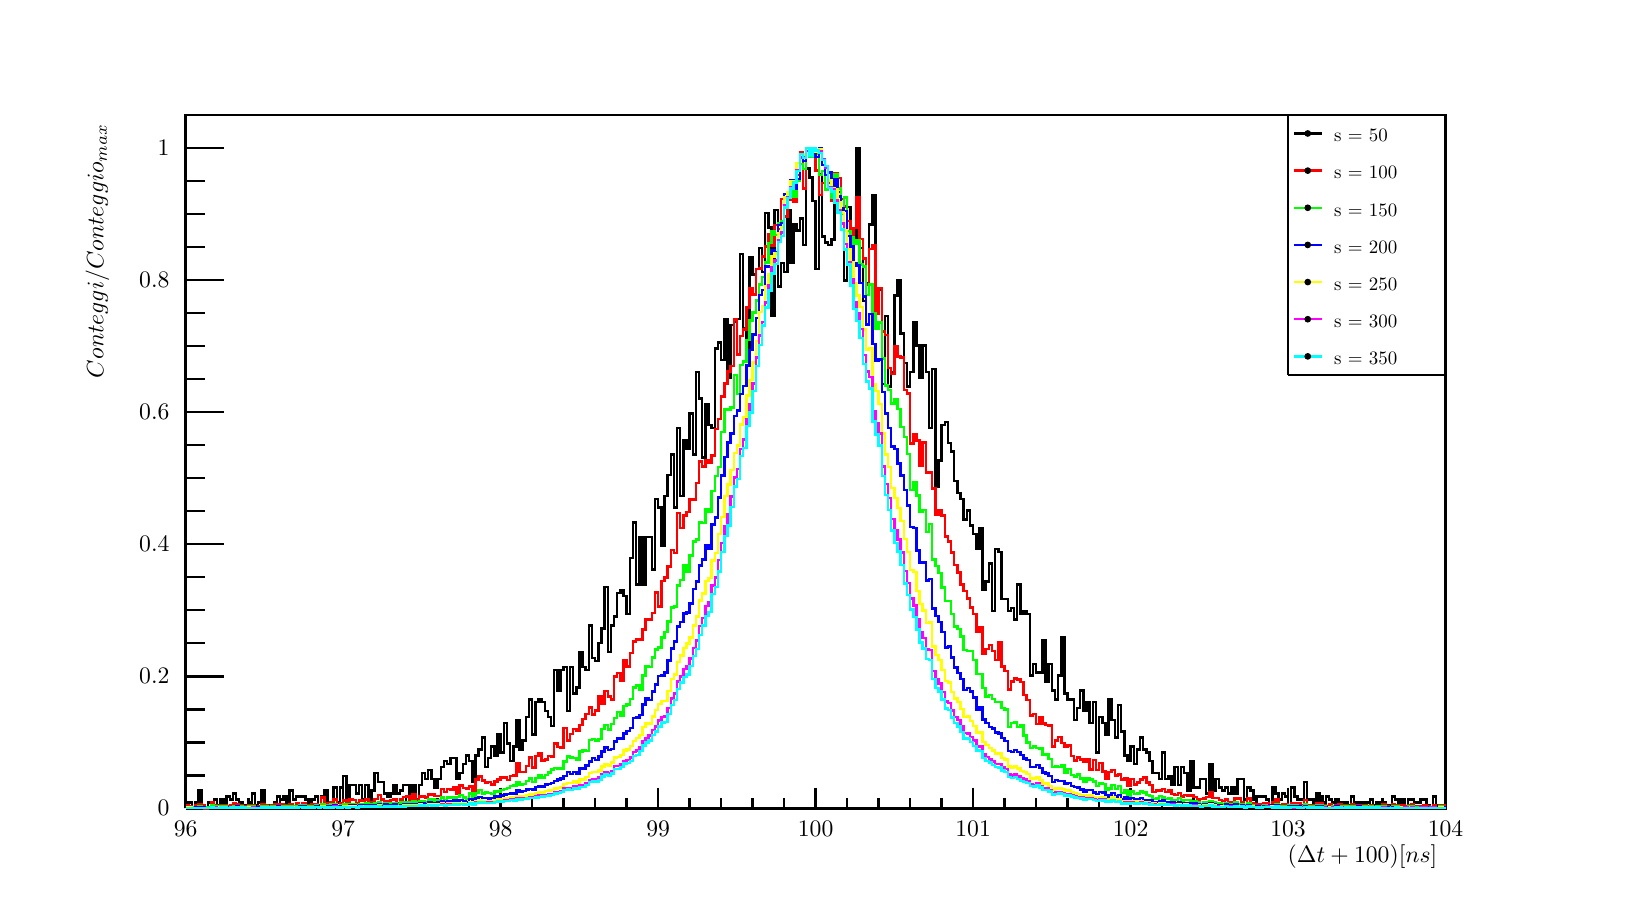
\begin{tikzpicture}
\pgfdeclareplotmark{cross} {
\pgfpathmoveto{\pgfpoint{-0.3\pgfplotmarksize}{\pgfplotmarksize}}
\pgfpathlineto{\pgfpoint{+0.3\pgfplotmarksize}{\pgfplotmarksize}}
\pgfpathlineto{\pgfpoint{+0.3\pgfplotmarksize}{0.3\pgfplotmarksize}}
\pgfpathlineto{\pgfpoint{+1\pgfplotmarksize}{0.3\pgfplotmarksize}}
\pgfpathlineto{\pgfpoint{+1\pgfplotmarksize}{-0.3\pgfplotmarksize}}
\pgfpathlineto{\pgfpoint{+0.3\pgfplotmarksize}{-0.3\pgfplotmarksize}}
\pgfpathlineto{\pgfpoint{+0.3\pgfplotmarksize}{-1.\pgfplotmarksize}}
\pgfpathlineto{\pgfpoint{-0.3\pgfplotmarksize}{-1.\pgfplotmarksize}}
\pgfpathlineto{\pgfpoint{-0.3\pgfplotmarksize}{-0.3\pgfplotmarksize}}
\pgfpathlineto{\pgfpoint{-1.\pgfplotmarksize}{-0.3\pgfplotmarksize}}
\pgfpathlineto{\pgfpoint{-1.\pgfplotmarksize}{0.3\pgfplotmarksize}}
\pgfpathlineto{\pgfpoint{-0.3\pgfplotmarksize}{0.3\pgfplotmarksize}}
\pgfpathclose
\pgfusepathqstroke
}
\pgfdeclareplotmark{cross*} {
\pgfpathmoveto{\pgfpoint{-0.3\pgfplotmarksize}{\pgfplotmarksize}}
\pgfpathlineto{\pgfpoint{+0.3\pgfplotmarksize}{\pgfplotmarksize}}
\pgfpathlineto{\pgfpoint{+0.3\pgfplotmarksize}{0.3\pgfplotmarksize}}
\pgfpathlineto{\pgfpoint{+1\pgfplotmarksize}{0.3\pgfplotmarksize}}
\pgfpathlineto{\pgfpoint{+1\pgfplotmarksize}{-0.3\pgfplotmarksize}}
\pgfpathlineto{\pgfpoint{+0.3\pgfplotmarksize}{-0.3\pgfplotmarksize}}
\pgfpathlineto{\pgfpoint{+0.3\pgfplotmarksize}{-1.\pgfplotmarksize}}
\pgfpathlineto{\pgfpoint{-0.3\pgfplotmarksize}{-1.\pgfplotmarksize}}
\pgfpathlineto{\pgfpoint{-0.3\pgfplotmarksize}{-0.3\pgfplotmarksize}}
\pgfpathlineto{\pgfpoint{-1.\pgfplotmarksize}{-0.3\pgfplotmarksize}}
\pgfpathlineto{\pgfpoint{-1.\pgfplotmarksize}{0.3\pgfplotmarksize}}
\pgfpathlineto{\pgfpoint{-0.3\pgfplotmarksize}{0.3\pgfplotmarksize}}
\pgfpathclose
\pgfusepathqfillstroke
}
\pgfdeclareplotmark{newstar} {
\pgfpathmoveto{\pgfqpoint{0pt}{\pgfplotmarksize}}
\pgfpathlineto{\pgfqpointpolar{44}{0.5\pgfplotmarksize}}
\pgfpathlineto{\pgfqpointpolar{18}{\pgfplotmarksize}}
\pgfpathlineto{\pgfqpointpolar{-20}{0.5\pgfplotmarksize}}
\pgfpathlineto{\pgfqpointpolar{-54}{\pgfplotmarksize}}
\pgfpathlineto{\pgfqpointpolar{-90}{0.5\pgfplotmarksize}}
\pgfpathlineto{\pgfqpointpolar{234}{\pgfplotmarksize}}
\pgfpathlineto{\pgfqpointpolar{198}{0.5\pgfplotmarksize}}
\pgfpathlineto{\pgfqpointpolar{162}{\pgfplotmarksize}}
\pgfpathlineto{\pgfqpointpolar{134}{0.5\pgfplotmarksize}}
\pgfpathclose
\pgfusepathqstroke
}
\pgfdeclareplotmark{newstar*} {
\pgfpathmoveto{\pgfqpoint{0pt}{\pgfplotmarksize}}
\pgfpathlineto{\pgfqpointpolar{44}{0.5\pgfplotmarksize}}
\pgfpathlineto{\pgfqpointpolar{18}{\pgfplotmarksize}}
\pgfpathlineto{\pgfqpointpolar{-20}{0.5\pgfplotmarksize}}
\pgfpathlineto{\pgfqpointpolar{-54}{\pgfplotmarksize}}
\pgfpathlineto{\pgfqpointpolar{-90}{0.5\pgfplotmarksize}}
\pgfpathlineto{\pgfqpointpolar{234}{\pgfplotmarksize}}
\pgfpathlineto{\pgfqpointpolar{198}{0.5\pgfplotmarksize}}
\pgfpathlineto{\pgfqpointpolar{162}{\pgfplotmarksize}}
\pgfpathlineto{\pgfqpointpolar{134}{0.5\pgfplotmarksize}}
\pgfpathclose
\pgfusepathqfillstroke
}
\definecolor{c}{rgb}{1,1,1};
\draw [color=c, fill=c] (0,0) rectangle (20,11.0085);
\draw [color=c, fill=c] (2,1.10085) rectangle (18,9.90762);
\definecolor{c}{rgb}{0,0,0};
\draw [c,line width=0.9] (2,1.10085) -- (2,9.90762) -- (18,9.90762) -- (18,1.10085) -- (2,1.10085);
\definecolor{c}{rgb}{1,1,1};
\draw [color=c, fill=c] (2,1.10085) rectangle (18,9.90762);
\definecolor{c}{rgb}{0,0,0};
\draw [c,line width=0.9] (2,1.10085) -- (2,9.90762) -- (18,9.90762) -- (18,1.10085) -- (2,1.10085);
\draw [c,line width=0.9] (2,1.17573) -- (2.04,1.17573) -- (2.04,1.17573) -- (2.08,1.17573) -- (2.08,1.10085) -- (2.12,1.10085) -- (2.12,1.17573) -- (2.16,1.17573) -- (2.16,1.32551) -- (2.2,1.32551) -- (2.2,1.13829) -- (2.24,1.13829) -- (2.24,1.10085)
 -- (2.28,1.10085) -- (2.28,1.17573) -- (2.32,1.17573) -- (2.32,1.17573) -- (2.36,1.17573) -- (2.36,1.21318) -- (2.4,1.21318) -- (2.4,1.13829) -- (2.44,1.13829) -- (2.44,1.21318) -- (2.48,1.21318) -- (2.48,1.17573) -- (2.52,1.17573) -- (2.52,1.25062)
 -- (2.56,1.25062) -- (2.56,1.21318) -- (2.6,1.21318) -- (2.6,1.28807) -- (2.64,1.28807) -- (2.64,1.21318) -- (2.68,1.21318) -- (2.68,1.17573) -- (2.72,1.17573) -- (2.72,1.13829) -- (2.76,1.13829) -- (2.76,1.13829) -- (2.8,1.13829) -- (2.8,1.17573)
 -- (2.84,1.17573) -- (2.84,1.28807) -- (2.88,1.28807) -- (2.88,1.13829) -- (2.92,1.13829) -- (2.92,1.17573) -- (2.96,1.17573) -- (2.96,1.32551) -- (3,1.32551) -- (3,1.13829) -- (3.04,1.13829) -- (3.04,1.13829) -- (3.08,1.13829) -- (3.08,1.13829) --
 (3.12,1.13829) -- (3.12,1.17573) -- (3.16,1.17573) -- (3.16,1.25062) -- (3.2,1.25062) -- (3.2,1.21318) -- (3.24,1.21318) -- (3.24,1.25062) -- (3.28,1.25062) -- (3.28,1.13829) -- (3.32,1.13829) -- (3.32,1.32551) -- (3.36,1.32551) -- (3.36,1.21318) --
 (3.4,1.21318) -- (3.4,1.25062) -- (3.44,1.25062) -- (3.44,1.25062) -- (3.48,1.25062) -- (3.48,1.25062) -- (3.52,1.25062) -- (3.52,1.21318) -- (3.56,1.21318) -- (3.56,1.17573) -- (3.6,1.17573) -- (3.6,1.21318) -- (3.64,1.21318) -- (3.64,1.25062) --
 (3.68,1.25062) -- (3.68,1.13829) -- (3.72,1.13829) -- (3.72,1.25062) -- (3.76,1.25062) -- (3.76,1.32551) -- (3.8,1.32551) -- (3.8,1.17573) -- (3.84,1.17573) -- (3.84,1.17573) -- (3.88,1.17573) -- (3.88,1.36295) -- (3.92,1.36295) -- (3.92,1.17573) --
 (3.96,1.17573) -- (3.96,1.36295) -- (4,1.36295) -- (4,1.51273) -- (4.04,1.51273) -- (4.04,1.13829) -- (4.08,1.13829) -- (4.08,1.4004) -- (4.12,1.4004) -- (4.12,1.4004) -- (4.16,1.4004) -- (4.16,1.28807) -- (4.2,1.28807) -- (4.2,1.4004) --
 (4.24,1.4004) -- (4.24,1.21318) -- (4.28,1.21318) -- (4.28,1.4004) -- (4.32,1.4004) -- (4.32,1.21318) -- (4.36,1.21318) -- (4.36,1.32551) -- (4.4,1.32551) -- (4.4,1.55017) -- (4.44,1.55017) -- (4.44,1.43784) -- (4.48,1.43784) -- (4.48,1.43784) --
 (4.52,1.43784) -- (4.52,1.28807) -- (4.56,1.28807) -- (4.56,1.25062) -- (4.6,1.25062) -- (4.6,1.28807) -- (4.64,1.28807) -- (4.64,1.4004) -- (4.68,1.4004) -- (4.68,1.28807) -- (4.72,1.28807) -- (4.72,1.32551) -- (4.76,1.32551) -- (4.76,1.4004) --
 (4.8,1.4004) -- (4.8,1.4004) -- (4.84,1.4004) -- (4.84,1.25062) -- (4.88,1.25062) -- (4.88,1.4004) -- (4.92,1.4004) -- (4.92,1.21318) -- (4.96,1.21318) -- (4.96,1.4004) -- (5,1.4004) -- (5,1.55017) -- (5.04,1.55017) -- (5.04,1.47528) --
 (5.08,1.47528) -- (5.08,1.58762) -- (5.12,1.58762) -- (5.12,1.47528) -- (5.16,1.47528) -- (5.16,1.36295) -- (5.2,1.36295) -- (5.2,1.47528) -- (5.24,1.47528) -- (5.24,1.62506) -- (5.28,1.62506) -- (5.28,1.69995) -- (5.32,1.69995) -- (5.32,1.6625) --
 (5.36,1.6625) -- (5.36,1.73739) -- (5.4,1.73739) -- (5.4,1.73739) -- (5.44,1.73739) -- (5.44,1.47528) -- (5.48,1.47528) -- (5.48,1.55017) -- (5.52,1.55017) -- (5.52,1.6625) -- (5.56,1.6625) -- (5.56,1.77483) -- (5.6,1.77483) -- (5.6,1.69995) --
 (5.64,1.69995) -- (5.64,1.43784) -- (5.68,1.43784) -- (5.68,1.77483) -- (5.72,1.77483) -- (5.72,1.84972) -- (5.76,1.84972) -- (5.76,1.9995) -- (5.8,1.9995) -- (5.8,1.62506) -- (5.84,1.62506) -- (5.84,1.73739) -- (5.88,1.73739) -- (5.88,1.88717) --
 (5.92,1.88717) -- (5.92,1.77483) -- (5.96,1.77483) -- (5.96,2.03694) -- (6,2.03694) -- (6,1.81228) -- (6.04,1.81228) -- (6.04,2.18672) -- (6.08,2.18672) -- (6.08,1.92461) -- (6.12,1.92461) -- (6.12,1.69995) -- (6.16,1.69995) -- (6.16,1.88717) --
 (6.2,1.88717) -- (6.2,2.22416) -- (6.24,2.22416) -- (6.24,1.84972) -- (6.28,1.84972) -- (6.28,1.96205) -- (6.32,1.96205) -- (6.32,2.2616) -- (6.36,2.2616) -- (6.36,2.48627) -- (6.4,2.48627) -- (6.4,2.03694) -- (6.44,2.03694) -- (6.44,2.44882) --
 (6.48,2.44882) -- (6.48,2.48627) -- (6.52,2.48627) -- (6.52,2.44882) -- (6.56,2.44882) -- (6.56,2.33649) -- (6.6,2.33649) -- (6.6,2.2616) -- (6.64,2.2616) -- (6.64,2.14927) -- (6.68,2.14927) -- (6.68,2.8607) -- (6.72,2.8607) -- (6.72,2.5986) --
 (6.76,2.5986) -- (6.76,2.8607) -- (6.8,2.8607) -- (6.8,2.89815) -- (6.84,2.89815) -- (6.84,2.33649) -- (6.88,2.33649) -- (6.88,2.89815) -- (6.92,2.89815) -- (6.92,2.56115) -- (6.96,2.56115) -- (6.96,2.63604) -- (7,2.63604) -- (7,3.08537) --
 (7.04,3.08537) -- (7.04,2.89815) -- (7.08,2.89815) -- (7.08,2.8607) -- (7.12,2.8607) -- (7.12,3.42236) -- (7.16,3.42236) -- (7.16,3.01048) -- (7.2,3.01048) -- (7.2,2.97304) -- (7.24,2.97304) -- (7.24,3.1977) -- (7.28,3.1977) -- (7.28,3.38492) --
 (7.32,3.38492) -- (7.32,3.90913) -- (7.36,3.90913) -- (7.36,3.08537) -- (7.4,3.08537) -- (7.4,3.42236) -- (7.44,3.42236) -- (7.44,3.53469) -- (7.48,3.53469) -- (7.48,3.83424) -- (7.52,3.83424) -- (7.52,3.87169) -- (7.56,3.87169) -- (7.56,3.7968) --
 (7.6,3.7968) -- (7.6,3.57214) -- (7.64,3.57214) -- (7.64,4.28357) -- (7.68,4.28357) -- (7.68,4.73289) -- (7.72,4.73289) -- (7.72,3.94657) -- (7.76,3.94657) -- (7.76,4.54567) -- (7.8,4.54567) -- (7.8,3.94657) -- (7.84,3.94657) -- (7.84,4.54567) --
 (7.88,4.54567) -- (7.88,4.54567) -- (7.92,4.54567) -- (7.92,4.13379) -- (7.96,4.13379) -- (7.96,5.03244) -- (8,5.03244) -- (8,4.92011) -- (8.04,4.92011) -- (8.04,4.43334) -- (8.08,4.43334) -- (8.08,5.06989) -- (8.12,5.06989) -- (8.12,5.33199) --
 (8.16,5.33199) -- (8.16,5.5941) -- (8.2,5.5941) -- (8.2,4.92011) -- (8.24,4.92011) -- (8.24,5.93109) -- (8.28,5.93109) -- (8.28,5.06989) -- (8.32,5.06989) -- (8.32,5.78132) -- (8.36,5.78132) -- (8.36,5.66899) -- (8.4,5.66899) -- (8.4,6.11831) --
 (8.44,6.11831) -- (8.44,5.5941) -- (8.48,5.5941) -- (8.48,6.64252) -- (8.52,6.64252) -- (8.52,6.30553) -- (8.56,6.30553) -- (8.56,5.55665) -- (8.6,5.55665) -- (8.6,6.23064) -- (8.64,6.23064) -- (8.64,5.96854) -- (8.68,5.96854) -- (8.68,5.93109) --
 (8.72,5.93109) -- (8.72,6.94207) -- (8.76,6.94207) -- (8.76,7.01696) -- (8.8,7.01696) -- (8.8,6.7923) -- (8.84,6.7923) -- (8.84,7.31651) -- (8.88,7.31651) -- (8.88,6.56764) -- (8.92,6.56764) -- (8.92,7.24162) -- (8.96,7.24162) -- (8.96,7.27907) --
 (9,7.27907) -- (9,7.31651) -- (9.04,7.31651) -- (9.04,8.14028) -- (9.08,8.14028) -- (9.08,7.20418) -- (9.12,7.20418) -- (9.12,6.86719) -- (9.16,6.86719) -- (9.16,8.10283) -- (9.2,8.10283) -- (9.2,7.87817) -- (9.24,7.87817) -- (9.24,7.95306) --
 (9.28,7.95306) -- (9.28,8.21516) -- (9.32,8.21516) -- (9.32,7.91561) -- (9.36,7.91561) -- (9.36,8.66449) -- (9.4,8.66449) -- (9.4,8.47727) -- (9.44,8.47727) -- (9.44,7.35396) -- (9.48,7.35396) -- (9.48,8.70193) -- (9.52,8.70193) -- (9.52,7.72839) --
 (9.56,7.72839) -- (9.56,8.02794) -- (9.6,8.02794) -- (9.6,7.91561) -- (9.64,7.91561) -- (9.64,8.70193) -- (9.68,8.70193) -- (9.68,8.02794) -- (9.72,8.02794) -- (9.72,8.51471) -- (9.76,8.51471) -- (9.76,8.43983) -- (9.8,8.43983) -- (9.8,8.5896) --
 (9.84,8.5896) -- (9.84,8.25261) -- (9.88,8.25261) -- (9.88,9.22614) -- (9.92,9.22614) -- (9.92,9.11381) -- (9.96,9.11381) -- (9.96,8.81426) -- (10,8.81426) -- (10,7.95306) -- (10.04,7.95306) -- (10.04,9.15126) -- (10.08,9.15126) -- (10.08,8.36494)
 -- (10.12,8.36494) -- (10.12,8.29005) -- (10.16,8.29005) -- (10.16,8.25261) -- (10.2,8.25261) -- (10.2,8.32749) -- (10.24,8.32749) -- (10.24,8.88915) -- (10.28,8.88915) -- (10.28,8.92659) -- (10.32,8.92659) -- (10.32,8.70193) -- (10.36,8.70193) --
 (10.36,7.80328) -- (10.4,7.80328) -- (10.4,8.73938) -- (10.44,8.73938) -- (10.44,8.06539) -- (10.48,8.06539) -- (10.48,8.29005) -- (10.52,8.29005) -- (10.52,9.48825) -- (10.56,9.48825) -- (10.56,8.21516) -- (10.6,8.21516) -- (10.6,7.54117) --
 (10.64,7.54117) -- (10.64,7.76584) -- (10.68,7.76584) -- (10.68,8.51471) -- (10.72,8.51471) -- (10.72,8.88915) -- (10.76,8.88915) -- (10.76,7.46629) -- (10.8,7.46629) -- (10.8,7.69095) -- (10.84,7.69095) -- (10.84,6.49275) -- (10.88,6.49275) --
 (10.88,7.35396) -- (10.92,7.35396) -- (10.92,6.45531) -- (10.96,6.45531) -- (10.96,6.64252) -- (11,6.64252) -- (11,7.61606) -- (11.04,7.61606) -- (11.04,7.80328) -- (11.08,7.80328) -- (11.08,7.12929) -- (11.12,7.12929) -- (11.12,6.75486) --
 (11.16,6.75486) -- (11.16,6.45531) -- (11.2,6.45531) -- (11.2,6.64252) -- (11.24,6.64252) -- (11.24,7.27907) -- (11.28,7.27907) -- (11.28,6.97952) -- (11.32,6.97952) -- (11.32,6.56764) -- (11.36,6.56764) -- (11.36,6.97952) -- (11.4,6.97952) --
 (11.4,6.64252) -- (11.44,6.64252) -- (11.44,5.93109) -- (11.48,5.93109) -- (11.48,6.67997) -- (11.52,6.67997) -- (11.52,5.18222) -- (11.56,5.18222) -- (11.56,5.51921) -- (11.6,5.51921) -- (11.6,5.96854) -- (11.64,5.96854) -- (11.64,6.00598) --
 (11.68,6.00598) -- (11.68,5.74387) -- (11.72,5.74387) -- (11.72,5.63154) -- (11.76,5.63154) -- (11.76,5.2571) -- (11.8,5.2571) -- (11.8,5.10733) -- (11.84,5.10733) -- (11.84,5.03244) -- (11.88,5.03244) -- (11.88,4.77034) -- (11.92,4.77034) --
 (11.92,4.88267) -- (11.96,4.88267) -- (11.96,4.69545) -- (12,4.69545) -- (12,4.58312) -- (12.04,4.58312) -- (12.04,4.3959) -- (12.08,4.3959) -- (12.08,4.658) -- (12.12,4.658) -- (12.12,3.87169) -- (12.16,3.87169) -- (12.16,3.98402) -- (12.2,3.98402)
 -- (12.2,4.20868) -- (12.24,4.20868) -- (12.24,3.60958) -- (12.28,3.60958) -- (12.28,4.3959) -- (12.32,4.3959) -- (12.32,4.35845) -- (12.36,4.35845) -- (12.36,3.75935) -- (12.4,3.75935) -- (12.4,3.75935) -- (12.44,3.75935) -- (12.44,3.60958) --
 (12.48,3.60958) -- (12.48,3.64702) -- (12.52,3.64702) -- (12.52,3.49725) -- (12.56,3.49725) -- (12.56,3.94657) -- (12.6,3.94657) -- (12.6,3.57214) -- (12.64,3.57214) -- (12.64,3.60958) -- (12.68,3.60958) -- (12.68,3.57214) -- (12.72,3.57214) --
 (12.72,2.78582) -- (12.76,2.78582) -- (12.76,2.93559) -- (12.8,2.93559) -- (12.8,2.82326) -- (12.84,2.82326) -- (12.84,2.82326) -- (12.88,2.82326) -- (12.88,3.23514) -- (12.92,3.23514) -- (12.92,2.71093) -- (12.96,2.71093) -- (12.96,2.93559) --
 (13,2.93559) -- (13,2.5986) -- (13.04,2.5986) -- (13.04,2.48627) -- (13.08,2.48627) -- (13.08,2.78582) -- (13.12,2.78582) -- (13.12,3.27259) -- (13.16,3.27259) -- (13.16,2.56115) -- (13.2,2.56115) -- (13.2,2.48627) -- (13.24,2.48627) --
 (13.24,2.48627) -- (13.28,2.48627) -- (13.28,2.22416) -- (13.32,2.22416) -- (13.32,2.37393) -- (13.36,2.37393) -- (13.36,2.5986) -- (13.4,2.5986) -- (13.4,2.33649) -- (13.44,2.33649) -- (13.44,2.44882) -- (13.48,2.44882) -- (13.48,2.18672) --
 (13.52,2.18672) -- (13.52,2.44882) -- (13.56,2.44882) -- (13.56,1.81228) -- (13.6,1.81228) -- (13.6,2.2616) -- (13.64,2.2616) -- (13.64,2.18672) -- (13.68,2.18672) -- (13.68,2.03694) -- (13.72,2.03694) -- (13.72,2.48627) -- (13.76,2.48627) --
 (13.76,2.22416) -- (13.8,2.22416) -- (13.8,1.9995) -- (13.84,1.9995) -- (13.84,2.41138) -- (13.88,2.41138) -- (13.88,2.07438) -- (13.92,2.07438) -- (13.92,1.77483) -- (13.96,1.77483) -- (13.96,1.69995) -- (14,1.69995) -- (14,1.88717) --
 (14.04,1.88717) -- (14.04,1.6625) -- (14.08,1.6625) -- (14.08,1.84972) -- (14.12,1.84972) -- (14.12,1.9995) -- (14.16,1.9995) -- (14.16,1.84972) -- (14.2,1.84972) -- (14.2,1.81228) -- (14.24,1.81228) -- (14.24,1.69995) -- (14.28,1.69995) --
 (14.28,1.55017) -- (14.32,1.55017) -- (14.32,1.55017) -- (14.36,1.55017) -- (14.36,1.47528) -- (14.4,1.47528) -- (14.4,1.81228) -- (14.44,1.81228) -- (14.44,1.47528) -- (14.48,1.47528) -- (14.48,1.51273) -- (14.52,1.51273) -- (14.52,1.4004) --
 (14.56,1.4004) -- (14.56,1.62506) -- (14.6,1.62506) -- (14.6,1.4004) -- (14.64,1.4004) -- (14.64,1.62506) -- (14.68,1.62506) -- (14.68,1.55017) -- (14.72,1.55017) -- (14.72,1.32551) -- (14.76,1.32551) -- (14.76,1.69995) -- (14.8,1.69995) --
 (14.8,1.36295) -- (14.84,1.36295) -- (14.84,1.36295) -- (14.88,1.36295) -- (14.88,1.47528) -- (14.92,1.47528) -- (14.92,1.47528) -- (14.96,1.47528) -- (14.96,1.28807) -- (15,1.28807) -- (15,1.6625) -- (15.04,1.6625) -- (15.04,1.32551) --
 (15.08,1.32551) -- (15.08,1.47528) -- (15.12,1.47528) -- (15.12,1.36295) -- (15.16,1.36295) -- (15.16,1.32551) -- (15.2,1.32551) -- (15.2,1.36295) -- (15.24,1.36295) -- (15.24,1.28807) -- (15.28,1.28807) -- (15.28,1.36295) -- (15.32,1.36295) --
 (15.32,1.28807) -- (15.36,1.28807) -- (15.36,1.47528) -- (15.4,1.47528) -- (15.4,1.47528) -- (15.44,1.47528) -- (15.44,1.21318) -- (15.48,1.21318) -- (15.48,1.36295) -- (15.52,1.36295) -- (15.52,1.32551) -- (15.56,1.32551) -- (15.56,1.21318) --
 (15.6,1.21318) -- (15.6,1.25062) -- (15.64,1.25062) -- (15.64,1.25062) -- (15.68,1.25062) -- (15.68,1.25062) -- (15.72,1.25062) -- (15.72,1.21318) -- (15.76,1.21318) -- (15.76,1.13829) -- (15.8,1.13829) -- (15.8,1.36295) -- (15.84,1.36295) --
 (15.84,1.28807) -- (15.88,1.28807) -- (15.88,1.21318) -- (15.92,1.21318) -- (15.92,1.28807) -- (15.96,1.28807) -- (15.96,1.25062) -- (16,1.25062) -- (16,1.13829) -- (16.04,1.13829) -- (16.04,1.36295) -- (16.08,1.36295) -- (16.08,1.25062) --
 (16.12,1.25062) -- (16.12,1.21318) -- (16.16,1.21318) -- (16.16,1.21318) -- (16.2,1.21318) -- (16.2,1.43784) -- (16.24,1.43784) -- (16.24,1.21318) -- (16.28,1.21318) -- (16.28,1.21318) -- (16.32,1.21318) -- (16.32,1.13829) -- (16.36,1.13829) --
 (16.36,1.28807) -- (16.4,1.28807) -- (16.4,1.25062) -- (16.44,1.25062) -- (16.44,1.17573) -- (16.48,1.17573) -- (16.48,1.25062) -- (16.52,1.25062) -- (16.52,1.21318) -- (16.56,1.21318) -- (16.56,1.17573) -- (16.6,1.17573) -- (16.6,1.21318) --
 (16.64,1.21318) -- (16.64,1.13829) -- (16.68,1.13829) -- (16.68,1.17573) -- (16.72,1.17573) -- (16.72,1.17573) -- (16.76,1.17573) -- (16.76,1.13829) -- (16.8,1.13829) -- (16.8,1.25062) -- (16.84,1.25062) -- (16.84,1.17573) -- (16.88,1.17573) --
 (16.88,1.17573) -- (16.92,1.17573) -- (16.92,1.17573) -- (16.96,1.17573) -- (16.96,1.17573) -- (17,1.17573) -- (17,1.17573) -- (17.04,1.17573) -- (17.04,1.21318) -- (17.08,1.21318) -- (17.08,1.13829) -- (17.12,1.13829) -- (17.12,1.17573) --
 (17.16,1.17573) -- (17.16,1.13829) -- (17.2,1.13829) -- (17.2,1.17573) -- (17.24,1.17573) -- (17.24,1.13829) -- (17.28,1.13829) -- (17.28,1.13829) -- (17.32,1.13829) -- (17.32,1.25062) -- (17.36,1.25062) -- (17.36,1.21318) -- (17.4,1.21318) --
 (17.4,1.13829) -- (17.44,1.13829) -- (17.44,1.21318) -- (17.48,1.21318) -- (17.48,1.10085) -- (17.52,1.10085) -- (17.52,1.21318) -- (17.56,1.21318) -- (17.56,1.21318) -- (17.6,1.21318) -- (17.6,1.17573) -- (17.64,1.17573) -- (17.64,1.17573) --
 (17.68,1.17573) -- (17.68,1.21318) -- (17.72,1.21318) -- (17.72,1.21318) -- (17.76,1.21318) -- (17.76,1.13829) -- (17.8,1.13829) -- (17.8,1.10085) -- (17.84,1.10085) -- (17.84,1.25062) -- (17.88,1.25062) -- (17.88,1.13829) -- (17.92,1.13829) --
 (17.92,1.10085) -- (17.96,1.10085) -- (17.96,1.10085) -- (18,1.10085);
\draw [c,line width=0.9] (2,1.10085) -- (18,1.10085);
\draw [anchor= east] (18,0.484373) node[scale=0.854877, color=c, rotate=0]{$(\Delta t + 100) [ns]$};
\draw [c,line width=0.9] (2,1.36505) -- (2,1.10085);
\draw [c,line width=0.9] (2.4,1.23295) -- (2.4,1.10085);
\draw [c,line width=0.9] (2.8,1.23295) -- (2.8,1.10085);
\draw [c,line width=0.9] (3.2,1.23295) -- (3.2,1.10085);
\draw [c,line width=0.9] (3.6,1.23295) -- (3.6,1.10085);
\draw [c,line width=0.9] (4,1.36505) -- (4,1.10085);
\draw [c,line width=0.9] (4.4,1.23295) -- (4.4,1.10085);
\draw [c,line width=0.9] (4.8,1.23295) -- (4.8,1.10085);
\draw [c,line width=0.9] (5.2,1.23295) -- (5.2,1.10085);
\draw [c,line width=0.9] (5.6,1.23295) -- (5.6,1.10085);
\draw [c,line width=0.9] (6,1.36505) -- (6,1.10085);
\draw [c,line width=0.9] (6.4,1.23295) -- (6.4,1.10085);
\draw [c,line width=0.9] (6.8,1.23295) -- (6.8,1.10085);
\draw [c,line width=0.9] (7.2,1.23295) -- (7.2,1.10085);
\draw [c,line width=0.9] (7.6,1.23295) -- (7.6,1.10085);
\draw [c,line width=0.9] (8,1.36505) -- (8,1.10085);
\draw [c,line width=0.9] (8.4,1.23295) -- (8.4,1.10085);
\draw [c,line width=0.9] (8.8,1.23295) -- (8.8,1.10085);
\draw [c,line width=0.9] (9.2,1.23295) -- (9.2,1.10085);
\draw [c,line width=0.9] (9.6,1.23295) -- (9.6,1.10085);
\draw [c,line width=0.9] (10,1.36505) -- (10,1.10085);
\draw [c,line width=0.9] (10.4,1.23295) -- (10.4,1.10085);
\draw [c,line width=0.9] (10.8,1.23295) -- (10.8,1.10085);
\draw [c,line width=0.9] (11.2,1.23295) -- (11.2,1.10085);
\draw [c,line width=0.9] (11.6,1.23295) -- (11.6,1.10085);
\draw [c,line width=0.9] (12,1.36505) -- (12,1.10085);
\draw [c,line width=0.9] (12.4,1.23295) -- (12.4,1.10085);
\draw [c,line width=0.9] (12.8,1.23295) -- (12.8,1.10085);
\draw [c,line width=0.9] (13.2,1.23295) -- (13.2,1.10085);
\draw [c,line width=0.9] (13.6,1.23295) -- (13.6,1.10085);
\draw [c,line width=0.9] (14,1.36505) -- (14,1.10085);
\draw [c,line width=0.9] (14.4,1.23295) -- (14.4,1.10085);
\draw [c,line width=0.9] (14.8,1.23295) -- (14.8,1.10085);
\draw [c,line width=0.9] (15.2,1.23295) -- (15.2,1.10085);
\draw [c,line width=0.9] (15.6,1.23295) -- (15.6,1.10085);
\draw [c,line width=0.9] (16,1.36505) -- (16,1.10085);
\draw [c,line width=0.9] (16.4,1.23295) -- (16.4,1.10085);
\draw [c,line width=0.9] (16.8,1.23295) -- (16.8,1.10085);
\draw [c,line width=0.9] (17.2,1.23295) -- (17.2,1.10085);
\draw [c,line width=0.9] (17.6,1.23295) -- (17.6,1.10085);
\draw [c,line width=0.9] (18,1.36505) -- (18,1.10085);
\draw [anchor=base] (2,0.737567) node[scale=0.854877, color=c, rotate=0]{96};
\draw [anchor=base] (4,0.737567) node[scale=0.854877, color=c, rotate=0]{97};
\draw [anchor=base] (6,0.737567) node[scale=0.854877, color=c, rotate=0]{98};
\draw [anchor=base] (8,0.737567) node[scale=0.854877, color=c, rotate=0]{99};
\draw [anchor=base] (10,0.737567) node[scale=0.854877, color=c, rotate=0]{100};
\draw [anchor=base] (12,0.737567) node[scale=0.854877, color=c, rotate=0]{101};
\draw [anchor=base] (14,0.737567) node[scale=0.854877, color=c, rotate=0]{102};
\draw [anchor=base] (16,0.737567) node[scale=0.854877, color=c, rotate=0]{103};
\draw [anchor=base] (18,0.737567) node[scale=0.854877, color=c, rotate=0]{104};
\draw [c,line width=0.9] (2,1.10085) -- (2,9.90762);
\draw [anchor= east] (0.88,9.90762) node[scale=0.854877, color=c, rotate=90]{$Conteggi/Conteggio_{max}$};
\draw [c,line width=0.9] (2.48,1.10085) -- (2,1.10085);
\draw [c,line width=0.9] (2.24,1.52022) -- (2,1.52022);
\draw [c,line width=0.9] (2.24,1.93959) -- (2,1.93959);
\draw [c,line width=0.9] (2.24,2.35896) -- (2,2.35896);
\draw [c,line width=0.9] (2.48,2.77833) -- (2,2.77833);
\draw [c,line width=0.9] (2.24,3.1977) -- (2,3.1977);
\draw [c,line width=0.9] (2.24,3.61707) -- (2,3.61707);
\draw [c,line width=0.9] (2.24,4.03644) -- (2,4.03644);
\draw [c,line width=0.9] (2.48,4.45581) -- (2,4.45581);
\draw [c,line width=0.9] (2.24,4.87518) -- (2,4.87518);
\draw [c,line width=0.9] (2.24,5.29455) -- (2,5.29455);
\draw [c,line width=0.9] (2.24,5.71392) -- (2,5.71392);
\draw [c,line width=0.9] (2.48,6.13329) -- (2,6.13329);
\draw [c,line width=0.9] (2.24,6.55266) -- (2,6.55266);
\draw [c,line width=0.9] (2.24,6.97203) -- (2,6.97203);
\draw [c,line width=0.9] (2.24,7.3914) -- (2,7.3914);
\draw [c,line width=0.9] (2.48,7.81077) -- (2,7.81077);
\draw [c,line width=0.9] (2.24,8.23014) -- (2,8.23014);
\draw [c,line width=0.9] (2.24,8.64951) -- (2,8.64951);
\draw [c,line width=0.9] (2.24,9.06888) -- (2,9.06888);
\draw [c,line width=0.9] (2.48,9.48825) -- (2,9.48825);
\draw [c,line width=0.9] (2.48,9.48825) -- (2,9.48825);
\draw [anchor= east] (1.9,1.10085) node[scale=0.854877, color=c, rotate=0]{0};
\draw [anchor= east] (1.9,2.77833) node[scale=0.854877, color=c, rotate=0]{0.2};
\draw [anchor= east] (1.9,4.45581) node[scale=0.854877, color=c, rotate=0]{0.4};
\draw [anchor= east] (1.9,6.13329) node[scale=0.854877, color=c, rotate=0]{0.6};
\draw [anchor= east] (1.9,7.81077) node[scale=0.854877, color=c, rotate=0]{0.8};
\draw [anchor= east] (1.9,9.48825) node[scale=0.854877, color=c, rotate=0]{1};
\definecolor{c}{rgb}{1,0,0};
\draw [c,line width=0.9] (2,1.13562) -- (2.04,1.13562) -- (2.04,1.12171) -- (2.08,1.12171) -- (2.08,1.1078) -- (2.12,1.1078) -- (2.12,1.13562) -- (2.16,1.13562) -- (2.16,1.14953) -- (2.2,1.14953) -- (2.2,1.13562) -- (2.24,1.13562) -- (2.24,1.10085)
 -- (2.28,1.10085) -- (2.28,1.11476) -- (2.32,1.11476) -- (2.32,1.17735) -- (2.36,1.17735) -- (2.36,1.14258) -- (2.4,1.14258) -- (2.4,1.12867) -- (2.44,1.12867) -- (2.44,1.14258) -- (2.48,1.14258) -- (2.48,1.13562) -- (2.52,1.13562) -- (2.52,1.12867)
 -- (2.56,1.12867) -- (2.56,1.14258) -- (2.6,1.14258) -- (2.6,1.16344) -- (2.64,1.16344) -- (2.64,1.14953) -- (2.68,1.14953) -- (2.68,1.14258) -- (2.72,1.14258) -- (2.72,1.11476) -- (2.76,1.11476) -- (2.76,1.12171) -- (2.8,1.12171) -- (2.8,1.14258)
 -- (2.84,1.14258) -- (2.84,1.14258) -- (2.88,1.14258) -- (2.88,1.11476) -- (2.92,1.11476) -- (2.92,1.12171) -- (2.96,1.12171) -- (2.96,1.14953) -- (3,1.14953) -- (3,1.14258) -- (3.04,1.14258) -- (3.04,1.12867) -- (3.08,1.12867) -- (3.08,1.13562) --
 (3.12,1.13562) -- (3.12,1.14953) -- (3.16,1.14953) -- (3.16,1.14953) -- (3.2,1.14953) -- (3.2,1.14953) -- (3.24,1.14953) -- (3.24,1.13562) -- (3.28,1.13562) -- (3.28,1.12171) -- (3.32,1.12171) -- (3.32,1.14953) -- (3.36,1.14953) -- (3.36,1.12171) --
 (3.4,1.12171) -- (3.4,1.16344) -- (3.44,1.16344) -- (3.44,1.13562) -- (3.48,1.13562) -- (3.48,1.17039) -- (3.52,1.17039) -- (3.52,1.12867) -- (3.56,1.12867) -- (3.56,1.13562) -- (3.6,1.13562) -- (3.6,1.14953) -- (3.64,1.14953) -- (3.64,1.14953) --
 (3.68,1.14953) -- (3.68,1.11476) -- (3.72,1.11476) -- (3.72,1.23994) -- (3.76,1.23994) -- (3.76,1.16344) -- (3.8,1.16344) -- (3.8,1.14953) -- (3.84,1.14953) -- (3.84,1.1843) -- (3.88,1.1843) -- (3.88,1.21212) -- (3.92,1.21212) -- (3.92,1.12171) --
 (3.96,1.12171) -- (3.96,1.16344) -- (4,1.16344) -- (4,1.19821) -- (4.04,1.19821) -- (4.04,1.14258) -- (4.08,1.14258) -- (4.08,1.21212) -- (4.12,1.21212) -- (4.12,1.20517) -- (4.16,1.20517) -- (4.16,1.16344) -- (4.2,1.16344) -- (4.2,1.19821) --
 (4.24,1.19821) -- (4.24,1.19126) -- (4.28,1.19126) -- (4.28,1.21212) -- (4.32,1.21212) -- (4.32,1.17039) -- (4.36,1.17039) -- (4.36,1.1843) -- (4.4,1.1843) -- (4.4,1.21908) -- (4.44,1.21908) -- (4.44,1.26776) -- (4.48,1.26776) -- (4.48,1.21212) --
 (4.52,1.21212) -- (4.52,1.19126) -- (4.56,1.19126) -- (4.56,1.16344) -- (4.6,1.16344) -- (4.6,1.20517) -- (4.64,1.20517) -- (4.64,1.21212) -- (4.68,1.21212) -- (4.68,1.17039) -- (4.72,1.17039) -- (4.72,1.21212) -- (4.76,1.21212) -- (4.76,1.2469) --
 (4.8,1.2469) -- (4.8,1.25385) -- (4.84,1.25385) -- (4.84,1.21212) -- (4.88,1.21212) -- (4.88,1.27472) -- (4.92,1.27472) -- (4.92,1.19821) -- (4.96,1.19821) -- (4.96,1.25385) -- (5,1.25385) -- (5,1.25385) -- (5.04,1.25385) -- (5.04,1.23994) --
 (5.08,1.23994) -- (5.08,1.27472) -- (5.12,1.27472) -- (5.12,1.28167) -- (5.16,1.28167) -- (5.16,1.26081) -- (5.2,1.26081) -- (5.2,1.26081) -- (5.24,1.26081) -- (5.24,1.34426) -- (5.28,1.34426) -- (5.28,1.30949) -- (5.32,1.30949) -- (5.32,1.34426) --
 (5.36,1.34426) -- (5.36,1.33731) -- (5.4,1.33731) -- (5.4,1.36513) -- (5.44,1.36513) -- (5.44,1.28862) -- (5.48,1.28862) -- (5.48,1.39295) -- (5.52,1.39295) -- (5.52,1.35817) -- (5.56,1.35817) -- (5.56,1.35122) -- (5.6,1.35122) -- (5.6,1.37904) --
 (5.64,1.37904) -- (5.64,1.3234) -- (5.68,1.3234) -- (5.68,1.46945) -- (5.72,1.46945) -- (5.72,1.50422) -- (5.76,1.50422) -- (5.76,1.45554) -- (5.8,1.45554) -- (5.8,1.42772) -- (5.84,1.42772) -- (5.84,1.43467) -- (5.88,1.43467) -- (5.88,1.40685) --
 (5.92,1.40685) -- (5.92,1.44163) -- (5.96,1.44163) -- (5.96,1.46945) -- (6,1.46945) -- (6,1.49031) -- (6.04,1.49031) -- (6.04,1.49031) -- (6.08,1.49031) -- (6.08,1.46249) -- (6.12,1.46249) -- (6.12,1.51118) -- (6.16,1.51118) -- (6.16,1.51813) --
 (6.2,1.51813) -- (6.2,1.67809) -- (6.24,1.67809) -- (6.24,1.55986) -- (6.28,1.55986) -- (6.28,1.55986) -- (6.32,1.55986) -- (6.32,1.63636) -- (6.36,1.63636) -- (6.36,1.74764) -- (6.4,1.74764) -- (6.4,1.62245) -- (6.44,1.62245) -- (6.44,1.7685) --
 (6.48,1.7685) -- (6.48,1.80327) -- (6.52,1.80327) -- (6.52,1.70591) -- (6.56,1.70591) -- (6.56,1.71982) -- (6.6,1.71982) -- (6.6,1.7685) -- (6.64,1.7685) -- (6.64,1.76155) -- (6.68,1.76155) -- (6.68,1.9215) -- (6.72,1.9215) -- (6.72,1.87978) --
 (6.76,1.87978) -- (6.76,1.87282) -- (6.8,1.87282) -- (6.8,2.12319) -- (6.84,2.12319) -- (6.84,1.96323) -- (6.88,1.96323) -- (6.88,2.04669) -- (6.92,2.04669) -- (6.92,2.10928) -- (6.96,2.10928) -- (6.96,2.08146) -- (7,2.08146) -- (7,2.15797) --
 (7.04,2.15797) -- (7.04,2.23447) -- (7.08,2.23447) -- (7.08,2.29706) -- (7.12,2.29706) -- (7.12,2.38052) -- (7.16,2.38052) -- (7.16,2.29011) -- (7.2,2.29011) -- (7.2,2.34574) -- (7.24,2.34574) -- (7.24,2.52657) -- (7.28,2.52657) -- (7.28,2.4292) --
 (7.32,2.4292) -- (7.32,2.58916) -- (7.36,2.58916) -- (7.36,2.51961) -- (7.4,2.51961) -- (7.4,2.48484) -- (7.44,2.48484) -- (7.44,2.77694) -- (7.48,2.77694) -- (7.48,2.81867) -- (7.52,2.81867) -- (7.52,2.7213) -- (7.56,2.7213) -- (7.56,2.97862) --
 (7.6,2.97862) -- (7.6,2.90212) -- (7.64,2.90212) -- (7.64,3.07599) -- (7.68,3.07599) -- (7.68,3.22204) -- (7.72,3.22204) -- (7.72,3.2429) -- (7.76,3.2429) -- (7.76,3.23595) -- (7.8,3.23595) -- (7.8,3.37504) -- (7.84,3.37504) -- (7.84,3.50718) --
 (7.88,3.50718) -- (7.88,3.50023) -- (7.92,3.50023) -- (7.92,3.58369) -- (7.96,3.58369) -- (7.96,3.84101) -- (8,3.84101) -- (8,3.66714) -- (8.04,3.66714) -- (8.04,3.98706) -- (8.08,3.98706) -- (8.08,4.03574) -- (8.12,4.03574) -- (8.12,4.17484) --
 (8.16,4.17484) -- (8.16,4.38348) -- (8.2,4.38348) -- (8.2,4.34175) -- (8.24,4.34175) -- (8.24,4.84945) -- (8.28,4.84945) -- (8.28,4.66167) -- (8.32,4.66167) -- (8.32,4.82163) -- (8.36,4.82163) -- (8.36,4.86336) -- (8.4,4.86336) -- (8.4,5.02331) --
 (8.44,5.02331) -- (8.44,5.02331) -- (8.48,5.02331) -- (8.48,5.23196) -- (8.52,5.23196) -- (8.52,5.50319) -- (8.56,5.50319) -- (8.56,5.4406) -- (8.6,5.4406) -- (8.6,5.5171) -- (8.64,5.5171) -- (8.64,5.48928) -- (8.68,5.48928) -- (8.68,5.57969) --
 (8.72,5.57969) -- (8.72,5.92047) -- (8.76,5.92047) -- (8.76,6.04566) -- (8.8,6.04566) -- (8.8,6.3308) -- (8.84,6.3308) -- (8.84,6.49772) -- (8.88,6.49772) -- (8.88,6.65072) -- (8.92,6.65072) -- (8.92,6.72027) -- (8.96,6.72027) -- (8.96,7.31142) --
 (9,7.31142) -- (9,6.86632) -- (9.04,6.86632) -- (9.04,7.10278) -- (9.08,7.10278) -- (9.08,7.17928) -- (9.12,7.17928) -- (9.12,7.46442) -- (9.16,7.46442) -- (9.16,7.70089) -- (9.2,7.70089) -- (9.2,7.62438) -- (9.24,7.62438) -- (9.24,7.95126) --
 (9.28,7.95126) -- (9.28,7.95821) -- (9.32,7.95821) -- (9.32,8.11121) -- (9.36,8.11121) -- (9.36,8.2364) -- (9.4,8.2364) -- (9.4,8.39636) -- (9.44,8.39636) -- (9.44,8.24335) -- (9.48,8.24335) -- (9.48,8.50763) -- (9.52,8.50763) -- (9.52,8.45895) --
 (9.56,8.45895) -- (9.56,8.84146) -- (9.6,8.84146) -- (9.6,8.61891) -- (9.64,8.61891) -- (9.64,8.82755) -- (9.68,8.82755) -- (9.68,8.95969) -- (9.72,8.95969) -- (9.72,8.80669) -- (9.76,8.80669) -- (9.76,9.14747) -- (9.8,9.14747) -- (9.8,9.43261) --
 (9.84,9.43261) -- (9.84,8.9736) -- (9.88,8.9736) -- (9.88,9.45348) -- (9.92,9.45348) -- (9.92,9.48825) -- (9.96,9.48825) -- (9.96,9.44652) -- (10,9.44652) -- (10,9.20311) -- (10.04,9.20311) -- (10.04,8.89014) -- (10.08,8.89014) -- (10.08,9.04315) --
 (10.12,9.04315) -- (10.12,9.14747) -- (10.16,9.14747) -- (10.16,9.04315) -- (10.2,9.04315) -- (10.2,8.81364) -- (10.24,8.81364) -- (10.24,9.16138) -- (10.28,9.16138) -- (10.28,9.10574) -- (10.32,9.10574) -- (10.32,8.84146) -- (10.36,8.84146) --
 (10.36,8.74409) -- (10.4,8.74409) -- (10.4,8.56327) -- (10.44,8.56327) -- (10.44,8.36854) -- (10.48,8.36854) -- (10.48,8.47286) -- (10.52,8.47286) -- (10.52,8.86232) -- (10.56,8.86232) -- (10.56,8.33377) -- (10.6,8.33377) -- (10.6,8.0834) --
 (10.64,8.0834) -- (10.64,7.75652) -- (10.68,7.75652) -- (10.68,8.20163) -- (10.72,8.20163) -- (10.72,8.25726) -- (10.76,8.25726) -- (10.76,7.38097) -- (10.8,7.38097) -- (10.8,7.70784) -- (10.84,7.70784) -- (10.84,7.15842) -- (10.88,7.15842) --
 (10.88,7.10973) -- (10.92,7.10973) -- (10.92,6.69245) -- (10.96,6.69245) -- (10.96,6.61595) -- (11,6.61595) -- (11,6.97064) -- (11.04,6.97064) -- (11.04,6.8385) -- (11.08,6.8385) -- (11.08,6.82459) -- (11.12,6.82459) -- (11.12,6.41426) --
 (11.16,6.41426) -- (11.16,6.37253) -- (11.2,6.37253) -- (11.2,5.7327) -- (11.24,5.7327) -- (11.24,5.85788) -- (11.28,5.85788) -- (11.28,5.77443) -- (11.32,5.77443) -- (11.32,5.45451) -- (11.36,5.45451) -- (11.36,5.74661) -- (11.4,5.74661) --
 (11.4,5.3641) -- (11.44,5.3641) -- (11.44,5.3641) -- (11.48,5.3641) -- (11.48,5.16241) -- (11.52,5.16241) -- (11.52,4.82858) -- (11.56,4.82858) -- (11.56,4.88422) -- (11.6,4.88422) -- (11.6,4.82163) -- (11.64,4.82163) -- (11.64,4.55039) --
 (11.68,4.55039) -- (11.68,4.4878) -- (11.72,4.4878) -- (11.72,4.34871) -- (11.76,4.34871) -- (11.76,4.18875) -- (11.8,4.18875) -- (11.8,4.09834) -- (11.84,4.09834) -- (11.84,3.94533) -- (11.88,3.94533) -- (11.88,3.86187) -- (11.92,3.86187) --
 (11.92,3.76451) -- (11.96,3.76451) -- (11.96,3.65323) -- (12,3.65323) -- (12,3.56978) -- (12.04,3.56978) -- (12.04,3.34027) -- (12.08,3.34027) -- (12.08,3.39591) -- (12.12,3.39591) -- (12.12,3.06904) -- (12.16,3.06904) -- (12.16,3.12467) --
 (12.2,3.12467) -- (12.2,3.17336) -- (12.24,3.17336) -- (12.24,3.09685) -- (12.28,3.09685) -- (12.28,2.98558) -- (12.32,2.98558) -- (12.32,3.20813) -- (12.36,3.20813) -- (12.36,2.90212) -- (12.4,2.90212) -- (12.4,2.84648) -- (12.44,2.84648) --
 (12.44,2.61002) -- (12.48,2.61002) -- (12.48,2.71434) -- (12.52,2.71434) -- (12.52,2.74912) -- (12.56,2.74912) -- (12.56,2.73521) -- (12.6,2.73521) -- (12.6,2.70739) -- (12.64,2.70739) -- (12.64,2.54048) -- (12.68,2.54048) -- (12.68,2.47788) --
 (12.72,2.47788) -- (12.72,2.28315) -- (12.76,2.28315) -- (12.76,2.29706) -- (12.8,2.29706) -- (12.8,2.17188) -- (12.84,2.17188) -- (12.84,2.26229) -- (12.88,2.26229) -- (12.88,2.17883) -- (12.92,2.17883) -- (12.92,2.15797) -- (12.96,2.15797) --
 (12.96,2.15101) -- (13,2.15101) -- (13,1.88673) -- (13.04,1.88673) -- (13.04,1.96323) -- (13.08,1.96323) -- (13.08,2.00496) -- (13.12,2.00496) -- (13.12,1.92846) -- (13.16,1.92846) -- (13.16,1.88673) -- (13.2,1.88673) -- (13.2,1.90064) --
 (13.24,1.90064) -- (13.24,1.7685) -- (13.28,1.7685) -- (13.28,1.70591) -- (13.32,1.70591) -- (13.32,1.74764) -- (13.36,1.74764) -- (13.36,1.71982) -- (13.4,1.71982) -- (13.4,1.692) -- (13.44,1.692) -- (13.44,1.71982) -- (13.48,1.71982) --
 (13.48,1.59463) -- (13.52,1.59463) -- (13.52,1.71286) -- (13.56,1.71286) -- (13.56,1.58768) -- (13.6,1.58768) -- (13.6,1.67809) -- (13.64,1.67809) -- (13.64,1.56681) -- (13.68,1.56681) -- (13.68,1.4764) -- (13.72,1.4764) -- (13.72,1.55986) --
 (13.76,1.55986) -- (13.76,1.58768) -- (13.8,1.58768) -- (13.8,1.51813) -- (13.84,1.51813) -- (13.84,1.53204) -- (13.88,1.53204) -- (13.88,1.46945) -- (13.92,1.46945) -- (13.92,1.48336) -- (13.96,1.48336) -- (13.96,1.38599) -- (14,1.38599) --
 (14,1.4764) -- (14.04,1.4764) -- (14.04,1.40685) -- (14.08,1.40685) -- (14.08,1.42772) -- (14.12,1.42772) -- (14.12,1.46945) -- (14.16,1.46945) -- (14.16,1.49031) -- (14.2,1.49031) -- (14.2,1.42772) -- (14.24,1.42772) -- (14.24,1.3999) --
 (14.28,1.3999) -- (14.28,1.30949) -- (14.32,1.30949) -- (14.32,1.33035) -- (14.36,1.33035) -- (14.36,1.33035) -- (14.4,1.33035) -- (14.4,1.34426) -- (14.44,1.34426) -- (14.44,1.30949) -- (14.48,1.30949) -- (14.48,1.33035) -- (14.52,1.33035) --
 (14.52,1.28167) -- (14.56,1.28167) -- (14.56,1.26776) -- (14.6,1.26776) -- (14.6,1.29558) -- (14.64,1.29558) -- (14.64,1.25385) -- (14.68,1.25385) -- (14.68,1.26776) -- (14.72,1.26776) -- (14.72,1.26081) -- (14.76,1.26081) -- (14.76,1.26776) --
 (14.8,1.26776) -- (14.8,1.2469) -- (14.84,1.2469) -- (14.84,1.21212) -- (14.88,1.21212) -- (14.88,1.21908) -- (14.92,1.21908) -- (14.92,1.22603) -- (14.96,1.22603) -- (14.96,1.2469) -- (15,1.2469) -- (15,1.30253) -- (15.04,1.30253) --
 (15.04,1.23299) -- (15.08,1.23299) -- (15.08,1.23299) -- (15.12,1.23299) -- (15.12,1.20517) -- (15.16,1.20517) -- (15.16,1.19126) -- (15.2,1.19126) -- (15.2,1.21212) -- (15.24,1.21212) -- (15.24,1.17735) -- (15.28,1.17735) -- (15.28,1.17735) --
 (15.32,1.17735) -- (15.32,1.23299) -- (15.36,1.23299) -- (15.36,1.22603) -- (15.4,1.22603) -- (15.4,1.1843) -- (15.44,1.1843) -- (15.44,1.14258) -- (15.48,1.14258) -- (15.48,1.22603) -- (15.52,1.22603) -- (15.52,1.16344) -- (15.56,1.16344) --
 (15.56,1.14953) -- (15.6,1.14953) -- (15.6,1.15648) -- (15.64,1.15648) -- (15.64,1.15648) -- (15.68,1.15648) -- (15.68,1.17039) -- (15.72,1.17039) -- (15.72,1.17039) -- (15.76,1.17039) -- (15.76,1.14258) -- (15.8,1.14258) -- (15.8,1.17735) --
 (15.84,1.17735) -- (15.84,1.21908) -- (15.88,1.21908) -- (15.88,1.14258) -- (15.92,1.14258) -- (15.92,1.15648) -- (15.96,1.15648) -- (15.96,1.15648) -- (16,1.15648) -- (16,1.14258) -- (16.04,1.14258) -- (16.04,1.17039) -- (16.08,1.17039) --
 (16.08,1.14953) -- (16.12,1.14953) -- (16.12,1.16344) -- (16.16,1.16344) -- (16.16,1.14258) -- (16.2,1.14258) -- (16.2,1.20517) -- (16.24,1.20517) -- (16.24,1.14258) -- (16.28,1.14258) -- (16.28,1.13562) -- (16.32,1.13562) -- (16.32,1.14258) --
 (16.36,1.14258) -- (16.36,1.16344) -- (16.4,1.16344) -- (16.4,1.17039) -- (16.44,1.17039) -- (16.44,1.13562) -- (16.48,1.13562) -- (16.48,1.12867) -- (16.52,1.12867) -- (16.52,1.14953) -- (16.56,1.14953) -- (16.56,1.12867) -- (16.6,1.12867) --
 (16.6,1.14258) -- (16.64,1.14258) -- (16.64,1.14953) -- (16.68,1.14953) -- (16.68,1.14258) -- (16.72,1.14258) -- (16.72,1.14258) -- (16.76,1.14258) -- (16.76,1.12867) -- (16.8,1.12867) -- (16.8,1.15648) -- (16.84,1.15648) -- (16.84,1.13562) --
 (16.88,1.13562) -- (16.88,1.13562) -- (16.92,1.13562) -- (16.92,1.12867) -- (16.96,1.12867) -- (16.96,1.13562) -- (17,1.13562) -- (17,1.12867) -- (17.04,1.12867) -- (17.04,1.13562) -- (17.08,1.13562) -- (17.08,1.12867) -- (17.12,1.12867) --
 (17.12,1.12867) -- (17.16,1.12867) -- (17.16,1.11476) -- (17.2,1.11476) -- (17.2,1.14953) -- (17.24,1.14953) -- (17.24,1.12171) -- (17.28,1.12171) -- (17.28,1.11476) -- (17.32,1.11476) -- (17.32,1.14953) -- (17.36,1.14953) -- (17.36,1.14258) --
 (17.4,1.14258) -- (17.4,1.12867) -- (17.44,1.12867) -- (17.44,1.13562) -- (17.48,1.13562) -- (17.48,1.12171) -- (17.52,1.12171) -- (17.52,1.14258) -- (17.56,1.14258) -- (17.56,1.14953) -- (17.6,1.14953) -- (17.6,1.12867) -- (17.64,1.12867) --
 (17.64,1.12171) -- (17.68,1.12171) -- (17.68,1.12867) -- (17.72,1.12867) -- (17.72,1.13562) -- (17.76,1.13562) -- (17.76,1.12171) -- (17.8,1.12171) -- (17.8,1.1078) -- (17.84,1.1078) -- (17.84,1.13562) -- (17.88,1.13562) -- (17.88,1.1078) --
 (17.92,1.1078) -- (17.92,1.14258) -- (17.96,1.14258) -- (17.96,1.13562) -- (18,1.13562);
\definecolor{c}{rgb}{0,1,0};
\draw [c,line width=0.9] (2,1.11672) -- (2.04,1.11672) -- (2.04,1.11408) -- (2.08,1.11408) -- (2.08,1.10878) -- (2.12,1.10878) -- (2.12,1.11937) -- (2.16,1.11937) -- (2.16,1.12201) -- (2.2,1.12201) -- (2.2,1.11937) -- (2.24,1.11937) -- (2.24,1.10878)
 -- (2.28,1.10878) -- (2.28,1.11143) -- (2.32,1.11143) -- (2.32,1.13524) -- (2.36,1.13524) -- (2.36,1.12201) -- (2.4,1.12201) -- (2.4,1.12201) -- (2.44,1.12201) -- (2.44,1.12995) -- (2.48,1.12995) -- (2.48,1.12201) -- (2.52,1.12201) -- (2.52,1.11408)
 -- (2.56,1.11408) -- (2.56,1.11937) -- (2.6,1.11937) -- (2.6,1.1326) -- (2.64,1.1326) -- (2.64,1.12731) -- (2.68,1.12731) -- (2.68,1.12731) -- (2.72,1.12731) -- (2.72,1.11937) -- (2.76,1.11937) -- (2.76,1.11408) -- (2.8,1.11408) -- (2.8,1.12201) --
 (2.84,1.12201) -- (2.84,1.12731) -- (2.88,1.12731) -- (2.88,1.11143) -- (2.92,1.11143) -- (2.92,1.11937) -- (2.96,1.11937) -- (2.96,1.12201) -- (3,1.12201) -- (3,1.12731) -- (3.04,1.12731) -- (3.04,1.11937) -- (3.08,1.11937) -- (3.08,1.12466) --
 (3.12,1.12466) -- (3.12,1.12731) -- (3.16,1.12731) -- (3.16,1.12731) -- (3.2,1.12731) -- (3.2,1.12995) -- (3.24,1.12995) -- (3.24,1.12201) -- (3.28,1.12201) -- (3.28,1.1326) -- (3.32,1.1326) -- (3.32,1.12731) -- (3.36,1.12731) -- (3.36,1.12201) --
 (3.4,1.12201) -- (3.4,1.1326) -- (3.44,1.1326) -- (3.44,1.13789) -- (3.48,1.13789) -- (3.48,1.13524) -- (3.52,1.13524) -- (3.52,1.12201) -- (3.56,1.12201) -- (3.56,1.12201) -- (3.6,1.12201) -- (3.6,1.12731) -- (3.64,1.12731) -- (3.64,1.14318) --
 (3.68,1.14318) -- (3.68,1.11672) -- (3.72,1.11672) -- (3.72,1.15906) -- (3.76,1.15906) -- (3.76,1.12995) -- (3.8,1.12995) -- (3.8,1.13789) -- (3.84,1.13789) -- (3.84,1.14847) -- (3.88,1.14847) -- (3.88,1.15376) -- (3.92,1.15376) -- (3.92,1.11672) --
 (3.96,1.11672) -- (3.96,1.13524) -- (4,1.13524) -- (4,1.15376) -- (4.04,1.15376) -- (4.04,1.1326) -- (4.08,1.1326) -- (4.08,1.15906) -- (4.12,1.15906) -- (4.12,1.14847) -- (4.16,1.14847) -- (4.16,1.14053) -- (4.2,1.14053) -- (4.2,1.15112) --
 (4.24,1.15112) -- (4.24,1.15376) -- (4.28,1.15376) -- (4.28,1.16699) -- (4.32,1.16699) -- (4.32,1.13524) -- (4.36,1.13524) -- (4.36,1.15641) -- (4.4,1.15641) -- (4.4,1.16699) -- (4.44,1.16699) -- (4.44,1.18287) -- (4.48,1.18287) -- (4.48,1.15112) --
 (4.52,1.15112) -- (4.52,1.16435) -- (4.56,1.16435) -- (4.56,1.15376) -- (4.6,1.15376) -- (4.6,1.1617) -- (4.64,1.1617) -- (4.64,1.16964) -- (4.68,1.16964) -- (4.68,1.15376) -- (4.72,1.15376) -- (4.72,1.17229) -- (4.76,1.17229) -- (4.76,1.18022) --
 (4.8,1.18022) -- (4.8,1.18022) -- (4.84,1.18022) -- (4.84,1.17493) -- (4.88,1.17493) -- (4.88,1.18551) -- (4.92,1.18551) -- (4.92,1.18287) -- (4.96,1.18287) -- (4.96,1.19081) -- (5,1.19081) -- (5,1.1961) -- (5.04,1.1961) -- (5.04,1.18287) --
 (5.08,1.18287) -- (5.08,1.21197) -- (5.12,1.21197) -- (5.12,1.21991) -- (5.16,1.21991) -- (5.16,1.19345) -- (5.2,1.19345) -- (5.2,1.20668) -- (5.24,1.20668) -- (5.24,1.23579) -- (5.28,1.23579) -- (5.28,1.20668) -- (5.32,1.20668) -- (5.32,1.23843) --
 (5.36,1.23843) -- (5.36,1.24372) -- (5.4,1.24372) -- (5.4,1.23579) -- (5.44,1.23579) -- (5.44,1.24372) -- (5.48,1.24372) -- (5.48,1.27283) -- (5.52,1.27283) -- (5.52,1.24108) -- (5.56,1.24108) -- (5.56,1.22256) -- (5.6,1.22256) -- (5.6,1.29135) --
 (5.64,1.29135) -- (5.64,1.22785) -- (5.68,1.22785) -- (5.68,1.294) -- (5.72,1.294) -- (5.72,1.33104) -- (5.76,1.33104) -- (5.76,1.29135) -- (5.8,1.29135) -- (5.8,1.30193) -- (5.84,1.30193) -- (5.84,1.294) -- (5.88,1.294) -- (5.88,1.28077) --
 (5.92,1.28077) -- (5.92,1.3231) -- (5.96,1.3231) -- (5.96,1.30722) -- (6,1.30722) -- (6,1.33368) -- (6.04,1.33368) -- (6.04,1.34956) -- (6.08,1.34956) -- (6.08,1.3575) -- (6.12,1.3575) -- (6.12,1.3866) -- (6.16,1.3866) -- (6.16,1.38925) --
 (6.2,1.38925) -- (6.2,1.43158) -- (6.24,1.43158) -- (6.24,1.39454) -- (6.28,1.39454) -- (6.28,1.40777) -- (6.32,1.40777) -- (6.32,1.44746) -- (6.36,1.44746) -- (6.36,1.48185) -- (6.4,1.48185) -- (6.4,1.43423) -- (6.44,1.43423) -- (6.44,1.4845) --
 (6.48,1.4845) -- (6.48,1.52419) -- (6.52,1.52419) -- (6.52,1.49244) -- (6.56,1.49244) -- (6.56,1.52154) -- (6.6,1.52154) -- (6.6,1.55329) -- (6.64,1.55329) -- (6.64,1.59562) -- (6.68,1.59562) -- (6.68,1.6115) -- (6.72,1.6115) -- (6.72,1.60356) --
 (6.76,1.60356) -- (6.76,1.60885) -- (6.8,1.60885) -- (6.8,1.69881) -- (6.84,1.69881) -- (6.84,1.75702) -- (6.88,1.75702) -- (6.88,1.74379) -- (6.92,1.74379) -- (6.92,1.74115) -- (6.96,1.74115) -- (6.96,1.71204) -- (7,1.71204) -- (7,1.82581) --
 (7.04,1.82581) -- (7.04,1.83375) -- (7.08,1.83375) -- (7.08,1.82846) -- (7.12,1.82846) -- (7.12,1.96869) -- (7.16,1.96869) -- (7.16,1.98457) -- (7.2,1.98457) -- (7.2,1.96075) -- (7.24,1.96075) -- (7.24,1.98457) -- (7.28,1.98457) -- (7.28,2.10628) --
 (7.32,2.10628) -- (7.32,2.16184) -- (7.36,2.16184) -- (7.36,2.10099) -- (7.4,2.10099) -- (7.4,2.16978) -- (7.44,2.16978) -- (7.44,2.24915) -- (7.48,2.24915) -- (7.48,2.32324) -- (7.52,2.32324) -- (7.52,2.2809) -- (7.56,2.2809) -- (7.56,2.40261) --
 (7.6,2.40261) -- (7.6,2.41849) -- (7.64,2.41849) -- (7.64,2.49257) -- (7.68,2.49257) -- (7.68,2.6381) -- (7.72,2.6381) -- (7.72,2.66191) -- (7.76,2.66191) -- (7.76,2.6037) -- (7.8,2.6037) -- (7.8,2.78891) -- (7.84,2.78891) -- (7.84,2.91062) --
 (7.88,2.91062) -- (7.88,2.89475) -- (7.92,2.89475) -- (7.92,3.0191) -- (7.96,3.0191) -- (7.96,3.117) -- (8,3.117) -- (8,3.14081) -- (8.04,3.14081) -- (8.04,3.27046) -- (8.08,3.27046) -- (8.08,3.33925) -- (8.12,3.33925) -- (8.12,3.47419) --
 (8.16,3.47419) -- (8.16,3.64882) -- (8.2,3.64882) -- (8.2,3.66205) -- (8.24,3.66205) -- (8.24,3.93193) -- (8.28,3.93193) -- (8.28,4.00072) -- (8.32,4.00072) -- (8.32,4.18328) -- (8.36,4.18328) -- (8.36,4.10655) -- (8.4,4.10655) -- (8.4,4.31029) --
 (8.44,4.31029) -- (8.44,4.4902) -- (8.48,4.4902) -- (8.48,4.51666) -- (8.52,4.51666) -- (8.52,4.73098) -- (8.56,4.73098) -- (8.56,4.72304) -- (8.6,4.72304) -- (8.6,4.89767) -- (8.64,4.89767) -- (8.64,4.86592) -- (8.68,4.86592) -- (8.68,5.13051) --
 (8.72,5.13051) -- (8.72,5.32365) -- (8.76,5.32365) -- (8.76,5.43743) -- (8.8,5.43743) -- (8.8,5.87929) -- (8.84,5.87929) -- (8.84,6.17033) -- (8.88,6.17033) -- (8.88,6.1571) -- (8.92,6.1571) -- (8.92,6.19414) -- (8.96,6.19414) -- (8.96,6.60425) --
 (9,6.60425) -- (9,6.36348) -- (9.04,6.36348) -- (9.04,6.72861) -- (9.08,6.72861) -- (9.08,6.77888) -- (9.12,6.77888) -- (9.12,7.04611) -- (9.16,7.04611) -- (9.16,7.29747) -- (9.2,7.29747) -- (9.2,7.39801) -- (9.24,7.39801) -- (9.24,7.55147) --
 (9.28,7.55147) -- (9.28,7.75521) -- (9.32,7.75521) -- (9.32,7.85046) -- (9.36,7.85046) -- (9.36,8.03567) -- (9.4,8.03567) -- (9.4,8.28173) -- (9.44,8.28173) -- (9.44,8.43519) -- (9.48,8.43519) -- (9.48,8.38492) -- (9.52,8.38492) -- (9.52,8.53574) --
 (9.56,8.53574) -- (9.56,8.55161) -- (9.6,8.55161) -- (9.6,8.76593) -- (9.64,8.76593) -- (9.64,8.8797) -- (9.68,8.8797) -- (9.68,9.04904) -- (9.72,9.04904) -- (9.72,8.86383) -- (9.76,8.86383) -- (9.76,9.0702) -- (9.8,9.0702) -- (9.8,9.28452) --
 (9.84,9.28452) -- (9.84,9.22102) -- (9.88,9.22102) -- (9.88,9.48825) -- (9.92,9.48825) -- (9.92,9.37977) -- (9.96,9.37977) -- (9.96,9.43533) -- (10,9.43533) -- (10,9.41417) -- (10.04,9.41417) -- (10.04,9.14164) -- (10.08,9.14164) -- (10.08,9.19456)
 -- (10.12,9.19456) -- (10.12,8.95908) -- (10.16,8.95908) -- (10.16,9.0702) -- (10.2,9.0702) -- (10.2,8.8506) -- (10.24,8.8506) -- (10.24,9.16016) -- (10.28,9.16016) -- (10.28,8.97495) -- (10.32,8.97495) -- (10.32,8.64686) -- (10.36,8.64686) --
 (10.36,8.86118) -- (10.4,8.86118) -- (10.4,8.43519) -- (10.44,8.43519) -- (10.44,8.34788) -- (10.48,8.34788) -- (10.48,8.26851) -- (10.52,8.26851) -- (10.52,8.31084) -- (10.56,8.31084) -- (10.56,8.00656) -- (10.6,8.00656) -- (10.6,7.98011) --
 (10.64,7.98011) -- (10.64,7.62291) -- (10.68,7.62291) -- (10.68,7.75521) -- (10.72,7.75521) -- (10.72,7.38479) -- (10.76,7.38479) -- (10.76,7.19693) -- (10.8,7.19693) -- (10.8,7.27101) -- (10.84,7.27101) -- (10.84,6.81592) -- (10.88,6.81592) --
 (10.88,6.46931) -- (10.92,6.46931) -- (10.92,6.41111) -- (10.96,6.41111) -- (10.96,6.24177) -- (11,6.24177) -- (11,6.29998) -- (11.04,6.29998) -- (11.04,6.17033) -- (11.08,6.17033) -- (11.08,5.94279) -- (11.12,5.94279) -- (11.12,5.81578) --
 (11.16,5.81578) -- (11.16,5.59882) -- (11.2,5.59882) -- (11.2,5.14373) -- (11.24,5.14373) -- (11.24,5.24163) -- (11.28,5.24163) -- (11.28,5.0723) -- (11.32,5.0723) -- (11.32,4.87121) -- (11.36,4.87121) -- (11.36,4.88708) -- (11.4,4.88708) --
 (11.4,4.61191) -- (11.44,4.61191) -- (11.44,4.70981) -- (11.48,4.70981) -- (11.48,4.26266) -- (11.52,4.26266) -- (11.52,4.17799) -- (11.56,4.17799) -- (11.56,4.08803) -- (11.6,4.08803) -- (11.6,3.90282) -- (11.64,3.90282) -- (11.64,3.73349) --
 (11.68,3.73349) -- (11.68,3.73349) -- (11.72,3.73349) -- (11.72,3.56944) -- (11.76,3.56944) -- (11.76,3.41334) -- (11.8,3.41334) -- (11.8,3.37629) -- (11.84,3.37629) -- (11.84,3.28104) -- (11.88,3.28104) -- (11.88,3.11171) -- (11.92,3.11171) --
 (11.92,3.09848) -- (11.96,3.09848) -- (11.96,3.09848) -- (12,3.09848) -- (12,2.98735) -- (12.04,2.98735) -- (12.04,2.80479) -- (12.08,2.80479) -- (12.08,2.80479) -- (12.12,2.80479) -- (12.12,2.63016) -- (12.16,2.63016) -- (12.16,2.51903) --
 (12.2,2.51903) -- (12.2,2.54285) -- (12.24,2.54285) -- (12.24,2.49257) -- (12.28,2.49257) -- (12.28,2.45024) -- (12.32,2.45024) -- (12.32,2.45289) -- (12.36,2.45289) -- (12.36,2.37616) -- (12.4,2.37616) -- (12.4,2.35763) -- (12.44,2.35763) --
 (12.44,2.13538) -- (12.48,2.13538) -- (12.48,2.18565) -- (12.52,2.18565) -- (12.52,2.19359) -- (12.56,2.19359) -- (12.56,2.13538) -- (12.6,2.13538) -- (12.6,2.16184) -- (12.64,2.16184) -- (12.64,2.0269) -- (12.68,2.0269) -- (12.68,1.9343) --
 (12.72,1.9343) -- (12.72,1.8655) -- (12.76,1.8655) -- (12.76,1.88932) -- (12.8,1.88932) -- (12.8,1.86815) -- (12.84,1.86815) -- (12.84,1.86021) -- (12.88,1.86021) -- (12.88,1.78084) -- (12.92,1.78084) -- (12.92,1.79406) -- (12.96,1.79406) --
 (12.96,1.72527) -- (13,1.72527) -- (13,1.62737) -- (13.04,1.62737) -- (13.04,1.63531) -- (13.08,1.63531) -- (13.08,1.62473) -- (13.12,1.62473) -- (13.12,1.64325) -- (13.16,1.64325) -- (13.16,1.55858) -- (13.2,1.55858) -- (13.2,1.60092) --
 (13.24,1.60092) -- (13.24,1.52419) -- (13.28,1.52419) -- (13.28,1.50566) -- (13.32,1.50566) -- (13.32,1.52948) -- (13.36,1.52948) -- (13.36,1.47921) -- (13.4,1.47921) -- (13.4,1.44216) -- (13.44,1.44216) -- (13.44,1.47921) -- (13.48,1.47921) --
 (13.48,1.46862) -- (13.52,1.46862) -- (13.52,1.43952) -- (13.56,1.43952) -- (13.56,1.3866) -- (13.6,1.3866) -- (13.6,1.41835) -- (13.64,1.41835) -- (13.64,1.40777) -- (13.68,1.40777) -- (13.68,1.34162) -- (13.72,1.34162) -- (13.72,1.35485) --
 (13.76,1.35485) -- (13.76,1.39983) -- (13.8,1.39983) -- (13.8,1.34956) -- (13.84,1.34956) -- (13.84,1.38395) -- (13.88,1.38395) -- (13.88,1.29664) -- (13.92,1.29664) -- (13.92,1.32575) -- (13.96,1.32575) -- (13.96,1.26224) -- (14,1.26224) --
 (14,1.31781) -- (14.04,1.31781) -- (14.04,1.28606) -- (14.08,1.28606) -- (14.08,1.2887) -- (14.12,1.2887) -- (14.12,1.31781) -- (14.16,1.31781) -- (14.16,1.29929) -- (14.2,1.29929) -- (14.2,1.27018) -- (14.24,1.27018) -- (14.24,1.25695) --
 (14.28,1.25695) -- (14.28,1.22256) -- (14.32,1.22256) -- (14.32,1.2252) -- (14.36,1.2252) -- (14.36,1.25695) -- (14.4,1.25695) -- (14.4,1.24108) -- (14.44,1.24108) -- (14.44,1.22256) -- (14.48,1.22256) -- (14.48,1.23049) -- (14.52,1.23049) --
 (14.52,1.20404) -- (14.56,1.20404) -- (14.56,1.20404) -- (14.6,1.20404) -- (14.6,1.23049) -- (14.64,1.23049) -- (14.64,1.20139) -- (14.68,1.20139) -- (14.68,1.20933) -- (14.72,1.20933) -- (14.72,1.20404) -- (14.76,1.20404) -- (14.76,1.19345) --
 (14.8,1.19345) -- (14.8,1.18551) -- (14.84,1.18551) -- (14.84,1.18287) -- (14.88,1.18287) -- (14.88,1.15906) -- (14.92,1.15906) -- (14.92,1.17758) -- (14.96,1.17758) -- (14.96,1.17758) -- (15,1.17758) -- (15,1.1961) -- (15.04,1.1961) --
 (15.04,1.18287) -- (15.08,1.18287) -- (15.08,1.16435) -- (15.12,1.16435) -- (15.12,1.1617) -- (15.16,1.1617) -- (15.16,1.15376) -- (15.2,1.15376) -- (15.2,1.16435) -- (15.24,1.16435) -- (15.24,1.15641) -- (15.28,1.15641) -- (15.28,1.14847) --
 (15.32,1.14847) -- (15.32,1.17229) -- (15.36,1.17229) -- (15.36,1.15641) -- (15.4,1.15641) -- (15.4,1.15906) -- (15.44,1.15906) -- (15.44,1.13789) -- (15.48,1.13789) -- (15.48,1.16964) -- (15.52,1.16964) -- (15.52,1.14583) -- (15.56,1.14583) --
 (15.56,1.12995) -- (15.6,1.12995) -- (15.6,1.12995) -- (15.64,1.12995) -- (15.64,1.12995) -- (15.68,1.12995) -- (15.68,1.14318) -- (15.72,1.14318) -- (15.72,1.14318) -- (15.76,1.14318) -- (15.76,1.14053) -- (15.8,1.14053) -- (15.8,1.13524) --
 (15.84,1.13524) -- (15.84,1.15641) -- (15.88,1.15641) -- (15.88,1.12201) -- (15.92,1.12201) -- (15.92,1.1326) -- (15.96,1.1326) -- (15.96,1.12995) -- (16,1.12995) -- (16,1.13524) -- (16.04,1.13524) -- (16.04,1.14053) -- (16.08,1.14053) --
 (16.08,1.13524) -- (16.12,1.13524) -- (16.12,1.12731) -- (16.16,1.12731) -- (16.16,1.12201) -- (16.2,1.12201) -- (16.2,1.15112) -- (16.24,1.15112) -- (16.24,1.12731) -- (16.28,1.12731) -- (16.28,1.12995) -- (16.32,1.12995) -- (16.32,1.1326) --
 (16.36,1.1326) -- (16.36,1.14318) -- (16.4,1.14318) -- (16.4,1.14318) -- (16.44,1.14318) -- (16.44,1.12466) -- (16.48,1.12466) -- (16.48,1.11408) -- (16.52,1.11408) -- (16.52,1.11937) -- (16.56,1.11937) -- (16.56,1.12201) -- (16.6,1.12201) --
 (16.6,1.12995) -- (16.64,1.12995) -- (16.64,1.12995) -- (16.68,1.12995) -- (16.68,1.12466) -- (16.72,1.12466) -- (16.72,1.12731) -- (16.76,1.12731) -- (16.76,1.1326) -- (16.8,1.1326) -- (16.8,1.12995) -- (16.84,1.12995) -- (16.84,1.12201) --
 (16.88,1.12201) -- (16.88,1.12731) -- (16.92,1.12731) -- (16.92,1.11408) -- (16.96,1.11408) -- (16.96,1.12731) -- (17,1.12731) -- (17,1.11937) -- (17.04,1.11937) -- (17.04,1.12466) -- (17.08,1.12466) -- (17.08,1.11672) -- (17.12,1.11672) --
 (17.12,1.12466) -- (17.16,1.12466) -- (17.16,1.10614) -- (17.2,1.10614) -- (17.2,1.12466) -- (17.24,1.12466) -- (17.24,1.11408) -- (17.28,1.11408) -- (17.28,1.10878) -- (17.32,1.10878) -- (17.32,1.12201) -- (17.36,1.12201) -- (17.36,1.12466) --
 (17.4,1.12466) -- (17.4,1.11672) -- (17.44,1.11672) -- (17.44,1.11672) -- (17.48,1.11672) -- (17.48,1.11672) -- (17.52,1.11672) -- (17.52,1.12201) -- (17.56,1.12201) -- (17.56,1.12731) -- (17.6,1.12731) -- (17.6,1.11408) -- (17.64,1.11408) --
 (17.64,1.11143) -- (17.68,1.11143) -- (17.68,1.11672) -- (17.72,1.11672) -- (17.72,1.11937) -- (17.76,1.11937) -- (17.76,1.11143) -- (17.8,1.11143) -- (17.8,1.11937) -- (17.84,1.11937) -- (17.84,1.11937) -- (17.88,1.11937) -- (17.88,1.10349) --
 (17.92,1.10349) -- (17.92,1.12201) -- (17.96,1.12201) -- (17.96,1.11672) -- (18,1.11672);
\definecolor{c}{rgb}{0,0,1};
\draw [c,line width=0.9] (2,1.1112) -- (2.04,1.1112) -- (2.04,1.1125) -- (2.08,1.1125) -- (2.08,1.10732) -- (2.12,1.10732) -- (2.12,1.1125) -- (2.16,1.1125) -- (2.16,1.1112) -- (2.2,1.1112) -- (2.2,1.1112) -- (2.24,1.1112) -- (2.24,1.10603) --
 (2.28,1.10603) -- (2.28,1.10732) -- (2.32,1.10732) -- (2.32,1.11897) -- (2.36,1.11897) -- (2.36,1.11509) -- (2.4,1.11509) -- (2.4,1.11379) -- (2.44,1.11379) -- (2.44,1.11638) -- (2.48,1.11638) -- (2.48,1.11379) -- (2.52,1.11379) -- (2.52,1.10991) --
 (2.56,1.10991) -- (2.56,1.1125) -- (2.6,1.1125) -- (2.6,1.11768) -- (2.64,1.11768) -- (2.64,1.12156) -- (2.68,1.12156) -- (2.68,1.11768) -- (2.72,1.11768) -- (2.72,1.1125) -- (2.76,1.1125) -- (2.76,1.1125) -- (2.8,1.1125) -- (2.8,1.11379) --
 (2.84,1.11379) -- (2.84,1.11509) -- (2.88,1.11509) -- (2.88,1.10991) -- (2.92,1.10991) -- (2.92,1.10991) -- (2.96,1.10991) -- (2.96,1.11638) -- (3,1.11638) -- (3,1.11897) -- (3.04,1.11897) -- (3.04,1.11509) -- (3.08,1.11509) -- (3.08,1.11768) --
 (3.12,1.11768) -- (3.12,1.12027) -- (3.16,1.12027) -- (3.16,1.12285) -- (3.2,1.12285) -- (3.2,1.12027) -- (3.24,1.12027) -- (3.24,1.11638) -- (3.28,1.11638) -- (3.28,1.11897) -- (3.32,1.11897) -- (3.32,1.11897) -- (3.36,1.11897) -- (3.36,1.11379) --
 (3.4,1.11379) -- (3.4,1.12027) -- (3.44,1.12027) -- (3.44,1.12803) -- (3.48,1.12803) -- (3.48,1.12156) -- (3.52,1.12156) -- (3.52,1.11768) -- (3.56,1.11768) -- (3.56,1.11897) -- (3.6,1.11897) -- (3.6,1.11897) -- (3.64,1.11897) -- (3.64,1.12933) --
 (3.68,1.12933) -- (3.68,1.12027) -- (3.72,1.12027) -- (3.72,1.13321) -- (3.76,1.13321) -- (3.76,1.11897) -- (3.8,1.11897) -- (3.8,1.12544) -- (3.84,1.12544) -- (3.84,1.12544) -- (3.88,1.12544) -- (3.88,1.13839) -- (3.92,1.13839) -- (3.92,1.11768) --
 (3.96,1.11768) -- (3.96,1.12544) -- (4,1.12544) -- (4,1.13321) -- (4.04,1.13321) -- (4.04,1.12027) -- (4.08,1.12027) -- (4.08,1.1358) -- (4.12,1.1358) -- (4.12,1.1358) -- (4.16,1.1358) -- (4.16,1.12803) -- (4.2,1.12803) -- (4.2,1.13839) --
 (4.24,1.13839) -- (4.24,1.13709) -- (4.28,1.13709) -- (4.28,1.14616) -- (4.32,1.14616) -- (4.32,1.12803) -- (4.36,1.12803) -- (4.36,1.14227) -- (4.4,1.14227) -- (4.4,1.14227) -- (4.44,1.14227) -- (4.44,1.14745) -- (4.48,1.14745) -- (4.48,1.13062) --
 (4.52,1.13062) -- (4.52,1.14745) -- (4.56,1.14745) -- (4.56,1.14227) -- (4.6,1.14227) -- (4.6,1.14486) -- (4.64,1.14486) -- (4.64,1.15004) -- (4.68,1.15004) -- (4.68,1.13321) -- (4.72,1.13321) -- (4.72,1.14357) -- (4.76,1.14357) -- (4.76,1.14745) --
 (4.8,1.14745) -- (4.8,1.15522) -- (4.84,1.15522) -- (4.84,1.15004) -- (4.88,1.15004) -- (4.88,1.1591) -- (4.92,1.1591) -- (4.92,1.1591) -- (4.96,1.1591) -- (4.96,1.16816) -- (5,1.16816) -- (5,1.16428) -- (5.04,1.16428) -- (5.04,1.15263) --
 (5.08,1.15263) -- (5.08,1.17593) -- (5.12,1.17593) -- (5.12,1.16816) -- (5.16,1.16816) -- (5.16,1.16557) -- (5.2,1.16557) -- (5.2,1.17593) -- (5.24,1.17593) -- (5.24,1.18758) -- (5.28,1.18758) -- (5.28,1.17334) -- (5.32,1.17334) -- (5.32,1.18758) --
 (5.36,1.18758) -- (5.36,1.18629) -- (5.4,1.18629) -- (5.4,1.20053) -- (5.44,1.20053) -- (5.44,1.19923) -- (5.48,1.19923) -- (5.48,1.207) -- (5.52,1.207) -- (5.52,1.19664) -- (5.56,1.19664) -- (5.56,1.17852) -- (5.6,1.17852) -- (5.6,1.21736) --
 (5.64,1.21736) -- (5.64,1.19017) -- (5.68,1.19017) -- (5.68,1.2303) -- (5.72,1.2303) -- (5.72,1.24325) -- (5.76,1.24325) -- (5.76,1.23548) -- (5.8,1.23548) -- (5.8,1.2303) -- (5.84,1.2303) -- (5.84,1.22642) -- (5.88,1.22642) -- (5.88,1.2316) --
 (5.92,1.2316) -- (5.92,1.25101) -- (5.96,1.25101) -- (5.96,1.25101) -- (6,1.25101) -- (6,1.26525) -- (6.04,1.26525) -- (6.04,1.27691) -- (6.08,1.27691) -- (6.08,1.28079) -- (6.12,1.28079) -- (6.12,1.28856) -- (6.16,1.28856) -- (6.16,1.28208) --
 (6.2,1.28208) -- (6.2,1.3248) -- (6.24,1.3248) -- (6.24,1.30668) -- (6.28,1.30668) -- (6.28,1.32222) -- (6.32,1.32222) -- (6.32,1.33775) -- (6.36,1.33775) -- (6.36,1.3494) -- (6.4,1.3494) -- (6.4,1.34293) -- (6.44,1.34293) -- (6.44,1.3727) --
 (6.48,1.3727) -- (6.48,1.38435) -- (6.52,1.38435) -- (6.52,1.37788) -- (6.56,1.37788) -- (6.56,1.40118) -- (6.6,1.40118) -- (6.6,1.41283) -- (6.64,1.41283) -- (6.64,1.42578) -- (6.68,1.42578) -- (6.68,1.45038) -- (6.72,1.45038) -- (6.72,1.46462) --
 (6.76,1.46462) -- (6.76,1.47756) -- (6.8,1.47756) -- (6.8,1.50863) -- (6.84,1.50863) -- (6.84,1.56559) -- (6.88,1.56559) -- (6.88,1.53841) -- (6.92,1.53841) -- (6.92,1.56171) -- (6.96,1.56171) -- (6.96,1.54358) -- (7,1.54358) -- (7,1.60443) --
 (7.04,1.60443) -- (7.04,1.60831) -- (7.08,1.60831) -- (7.08,1.64326) -- (7.12,1.64326) -- (7.12,1.69893) -- (7.16,1.69893) -- (7.16,1.73777) -- (7.2,1.73777) -- (7.2,1.71446) -- (7.24,1.71446) -- (7.24,1.75718) -- (7.28,1.75718) -- (7.28,1.8258) --
 (7.32,1.8258) -- (7.32,1.87111) -- (7.36,1.87111) -- (7.36,1.84004) -- (7.4,1.84004) -- (7.4,1.85557) -- (7.44,1.85557) -- (7.44,1.95007) -- (7.48,1.95007) -- (7.48,1.98891) -- (7.52,1.98891) -- (7.52,1.98762) -- (7.56,1.98762) -- (7.56,2.05105) --
 (7.6,2.05105) -- (7.6,2.08471) -- (7.64,2.08471) -- (7.64,2.12095) -- (7.68,2.12095) -- (7.68,2.24523) -- (7.72,2.24523) -- (7.72,2.253) -- (7.76,2.253) -- (7.76,2.28925) -- (7.8,2.28925) -- (7.8,2.41741) -- (7.84,2.41741) -- (7.84,2.50414) --
 (7.88,2.50414) -- (7.88,2.47825) -- (7.92,2.47825) -- (7.92,2.5844) -- (7.96,2.5844) -- (7.96,2.67114) -- (8,2.67114) -- (8,2.78118) -- (8.04,2.78118) -- (8.04,2.78635) -- (8.08,2.78635) -- (8.08,2.82648) -- (8.12,2.82648) -- (8.12,2.98054) --
 (8.16,2.98054) -- (8.16,3.1307) -- (8.2,3.1307) -- (8.2,3.21873) -- (8.24,3.21873) -- (8.24,3.41033) -- (8.28,3.41033) -- (8.28,3.46858) -- (8.32,3.46858) -- (8.32,3.57862) -- (8.36,3.57862) -- (8.36,3.58898) -- (8.4,3.58898) -- (8.4,3.70031) --
 (8.44,3.70031) -- (8.44,3.88802) -- (8.48,3.88802) -- (8.48,3.98381) -- (8.52,3.98381) -- (8.52,4.18706) -- (8.56,4.18706) -- (8.56,4.26214) -- (8.6,4.26214) -- (8.6,4.43691) -- (8.64,4.43691) -- (8.64,4.40325) -- (8.68,4.40325) -- (8.68,4.70617) --
 (8.72,4.70617) -- (8.72,4.7955) -- (8.76,4.7955) -- (8.76,5.04794) -- (8.8,5.04794) -- (8.8,5.32756) -- (8.84,5.32756) -- (8.84,5.56058) -- (8.88,5.56058) -- (8.88,5.7457) -- (8.92,5.7457) -- (8.92,5.86092) -- (8.96,5.86092) -- (8.96,6.08228) --
 (9,6.08228) -- (9,6.15348) -- (9.04,6.15348) -- (9.04,6.36579) -- (9.08,6.36579) -- (9.08,6.46418) -- (9.12,6.46418) -- (9.12,6.72309) -- (9.16,6.72309) -- (9.16,6.92504) -- (9.2,6.92504) -- (9.2,7.12051) -- (9.24,7.12051) -- (9.24,7.33153) --
 (9.28,7.33153) -- (9.28,7.6228) -- (9.32,7.6228) -- (9.32,7.68106) -- (9.36,7.68106) -- (9.36,7.98139) -- (9.4,7.98139) -- (9.4,7.98139) -- (9.44,7.98139) -- (9.44,8.18593) -- (9.48,8.18593) -- (9.48,8.15875) -- (9.52,8.15875) -- (9.52,8.50828) --
 (9.56,8.50828) -- (9.56,8.53546) -- (9.6,8.53546) -- (9.6,8.90052) -- (9.64,8.90052) -- (9.64,8.87204) -- (9.68,8.87204) -- (9.68,9.08047) -- (9.72,9.08047) -- (9.72,8.96914) -- (9.76,8.96914) -- (9.76,9.09212) -- (9.8,9.09212) -- (9.8,9.36656) --
 (9.84,9.36656) -- (9.84,9.32384) -- (9.88,9.32384) -- (9.88,9.45071) -- (9.92,9.45071) -- (9.92,9.43388) -- (9.96,9.43388) -- (9.96,9.40928) -- (10,9.40928) -- (10,9.37433) -- (10.04,9.37433) -- (10.04,9.48825) -- (10.08,9.48825) -- (10.08,9.26818)
 -- (10.12,9.26818) -- (10.12,9.14649) -- (10.16,9.14649) -- (10.16,9.17626) -- (10.2,9.17626) -- (10.2,8.98596) -- (10.24,8.98596) -- (10.24,9.09212) -- (10.28,9.09212) -- (10.28,8.87075) -- (10.32,8.87075) -- (10.32,8.72317) -- (10.36,8.72317) --
 (10.36,8.68433) -- (10.4,8.68433) -- (10.4,8.37105) -- (10.44,8.37105) -- (10.44,8.23642) -- (10.48,8.23642) -- (10.48,8.02152) -- (10.52,8.02152) -- (10.52,7.99693) -- (10.56,7.99693) -- (10.56,7.77556) -- (10.6,7.77556) -- (10.6,7.60338) --
 (10.64,7.60338) -- (10.64,7.24609) -- (10.68,7.24609) -- (10.68,7.37813) -- (10.72,7.37813) -- (10.72,6.99883) -- (10.76,6.99883) -- (10.76,6.78393) -- (10.8,6.78393) -- (10.8,6.80076) -- (10.84,6.80076) -- (10.84,6.38909) -- (10.88,6.38909) --
 (10.88,6.11335) -- (10.92,6.11335) -- (10.92,5.92953) -- (10.96,5.92953) -- (10.96,5.69651) -- (11,5.69651) -- (11,5.66285) -- (11.04,5.66285) -- (11.04,5.48032) -- (11.08,5.48032) -- (11.08,5.33015) -- (11.12,5.33015) -- (11.12,5.14114) --
 (11.16,5.14114) -- (11.16,4.94437) -- (11.2,4.94437) -- (11.2,4.67511) -- (11.24,4.67511) -- (11.24,4.66345) -- (11.28,4.66345) -- (11.28,4.37736) -- (11.32,4.37736) -- (11.32,4.22072) -- (11.36,4.22072) -- (11.36,4.22072) -- (11.4,4.22072) --
 (11.4,3.99547) -- (11.44,3.99547) -- (11.44,4.01488) -- (11.48,4.01488) -- (11.48,3.64205) -- (11.52,3.64205) -- (11.52,3.54496) -- (11.56,3.54496) -- (11.56,3.46599) -- (11.6,3.46599) -- (11.6,3.33783) -- (11.64,3.33783) -- (11.64,3.14624) --
 (11.68,3.14624) -- (11.68,3.1566) -- (11.72,3.1566) -- (11.72,3.01419) -- (11.76,3.01419) -- (11.76,2.89251) -- (11.8,2.89251) -- (11.8,2.8226) -- (11.84,2.8226) -- (11.84,2.74622) -- (11.88,2.74622) -- (11.88,2.60641) -- (11.92,2.60641) --
 (11.92,2.62842) -- (11.96,2.62842) -- (11.96,2.58181) -- (12,2.58181) -- (12,2.50932) -- (12.04,2.50932) -- (12.04,2.35138) -- (12.08,2.35138) -- (12.08,2.38634) -- (12.12,2.38634) -- (12.12,2.23099) -- (12.16,2.23099) -- (12.16,2.18439) --
 (12.2,2.18439) -- (12.2,2.13649) -- (12.24,2.13649) -- (12.24,2.11448) -- (12.28,2.11448) -- (12.28,2.06529) -- (12.32,2.06529) -- (12.32,2.05234) -- (12.36,2.05234) -- (12.36,1.99668) -- (12.4,1.99668) -- (12.4,1.95784) -- (12.44,1.95784) --
 (12.44,1.82968) -- (12.48,1.82968) -- (12.48,1.81415) -- (12.52,1.81415) -- (12.52,1.84004) -- (12.56,1.84004) -- (12.56,1.81544) -- (12.6,1.81544) -- (12.6,1.77919) -- (12.64,1.77919) -- (12.64,1.73388) -- (12.68,1.73388) -- (12.68,1.71576) --
 (12.72,1.71576) -- (12.72,1.62514) -- (12.76,1.62514) -- (12.76,1.62902) -- (12.8,1.62902) -- (12.8,1.64844) -- (12.84,1.64844) -- (12.84,1.61478) -- (12.88,1.61478) -- (12.88,1.55653) -- (12.92,1.55653) -- (12.92,1.54617) -- (12.96,1.54617) --
 (12.96,1.51381) -- (13,1.51381) -- (13,1.43743) -- (13.04,1.43743) -- (13.04,1.45814) -- (13.08,1.45814) -- (13.08,1.44908) -- (13.12,1.44908) -- (13.12,1.44779) -- (13.16,1.44779) -- (13.16,1.41801) -- (13.2,1.41801) -- (13.2,1.42319) --
 (13.24,1.42319) -- (13.24,1.38694) -- (13.28,1.38694) -- (13.28,1.37011) -- (13.32,1.37011) -- (13.32,1.36882) -- (13.36,1.36882) -- (13.36,1.34163) -- (13.4,1.34163) -- (13.4,1.31315) -- (13.44,1.31315) -- (13.44,1.33128) -- (13.48,1.33128) --
 (13.48,1.33646) -- (13.52,1.33646) -- (13.52,1.3015) -- (13.56,1.3015) -- (13.56,1.28597) -- (13.6,1.28597) -- (13.6,1.30539) -- (13.64,1.30539) -- (13.64,1.30409) -- (13.68,1.30409) -- (13.68,1.2536) -- (13.72,1.2536) -- (13.72,1.26525) --
 (13.76,1.26525) -- (13.76,1.29891) -- (13.8,1.29891) -- (13.8,1.2536) -- (13.84,1.2536) -- (13.84,1.26914) -- (13.88,1.26914) -- (13.88,1.21865) -- (13.92,1.21865) -- (13.92,1.24066) -- (13.96,1.24066) -- (13.96,1.20571) -- (14,1.20571) --
 (14,1.2316) -- (14.04,1.2316) -- (14.04,1.22124) -- (14.08,1.22124) -- (14.08,1.22253) -- (14.12,1.22253) -- (14.12,1.23548) -- (14.16,1.23548) -- (14.16,1.207) -- (14.2,1.207) -- (14.2,1.20959) -- (14.24,1.20959) -- (14.24,1.20053) --
 (14.28,1.20053) -- (14.28,1.17723) -- (14.32,1.17723) -- (14.32,1.1837) -- (14.36,1.1837) -- (14.36,1.19017) -- (14.4,1.19017) -- (14.4,1.19923) -- (14.44,1.19923) -- (14.44,1.18111) -- (14.48,1.18111) -- (14.48,1.17593) -- (14.52,1.17593) --
 (14.52,1.17852) -- (14.56,1.17852) -- (14.56,1.16816) -- (14.6,1.16816) -- (14.6,1.17852) -- (14.64,1.17852) -- (14.64,1.16946) -- (14.68,1.16946) -- (14.68,1.16557) -- (14.72,1.16557) -- (14.72,1.16816) -- (14.76,1.16816) -- (14.76,1.15522) --
 (14.8,1.15522) -- (14.8,1.1604) -- (14.84,1.1604) -- (14.84,1.1591) -- (14.88,1.1591) -- (14.88,1.13839) -- (14.92,1.13839) -- (14.92,1.15522) -- (14.96,1.15522) -- (14.96,1.15263) -- (15,1.15263) -- (15,1.16428) -- (15.04,1.16428) --
 (15.04,1.14745) -- (15.08,1.14745) -- (15.08,1.13968) -- (15.12,1.13968) -- (15.12,1.1358) -- (15.16,1.1358) -- (15.16,1.13192) -- (15.2,1.13192) -- (15.2,1.15004) -- (15.24,1.15004) -- (15.24,1.13709) -- (15.28,1.13709) -- (15.28,1.13192) --
 (15.32,1.13192) -- (15.32,1.14745) -- (15.36,1.14745) -- (15.36,1.13321) -- (15.4,1.13321) -- (15.4,1.14098) -- (15.44,1.14098) -- (15.44,1.12156) -- (15.48,1.12156) -- (15.48,1.14357) -- (15.52,1.14357) -- (15.52,1.12803) -- (15.56,1.12803) --
 (15.56,1.12156) -- (15.6,1.12156) -- (15.6,1.12156) -- (15.64,1.12156) -- (15.64,1.11638) -- (15.68,1.11638) -- (15.68,1.12933) -- (15.72,1.12933) -- (15.72,1.13062) -- (15.76,1.13062) -- (15.76,1.13451) -- (15.8,1.13451) -- (15.8,1.12285) --
 (15.84,1.12285) -- (15.84,1.14098) -- (15.88,1.14098) -- (15.88,1.11768) -- (15.92,1.11768) -- (15.92,1.12027) -- (15.96,1.12027) -- (15.96,1.11897) -- (16,1.11897) -- (16,1.12156) -- (16.04,1.12156) -- (16.04,1.12674) -- (16.08,1.12674) --
 (16.08,1.12803) -- (16.12,1.12803) -- (16.12,1.12156) -- (16.16,1.12156) -- (16.16,1.11638) -- (16.2,1.11638) -- (16.2,1.12674) -- (16.24,1.12674) -- (16.24,1.11897) -- (16.28,1.11897) -- (16.28,1.11897) -- (16.32,1.11897) -- (16.32,1.12027) --
 (16.36,1.12027) -- (16.36,1.12544) -- (16.4,1.12544) -- (16.4,1.12156) -- (16.44,1.12156) -- (16.44,1.11509) -- (16.48,1.11509) -- (16.48,1.1112) -- (16.52,1.1112) -- (16.52,1.1125) -- (16.56,1.1125) -- (16.56,1.11509) -- (16.6,1.11509) --
 (16.6,1.12285) -- (16.64,1.12285) -- (16.64,1.11768) -- (16.68,1.11768) -- (16.68,1.11638) -- (16.72,1.11638) -- (16.72,1.11897) -- (16.76,1.11897) -- (16.76,1.11897) -- (16.8,1.11897) -- (16.8,1.12027) -- (16.84,1.12027) -- (16.84,1.11509) --
 (16.88,1.11509) -- (16.88,1.12285) -- (16.92,1.12285) -- (16.92,1.11509) -- (16.96,1.11509) -- (16.96,1.11897) -- (17,1.11897) -- (17,1.11379) -- (17.04,1.11379) -- (17.04,1.11509) -- (17.08,1.11509) -- (17.08,1.10861) -- (17.12,1.10861) --
 (17.12,1.11638) -- (17.16,1.11638) -- (17.16,1.10603) -- (17.2,1.10603) -- (17.2,1.11509) -- (17.24,1.11509) -- (17.24,1.1112) -- (17.28,1.1112) -- (17.28,1.10603) -- (17.32,1.10603) -- (17.32,1.1125) -- (17.36,1.1125) -- (17.36,1.11897) --
 (17.4,1.11897) -- (17.4,1.10991) -- (17.44,1.10991) -- (17.44,1.1125) -- (17.48,1.1125) -- (17.48,1.11379) -- (17.52,1.11379) -- (17.52,1.11379) -- (17.56,1.11379) -- (17.56,1.11638) -- (17.6,1.11638) -- (17.6,1.10861) -- (17.64,1.10861) --
 (17.64,1.10861) -- (17.68,1.10861) -- (17.68,1.11638) -- (17.72,1.11638) -- (17.72,1.1125) -- (17.76,1.1125) -- (17.76,1.10991) -- (17.8,1.10991) -- (17.8,1.1112) -- (17.84,1.1112) -- (17.84,1.10991) -- (17.88,1.10991) -- (17.88,1.10603) --
 (17.92,1.10603) -- (17.92,1.11379) -- (17.96,1.11379) -- (17.96,1.10991) -- (18,1.10991);
\definecolor{c}{rgb}{1,1,0};
\draw [c,line width=0.9] (2,1.10933) -- (2.04,1.10933) -- (2.04,1.10933) -- (2.08,1.10933) -- (2.08,1.10509) -- (2.12,1.10509) -- (2.12,1.10848) -- (2.16,1.10848) -- (2.16,1.10763) -- (2.2,1.10763) -- (2.2,1.10848) -- (2.24,1.10848) -- (2.24,1.10424)
 -- (2.28,1.10424) -- (2.28,1.10509) -- (2.32,1.10509) -- (2.32,1.11272) -- (2.36,1.11272) -- (2.36,1.11102) -- (2.4,1.11102) -- (2.4,1.11018) -- (2.44,1.11018) -- (2.44,1.11187) -- (2.48,1.11187) -- (2.48,1.11187) -- (2.52,1.11187) -- (2.52,1.10678)
 -- (2.56,1.10678) -- (2.56,1.11102) -- (2.6,1.11102) -- (2.6,1.11272) -- (2.64,1.11272) -- (2.64,1.11611) -- (2.68,1.11611) -- (2.68,1.11526) -- (2.72,1.11526) -- (2.72,1.10933) -- (2.76,1.10933) -- (2.76,1.10848) -- (2.8,1.10848) -- (2.8,1.10933)
 -- (2.84,1.10933) -- (2.84,1.11102) -- (2.88,1.11102) -- (2.88,1.10763) -- (2.92,1.10763) -- (2.92,1.10678) -- (2.96,1.10678) -- (2.96,1.11187) -- (3,1.11187) -- (3,1.11611) -- (3.04,1.11611) -- (3.04,1.11102) -- (3.08,1.11102) -- (3.08,1.11357) --
 (3.12,1.11357) -- (3.12,1.11357) -- (3.16,1.11357) -- (3.16,1.11611) -- (3.2,1.11611) -- (3.2,1.11526) -- (3.24,1.11526) -- (3.24,1.11187) -- (3.28,1.11187) -- (3.28,1.11611) -- (3.32,1.11611) -- (3.32,1.11442) -- (3.36,1.11442) -- (3.36,1.11018) --
 (3.4,1.11018) -- (3.4,1.11526) -- (3.44,1.11526) -- (3.44,1.12035) -- (3.48,1.12035) -- (3.48,1.11526) -- (3.52,1.11526) -- (3.52,1.11272) -- (3.56,1.11272) -- (3.56,1.11272) -- (3.6,1.11272) -- (3.6,1.11442) -- (3.64,1.11442) -- (3.64,1.12035) --
 (3.68,1.12035) -- (3.68,1.11442) -- (3.72,1.11442) -- (3.72,1.1229) -- (3.76,1.1229) -- (3.76,1.11526) -- (3.8,1.11526) -- (3.8,1.12035) -- (3.84,1.12035) -- (3.84,1.11781) -- (3.88,1.11781) -- (3.88,1.12799) -- (3.92,1.12799) -- (3.92,1.11357) --
 (3.96,1.11357) -- (3.96,1.11696) -- (4,1.11696) -- (4,1.12205) -- (4.04,1.12205) -- (4.04,1.11526) -- (4.08,1.11526) -- (4.08,1.12459) -- (4.12,1.12459) -- (4.12,1.12374) -- (4.16,1.12374) -- (4.16,1.11866) -- (4.2,1.11866) -- (4.2,1.12714) --
 (4.24,1.12714) -- (4.24,1.12544) -- (4.28,1.12544) -- (4.28,1.13307) -- (4.32,1.13307) -- (4.32,1.1195) -- (4.36,1.1195) -- (4.36,1.12968) -- (4.4,1.12968) -- (4.4,1.12968) -- (4.44,1.12968) -- (4.44,1.13562) -- (4.48,1.13562) -- (4.48,1.12035) --
 (4.52,1.12035) -- (4.52,1.13392) -- (4.56,1.13392) -- (4.56,1.12883) -- (4.6,1.12883) -- (4.6,1.13307) -- (4.64,1.13307) -- (4.64,1.13392) -- (4.68,1.13392) -- (4.68,1.12459) -- (4.72,1.12459) -- (4.72,1.13053) -- (4.76,1.13053) -- (4.76,1.13647) --
 (4.8,1.13647) -- (4.8,1.13816) -- (4.84,1.13816) -- (4.84,1.13731) -- (4.88,1.13731) -- (4.88,1.14071) -- (4.92,1.14071) -- (4.92,1.14071) -- (4.96,1.14071) -- (4.96,1.15003) -- (5,1.15003) -- (5,1.14579) -- (5.04,1.14579) -- (5.04,1.13562) --
 (5.08,1.13562) -- (5.08,1.15428) -- (5.12,1.15428) -- (5.12,1.15088) -- (5.16,1.15088) -- (5.16,1.1441) -- (5.2,1.1441) -- (5.2,1.15428) -- (5.24,1.15428) -- (5.24,1.16106) -- (5.28,1.16106) -- (5.28,1.15088) -- (5.32,1.15088) -- (5.32,1.16106) --
 (5.36,1.16106) -- (5.36,1.16106) -- (5.4,1.16106) -- (5.4,1.167) -- (5.44,1.167) -- (5.44,1.17124) -- (5.48,1.17124) -- (5.48,1.17208) -- (5.52,1.17208) -- (5.52,1.16869) -- (5.56,1.16869) -- (5.56,1.15767) -- (5.6,1.15767) -- (5.6,1.18141) --
 (5.64,1.18141) -- (5.64,1.167) -- (5.68,1.167) -- (5.68,1.18905) -- (5.72,1.18905) -- (5.72,1.20092) -- (5.76,1.20092) -- (5.76,1.19668) -- (5.8,1.19668) -- (5.8,1.19244) -- (5.84,1.19244) -- (5.84,1.19244) -- (5.88,1.19244) -- (5.88,1.19413) --
 (5.92,1.19413) -- (5.92,1.20516) -- (5.96,1.20516) -- (5.96,1.21364) -- (6,1.21364) -- (6,1.21788) -- (6.04,1.21788) -- (6.04,1.22551) -- (6.08,1.22551) -- (6.08,1.22806) -- (6.12,1.22806) -- (6.12,1.24163) -- (6.16,1.24163) -- (6.16,1.22721) --
 (6.2,1.22721) -- (6.2,1.25944) -- (6.24,1.25944) -- (6.24,1.25011) -- (6.28,1.25011) -- (6.28,1.25774) -- (6.32,1.25774) -- (6.32,1.26707) -- (6.36,1.26707) -- (6.36,1.27555) -- (6.4,1.27555) -- (6.4,1.27725) -- (6.44,1.27725) -- (6.44,1.29505) --
 (6.48,1.29505) -- (6.48,1.2993) -- (6.52,1.2993) -- (6.52,1.30014) -- (6.56,1.30014) -- (6.56,1.31965) -- (6.6,1.31965) -- (6.6,1.32728) -- (6.64,1.32728) -- (6.64,1.33152) -- (6.68,1.33152) -- (6.68,1.35612) -- (6.72,1.35612) -- (6.72,1.35951) --
 (6.76,1.35951) -- (6.76,1.37223) -- (6.8,1.37223) -- (6.8,1.407) -- (6.84,1.407) -- (6.84,1.42481) -- (6.88,1.42481) -- (6.88,1.41972) -- (6.92,1.41972) -- (6.92,1.44092) -- (6.96,1.44092) -- (6.96,1.4282) -- (7,1.4282) -- (7,1.46552) --
 (7.04,1.46552) -- (7.04,1.46721) -- (7.08,1.46721) -- (7.08,1.49859) -- (7.12,1.49859) -- (7.12,1.54693) -- (7.16,1.54693) -- (7.16,1.56559) -- (7.2,1.56559) -- (7.2,1.56559) -- (7.24,1.56559) -- (7.24,1.5817) -- (7.28,1.5817) -- (7.28,1.63428) --
 (7.32,1.63428) -- (7.32,1.65888) -- (7.36,1.65888) -- (7.36,1.64531) -- (7.4,1.64531) -- (7.4,1.68432) -- (7.44,1.68432) -- (7.44,1.74453) -- (7.48,1.74453) -- (7.48,1.75301) -- (7.52,1.75301) -- (7.52,1.7793) -- (7.56,1.7793) -- (7.56,1.83273) --
 (7.6,1.83273) -- (7.6,1.85139) -- (7.64,1.85139) -- (7.64,1.89379) -- (7.68,1.89379) -- (7.68,1.95909) -- (7.72,1.95909) -- (7.72,1.99217) -- (7.76,1.99217) -- (7.76,2.03118) -- (7.8,2.03118) -- (7.8,2.13295) -- (7.84,2.13295) -- (7.84,2.1762) --
 (7.88,2.1762) -- (7.88,2.17789) -- (7.92,2.17789) -- (7.92,2.26609) -- (7.96,2.26609) -- (7.96,2.35175) -- (8,2.35175) -- (8,2.42723) -- (8.04,2.42723) -- (8.04,2.46454) -- (8.08,2.46454) -- (8.08,2.46709) -- (8.12,2.46709) -- (8.12,2.5909) --
 (8.16,2.5909) -- (8.16,2.74271) -- (8.2,2.74271) -- (8.2,2.80038) -- (8.24,2.80038) -- (8.24,2.95981) -- (8.28,2.95981) -- (8.28,3.04293) -- (8.32,3.04293) -- (8.32,3.13791) -- (8.36,3.13791) -- (8.36,3.19388) -- (8.4,3.19388) -- (8.4,3.2736) --
 (8.44,3.2736) -- (8.44,3.42032) -- (8.48,3.42032) -- (8.48,3.53481) -- (8.52,3.53481) -- (8.52,3.73919) -- (8.56,3.73919) -- (8.56,3.82824) -- (8.6,3.82824) -- (8.6,3.98937) -- (8.64,3.98937) -- (8.64,4.02499) -- (8.68,4.02499) -- (8.68,4.24634) --
 (8.72,4.24634) -- (8.72,4.34556) -- (8.76,4.34556) -- (8.76,4.58811) -- (8.8,4.58811) -- (8.8,4.79843) -- (8.84,4.79843) -- (8.84,5.07066) -- (8.88,5.07066) -- (8.88,5.21229) -- (8.92,5.21229) -- (8.92,5.40056) -- (8.96,5.40056) -- (8.96,5.61088) --
 (9,5.61088) -- (9,5.70925) -- (9.04,5.70925) -- (9.04,5.97809) -- (9.08,5.97809) -- (9.08,6.0646) -- (9.12,6.0646) -- (9.12,6.34531) -- (9.16,6.34531) -- (9.16,6.54121) -- (9.2,6.54121) -- (9.2,6.7634) -- (9.24,6.7634) -- (9.24,7.03309) --
 (9.28,7.03309) -- (9.28,7.40539) -- (9.32,7.40539) -- (9.32,7.48002) -- (9.36,7.48002) -- (9.36,7.73784) -- (9.4,7.73784) -- (9.4,7.88116) -- (9.44,7.88116) -- (9.44,8.11099) -- (9.48,8.11099) -- (9.48,8.14491) -- (9.52,8.14491) -- (9.52,8.40442) --
 (9.56,8.40442) -- (9.56,8.48159) -- (9.6,8.48159) -- (9.6,8.85729) -- (9.64,8.85729) -- (9.64,8.93107) -- (9.68,8.93107) -- (9.68,9.0693) -- (9.72,9.0693) -- (9.72,9.06676) -- (9.76,9.06676) -- (9.76,9.29828) -- (9.8,9.29828) -- (9.8,9.36782) --
 (9.84,9.36782) -- (9.84,9.38903) -- (9.88,9.38903) -- (9.88,9.47214) -- (9.92,9.47214) -- (9.92,9.48825) -- (9.96,9.48825) -- (9.96,9.45687) -- (10,9.45687) -- (10,9.43737) -- (10.04,9.43737) -- (10.04,9.47383) -- (10.08,9.47383) -- (10.08,9.34917)
 -- (10.12,9.34917) -- (10.12,9.24061) -- (10.16,9.24061) -- (10.16,9.0727) -- (10.2,9.0727) -- (10.2,8.97856) -- (10.24,8.97856) -- (10.24,8.95736) -- (10.28,8.95736) -- (10.28,8.80301) -- (10.32,8.80301) -- (10.32,8.66902) -- (10.36,8.66902) --
 (10.36,8.44258) -- (10.4,8.44258) -- (10.4,8.20767) -- (10.44,8.20767) -- (10.44,8.04229) -- (10.48,8.04229) -- (10.48,7.77006) -- (10.52,7.77006) -- (10.52,7.61656) -- (10.56,7.61656) -- (10.56,7.469) -- (10.6,7.469) -- (10.6,7.1832) --
 (10.64,7.1832) -- (10.64,6.92708) -- (10.68,6.92708) -- (10.68,6.94659) -- (10.72,6.94659) -- (10.72,6.481) -- (10.76,6.481) -- (10.76,6.40298) -- (10.8,6.40298) -- (10.8,6.2393) -- (10.84,6.2393) -- (10.84,5.85851) -- (10.88,5.85851) --
 (10.88,5.59477) -- (10.92,5.59477) -- (10.92,5.43448) -- (10.96,5.43448) -- (10.96,5.16649) -- (11,5.16649) -- (11,5.04352) -- (11.04,5.04352) -- (11.04,4.91461) -- (11.08,4.91461) -- (11.08,4.74839) -- (11.12,4.74839) -- (11.12,4.52111) --
 (11.16,4.52111) -- (11.16,4.35574) -- (11.2,4.35574) -- (11.2,4.131) -- (11.24,4.131) -- (11.24,4.10216) -- (11.28,4.10216) -- (11.28,3.86386) -- (11.32,3.86386) -- (11.32,3.69933) -- (11.36,3.69933) -- (11.36,3.61622) -- (11.4,3.61622) --
 (11.4,3.45763) -- (11.44,3.45763) -- (11.44,3.46357) -- (11.48,3.46357) -- (11.48,3.15572) -- (11.52,3.15572) -- (11.52,3.05141) -- (11.56,3.05141) -- (11.56,2.98271) -- (11.6,2.98271) -- (11.6,2.86059) -- (11.64,2.86059) -- (11.64,2.71981) --
 (11.68,2.71981) -- (11.68,2.70031) -- (11.72,2.70031) -- (11.72,2.57649) -- (11.76,2.57649) -- (11.76,2.49592) -- (11.8,2.49592) -- (11.8,2.45012) -- (11.84,2.45012) -- (11.84,2.36023) -- (11.88,2.36023) -- (11.88,2.2627) -- (11.92,2.2627) --
 (11.92,2.26525) -- (11.96,2.26525) -- (11.96,2.21182) -- (12,2.21182) -- (12,2.14736) -- (12.04,2.14736) -- (12.04,2.06171) -- (12.08,2.06171) -- (12.08,2.06341) -- (12.12,2.06341) -- (12.12,1.94468) -- (12.16,1.94468) -- (12.16,1.90566) --
 (12.2,1.90566) -- (12.2,1.8675) -- (12.24,1.8675) -- (12.24,1.83612) -- (12.28,1.83612) -- (12.28,1.79881) -- (12.32,1.79881) -- (12.32,1.79711) -- (12.36,1.79711) -- (12.36,1.74199) -- (12.4,1.74199) -- (12.4,1.72333) -- (12.44,1.72333) --
 (12.44,1.63089) -- (12.48,1.63089) -- (12.48,1.62156) -- (12.52,1.62156) -- (12.52,1.63174) -- (12.56,1.63174) -- (12.56,1.60714) -- (12.6,1.60714) -- (12.6,1.57831) -- (12.64,1.57831) -- (12.64,1.56135) -- (12.68,1.56135) -- (12.68,1.53675) --
 (12.72,1.53675) -- (12.72,1.47739) -- (12.76,1.47739) -- (12.76,1.47739) -- (12.8,1.47739) -- (12.8,1.49096) -- (12.84,1.49096) -- (12.84,1.46212) -- (12.88,1.46212) -- (12.88,1.41802) -- (12.92,1.41802) -- (12.92,1.41633) -- (12.96,1.41633) --
 (12.96,1.38749) -- (13,1.38749) -- (13,1.33746) -- (13.04,1.33746) -- (13.04,1.35103) -- (13.08,1.35103) -- (13.08,1.35103) -- (13.12,1.35103) -- (13.12,1.34679) -- (13.16,1.34679) -- (13.16,1.32304) -- (13.2,1.32304) -- (13.2,1.32474) --
 (13.24,1.32474) -- (13.24,1.30184) -- (13.28,1.30184) -- (13.28,1.28657) -- (13.32,1.28657) -- (13.32,1.28403) -- (13.36,1.28403) -- (13.36,1.26961) -- (13.4,1.26961) -- (13.4,1.24841) -- (13.44,1.24841) -- (13.44,1.26283) -- (13.48,1.26283) --
 (13.48,1.26622) -- (13.52,1.26622) -- (13.52,1.23908) -- (13.56,1.23908) -- (13.56,1.22891) -- (13.6,1.22891) -- (13.6,1.24502) -- (13.64,1.24502) -- (13.64,1.24078) -- (13.68,1.24078) -- (13.68,1.2111) -- (13.72,1.2111) -- (13.72,1.21873) --
 (13.76,1.21873) -- (13.76,1.23739) -- (13.8,1.23739) -- (13.8,1.2077) -- (13.84,1.2077) -- (13.84,1.21873) -- (13.88,1.21873) -- (13.88,1.1865) -- (13.92,1.1865) -- (13.92,1.19583) -- (13.96,1.19583) -- (13.96,1.17293) -- (14,1.17293) --
 (14,1.19413) -- (14.04,1.19413) -- (14.04,1.18481) -- (14.08,1.18481) -- (14.08,1.18311) -- (14.12,1.18311) -- (14.12,1.19498) -- (14.16,1.19498) -- (14.16,1.17548) -- (14.2,1.17548) -- (14.2,1.17378) -- (14.24,1.17378) -- (14.24,1.16615) --
 (14.28,1.16615) -- (14.28,1.16021) -- (14.32,1.16021) -- (14.32,1.15597) -- (14.36,1.15597) -- (14.36,1.16276) -- (14.4,1.16276) -- (14.4,1.17124) -- (14.44,1.17124) -- (14.44,1.15767) -- (14.48,1.15767) -- (14.48,1.15597) -- (14.52,1.15597) --
 (14.52,1.15852) -- (14.56,1.15852) -- (14.56,1.14749) -- (14.6,1.14749) -- (14.6,1.15428) -- (14.64,1.15428) -- (14.64,1.14664) -- (14.68,1.14664) -- (14.68,1.15173) -- (14.72,1.15173) -- (14.72,1.14579) -- (14.76,1.14579) -- (14.76,1.1424) --
 (14.8,1.1424) -- (14.8,1.14325) -- (14.84,1.14325) -- (14.84,1.13986) -- (14.88,1.13986) -- (14.88,1.12883) -- (14.92,1.12883) -- (14.92,1.13986) -- (14.96,1.13986) -- (14.96,1.13477) -- (15,1.13477) -- (15,1.14749) -- (15.04,1.14749) --
 (15.04,1.13477) -- (15.08,1.13477) -- (15.08,1.12629) -- (15.12,1.12629) -- (15.12,1.12459) -- (15.16,1.12459) -- (15.16,1.12459) -- (15.2,1.12459) -- (15.2,1.13392) -- (15.24,1.13392) -- (15.24,1.12714) -- (15.28,1.12714) -- (15.28,1.12205) --
 (15.32,1.12205) -- (15.32,1.13223) -- (15.36,1.13223) -- (15.36,1.12544) -- (15.4,1.12544) -- (15.4,1.12799) -- (15.44,1.12799) -- (15.44,1.11526) -- (15.48,1.11526) -- (15.48,1.13307) -- (15.52,1.13307) -- (15.52,1.12374) -- (15.56,1.12374) --
 (15.56,1.11696) -- (15.6,1.11696) -- (15.6,1.11526) -- (15.64,1.11526) -- (15.64,1.11272) -- (15.68,1.11272) -- (15.68,1.12035) -- (15.72,1.12035) -- (15.72,1.12629) -- (15.76,1.12629) -- (15.76,1.12374) -- (15.8,1.12374) -- (15.8,1.11611) --
 (15.84,1.11611) -- (15.84,1.12799) -- (15.88,1.12799) -- (15.88,1.11611) -- (15.92,1.11611) -- (15.92,1.11442) -- (15.96,1.11442) -- (15.96,1.11357) -- (16,1.11357) -- (16,1.11526) -- (16.04,1.11526) -- (16.04,1.11781) -- (16.08,1.11781) --
 (16.08,1.1195) -- (16.12,1.1195) -- (16.12,1.11696) -- (16.16,1.11696) -- (16.16,1.11187) -- (16.2,1.11187) -- (16.2,1.12035) -- (16.24,1.12035) -- (16.24,1.11357) -- (16.28,1.11357) -- (16.28,1.11442) -- (16.32,1.11442) -- (16.32,1.11357) --
 (16.36,1.11357) -- (16.36,1.1195) -- (16.4,1.1195) -- (16.4,1.11442) -- (16.44,1.11442) -- (16.44,1.11102) -- (16.48,1.11102) -- (16.48,1.10763) -- (16.52,1.10763) -- (16.52,1.10933) -- (16.56,1.10933) -- (16.56,1.11018) -- (16.6,1.11018) --
 (16.6,1.11696) -- (16.64,1.11696) -- (16.64,1.11272) -- (16.68,1.11272) -- (16.68,1.11102) -- (16.72,1.11102) -- (16.72,1.11272) -- (16.76,1.11272) -- (16.76,1.11357) -- (16.8,1.11357) -- (16.8,1.11526) -- (16.84,1.11526) -- (16.84,1.11272) --
 (16.88,1.11272) -- (16.88,1.11696) -- (16.92,1.11696) -- (16.92,1.11018) -- (16.96,1.11018) -- (16.96,1.11526) -- (17,1.11526) -- (17,1.11018) -- (17.04,1.11018) -- (17.04,1.11102) -- (17.08,1.11102) -- (17.08,1.11018) -- (17.12,1.11018) --
 (17.12,1.11357) -- (17.16,1.11357) -- (17.16,1.10424) -- (17.2,1.10424) -- (17.2,1.11018) -- (17.24,1.11018) -- (17.24,1.10763) -- (17.28,1.10763) -- (17.28,1.10678) -- (17.32,1.10678) -- (17.32,1.10848) -- (17.36,1.10848) -- (17.36,1.11357) --
 (17.4,1.11357) -- (17.4,1.10678) -- (17.44,1.10678) -- (17.44,1.11018) -- (17.48,1.11018) -- (17.48,1.11018) -- (17.52,1.11018) -- (17.52,1.10933) -- (17.56,1.10933) -- (17.56,1.11187) -- (17.6,1.11187) -- (17.6,1.10678) -- (17.64,1.10678) --
 (17.64,1.10594) -- (17.68,1.10594) -- (17.68,1.11102) -- (17.72,1.11102) -- (17.72,1.11102) -- (17.76,1.11102) -- (17.76,1.10678) -- (17.8,1.10678) -- (17.8,1.10848) -- (17.84,1.10848) -- (17.84,1.11018) -- (17.88,1.11018) -- (17.88,1.10594) --
 (17.92,1.10594) -- (17.92,1.11018) -- (17.96,1.11018) -- (17.96,1.10678) -- (18,1.10678);
\definecolor{c}{rgb}{1,0,1};
\draw [c,line width=0.9] (2,1.10811) -- (2.04,1.10811) -- (2.04,1.10745) -- (2.08,1.10745) -- (2.08,1.10547) -- (2.12,1.10547) -- (2.12,1.10679) -- (2.16,1.10679) -- (2.16,1.10679) -- (2.2,1.10679) -- (2.2,1.10745) -- (2.24,1.10745) -- (2.24,1.10349)
 -- (2.28,1.10349) -- (2.28,1.10415) -- (2.32,1.10415) -- (2.32,1.11075) -- (2.36,1.11075) -- (2.36,1.10877) -- (2.4,1.10877) -- (2.4,1.10811) -- (2.44,1.10811) -- (2.44,1.11009) -- (2.48,1.11009) -- (2.48,1.10943) -- (2.52,1.10943) -- (2.52,1.10547)
 -- (2.56,1.10547) -- (2.56,1.10943) -- (2.6,1.10943) -- (2.6,1.11141) -- (2.64,1.11141) -- (2.64,1.11273) -- (2.68,1.11273) -- (2.68,1.11339) -- (2.72,1.11339) -- (2.72,1.10943) -- (2.76,1.10943) -- (2.76,1.10745) -- (2.8,1.10745) -- (2.8,1.10811)
 -- (2.84,1.10811) -- (2.84,1.10943) -- (2.88,1.10943) -- (2.88,1.10613) -- (2.92,1.10613) -- (2.92,1.10547) -- (2.96,1.10547) -- (2.96,1.11009) -- (3,1.11009) -- (3,1.11273) -- (3.04,1.11273) -- (3.04,1.11009) -- (3.08,1.11009) -- (3.08,1.11141) --
 (3.12,1.11141) -- (3.12,1.11141) -- (3.16,1.11141) -- (3.16,1.11339) -- (3.2,1.11339) -- (3.2,1.11273) -- (3.24,1.11273) -- (3.24,1.11009) -- (3.28,1.11009) -- (3.28,1.11273) -- (3.32,1.11273) -- (3.32,1.11207) -- (3.36,1.11207) -- (3.36,1.10811) --
 (3.4,1.10811) -- (3.4,1.11339) -- (3.44,1.11339) -- (3.44,1.11602) -- (3.48,1.11602) -- (3.48,1.11207) -- (3.52,1.11207) -- (3.52,1.11273) -- (3.56,1.11273) -- (3.56,1.11009) -- (3.6,1.11009) -- (3.6,1.11207) -- (3.64,1.11207) -- (3.64,1.11866) --
 (3.68,1.11866) -- (3.68,1.11141) -- (3.72,1.11141) -- (3.72,1.11932) -- (3.76,1.11932) -- (3.76,1.11207) -- (3.8,1.11207) -- (3.8,1.118) -- (3.84,1.118) -- (3.84,1.1147) -- (3.88,1.1147) -- (3.88,1.12328) -- (3.92,1.12328) -- (3.92,1.11207) --
 (3.96,1.11207) -- (3.96,1.11404) -- (4,1.11404) -- (4,1.11998) -- (4.04,1.11998) -- (4.04,1.11339) -- (4.08,1.11339) -- (4.08,1.11998) -- (4.12,1.11998) -- (4.12,1.11932) -- (4.16,1.11932) -- (4.16,1.1147) -- (4.2,1.1147) -- (4.2,1.12262) --
 (4.24,1.12262) -- (4.24,1.12064) -- (4.28,1.12064) -- (4.28,1.12856) -- (4.32,1.12856) -- (4.32,1.11668) -- (4.36,1.11668) -- (4.36,1.12526) -- (4.4,1.12526) -- (4.4,1.12394) -- (4.44,1.12394) -- (4.44,1.12856) -- (4.48,1.12856) -- (4.48,1.11734) --
 (4.52,1.11734) -- (4.52,1.12658) -- (4.56,1.12658) -- (4.56,1.12262) -- (4.6,1.12262) -- (4.6,1.1279) -- (4.64,1.1279) -- (4.64,1.1279) -- (4.68,1.1279) -- (4.68,1.12064) -- (4.72,1.12064) -- (4.72,1.12526) -- (4.76,1.12526) -- (4.76,1.12856) --
 (4.8,1.12856) -- (4.8,1.13252) -- (4.84,1.13252) -- (4.84,1.12988) -- (4.88,1.12988) -- (4.88,1.13384) -- (4.92,1.13384) -- (4.92,1.13252) -- (4.96,1.13252) -- (4.96,1.13978) -- (5,1.13978) -- (5,1.13714) -- (5.04,1.13714) -- (5.04,1.12988) --
 (5.08,1.12988) -- (5.08,1.14506) -- (5.12,1.14506) -- (5.12,1.14374) -- (5.16,1.14374) -- (5.16,1.1345) -- (5.2,1.1345) -- (5.2,1.14506) -- (5.24,1.14506) -- (5.24,1.14836) -- (5.28,1.14836) -- (5.28,1.14242) -- (5.32,1.14242) -- (5.32,1.14836) --
 (5.36,1.14836) -- (5.36,1.15034) -- (5.4,1.15034) -- (5.4,1.15364) -- (5.44,1.15364) -- (5.44,1.15628) -- (5.48,1.15628) -- (5.48,1.15892) -- (5.52,1.15892) -- (5.52,1.15562) -- (5.56,1.15562) -- (5.56,1.14506) -- (5.6,1.14506) -- (5.6,1.16816) --
 (5.64,1.16816) -- (5.64,1.15364) -- (5.68,1.15364) -- (5.68,1.17212) -- (5.72,1.17212) -- (5.72,1.18136) -- (5.76,1.18136) -- (5.76,1.17806) -- (5.8,1.17806) -- (5.8,1.1741) -- (5.84,1.1741) -- (5.84,1.17344) -- (5.88,1.17344) -- (5.88,1.1741) --
 (5.92,1.1741) -- (5.92,1.18465) -- (5.96,1.18465) -- (5.96,1.19191) -- (6,1.19191) -- (6,1.19455) -- (6.04,1.19455) -- (6.04,1.20115) -- (6.08,1.20115) -- (6.08,1.20115) -- (6.12,1.20115) -- (6.12,1.21501) -- (6.16,1.21501) -- (6.16,1.20247) --
 (6.2,1.20247) -- (6.2,1.22887) -- (6.24,1.22887) -- (6.24,1.22029) -- (6.28,1.22029) -- (6.28,1.22821) -- (6.32,1.22821) -- (6.32,1.23349) -- (6.36,1.23349) -- (6.36,1.23943) -- (6.4,1.23943) -- (6.4,1.24207) -- (6.44,1.24207) -- (6.44,1.2546) --
 (6.48,1.2546) -- (6.48,1.2612) -- (6.52,1.2612) -- (6.52,1.26384) -- (6.56,1.26384) -- (6.56,1.27308) -- (6.6,1.27308) -- (6.6,1.28166) -- (6.64,1.28166) -- (6.64,1.28496) -- (6.68,1.28496) -- (6.68,1.30344) -- (6.72,1.30344) -- (6.72,1.31004) --
 (6.76,1.31004) -- (6.76,1.32192) -- (6.8,1.32192) -- (6.8,1.35227) -- (6.84,1.35227) -- (6.84,1.35953) -- (6.88,1.35953) -- (6.88,1.35293) -- (6.92,1.35293) -- (6.92,1.37669) -- (6.96,1.37669) -- (6.96,1.36217) -- (7,1.36217) -- (7,1.39253) --
 (7.04,1.39253) -- (7.04,1.39121) -- (7.08,1.39121) -- (7.08,1.4209) -- (7.12,1.4209) -- (7.12,1.46248) -- (7.16,1.46248) -- (7.16,1.47435) -- (7.2,1.47435) -- (7.2,1.47303) -- (7.24,1.47303) -- (7.24,1.49019) -- (7.28,1.49019) -- (7.28,1.5344) --
 (7.32,1.5344) -- (7.32,1.56476) -- (7.36,1.56476) -- (7.36,1.54826) -- (7.4,1.54826) -- (7.4,1.57664) -- (7.44,1.57664) -- (7.44,1.63999) -- (7.48,1.63999) -- (7.48,1.63669) -- (7.52,1.63669) -- (7.52,1.65913) -- (7.56,1.65913) -- (7.56,1.704) --
 (7.6,1.704) -- (7.6,1.71258) -- (7.64,1.71258) -- (7.64,1.74887) -- (7.68,1.74887) -- (7.68,1.8175) -- (7.72,1.8175) -- (7.72,1.83268) -- (7.76,1.83268) -- (7.76,1.87492) -- (7.8,1.87492) -- (7.8,1.9574) -- (7.84,1.9574) -- (7.84,1.99634) --
 (7.88,1.99634) -- (7.88,2.0234) -- (7.92,2.0234) -- (7.92,2.09467) -- (7.96,2.09467) -- (7.96,2.14284) -- (8,2.14284) -- (8,2.21939) -- (8.04,2.21939) -- (8.04,2.26228) -- (8.08,2.26228) -- (8.08,2.27416) -- (8.12,2.27416) -- (8.12,2.37513) --
 (8.16,2.37513) -- (8.16,2.49853) -- (8.2,2.49853) -- (8.2,2.55924) -- (8.24,2.55924) -- (8.24,2.71234) -- (8.28,2.71234) -- (8.28,2.77833) -- (8.32,2.77833) -- (8.32,2.87071) -- (8.36,2.87071) -- (8.36,2.90107) -- (8.4,2.90107) -- (8.4,3.00468) --
 (8.44,3.00468) -- (8.44,3.136) -- (8.48,3.136) -- (8.48,3.23498) -- (8.52,3.23498) -- (8.52,3.41646) -- (8.56,3.41646) -- (8.56,3.52072) -- (8.6,3.52072) -- (8.6,3.67118) -- (8.64,3.67118) -- (8.64,3.72133) -- (8.68,3.72133) -- (8.68,3.93184) --
 (8.72,3.93184) -- (8.72,4.03281) -- (8.76,4.03281) -- (8.76,4.25652) -- (8.8,4.25652) -- (8.8,4.47297) -- (8.84,4.47297) -- (8.84,4.6815) -- (8.88,4.6815) -- (8.88,4.83064) -- (8.92,4.83064) -- (8.92,5.06226) -- (8.96,5.06226) -- (8.96,5.30181) --
 (9,5.30181) -- (9,5.40805) -- (9.04,5.40805) -- (9.04,5.66476) -- (9.08,5.66476) -- (9.08,5.78618) -- (9.12,5.78618) -- (9.12,6.04156) -- (9.16,6.04156) -- (9.16,6.22964) -- (9.2,6.22964) -- (9.2,6.49492) -- (9.24,6.49492) -- (9.24,6.82685) --
 (9.28,6.82685) -- (9.28,7.10863) -- (9.32,7.10863) -- (9.32,7.27625) -- (9.36,7.27625) -- (9.36,7.52305) -- (9.4,7.52305) -- (9.4,7.74808) -- (9.44,7.74808) -- (9.44,7.97707) -- (9.48,7.97707) -- (9.48,8.06087) -- (9.52,8.06087) -- (9.52,8.31164) --
 (9.56,8.31164) -- (9.56,8.41524) -- (9.6,8.41524) -- (9.6,8.75971) -- (9.64,8.75971) -- (9.64,8.8587) -- (9.68,8.8587) -- (9.68,8.99002) -- (9.72,8.99002) -- (9.72,9.05073) -- (9.76,9.05073) -- (9.76,9.21109) -- (9.8,9.21109) -- (9.8,9.36485) --
 (9.84,9.36485) -- (9.84,9.37541) -- (9.88,9.37541) -- (9.88,9.45196) -- (9.92,9.45196) -- (9.92,9.38399) -- (9.96,9.38399) -- (9.96,9.48825) -- (10,9.48825) -- (10,9.4513) -- (10.04,9.4513) -- (10.04,9.44206) -- (10.08,9.44206) -- (10.08,9.34307) --
 (10.12,9.34307) -- (10.12,9.23023) -- (10.16,9.23023) -- (10.16,8.98474) -- (10.2,8.98474) -- (10.2,8.96429) -- (10.24,8.96429) -- (10.24,8.82571) -- (10.28,8.82571) -- (10.28,8.69834) -- (10.32,8.69834) -- (10.32,8.52545) -- (10.36,8.52545) --
 (10.36,8.26676) -- (10.4,8.26676) -- (10.4,8.03514) -- (10.44,8.03514) -- (10.44,7.82661) -- (10.48,7.82661) -- (10.48,7.53361) -- (10.52,7.53361) -- (10.52,7.38645) -- (10.56,7.38645) -- (10.56,7.19112) -- (10.6,7.19112) -- (10.6,6.86051) --
 (10.64,6.86051) -- (10.64,6.65) -- (10.68,6.65) -- (10.68,6.57609) -- (10.72,6.57609) -- (10.72,6.14121) -- (10.76,6.14121) -- (10.76,5.99603) -- (10.8,5.99603) -- (10.8,5.86339) -- (10.84,5.86339) -- (10.84,5.44303) -- (10.88,5.44303) --
 (10.88,5.22262) -- (10.92,5.22262) -- (10.92,5.03917) -- (10.96,5.03917) -- (10.96,4.7785) -- (11,4.7785) -- (11,4.62936) -- (11.04,4.62936) -- (11.04,4.51784) -- (11.08,4.51784) -- (11.08,4.34758) -- (11.12,4.34758) -- (11.12,4.11728) --
 (11.16,4.11728) -- (11.16,3.96418) -- (11.2,3.96418) -- (11.2,3.76753) -- (11.24,3.76753) -- (11.24,3.67778) -- (11.28,3.67778) -- (11.28,3.50422) -- (11.32,3.50422) -- (11.32,3.34057) -- (11.36,3.34057) -- (11.36,3.26402) -- (11.4,3.26402) --
 (11.4,3.1162) -- (11.44,3.1162) -- (11.44,3.10894) -- (11.48,3.10894) -- (11.48,2.843) -- (11.52,2.843) -- (11.52,2.73543) -- (11.56,2.73543) -- (11.56,2.68858) -- (11.6,2.68858) -- (11.6,2.58036) -- (11.64,2.58036) -- (11.64,2.45893) --
 (11.68,2.45893) -- (11.68,2.44178) -- (11.72,2.44178) -- (11.72,2.34279) -- (11.76,2.34279) -- (11.76,2.2636) -- (11.8,2.2636) -- (11.8,2.22005) -- (11.84,2.22005) -- (11.84,2.14152) -- (11.88,2.14152) -- (11.88,2.05573) -- (11.92,2.05573) --
 (11.92,2.05309) -- (11.96,2.05309) -- (11.96,2.0069) -- (12,2.0069) -- (12,1.9607) -- (12.04,1.9607) -- (12.04,1.89141) -- (12.08,1.89141) -- (12.08,1.88547) -- (12.12,1.88547) -- (12.12,1.79309) -- (12.16,1.79309) -- (12.16,1.75481) --
 (12.2,1.75481) -- (12.2,1.72248) -- (12.24,1.72248) -- (12.24,1.69674) -- (12.28,1.69674) -- (12.28,1.66705) -- (12.32,1.66705) -- (12.32,1.66243) -- (12.36,1.66243) -- (12.36,1.62085) -- (12.4,1.62085) -- (12.4,1.60238) -- (12.44,1.60238) --
 (12.44,1.53243) -- (12.48,1.53243) -- (12.48,1.51857) -- (12.52,1.51857) -- (12.52,1.53111) -- (12.56,1.53111) -- (12.56,1.50669) -- (12.6,1.50669) -- (12.6,1.48359) -- (12.64,1.48359) -- (12.64,1.46709) -- (12.68,1.46709) -- (12.68,1.44862) --
 (12.72,1.44862) -- (12.72,1.40572) -- (12.76,1.40572) -- (12.76,1.39978) -- (12.8,1.39978) -- (12.8,1.41628) -- (12.84,1.41628) -- (12.84,1.38527) -- (12.88,1.38527) -- (12.88,1.35491) -- (12.92,1.35491) -- (12.92,1.35161) -- (12.96,1.35161) --
 (12.96,1.32983) -- (13,1.32983) -- (13,1.28958) -- (13.04,1.28958) -- (13.04,1.3008) -- (13.08,1.3008) -- (13.08,1.30278) -- (13.12,1.30278) -- (13.12,1.29552) -- (13.16,1.29552) -- (13.16,1.27836) -- (13.2,1.27836) -- (13.2,1.2777) --
 (13.24,1.2777) -- (13.24,1.26186) -- (13.28,1.26186) -- (13.28,1.25263) -- (13.32,1.25263) -- (13.32,1.24669) -- (13.36,1.24669) -- (13.36,1.23679) -- (13.4,1.23679) -- (13.4,1.21765) -- (13.44,1.21765) -- (13.44,1.23019) -- (13.48,1.23019) --
 (13.48,1.23283) -- (13.52,1.23283) -- (13.52,1.21369) -- (13.56,1.21369) -- (13.56,1.20445) -- (13.6,1.20445) -- (13.6,1.21567) -- (13.64,1.21567) -- (13.64,1.21171) -- (13.68,1.21171) -- (13.68,1.18795) -- (13.72,1.18795) -- (13.72,1.19653) --
 (13.76,1.19653) -- (13.76,1.20973) -- (13.8,1.20973) -- (13.8,1.18465) -- (13.84,1.18465) -- (13.84,1.19389) -- (13.88,1.19389) -- (13.88,1.16882) -- (13.92,1.16882) -- (13.92,1.17542) -- (13.96,1.17542) -- (13.96,1.15892) -- (14,1.15892) --
 (14,1.1741) -- (14.04,1.1741) -- (14.04,1.1675) -- (14.08,1.1675) -- (14.08,1.16552) -- (14.12,1.16552) -- (14.12,1.17476) -- (14.16,1.17476) -- (14.16,1.16288) -- (14.2,1.16288) -- (14.2,1.1609) -- (14.24,1.1609) -- (14.24,1.1543) -- (14.28,1.1543)
 -- (14.28,1.14836) -- (14.32,1.14836) -- (14.32,1.14506) -- (14.36,1.14506) -- (14.36,1.151) -- (14.4,1.151) -- (14.4,1.15628) -- (14.44,1.15628) -- (14.44,1.14836) -- (14.48,1.14836) -- (14.48,1.14572) -- (14.52,1.14572) -- (14.52,1.14704) --
 (14.56,1.14704) -- (14.56,1.14044) -- (14.6,1.14044) -- (14.6,1.14374) -- (14.64,1.14374) -- (14.64,1.13912) -- (14.68,1.13912) -- (14.68,1.14176) -- (14.72,1.14176) -- (14.72,1.1378) -- (14.76,1.1378) -- (14.76,1.13516) -- (14.8,1.13516) --
 (14.8,1.13582) -- (14.84,1.13582) -- (14.84,1.13318) -- (14.88,1.13318) -- (14.88,1.12262) -- (14.92,1.12262) -- (14.92,1.1312) -- (14.96,1.1312) -- (14.96,1.12988) -- (15,1.12988) -- (15,1.13846) -- (15.04,1.13846) -- (15.04,1.12856) --
 (15.08,1.12856) -- (15.08,1.12196) -- (15.12,1.12196) -- (15.12,1.1213) -- (15.16,1.1213) -- (15.16,1.1213) -- (15.2,1.1213) -- (15.2,1.12922) -- (15.24,1.12922) -- (15.24,1.12196) -- (15.28,1.12196) -- (15.28,1.11932) -- (15.32,1.11932) --
 (15.32,1.12592) -- (15.36,1.12592) -- (15.36,1.11998) -- (15.4,1.11998) -- (15.4,1.12592) -- (15.44,1.12592) -- (15.44,1.11339) -- (15.48,1.11339) -- (15.48,1.1279) -- (15.52,1.1279) -- (15.52,1.11932) -- (15.56,1.11932) -- (15.56,1.11668) --
 (15.6,1.11668) -- (15.6,1.11273) -- (15.64,1.11273) -- (15.64,1.11075) -- (15.68,1.11075) -- (15.68,1.11668) -- (15.72,1.11668) -- (15.72,1.12196) -- (15.76,1.12196) -- (15.76,1.11866) -- (15.8,1.11866) -- (15.8,1.11404) -- (15.84,1.11404) --
 (15.84,1.12394) -- (15.88,1.12394) -- (15.88,1.1147) -- (15.92,1.1147) -- (15.92,1.11207) -- (15.96,1.11207) -- (15.96,1.11075) -- (16,1.11075) -- (16,1.11207) -- (16.04,1.11207) -- (16.04,1.1147) -- (16.08,1.1147) -- (16.08,1.11536) --
 (16.12,1.11536) -- (16.12,1.11536) -- (16.16,1.11536) -- (16.16,1.10943) -- (16.2,1.10943) -- (16.2,1.11866) -- (16.24,1.11866) -- (16.24,1.11141) -- (16.28,1.11141) -- (16.28,1.11273) -- (16.32,1.11273) -- (16.32,1.11141) -- (16.36,1.11141) --
 (16.36,1.11536) -- (16.4,1.11536) -- (16.4,1.11273) -- (16.44,1.11273) -- (16.44,1.10877) -- (16.48,1.10877) -- (16.48,1.10613) -- (16.52,1.10613) -- (16.52,1.10745) -- (16.56,1.10745) -- (16.56,1.10877) -- (16.6,1.10877) -- (16.6,1.11404) --
 (16.64,1.11404) -- (16.64,1.11009) -- (16.68,1.11009) -- (16.68,1.10877) -- (16.72,1.10877) -- (16.72,1.11009) -- (16.76,1.11009) -- (16.76,1.11273) -- (16.8,1.11273) -- (16.8,1.11207) -- (16.84,1.11207) -- (16.84,1.11141) -- (16.88,1.11141) --
 (16.88,1.11339) -- (16.92,1.11339) -- (16.92,1.10811) -- (16.96,1.10811) -- (16.96,1.11207) -- (17,1.11207) -- (17,1.10877) -- (17.04,1.10877) -- (17.04,1.11009) -- (17.08,1.11009) -- (17.08,1.10811) -- (17.12,1.10811) -- (17.12,1.11141) --
 (17.16,1.11141) -- (17.16,1.10415) -- (17.2,1.10415) -- (17.2,1.10877) -- (17.24,1.10877) -- (17.24,1.10613) -- (17.28,1.10613) -- (17.28,1.10613) -- (17.32,1.10613) -- (17.32,1.10811) -- (17.36,1.10811) -- (17.36,1.11141) -- (17.4,1.11141) --
 (17.4,1.10547) -- (17.44,1.10547) -- (17.44,1.10811) -- (17.48,1.10811) -- (17.48,1.10877) -- (17.52,1.10877) -- (17.52,1.10745) -- (17.56,1.10745) -- (17.56,1.10943) -- (17.6,1.10943) -- (17.6,1.10547) -- (17.64,1.10547) -- (17.64,1.10547) --
 (17.68,1.10547) -- (17.68,1.10877) -- (17.72,1.10877) -- (17.72,1.10877) -- (17.76,1.10877) -- (17.76,1.10547) -- (17.8,1.10547) -- (17.8,1.10877) -- (17.84,1.10877) -- (17.84,1.10877) -- (17.88,1.10877) -- (17.88,1.10481) -- (17.92,1.10481) --
 (17.92,1.10811) -- (17.96,1.10811) -- (17.96,1.10679) -- (18,1.10679);
\definecolor{c}{rgb}{0,1,1};
\draw [c,line width=0.9] (2,1.10861) -- (2.04,1.10861) -- (2.04,1.10682) -- (2.08,1.10682) -- (2.08,1.10622) -- (2.12,1.10622) -- (2.12,1.10682) -- (2.16,1.10682) -- (2.16,1.10741) -- (2.2,1.10741) -- (2.2,1.10741) -- (2.24,1.10741) -- (2.24,1.10383)
 -- (2.28,1.10383) -- (2.28,1.10383) -- (2.32,1.10383) -- (2.32,1.1098) -- (2.36,1.1098) -- (2.36,1.10801) -- (2.4,1.10801) -- (2.4,1.10801) -- (2.44,1.10801) -- (2.44,1.1092) -- (2.48,1.1092) -- (2.48,1.1092) -- (2.52,1.1092) -- (2.52,1.10682) --
 (2.56,1.10682) -- (2.56,1.1092) -- (2.6,1.1092) -- (2.6,1.1104) -- (2.64,1.1104) -- (2.64,1.11279) -- (2.68,1.11279) -- (2.68,1.11279) -- (2.72,1.11279) -- (2.72,1.1092) -- (2.76,1.1092) -- (2.76,1.10741) -- (2.8,1.10741) -- (2.8,1.10741) --
 (2.84,1.10741) -- (2.84,1.10861) -- (2.88,1.10861) -- (2.88,1.10562) -- (2.92,1.10562) -- (2.92,1.10503) -- (2.96,1.10503) -- (2.96,1.1092) -- (3,1.1092) -- (3,1.11159) -- (3.04,1.11159) -- (3.04,1.1098) -- (3.08,1.1098) -- (3.08,1.11159) --
 (3.12,1.11159) -- (3.12,1.11159) -- (3.16,1.11159) -- (3.16,1.11219) -- (3.2,1.11219) -- (3.2,1.11219) -- (3.24,1.11219) -- (3.24,1.1092) -- (3.28,1.1092) -- (3.28,1.11219) -- (3.32,1.11219) -- (3.32,1.111) -- (3.36,1.111) -- (3.36,1.10801) --
 (3.4,1.10801) -- (3.4,1.11279) -- (3.44,1.11279) -- (3.44,1.11577) -- (3.48,1.11577) -- (3.48,1.111) -- (3.52,1.111) -- (3.52,1.11219) -- (3.56,1.11219) -- (3.56,1.1092) -- (3.6,1.1092) -- (3.6,1.11159) -- (3.64,1.11159) -- (3.64,1.11756) --
 (3.68,1.11756) -- (3.68,1.111) -- (3.72,1.111) -- (3.72,1.11756) -- (3.76,1.11756) -- (3.76,1.11159) -- (3.8,1.11159) -- (3.8,1.11696) -- (3.84,1.11696) -- (3.84,1.11458) -- (3.88,1.11458) -- (3.88,1.12114) -- (3.92,1.12114) -- (3.92,1.11159) --
 (3.96,1.11159) -- (3.96,1.11338) -- (4,1.11338) -- (4,1.11935) -- (4.04,1.11935) -- (4.04,1.11219) -- (4.08,1.11219) -- (4.08,1.11935) -- (4.12,1.11935) -- (4.12,1.11756) -- (4.16,1.11756) -- (4.16,1.11398) -- (4.2,1.11398) -- (4.2,1.12234) --
 (4.24,1.12234) -- (4.24,1.11876) -- (4.28,1.11876) -- (4.28,1.12652) -- (4.32,1.12652) -- (4.32,1.11517) -- (4.36,1.11517) -- (4.36,1.12293) -- (4.4,1.12293) -- (4.4,1.12234) -- (4.44,1.12234) -- (4.44,1.12592) -- (4.48,1.12592) -- (4.48,1.11756) --
 (4.52,1.11756) -- (4.52,1.12592) -- (4.56,1.12592) -- (4.56,1.12174) -- (4.6,1.12174) -- (4.6,1.12592) -- (4.64,1.12592) -- (4.64,1.12532) -- (4.68,1.12532) -- (4.68,1.12055) -- (4.72,1.12055) -- (4.72,1.12473) -- (4.76,1.12473) -- (4.76,1.12711) --
 (4.8,1.12711) -- (4.8,1.1301) -- (4.84,1.1301) -- (4.84,1.1289) -- (4.88,1.1289) -- (4.88,1.13129) -- (4.92,1.13129) -- (4.92,1.1301) -- (4.96,1.1301) -- (4.96,1.13786) -- (5,1.13786) -- (5,1.13547) -- (5.04,1.13547) -- (5.04,1.12771) --
 (5.08,1.12771) -- (5.08,1.14144) -- (5.12,1.14144) -- (5.12,1.14025) -- (5.16,1.14025) -- (5.16,1.13368) -- (5.2,1.13368) -- (5.2,1.14204) -- (5.24,1.14204) -- (5.24,1.14562) -- (5.28,1.14562) -- (5.28,1.13846) -- (5.32,1.13846) -- (5.32,1.14622) --
 (5.36,1.14622) -- (5.36,1.14622) -- (5.4,1.14622) -- (5.4,1.1504) -- (5.44,1.1504) -- (5.44,1.15159) -- (5.48,1.15159) -- (5.48,1.15398) -- (5.52,1.15398) -- (5.52,1.15099) -- (5.56,1.15099) -- (5.56,1.14204) -- (5.6,1.14204) -- (5.6,1.16472) --
 (5.64,1.16472) -- (5.64,1.1492) -- (5.68,1.1492) -- (5.68,1.16592) -- (5.72,1.16592) -- (5.72,1.17786) -- (5.76,1.17786) -- (5.76,1.17368) -- (5.8,1.17368) -- (5.8,1.1689) -- (5.84,1.1689) -- (5.84,1.1683) -- (5.88,1.1683) -- (5.88,1.1701) --
 (5.92,1.1701) -- (5.92,1.17845) -- (5.96,1.17845) -- (5.96,1.18621) -- (6,1.18621) -- (6,1.18621) -- (6.04,1.18621) -- (6.04,1.19338) -- (6.08,1.19338) -- (6.08,1.19576) -- (6.12,1.19576) -- (6.12,1.20532) -- (6.16,1.20532) -- (6.16,1.19636) --
 (6.2,1.19636) -- (6.2,1.21785) -- (6.24,1.21785) -- (6.24,1.21248) -- (6.28,1.21248) -- (6.28,1.21726) -- (6.32,1.21726) -- (6.32,1.22323) -- (6.36,1.22323) -- (6.36,1.22919) -- (6.4,1.22919) -- (6.4,1.23099) -- (6.44,1.23099) -- (6.44,1.24113) --
 (6.48,1.24113) -- (6.48,1.2471) -- (6.52,1.2471) -- (6.52,1.25248) -- (6.56,1.25248) -- (6.56,1.25964) -- (6.6,1.25964) -- (6.6,1.26561) -- (6.64,1.26561) -- (6.64,1.26859) -- (6.68,1.26859) -- (6.68,1.2871) -- (6.72,1.2871) -- (6.72,1.29367) --
 (6.76,1.29367) -- (6.76,1.3068) -- (6.8,1.3068) -- (6.8,1.33247) -- (6.84,1.33247) -- (6.84,1.34202) -- (6.88,1.34202) -- (6.88,1.33605) -- (6.92,1.33605) -- (6.92,1.35575) -- (6.96,1.35575) -- (6.96,1.34381) -- (7,1.34381) -- (7,1.37127) --
 (7.04,1.37127) -- (7.04,1.37306) -- (7.08,1.37306) -- (7.08,1.39694) -- (7.12,1.39694) -- (7.12,1.43515) -- (7.16,1.43515) -- (7.16,1.4447) -- (7.2,1.4447) -- (7.2,1.4441) -- (7.24,1.4441) -- (7.24,1.46022) -- (7.28,1.46022) -- (7.28,1.50679) --
 (7.32,1.50679) -- (7.32,1.52947) -- (7.36,1.52947) -- (7.36,1.51574) -- (7.4,1.51574) -- (7.4,1.54141) -- (7.44,1.54141) -- (7.44,1.6023) -- (7.48,1.6023) -- (7.48,1.59812) -- (7.52,1.59812) -- (7.52,1.62439) -- (7.56,1.62439) -- (7.56,1.66856) --
 (7.6,1.66856) -- (7.6,1.67692) -- (7.64,1.67692) -- (7.64,1.70438) -- (7.68,1.70438) -- (7.68,1.76706) -- (7.72,1.76706) -- (7.72,1.77781) -- (7.76,1.77781) -- (7.76,1.82795) -- (7.8,1.82795) -- (7.8,1.89661) -- (7.84,1.89661) -- (7.84,1.93541) --
 (7.88,1.93541) -- (7.88,1.95988) -- (7.92,1.95988) -- (7.92,2.03033) -- (7.96,2.03033) -- (7.96,2.07689) -- (8,2.07689) -- (8,2.14196) -- (8.04,2.14196) -- (8.04,2.18972) -- (8.08,2.18972) -- (8.08,2.19807) -- (8.12,2.19807) -- (8.12,2.29598) --
 (8.16,2.29598) -- (8.16,2.41358) -- (8.2,2.41358) -- (8.2,2.47925) -- (8.24,2.47925) -- (8.24,2.61774) -- (8.28,2.61774) -- (8.28,2.70072) -- (8.32,2.70072) -- (8.32,2.76878) -- (8.36,2.76878) -- (8.36,2.80101) -- (8.4,2.80101) -- (8.4,2.91145) --
 (8.44,2.91145) -- (8.44,3.03383) -- (8.48,3.03383) -- (8.48,3.12457) -- (8.52,3.12457) -- (8.52,3.29948) -- (8.56,3.29948) -- (8.56,3.42126) -- (8.6,3.42126) -- (8.6,3.54603) -- (8.64,3.54603) -- (8.64,3.59737) -- (8.68,3.59737) -- (8.68,3.82601) --
 (8.72,3.82601) -- (8.72,3.91078) -- (8.76,3.91078) -- (8.76,4.11016) -- (8.8,4.11016) -- (8.8,4.3585) -- (8.84,4.3585) -- (8.84,4.55908) -- (8.88,4.55908) -- (8.88,4.69579) -- (8.92,4.69579) -- (8.92,4.92562) -- (8.96,4.92562) -- (8.96,5.19068) --
 (9,5.19068) -- (9,5.28679) -- (9.04,5.28679) -- (9.04,5.57274) -- (9.08,5.57274) -- (9.08,5.679) -- (9.12,5.679) -- (9.12,5.9542) -- (9.16,5.9542) -- (9.16,6.12613) -- (9.2,6.12613) -- (9.2,6.40431) -- (9.24,6.40431) -- (9.24,6.72071) --
 (9.28,6.72071) -- (9.28,6.98337) -- (9.32,6.98337) -- (9.32,7.23171) -- (9.36,7.23171) -- (9.36,7.46274) -- (9.4,7.46274) -- (9.4,7.68003) -- (9.44,7.68003) -- (9.44,7.89435) -- (9.48,7.89435) -- (9.48,8.01135) -- (9.52,8.01135) -- (9.52,8.29491) --
 (9.56,8.29491) -- (9.56,8.36834) -- (9.6,8.36834) -- (9.6,8.73129) -- (9.64,8.73129) -- (9.64,8.85188) -- (9.68,8.85188) -- (9.68,8.97307) -- (9.72,8.97307) -- (9.72,9.04888) -- (9.76,9.04888) -- (9.76,9.19574) -- (9.8,9.19574) -- (9.8,9.40826) --
 (9.84,9.40826) -- (9.84,9.36348) -- (9.88,9.36348) -- (9.88,9.48586) -- (9.92,9.48586) -- (9.92,9.39512) -- (9.96,9.39512) -- (9.96,9.48825) -- (10,9.48825) -- (10,9.45303) -- (10.04,9.45303) -- (10.04,9.42139) -- (10.08,9.42139) -- (10.08,9.33364)
 -- (10.12,9.33364) -- (10.12,9.25782) -- (10.16,9.25782) -- (10.16,8.98202) -- (10.2,8.98202) -- (10.2,8.93725) -- (10.24,8.93725) -- (10.24,8.78801) -- (10.28,8.78801) -- (10.28,8.66563) -- (10.32,8.66563) -- (10.32,8.4543) -- (10.36,8.4543) --
 (10.36,8.19701) -- (10.4,8.19701) -- (10.4,8.00598) -- (10.44,8.00598) -- (10.44,7.74092) -- (10.48,7.74092) -- (10.48,7.43946) -- (10.52,7.43946) -- (10.52,7.29081) -- (10.56,7.29081) -- (10.56,7.07351) -- (10.6,7.07351) -- (10.6,6.74339) --
 (10.64,6.74339) -- (10.64,6.51893) -- (10.68,6.51893) -- (10.68,6.43416) -- (10.72,6.43416) -- (10.72,6.0133) -- (10.76,6.0133) -- (10.76,5.85033) -- (10.8,5.85033) -- (10.8,5.71183) -- (10.84,5.71183) -- (10.84,5.3232) -- (10.88,5.3232) --
 (10.88,5.08322) -- (10.92,5.08322) -- (10.92,4.88861) -- (10.96,4.88861) -- (10.96,4.63072) -- (11,4.63072) -- (11,4.47312) -- (11.04,4.47312) -- (11.04,4.36208) -- (11.08,4.36208) -- (11.08,4.18956) -- (11.12,4.18956) -- (11.12,3.95674) --
 (11.16,3.95674) -- (11.16,3.8081) -- (11.2,3.8081) -- (11.2,3.62483) -- (11.24,3.62483) -- (11.24,3.53409) -- (11.28,3.53409) -- (11.28,3.36992) -- (11.32,3.36992) -- (11.32,3.20934) -- (11.36,3.20934) -- (11.36,3.12875) -- (11.4,3.12875) --
 (11.4,2.99622) -- (11.44,2.99622) -- (11.44,2.98368) -- (11.48,2.98368) -- (11.48,2.74549) -- (11.52,2.74549) -- (11.52,2.62968) -- (11.56,2.62968) -- (11.56,2.58431) -- (11.6,2.58431) -- (11.6,2.48522) -- (11.64,2.48522) -- (11.64,2.36821) --
 (11.68,2.36821) -- (11.68,2.34911) -- (11.72,2.34911) -- (11.72,2.25479) -- (11.76,2.25479) -- (11.76,2.18196) -- (11.8,2.18196) -- (11.8,2.14256) -- (11.84,2.14256) -- (11.84,2.06734) -- (11.88,2.06734) -- (11.88,1.98734) -- (11.92,1.98734) --
 (11.92,1.98794) -- (11.96,1.98794) -- (11.96,1.94198) -- (12,1.94198) -- (12,1.89183) -- (12.04,1.89183) -- (12.04,1.83333) -- (12.08,1.83333) -- (12.08,1.82795) -- (12.12,1.82795) -- (12.12,1.74259) -- (12.16,1.74259) -- (12.16,1.70438) --
 (12.2,1.70438) -- (12.2,1.6805) -- (12.24,1.6805) -- (12.24,1.65245) -- (12.28,1.65245) -- (12.28,1.62737) -- (12.32,1.62737) -- (12.32,1.62081) -- (12.36,1.62081) -- (12.36,1.58081) -- (12.4,1.58081) -- (12.4,1.56409) -- (12.44,1.56409) --
 (12.44,1.49962) -- (12.48,1.49962) -- (12.48,1.4847) -- (12.52,1.4847) -- (12.52,1.49723) -- (12.56,1.49723) -- (12.56,1.47395) -- (12.6,1.47395) -- (12.6,1.45067) -- (12.64,1.45067) -- (12.64,1.43515) -- (12.68,1.43515) -- (12.68,1.42022) --
 (12.72,1.42022) -- (12.72,1.38441) -- (12.76,1.38441) -- (12.76,1.37665) -- (12.8,1.37665) -- (12.8,1.39336) -- (12.84,1.39336) -- (12.84,1.36471) -- (12.88,1.36471) -- (12.88,1.33486) -- (12.92,1.33486) -- (12.92,1.33366) -- (12.96,1.33366) --
 (12.96,1.31337) -- (13,1.31337) -- (13,1.27516) -- (13.04,1.27516) -- (13.04,1.28471) -- (13.08,1.28471) -- (13.08,1.28889) -- (13.12,1.28889) -- (13.12,1.28292) -- (13.16,1.28292) -- (13.16,1.26501) -- (13.2,1.26501) -- (13.2,1.26322) --
 (13.24,1.26322) -- (13.24,1.24889) -- (13.28,1.24889) -- (13.28,1.24113) -- (13.32,1.24113) -- (13.32,1.23397) -- (13.36,1.23397) -- (13.36,1.2274) -- (13.4,1.2274) -- (13.4,1.21248) -- (13.44,1.21248) -- (13.44,1.22203) -- (13.48,1.22203) --
 (13.48,1.22203) -- (13.52,1.22203) -- (13.52,1.20532) -- (13.56,1.20532) -- (13.56,1.19636) -- (13.6,1.19636) -- (13.6,1.20711) -- (13.64,1.20711) -- (13.64,1.20233) -- (13.68,1.20233) -- (13.68,1.18084) -- (13.72,1.18084) -- (13.72,1.1898) --
 (13.76,1.1898) -- (13.76,1.20293) -- (13.8,1.20293) -- (13.8,1.17845) -- (13.84,1.17845) -- (13.84,1.1892) -- (13.88,1.1892) -- (13.88,1.16233) -- (13.92,1.16233) -- (13.92,1.1701) -- (13.96,1.1701) -- (13.96,1.15398) -- (14,1.15398) -- (14,1.1701)
 -- (14.04,1.1701) -- (14.04,1.16532) -- (14.08,1.16532) -- (14.08,1.16233) -- (14.12,1.16233) -- (14.12,1.1689) -- (14.16,1.1689) -- (14.16,1.16174) -- (14.2,1.16174) -- (14.2,1.15636) -- (14.24,1.15636) -- (14.24,1.15159) -- (14.28,1.15159) --
 (14.28,1.14502) -- (14.32,1.14502) -- (14.32,1.14263) -- (14.36,1.14263) -- (14.36,1.14681) -- (14.4,1.14681) -- (14.4,1.15278) -- (14.44,1.15278) -- (14.44,1.14801) -- (14.48,1.14801) -- (14.48,1.14144) -- (14.52,1.14144) -- (14.52,1.14383) --
 (14.56,1.14383) -- (14.56,1.13666) -- (14.6,1.13666) -- (14.6,1.14144) -- (14.64,1.14144) -- (14.64,1.13547) -- (14.68,1.13547) -- (14.68,1.13786) -- (14.72,1.13786) -- (14.72,1.13547) -- (14.76,1.13547) -- (14.76,1.13189) -- (14.8,1.13189) --
 (14.8,1.13368) -- (14.84,1.13368) -- (14.84,1.1307) -- (14.88,1.1307) -- (14.88,1.12234) -- (14.92,1.12234) -- (14.92,1.12831) -- (14.96,1.12831) -- (14.96,1.1289) -- (15,1.1289) -- (15,1.13547) -- (15.04,1.13547) -- (15.04,1.12652) --
 (15.08,1.12652) -- (15.08,1.12114) -- (15.12,1.12114) -- (15.12,1.12114) -- (15.16,1.12114) -- (15.16,1.11995) -- (15.2,1.11995) -- (15.2,1.1289) -- (15.24,1.1289) -- (15.24,1.11995) -- (15.28,1.11995) -- (15.28,1.11816) -- (15.32,1.11816) --
 (15.32,1.12532) -- (15.36,1.12532) -- (15.36,1.11876) -- (15.4,1.11876) -- (15.4,1.12353) -- (15.44,1.12353) -- (15.44,1.11279) -- (15.48,1.11279) -- (15.48,1.12592) -- (15.52,1.12592) -- (15.52,1.11816) -- (15.56,1.11816) -- (15.56,1.11577) --
 (15.6,1.11577) -- (15.6,1.11219) -- (15.64,1.11219) -- (15.64,1.1098) -- (15.68,1.1098) -- (15.68,1.11517) -- (15.72,1.11517) -- (15.72,1.12055) -- (15.76,1.12055) -- (15.76,1.11816) -- (15.8,1.11816) -- (15.8,1.11398) -- (15.84,1.11398) --
 (15.84,1.12293) -- (15.88,1.12293) -- (15.88,1.11398) -- (15.92,1.11398) -- (15.92,1.11159) -- (15.96,1.11159) -- (15.96,1.1104) -- (16,1.1104) -- (16,1.11219) -- (16.04,1.11219) -- (16.04,1.11517) -- (16.08,1.11517) -- (16.08,1.11577) --
 (16.12,1.11577) -- (16.12,1.11458) -- (16.16,1.11458) -- (16.16,1.10861) -- (16.2,1.10861) -- (16.2,1.11756) -- (16.24,1.11756) -- (16.24,1.111) -- (16.28,1.111) -- (16.28,1.11219) -- (16.32,1.11219) -- (16.32,1.1104) -- (16.36,1.1104) --
 (16.36,1.11458) -- (16.4,1.11458) -- (16.4,1.11219) -- (16.44,1.11219) -- (16.44,1.10861) -- (16.48,1.10861) -- (16.48,1.10622) -- (16.52,1.10622) -- (16.52,1.10682) -- (16.56,1.10682) -- (16.56,1.10801) -- (16.6,1.10801) -- (16.6,1.11279) --
 (16.64,1.11279) -- (16.64,1.1092) -- (16.68,1.1092) -- (16.68,1.10861) -- (16.72,1.10861) -- (16.72,1.1092) -- (16.76,1.1092) -- (16.76,1.11219) -- (16.8,1.11219) -- (16.8,1.11159) -- (16.84,1.11159) -- (16.84,1.111) -- (16.88,1.111) --
 (16.88,1.11279) -- (16.92,1.11279) -- (16.92,1.10801) -- (16.96,1.10801) -- (16.96,1.111) -- (17,1.111) -- (17,1.1092) -- (17.04,1.1092) -- (17.04,1.1104) -- (17.08,1.1104) -- (17.08,1.1092) -- (17.12,1.1092) -- (17.12,1.11159) -- (17.16,1.11159) --
 (17.16,1.10443) -- (17.2,1.10443) -- (17.2,1.10861) -- (17.24,1.10861) -- (17.24,1.10562) -- (17.28,1.10562) -- (17.28,1.10562) -- (17.32,1.10562) -- (17.32,1.10801) -- (17.36,1.10801) -- (17.36,1.11219) -- (17.4,1.11219) -- (17.4,1.10503) --
 (17.44,1.10503) -- (17.44,1.10861) -- (17.48,1.10861) -- (17.48,1.10801) -- (17.52,1.10801) -- (17.52,1.10682) -- (17.56,1.10682) -- (17.56,1.10861) -- (17.6,1.10861) -- (17.6,1.10503) -- (17.64,1.10503) -- (17.64,1.10503) -- (17.68,1.10503) --
 (17.68,1.10801) -- (17.72,1.10801) -- (17.72,1.10861) -- (17.76,1.10861) -- (17.76,1.10503) -- (17.8,1.10503) -- (17.8,1.10801) -- (17.84,1.10801) -- (17.84,1.10801) -- (17.88,1.10801) -- (17.88,1.10503) -- (17.92,1.10503) -- (17.92,1.10801) --
 (17.96,1.10801) -- (17.96,1.10622) -- (18,1.10622);
\definecolor{c}{rgb}{1,1,1};
\draw [color=c, fill=c] (16,6.60508) rectangle (18,9.90762);
\definecolor{c}{rgb}{0,0,0};
\draw [c,line width=0.9] (16,6.60508) -- (18,6.60508);
\draw [c,line width=0.9] (18,6.60508) -- (18,9.90762);
\draw [c,line width=0.9] (18,9.90762) -- (16,9.90762);
\draw [c,line width=0.9] (16,9.90762) -- (16,6.60508);
\draw [anchor=base west] (16.5,9.56557) node[scale=0.683901, color=c, rotate=0]{s = 50};
\definecolor{c}{rgb}{1,1,1};
\draw [c, fill=c] (16.075,9.5066) -- (16.425,9.5066) -- (16.425,9.83685) -- (16.075,9.83685);
\definecolor{c}{rgb}{0,0,0};
\draw [c,line width=0.9] (16.075,9.67173) -- (16.425,9.67173);
\foreach \P in {(16.25,9.67173)}{\draw[mark options={color=c,fill=c},mark size=2.402402pt,mark=*,mark size=1pt] plot coordinates {\P};}
\draw [anchor=base west] (16.5,9.09378) node[scale=0.683901, color=c, rotate=0]{s = 100};
\definecolor{c}{rgb}{1,1,1};
\draw [c, fill=c] (16.075,9.03481) -- (16.425,9.03481) -- (16.425,9.36506) -- (16.075,9.36506);
\definecolor{c}{rgb}{1,0,0};
\draw [c,line width=0.9] (16.075,9.19993) -- (16.425,9.19993);
\definecolor{c}{rgb}{0,0,0};
\foreach \P in {(16.25,9.19993)}{\draw[mark options={color=c,fill=c},mark size=2.402402pt,mark=*,mark size=1pt] plot coordinates {\P};}
\draw [anchor=base west] (16.5,8.62199) node[scale=0.683901, color=c, rotate=0]{s = 150};
\definecolor{c}{rgb}{1,1,1};
\draw [c, fill=c] (16.075,8.56301) -- (16.425,8.56301) -- (16.425,8.89327) -- (16.075,8.89327);
\definecolor{c}{rgb}{0,1,0};
\draw [c,line width=0.9] (16.075,8.72814) -- (16.425,8.72814);
\definecolor{c}{rgb}{0,0,0};
\foreach \P in {(16.25,8.72814)}{\draw[mark options={color=c,fill=c},mark size=2.402402pt,mark=*,mark size=1pt] plot coordinates {\P};}
\draw [anchor=base west] (16.5,8.1502) node[scale=0.683901, color=c, rotate=0]{s = 200};
\definecolor{c}{rgb}{1,1,1};
\draw [c, fill=c] (16.075,8.09122) -- (16.425,8.09122) -- (16.425,8.42148) -- (16.075,8.42148);
\definecolor{c}{rgb}{0,0,1};
\draw [c,line width=0.9] (16.075,8.25635) -- (16.425,8.25635);
\definecolor{c}{rgb}{0,0,0};
\foreach \P in {(16.25,8.25635)}{\draw[mark options={color=c,fill=c},mark size=2.402402pt,mark=*,mark size=1pt] plot coordinates {\P};}
\draw [anchor=base west] (16.5,7.67841) node[scale=0.683901, color=c, rotate=0]{s = 250};
\definecolor{c}{rgb}{1,1,1};
\draw [c, fill=c] (16.075,7.61943) -- (16.425,7.61943) -- (16.425,7.94969) -- (16.075,7.94969);
\definecolor{c}{rgb}{1,1,0};
\draw [c,line width=0.9] (16.075,7.78456) -- (16.425,7.78456);
\definecolor{c}{rgb}{0,0,0};
\foreach \P in {(16.25,7.78456)}{\draw[mark options={color=c,fill=c},mark size=2.402402pt,mark=*,mark size=1pt] plot coordinates {\P};}
\draw [anchor=base west] (16.5,7.20661) node[scale=0.683901, color=c, rotate=0]{s = 300};
\definecolor{c}{rgb}{1,1,1};
\draw [c, fill=c] (16.075,7.14764) -- (16.425,7.14764) -- (16.425,7.47789) -- (16.075,7.47789);
\definecolor{c}{rgb}{1,0,1};
\draw [c,line width=0.9] (16.075,7.31277) -- (16.425,7.31277);
\definecolor{c}{rgb}{0,0,0};
\foreach \P in {(16.25,7.31277)}{\draw[mark options={color=c,fill=c},mark size=2.402402pt,mark=*,mark size=1pt] plot coordinates {\P};}
\draw [anchor=base west] (16.5,6.73482) node[scale=0.683901, color=c, rotate=0]{s = 350};
\definecolor{c}{rgb}{1,1,1};
\draw [c, fill=c] (16.075,6.67585) -- (16.425,6.67585) -- (16.425,7.0061) -- (16.075,7.0061);
\definecolor{c}{rgb}{0,1,1};
\draw [c,line width=0.9] (16.075,6.84098) -- (16.425,6.84098);
\definecolor{c}{rgb}{0,0,0};
\foreach \P in {(16.25,6.84098)}{\draw[mark options={color=c,fill=c},mark size=2.402402pt,mark=*,mark size=1pt] plot coordinates {\P};}
\end{tikzpicture}


\begin{tabella}[h]
	\centering
	\begin{center}
\begin{tabulary}{\textwidth}{CCCCCC}
\toprule
intervallo energetico  	& centroide	& errore	& sigma		& errore	& FWHM	\\ \midrule
0-350&	99.96800 &	0.00056 &	0.48273 &	0.00056 &	1.13684 \\ \midrule
0-300&	99.96910 &	0.00060 &	0.49526 &	0.00059 &	1.16633 \\ \midrule
0-250&	99.97170 &	0.00070 &	0.52915 &	0.00069 &	1.24614 \\ \midrule
0-200&	99.97620 &	0.00091 &	0.58527 &	0.00089 &	1.3783 \\ \midrule
0-150&	99.9821 &	0.0014 &	0.6584 &	0.0013 &	1.5505 \\ \midrule
0-100&	99.9862 &	0.0024 &	0.7566 &	0.0023 &	1.7817 \\ \midrule
0-50&	99.9936 &	0.0064 &	0.9425 &	0.0057 &	2.2196 \\
\bottomrule
\end{tabulary}
\end{center} 

	\caption{Risoluzione temporale in funzione di una soglia di energia nelle misure digitali}
	\label{tab:threshold_fwhm_digi}
\end{tabella}
